% Options for packages loaded elsewhere
\PassOptionsToPackage{unicode}{hyperref}
\PassOptionsToPackage{hyphens}{url}
%
\documentclass[
]{book}
\usepackage{amsmath,amssymb}
\usepackage{iftex}
\ifPDFTeX
  \usepackage[T1]{fontenc}
  \usepackage[utf8]{inputenc}
  \usepackage{textcomp} % provide euro and other symbols
\else % if luatex or xetex
  \usepackage{unicode-math} % this also loads fontspec
  \defaultfontfeatures{Scale=MatchLowercase}
  \defaultfontfeatures[\rmfamily]{Ligatures=TeX,Scale=1}
\fi
\usepackage{lmodern}
\ifPDFTeX\else
  % xetex/luatex font selection
\fi
% Use upquote if available, for straight quotes in verbatim environments
\IfFileExists{upquote.sty}{\usepackage{upquote}}{}
\IfFileExists{microtype.sty}{% use microtype if available
  \usepackage[]{microtype}
  \UseMicrotypeSet[protrusion]{basicmath} % disable protrusion for tt fonts
}{}
\makeatletter
\@ifundefined{KOMAClassName}{% if non-KOMA class
  \IfFileExists{parskip.sty}{%
    \usepackage{parskip}
  }{% else
    \setlength{\parindent}{0pt}
    \setlength{\parskip}{6pt plus 2pt minus 1pt}}
}{% if KOMA class
  \KOMAoptions{parskip=half}}
\makeatother
\usepackage{xcolor}
\usepackage{color}
\usepackage{fancyvrb}
\newcommand{\VerbBar}{|}
\newcommand{\VERB}{\Verb[commandchars=\\\{\}]}
\DefineVerbatimEnvironment{Highlighting}{Verbatim}{commandchars=\\\{\}}
% Add ',fontsize=\small' for more characters per line
\usepackage{framed}
\definecolor{shadecolor}{RGB}{248,248,248}
\newenvironment{Shaded}{\begin{snugshade}}{\end{snugshade}}
\newcommand{\AlertTok}[1]{\textcolor[rgb]{0.94,0.16,0.16}{#1}}
\newcommand{\AnnotationTok}[1]{\textcolor[rgb]{0.56,0.35,0.01}{\textbf{\textit{#1}}}}
\newcommand{\AttributeTok}[1]{\textcolor[rgb]{0.13,0.29,0.53}{#1}}
\newcommand{\BaseNTok}[1]{\textcolor[rgb]{0.00,0.00,0.81}{#1}}
\newcommand{\BuiltInTok}[1]{#1}
\newcommand{\CharTok}[1]{\textcolor[rgb]{0.31,0.60,0.02}{#1}}
\newcommand{\CommentTok}[1]{\textcolor[rgb]{0.56,0.35,0.01}{\textit{#1}}}
\newcommand{\CommentVarTok}[1]{\textcolor[rgb]{0.56,0.35,0.01}{\textbf{\textit{#1}}}}
\newcommand{\ConstantTok}[1]{\textcolor[rgb]{0.56,0.35,0.01}{#1}}
\newcommand{\ControlFlowTok}[1]{\textcolor[rgb]{0.13,0.29,0.53}{\textbf{#1}}}
\newcommand{\DataTypeTok}[1]{\textcolor[rgb]{0.13,0.29,0.53}{#1}}
\newcommand{\DecValTok}[1]{\textcolor[rgb]{0.00,0.00,0.81}{#1}}
\newcommand{\DocumentationTok}[1]{\textcolor[rgb]{0.56,0.35,0.01}{\textbf{\textit{#1}}}}
\newcommand{\ErrorTok}[1]{\textcolor[rgb]{0.64,0.00,0.00}{\textbf{#1}}}
\newcommand{\ExtensionTok}[1]{#1}
\newcommand{\FloatTok}[1]{\textcolor[rgb]{0.00,0.00,0.81}{#1}}
\newcommand{\FunctionTok}[1]{\textcolor[rgb]{0.13,0.29,0.53}{\textbf{#1}}}
\newcommand{\ImportTok}[1]{#1}
\newcommand{\InformationTok}[1]{\textcolor[rgb]{0.56,0.35,0.01}{\textbf{\textit{#1}}}}
\newcommand{\KeywordTok}[1]{\textcolor[rgb]{0.13,0.29,0.53}{\textbf{#1}}}
\newcommand{\NormalTok}[1]{#1}
\newcommand{\OperatorTok}[1]{\textcolor[rgb]{0.81,0.36,0.00}{\textbf{#1}}}
\newcommand{\OtherTok}[1]{\textcolor[rgb]{0.56,0.35,0.01}{#1}}
\newcommand{\PreprocessorTok}[1]{\textcolor[rgb]{0.56,0.35,0.01}{\textit{#1}}}
\newcommand{\RegionMarkerTok}[1]{#1}
\newcommand{\SpecialCharTok}[1]{\textcolor[rgb]{0.81,0.36,0.00}{\textbf{#1}}}
\newcommand{\SpecialStringTok}[1]{\textcolor[rgb]{0.31,0.60,0.02}{#1}}
\newcommand{\StringTok}[1]{\textcolor[rgb]{0.31,0.60,0.02}{#1}}
\newcommand{\VariableTok}[1]{\textcolor[rgb]{0.00,0.00,0.00}{#1}}
\newcommand{\VerbatimStringTok}[1]{\textcolor[rgb]{0.31,0.60,0.02}{#1}}
\newcommand{\WarningTok}[1]{\textcolor[rgb]{0.56,0.35,0.01}{\textbf{\textit{#1}}}}
\usepackage{longtable,booktabs,array}
\usepackage{calc} % for calculating minipage widths
% Correct order of tables after \paragraph or \subparagraph
\usepackage{etoolbox}
\makeatletter
\patchcmd\longtable{\par}{\if@noskipsec\mbox{}\fi\par}{}{}
\makeatother
% Allow footnotes in longtable head/foot
\IfFileExists{footnotehyper.sty}{\usepackage{footnotehyper}}{\usepackage{footnote}}
\makesavenoteenv{longtable}
\usepackage{graphicx}
\makeatletter
\def\maxwidth{\ifdim\Gin@nat@width>\linewidth\linewidth\else\Gin@nat@width\fi}
\def\maxheight{\ifdim\Gin@nat@height>\textheight\textheight\else\Gin@nat@height\fi}
\makeatother
% Scale images if necessary, so that they will not overflow the page
% margins by default, and it is still possible to overwrite the defaults
% using explicit options in \includegraphics[width, height, ...]{}
\setkeys{Gin}{width=\maxwidth,height=\maxheight,keepaspectratio}
% Set default figure placement to htbp
\makeatletter
\def\fps@figure{htbp}
\makeatother
\setlength{\emergencystretch}{3em} % prevent overfull lines
\providecommand{\tightlist}{%
  \setlength{\itemsep}{0pt}\setlength{\parskip}{0pt}}
\setcounter{secnumdepth}{-\maxdimen} % remove section numbering
\ifLuaTeX
  \usepackage{selnolig}  % disable illegal ligatures
\fi
\usepackage[]{natbib}
\bibliographystyle{apalike}
\IfFileExists{bookmark.sty}{\usepackage{bookmark}}{\usepackage{hyperref}}
\IfFileExists{xurl.sty}{\usepackage{xurl}}{} % add URL line breaks if available
\urlstyle{same}
\hypersetup{
  pdftitle={R Without Statistics},
  pdfauthor={David Keyes},
  hidelinks,
  pdfcreator={LaTeX via pandoc}}

\title{R Without Statistics}
\author{David Keyes}
\date{}

\begin{document}
\maketitle

{
\setcounter{tocdepth}{1}
\tableofcontents
}
\hypertarget{about-the-book}{%
\chapter*{About the Book}\label{about-the-book}}
\addcontentsline{toc}{chapter}{About the Book}

This is the in-progress version of \emph{R Without Statistics}, a forthcoming book from \href{https://www.nostarch.com/}{No Starch Press}.

Since R was invented in 1993, it has become a widely used programming language for statistical analysis. From academia to the tech world and beyond, R is used for a wide range of statistical analysis.

R's ubiquity in the world of statistics leads many to assume that it is only useful to those who do complex statistical work. But as R has grown in popularity, the number of ways it can be used has grown as well. Today, R is used for:

\begin{itemize}
\item
  Data visualization
\item
  Map making
\item
  Sharing results through reports, slides, and websites
\item
  Automating processes
\item
  And much more!
\end{itemize}

The idea that R is only for statistical analysis is outdated and inaccurate. But, without a single book that demonstrates the power of R for non-statistical purposes, this perception persists.

\textbf{Enter R Without Statistics.}

R Without Statistics will show ways that R can be used beyond complex statistical analysis. Readers will learn about a range of uses for R, many of which they have likely never even considered.

Each chapter will, using a consistent format, cover one novel way of using R.

\begin{enumerate}
\def\labelenumi{\arabic{enumi}.}
\item
  Readers will first be introduced to an R user who has done something novel and learn how using R in this way transformed their work.
\item
  Following this, there will be code samples that demonstrate exactly how the R user did the thing they are being profiled for.
\item
  Finally, there will be a summary, with lessons learned from this novel way of using R.
\end{enumerate}

Written by David Keyes, Founder and CEO of \href{https://rfortherestofus.com/}{R for the Rest of Us}, R Without Statistics will be published by \href{https://nostarch.com/}{No Starch Press}.

\hypertarget{part-introduction}{%
\part*{Introduction}\label{part-introduction}}
\addcontentsline{toc}{part}{Introduction}

\hypertarget{introduction}{%
\chapter*{Introduction}\label{introduction}}
\addcontentsline{toc}{chapter}{Introduction}

In early 2020, as the world struggled to contain the spread of COVID-19, one country succeeded where others did not: New Zealand. There are many reasons New Zealand was able to tackle COVID-19. One of these was the R programming language (yes, really).

How did a humble tool for data analysis help New Zealand fight COVID-19? It allowed a team at the Ministry of Health to generate daily reports on cases throughout New Zealand. These reports enabled officials to develop policies that kept the country largely COVID-19 free. The team was small, however, so producing these reports every day with a tool like Excel wouldn't have been feasible. As team leader Chris Knox told me, ``Trying to do what we did in a point-and-click environment is not possible.''

Instead, a few staff members wrote R code that they could re-run every day to produce updated reports. These reports did not involve any complicated statistics; they were literally counts of COVID-19 cases. Their value came from everything else R can do: data analysis and visualization, report creation, and workflow automation.

This book explores the many ways that people use R to communicate and automate tasks. You'll learn how to do activities like the following:

\begin{itemize}
\item
  Make professional-quality data visualizations, maps, and tables.
\item
  Replace a clunky multi-tool workflow for creating reports with R Markdown.
\item
  Use parameterized reporting to generate multiple reports at once.
\item
  Produce slideshow presentations and websites using R Markdown.
\item
  Automate the process of importing online data from Google Sheets and the US Census Bureau.
\item
  Create your own functions to automate tasks you do repeatedly.
\item
  Bundle your functions into a package that you can share with others.
\end{itemize}

Best of all, you'll do all of this without performing any statistical analysis more complex than calculating averages.

\hypertarget{isnt-r-just-a-tool-for-statistical-analysis}{%
\section*{Isn't R Just a Tool for Statistical Analysis?}\label{isnt-r-just-a-tool-for-statistical-analysis}}
\addcontentsline{toc}{section}{Isn't R Just a Tool for Statistical Analysis?}

Many people think of R as simply a tool for hardcore statistical analysis. But, over a quarter of a century since its creation, R can do much more than manipulate numerical values. After all, every R user must illuminate their findings and communicate their results somehow, whether via data visualizations, reports, websites, or presentations. Also, the more you use R, the more you'll find yourself wanting to automate tasks you used to do manually.

As a qualitatively-trained anthropologist without a quantitative background, I used to feel ashamed about using R for my visualization and communication tasks. But R is good at these things. The \texttt{ggplot2} package is the tool of choice for many top information designers. Users around the world have taken advantage of R's ability to automate reporting to make their work more efficient. Rather than simply replace other tools, R can allow you to do things, like generate reports and tables, that you're already probably doing, and it can do it better than your existing workflow.

\hypertarget{who-this-book-is-for}{%
\section*{Who This Book is For}\label{who-this-book-is-for}}
\addcontentsline{toc}{section}{Who This Book is For}

No matter your background, using R can transform your work. This book is for you if you are either a current R user keen to explore uses of R for visualization and communication or a non-R user wondering if R is right for you. I've written \emph{R Without Statistics} so that it should make sense even if you've never written a line of R code. But if you have written many lines of R code, the book should help you learn plenty of new techniques to up your R game.

R is a great tool for anyone who works with data. Maybe you're a researcher looking for a new way to share your results. Perhaps you're a journalist looking to analyze public data more efficiently. Or maybe you're a data analyst tired of working in expensive, proprietary tools. If you have to work with data, you will get value from R.

\hypertarget{about-this-book}{%
\section*{About This Book}\label{about-this-book}}
\addcontentsline{toc}{section}{About This Book}

Each chapter focuses on one use of the R language and includes examples of real R projects that employ the techniques we cover. We'll dive into their code, breaking the programs down to help you understand how they works, and suggest ways of going beyond the example. The book has three parts:

\hypertarget{part-1-visualizations}{%
\subsection*{Part 1: Visualizations}\label{part-1-visualizations}}
\addcontentsline{toc}{subsection}{Part 1: Visualizations}

In the first part, you'll learn about ways to use R to visualize data.

\textbf{Chapter 1: An R Programming Crash Course}

Introduces you to the R Studio programming environment and the foundational R syntax you'll need to understand the rest of the book.

\textbf{Chapter 2: Principles of Data Visualization}

Breaks down a visualization created for \emph{Scientific American} on drought conditions in the United States. In doing so, it introduces you to the \texttt{ggplot2} package for data visualization and addresses important principles that can help you to make high-quality graphics.

\textbf{Chapter 3: Making Your Own ggplot Theme}

Describes how journalists at the BBC made a custom theme for the \texttt{ggplot2} data visualization package. We'll walk through the package they created, and in the process, you'll learn how to make your own theme.

\textbf{Chapter 4: Creating Maps}

Walks through the process of making maps in R using simple features data. You'll learn how to write map-making code, find geospatial data, choose appropriate projections, and apply data visualization principles to make your map appealing.

\textbf{Chapter 5: Crafting High-Quality Tables}

Shows you how to use the \texttt{gt} package to make high-quality tables in R. We draw from a conversation with R table connoisseur Tom Mock to learn how to apply design principles that ensure your tables communicate effectively.

\hypertarget{part-2-reports-presentations-and-websites}{%
\subsection*{Part 2: Reports, Presentations, and Websites}\label{part-2-reports-presentations-and-websites}}
\addcontentsline{toc}{subsection}{Part 2: Reports, Presentations, and Websites}

The second part of the book focuses on using R Markdown to communicate efficiently. You'll learn how to incorporate visualizations like the ones discussed in Part 1 into complete reports, slideshow presentations, and static websites generated entirely using R code.

\textbf{Chapter 6: Writing Reports in R Markdown}

Introduces R Markdown, a tool that allows you to generate a professional report in R. This chapter will cover the structure of an R Markdown document, show you how to use inline code to automatically update your report's text when data values change, and discusses the tool's many export options.

\textbf{Chapter 7: Using Parameters to Automate Reports}

Covers one of the advantages of using R Markdown: the fact that you can produce multiple reports at the same time using a technique called parameterized reporting. We explore how staff members at the Urban Institute used R to generate fiscal briefs for all 50 US states. In the process, you'll learn how parameterized reporting works and how you can use it.

\textbf{Chapter 8: Making Slideshow Presentations with xaringan}

Explains how to use R Markdown to make slides with the \texttt{xaringan} package. You'll learn how to make your own presentations, adjust your content to fit on a slide, and add effects to your slideshow.

\textbf{Chapter 9: Building Websites with distill}

Shows you how to create your own website with R Markdown and the \texttt{distill} package. We explore how \texttt{distill} works by considering a website about COVID-19 rates in Westchester County, New York. In the process, we cover how to create pages on your site, add interactivity through R packages, and deploy your website using several options.

\textbf{Chapter 10: Reproducible Reporting with Quarto}

Explains how to use Quarto, the next-generation version of R Markdown. You'll learn to use Quarto to do all of the things you did previously in R Markdown (reports, parameterized reporting, slideshow presentations, and websites).

\hypertarget{part-3-automation-and-collaboration}{%
\subsection*{Part 3: Automation and Collaboration}\label{part-3-automation-and-collaboration}}
\addcontentsline{toc}{subsection}{Part 3: Automation and Collaboration}

The last part of the book focuses on ways you can use R to automate your work and share it with others.

\textbf{Chapter 10: Accessing Online Data}

Explores two R packages that let you automatically import data from the internet: \texttt{googlesheets4} for working with Google Sheets and \texttt{tidycensus} for working with United States Census Bureau data. You'll learn how the packages work and how to use them to automate the process of accessing data.

\textbf{Chapter 11: Creating Your Own R Packages}

Shows you how to create your own functions and packages to share your code with others. One of the major benefits of R is that you can create your own functions to automate common tasks, then bundle them into a package other users can import. This chapter covers a few example functions. Then you'll learn how to create your own package by learning from R developers who built packages to improve the work of researchers at the Moffitt Cancer Center.

By the end of the book, you should be able to use R for a wide range of non-statistical tasks. You'll know effectively visualize data and communicate your findings using maps and tables. You'll be able to integrate your results into reports using R Markdown, as well as efficiently generate slideshow presentations and websites. And you'll understand how to automate many tedious tasks using packages others have built or ones you yourself can develop. Let's dive in.

\hypertarget{howto-chapter}{%
\chapter{An R Programming Crash Course}\label{howto-chapter}}

R has a well-earned reputation for being hard to learn, especially for those who come to it without prior programming experience. This chapter is designed to help those who have never used R before. You'll set up an R programming environment with RStudio and learn how to work with data using functions, objects, packages, and projects. You'll also be introduced to the \texttt{tidyverse} package, which contains the core data analysis and manipulation functions we'll use in this book.

If you have prior experience with R, feel free to skip this chapter, but if you're just starting out, it should help you make sense of the rest of the book.

\hypertarget{setting-up}{%
\section*{Setting Up}\label{setting-up}}
\addcontentsline{toc}{section}{Setting Up}

You'll need two pieces of software to use R effectively. The first is R itself, which provides the underlying computational tools that make the language work. The second is an integrated development environment (IDE) like RStudio. This coding platform simplifies working with R. The best way to understand the relationship between R and RStudio is with this analogy from the book \emph{Modern Dive} by Chester Ismay and Albert Kim: R is the engine that powers your data; RStudio is like a dashboard that provides a user-friendly interface.

\hypertarget{installing-r-and-rstudio}{%
\subsection{Installing R and RStudio}\label{installing-r-and-rstudio}}

To download R, go to \url{https://cloud.r-project.org/} and choose the link for your operating system. Once you've installed it, open the file. This should open an interface like the one in Figure \ref{fig:r-console} that lets you work with R on your operating system's command line. For example, enter \texttt{2\ +\ 2}, and you should see \texttt{4}.

\begin{figure}
\includegraphics[width=1\linewidth]{assets/r-console} \caption{The R console}\label{fig:r-console}
\end{figure}

A few brave souls work with R using only this command line, but most opt to use RStudio, which provides a way to see your files, the output of your code, and more. You can download RStudio at \url{https://posit.co/download/rstudio-desktop/}. Install RStudio as you would any other app and open it.

\hypertarget{exploring-the-rstudio-interface}{%
\subsection*{Exploring the RStudio Interface}\label{exploring-the-rstudio-interface}}
\addcontentsline{toc}{subsection}{Exploring the RStudio Interface}

The first time you open RStudio, you should see the three panels shown in Figure \ref{fig:rstudio-no-project}.

\begin{figure}
\includegraphics[width=1\linewidth]{assets/rstudio-no-project} \caption{The RStudio editor}\label{fig:rstudio-no-project}
\end{figure}

The left panel should look familiar. It's similar to the screen you saw when working in R on the command line. This is known as the \emph{console}. You'll use it to enter code and see the results. This panel, like the others we'll discuss, has several tabs, such as Terminal and Background Jobs, for more advanced usages. For now, we'll stick to the default tab.

At the bottom right, the \emph{files} panel shows all of the files on your computer. You can click any file to open it within RStudio. Finally, the top-right panel shows your \emph{environment}, or the objects that are available to you when working in RStudio. We discuss objects below.

There is one more panel that you'll typically use when working in RStudio, but to make it appear, you need to create an R script file.

\hypertarget{r-script-files}{%
\section*{R Script Files}\label{r-script-files}}
\addcontentsline{toc}{section}{R Script Files}

If you write all of your code in the console, you won't have any record of it. Say you sit down today and import your data, analyze it, and then make some graphs. If you run these operations in the console, you'll have to recreate that code from scratch tomorrow. Writing your code in files lets you run it multiple times. There are two types of files we'll discuss in this book:

\begin{itemize}
\tightlist
\item
  R script files, which contain only code.
\item
  R Markdown files, which contain both code and text.
\end{itemize}

We'll talk about R Markdown files starting in Chapter \ref{rmarkdown-chapter}. For now, let's work with R script files, which use the \emph{.R} extension. To create an R script file, go to File \textgreater{} New File \textgreater{} R Script. When you create a new R script file, a fourth panel should appear in the top left of R Studio, as you can see in Figure 1-3. Save this file in your \emph{Documents} folder as \emph{sample-code.R}.

\begin{figure}
\includegraphics[width=1\linewidth]{assets/rstudio-four-panels} \caption{RStudio with four panels}\label{fig:rstudio-four-panels}
\end{figure}

Now you can enter R code in your script file. For example, try entering \texttt{2\ +\ 2} in the script file panel. To run a script file, press the \textbf{Run} button or use the keyboard shortcut \textbf{CMD + ENTER} on macOS and \textbf{CTRL + ENTER} on Windows. The result (\texttt{4}, in this case) should show up in the console pane.

You now have a working programming environment. But if you're trying to learn R, you probably want to perform more complex operations than \texttt{2\ +\ 2}. Let's discuss how to import data for your R programs to work with.

\hypertarget{working-with-data}{%
\section*{Working with Data}\label{working-with-data}}
\addcontentsline{toc}{section}{Working with Data}

R lets you do all of the same data manipulation tasks you might perform in a tool like Excel, such as calculating averages, totals, and so on. Conceptually, however, working with data in R is very different from working with Excel, where your data and analysis code live in the same place: a spreadsheet. In R, your data typically comes from some external file. To work with this data in R, you have to run code to import it.

\hypertarget{importing-data}{%
\subsection*{Importing Data}\label{importing-data}}
\addcontentsline{toc}{subsection}{Importing Data}

Let's import data from a \emph{comma-separated values (CSV)} file. CSV files, a common way to store data, are text files that have values separated by commas. You can open them using most spreadsheet applications. Figure \ref{fig:population-by-state-csv} shows the \emph{population-by-state.csv} file when opened in Excel. You can download this file at \url{https://data.rwithoutstatistics.com/population-by-state.csv}. Let's import it into R.

\begin{figure}
\includegraphics[width=1\linewidth]{assets/population-by-state-csv} \caption{The population-by-state.csv file in Excel}\label{fig:population-by-state-csv}
\end{figure}

To import the \emph{population-by-state.csv} file into R, add a line like this one in the \emph{sample-code.R} file, replacing the filepath with the path to the file's location on your system:

\begin{Shaded}
\begin{Highlighting}[]
\FunctionTok{read.csv}\NormalTok{(}\AttributeTok{file =} \StringTok{"/Users/davidkeyes/Documents/population{-}by{-}state.csv"}\NormalTok{)}
\end{Highlighting}
\end{Shaded}

This line uses the \texttt{read.csv()} function. \emph{Functions} are pieces of code that do specific things. They have a name and \emph{arguments}, which are values that affect the function's behavior. For example, the \texttt{read.csv()} function's name is \texttt{read.csv}. Within the parentheses is the argument \texttt{file}, which specifies the file from which to import data. The text after the equal sign (\texttt{=}) gives the location of that file.

Arguments have the following structure: the argument name, followed by the equal sign and some value. Functions can have multiple arguments separated by commas. For example, this code uses the \texttt{file} and \texttt{skip} arguments to import the same file but skip the first row:

\begin{Shaded}
\begin{Highlighting}[]
\FunctionTok{read.csv}\NormalTok{(}\AttributeTok{file =} \StringTok{"/Users/davidkeyes/Documents/population{-}by{-}state.csv"}\NormalTok{,}
                 \AttributeTok{skip =} \DecValTok{1}\NormalTok{)}
\end{Highlighting}
\end{Shaded}

At this point, you can run the code to import your data (without the \texttt{skip} argument). Select the line you want to run and press \textbf{Run}. The following output should show up in the console pane:

\begin{verbatim}
#>    rank                State      Pop  Growth  Pop2018
#> 1     1           California 39613493  0.0038 39461588
#> 2     2                Texas 29730311  0.0385 28628666
#> 3     3              Florida 21944577  0.0330 21244317
#> 4     4             New York 19299981 -0.0118 19530351
#> 5     5         Pennsylvania 12804123  0.0003 12800922
#> 6     6             Illinois 12569321 -0.0121 12723071
#> 7     7                 Ohio 11714618  0.0033 11676341
#> 8     8              Georgia 10830007  0.0303 10511131
#> 9     9       North Carolina 10701022  0.0308 10381615
#> 10   10             Michigan  9992427  0.0008  9984072
#> 11   11           New Jersey  8874520 -0.0013  8886025
#> 12   12             Virginia  8603985  0.0121  8501286
#> 13   13           Washington  7796941  0.0363  7523869
#> 14   14              Arizona  7520103  0.0506  7158024
#> 15   15            Tennessee  6944260  0.0255  6771631
#> 16   16        Massachusetts  6912239  0.0043  6882635
#> 17   17              Indiana  6805663  0.0165  6695497
#> 18   18             Missouri  6169038  0.0077  6121623
#> 19   19             Maryland  6065436  0.0049  6035802
#> 20   20             Colorado  5893634  0.0356  5691287
#> 21   21            Wisconsin  5852490  0.0078  5807406
#> 22   22            Minnesota  5706398  0.0179  5606249
#> 23   23       South Carolina  5277830  0.0381  5084156
#> 24   24              Alabama  4934193  0.0095  4887681
#> 25   25            Louisiana  4627002 -0.0070  4659690
#> 26   26             Kentucky  4480713  0.0044  4461153
#> 27   27               Oregon  4289439  0.0257  4181886
#> 28   28             Oklahoma  3990443  0.0127  3940235
#> 29   29          Connecticut  3552821 -0.0052  3571520
#> 30   30                 Utah  3310774  0.0499  3153550
#> 31   31          Puerto Rico  3194374  0.0003  3193354
#> 32   32               Nevada  3185786  0.0523  3027341
#> 33   33                 Iowa  3167974  0.0061  3148618
#> 34   34             Arkansas  3033946  0.0080  3009733
#> 35   35          Mississippi  2966407 -0.0049  2981020
#> 36   36               Kansas  2917224  0.0020  2911359
#> 37   37           New Mexico  2105005  0.0059  2092741
#> 38   38             Nebraska  1951996  0.0137  1925614
#> 39   39                Idaho  1860123  0.0626  1750536
#> 40   40        West Virginia  1767859 -0.0202  1804291
#> 41   41               Hawaii  1406430 -0.0100  1420593
#> 42   42        New Hampshire  1372203  0.0138  1353465
#> 43   43                Maine  1354522  0.0115  1339057
#> 44   44              Montana  1085004  0.0229  1060665
#> 45   45         Rhode Island  1061509  0.0030  1058287
#> 46   46             Delaware   990334  0.0257   965479
#> 47   47         South Dakota   896581  0.0204   878698
#> 48   48         North Dakota   770026  0.0158   758080
#> 49   49               Alaska   724357 -0.0147   735139
#> 50   50 District of Columbia   714153  0.0180   701547
#> 51   51              Vermont   623251 -0.0018   624358
#> 52   52              Wyoming   581075  0.0060   577601
#>     Pop2010 growthSince2010 Percent    density
#> 1  37319502          0.0615  0.1184   254.2929
#> 2  25241971          0.1778  0.0889   113.8081
#> 3  18845537          0.1644  0.0656   409.2229
#> 4  19399878         -0.0051  0.0577   409.5400
#> 5  12711160          0.0073  0.0383   286.1704
#> 6  12840503         -0.0211  0.0376   226.3967
#> 7  11539336          0.0152  0.0350   286.6944
#> 8   9711881          0.1151  0.0324   188.3054
#> 9   9574323          0.1177  0.0320   220.1041
#> 10  9877510          0.0116  0.0299   176.7351
#> 11  8799446          0.0085  0.0265  1206.7609
#> 12  8023699          0.0723  0.0257   217.8776
#> 13  6742830          0.1563  0.0233   117.3249
#> 14  6407172          0.1737  0.0225    66.2016
#> 15  6355311          0.0927  0.0208   168.4069
#> 16  6566307          0.0527  0.0207   886.1845
#> 17  6490432          0.0486  0.0203   189.9644
#> 18  5995974          0.0289  0.0184    89.7419
#> 19  5788645          0.0478  0.0181   624.8518
#> 20  5047349          0.1677  0.0176    56.8653
#> 21  5690475          0.0285  0.0175   108.0633
#> 22  5310828          0.0745  0.0171    71.6641
#> 23  4635649          0.1385  0.0158   175.5707
#> 24  4785437          0.0311  0.0147    97.4271
#> 25  4544532          0.0181  0.0138   107.0966
#> 26  4348181          0.0305  0.0134   113.4760
#> 27  3837491          0.1178  0.0128    44.6872
#> 28  3759944          0.0613  0.0119    58.1740
#> 29  3579114         -0.0073  0.0106   733.7507
#> 30  2775332          0.1929  0.0099    40.2918
#> 31  3721525         -0.1416  0.0095   923.4964
#> 32  2702405          0.1789  0.0095    29.0195
#> 33  3050745          0.0384  0.0095    56.7158
#> 34  2921964          0.0383  0.0091    58.3059
#> 35  2970548         -0.0014  0.0089    63.2186
#> 36  2858190          0.0207  0.0087    35.6808
#> 37  2064552          0.0196  0.0063    17.3540
#> 38  1829542          0.0669  0.0058    25.4087
#> 39  1570746          0.1842  0.0056    22.5079
#> 40  1854239         -0.0466  0.0053    73.5443
#> 41  1363963          0.0311  0.0042   218.9678
#> 42  1316762          0.0421  0.0041   153.2674
#> 43  1327629          0.0203  0.0040    43.9167
#> 44   990697          0.0952  0.0032     7.4547
#> 45  1053959          0.0072  0.0032  1026.6044
#> 46   899593          0.1009  0.0030   508.1242
#> 47   816166          0.0985  0.0027    11.8265
#> 48   674715          0.1413  0.0023    11.1596
#> 49   713910          0.0146  0.0022     1.2694
#> 50   605226          0.1800  0.0021 11707.4262
#> 51   625879         -0.0042  0.0019    67.6197
#> 52   564487          0.0294  0.0017     5.9847
\end{verbatim}

This is R's way of confirming that it imported the CSV file and understands the data within it. You can see four variables, which show the rank (in terms of population size), the state name, the population, the population growth between the \texttt{Pop} and \texttt{Pop2018} variables (expressed as a percentage), and the 2018 population. There are also several other variables that are hidden in the output, though you'll see them if you import this CSV file yourself. We discuss variables in more detail in the next section.

You might think you're now ready to work with your data. But all you've done at this point is display the result of running the code that imports your data. To use the data again, you need to save this data to an object.

\hypertarget{saving-data-as-objects}{%
\section*{Saving Data as Objects}\label{saving-data-as-objects}}
\addcontentsline{toc}{section}{Saving Data as Objects}

To save your data for reuse, you need to create an object. In his book \emph{Extending R}, John Chambers writes that ``everything exists in R is an object.'' For our purposes, an \emph{object} is a data structure that we store to use later. To create an object, add to your data-importing syntax so it looks like this:

\begin{Shaded}
\begin{Highlighting}[]
\NormalTok{population\_data }\OtherTok{\textless{}{-}} \FunctionTok{read.csv}\NormalTok{(}\AttributeTok{file =} \StringTok{"/Users/davidkeyes/Documents/population{-}by{-}state.csv"}\NormalTok{)}
\end{Highlighting}
\end{Shaded}

The second half of this code is the same as the line shown in the previous section, except it contains this: \texttt{\textless{}-}. Known as the \emph{assignment operator}, it takes what follows it and assigns it to the item on the left. To the left of the assignment operator is the \texttt{population\_data} object. Put together, the whole line imports the CSV and assigns it to an object called \texttt{population\_data}.

If you run this code, you should see \texttt{population\_data} in your environment pane, as in Figure \ref{fig:population-data-environment}.

\begin{figure}
\includegraphics[width=1\linewidth]{assets/population-data-environment} \caption{An object in our environment pane}\label{fig:population-data-environment}
\end{figure}

This message confirms that your data import worked and that the \texttt{population\_data} object is ready for future use. Now, instead of having to rerun the code to import the data, you can simply enter \texttt{population\_data} to output the data.

Data imported to an object in this way is known as a \emph{data frame}. You can see that the \texttt{population\_data} data frame has 52 observations and nine variables. \emph{Variables} are the columns in a data frame, each of which represents some value (for example, the population of each state). As you'll see throughout the book, you can add new variables or modify existing ones using R code. The 52 observations come from the 50 states, as well as the District of Columbia and Puerto Rico.

\hypertarget{installing-packages}{%
\section*{Installing Packages}\label{installing-packages}}
\addcontentsline{toc}{section}{Installing Packages}

The \texttt{read.csv()} function we've been using comes from what is known as \emph{base R}. This is a set of functions that are built into R, and to use them, you can simply enter their function names. However, one of the benefits of R being an open source language is that anyone create their own code and share it with others. R users around the world make what are called \emph{packages}, which provide their own functions to do specific things.

The best analogy for understanding packages also comes from \emph{Modern Dive}. The functionality in base R is like the features built into a phone. A phone can do a lot on its own. But you usually want to install additional apps to do specific things. Packages are like apps, giving you specific functionality that doesn't come built into base R. In Chapters \ref{custom-theme-chapter} and \ref{packages-chapter}, you'll create your own R package.

You can install packages using the \texttt{install.packages()} function. For example, to install the \texttt{tidyverse} package, which provides a range of functions for data import, cleaning, analysis, visualization, and more, enter \texttt{install.packages("tidyverse")}. Typically, you'll enter package installation code in the console rather than in a script file because you need to install a package only once on your computer to access its code in the future.

To confirm that the \texttt{tidyverse} package has been installed correctly, click the \textbf{Packages} tab on the bottom right panel in R Studio. Search for tidyverse, and you should see it pop up, as in Figure \ref{fig:tidyverse-installed}.

\begin{figure}
\includegraphics[width=1\linewidth]{assets/tidyverse-installed} \caption{Confirmation that the tidyverse package is installed on my computer}\label{fig:tidyverse-installed}
\end{figure}

Now that you've installed \texttt{tidyverse}, let's use it. While you need to install packages only once per computer, you need to \emph{load} packages each time you restart RStudio by running \texttt{library(tidyverse)}. Return to the \emph{sample-code.R} file and re-import your data using a function from the tidyverse package:

\begin{Shaded}
\begin{Highlighting}[]
\FunctionTok{library}\NormalTok{(tidyverse)}

\NormalTok{population\_data\_2 }\OtherTok{\textless{}{-}} \FunctionTok{read\_csv}\NormalTok{(}\AttributeTok{file =} \StringTok{"/Users/davidkeyes/Documents/population{-}by{-}state.csv"}\NormalTok{)}
\end{Highlighting}
\end{Shaded}

At the top of the script, load the \texttt{tidyverse}. Then, use the package's \texttt{read\_csv()} function to import the data. Note the underscore (\texttt{\_}) in place of the period (\texttt{.}) in the function's name; this is a different function from one we used earlier. Using this alternate function to import CSV files achieves the same goal of creating an object, in this case one called \texttt{population\_data\_2}. If you enter \texttt{population\_data\_2} in the console, you should see this output:

\begin{verbatim}
#> # A tibble: 52 x 9
#>     rank State               Pop  Growth  Pop2018  Pop2010
#>    <dbl> <chr>             <dbl>   <dbl>    <dbl>    <dbl>
#>  1     1 California     39613493  0.0038 39461588 37319502
#>  2     2 Texas          29730311  0.0385 28628666 25241971
#>  3     3 Florida        21944577  0.033  21244317 18845537
#>  4     4 New York       19299981 -0.0118 19530351 19399878
#>  5     5 Pennsylvania   12804123  0.0003 12800922 12711160
#>  6     6 Illinois       12569321 -0.0121 12723071 12840503
#>  7     7 Ohio           11714618  0.0033 11676341 11539336
#>  8     8 Georgia        10830007  0.0303 10511131  9711881
#>  9     9 North Carolina 10701022  0.0308 10381615  9574323
#> 10    10 Michigan        9992427  0.0008  9984072  9877510
#> # i 42 more rows
#> # i 3 more variables: growthSince2010 <dbl>, Percent <dbl>,
#> #   density <dbl>
\end{verbatim}

This data looks slightly different from the data we generated using the \texttt{read.csv()} function. For example, R shows us only the first 10 rows. This variation occurs because \texttt{read\_csv()} imports the data not as a data frame but as a data type called a \emph{tibble}. Both are used to describe \emph{rectangular} data like that you would see in a spreadsheet. There are some small differences between data frames and tibbles, the most important of which is that tibbles will print only the first 10 rows by default, while data frames print all rows. For the purposes of this book, we can use the terms interchangeably.

\hypertarget{rstudio-projects}{%
\section*{RStudio Projects}\label{rstudio-projects}}
\addcontentsline{toc}{section}{RStudio Projects}

So far, we've imported a CSV file from the \emph{Documents} folder. But the path to the file on my computer was \emph{/Users/davidkeyes/Documents/population-by-state.csv}. Because others won't have this exact location on their computer, my code won't work if they try to run it. There is a solution to this problem called \emph{RStudio projects}.

By working in a project, you can use what are known as \emph{relative paths} to your files instead of having to write the entire filepath when calling a function to import data. If you place the CSV file in your project, anyone can open it by using the file's name, as in \texttt{read\_csv(file\ =\ "population-by-state.csv")}. This makes the path easier to write and enables others to use your code.

To create a new RStudio project, go to \textbf{File \textgreater{} New Project}. Select either New Directory or Existing Directory and choose where to put your project. If you choose New Directory, you'll need to specify that you want to create a new project. Do this, then choose a name for the new directory and where it should live. Leave the checkboxes that ask about creating a git repository and using \texttt{renv} unchecked. These are for more advanced purposes.

Having created this project, you should now see two major differences in RStudio's appearance. First, the Files pane no longer shows every file on your computer. Instead, it shows only files in the \emph{example-project} directory. Right now, that's just the \emph{example-project.Rproj} file, which indicates that the folder contains a project. Second, at the top right of RStudio, you can see the name of the example-project project. This label had previously read \texttt{Project:\ (None)}. If you want to make sure you're working in a project, check for its name here. Figure \ref{fig:rstudio-active-project} shows these changes.

\begin{figure}
\includegraphics[width=1\linewidth]{assets/rstudio-active-project} \caption{RStudio with an active project}\label{fig:rstudio-active-project}
\end{figure}

Now that you've created a project, use your operating system's filesystem to manually copy the \emph{population-by-state.csv} file into the \emph{example-project} directory. Once you've done this, you should see it in the RStudio files pane.

With this CSV file in your project, you can now import it more easily. As before, start by loading the \texttt{tidyverse} package. After that, remove the reference to the \emph{Documents} folder and import your data by simply using the name of the file:

\begin{Shaded}
\begin{Highlighting}[]
\FunctionTok{library}\NormalTok{(tidyverse)}

\NormalTok{population\_data\_2 }\OtherTok{\textless{}{-}} \FunctionTok{read\_csv}\NormalTok{(}\AttributeTok{file =} \StringTok{"population{-}by{-}state.csv"}\NormalTok{)}
\end{Highlighting}
\end{Shaded}

You're able to import the \emph{population-by-state.csv} file in this way because the RStudio project sets the working directory to be the root of your project. With the working directory set in this way, all references to files are relative to the \emph{.Rproj} file at the root of the project. Now anyone can run this code because it imports the data from a location that is guaranteed to exist on their computer.

\hypertarget{data-analysis-with-the-tidyverse}{%
\section*{Data Analysis with the Tidyverse}\label{data-analysis-with-the-tidyverse}}
\addcontentsline{toc}{section}{Data Analysis with the Tidyverse}

Now that we've imported data, let's do a bit of analysis on it. While I've been referring to the \texttt{tidyverse} as a single package, it is actually a collection of packages for performing data importing, analysis, visualization, and more. We'll explore several of its functions throughout this book, but this section introduces you to its basic workflow.

\hypertarget{tidyverse-functions}{%
\subsection*{Tidyverse Functions}\label{tidyverse-functions}}
\addcontentsline{toc}{subsection}{Tidyverse Functions}

Because we've loaded the \texttt{tidyverse} package, we can access its functions. The following code calculates the mean population of all states using the \texttt{summarize()} function from the \texttt{tidyverse}:

\begin{Shaded}
\begin{Highlighting}[]
\FunctionTok{summarize}\NormalTok{(}\AttributeTok{.data =}\NormalTok{ population\_data\_2,}
          \AttributeTok{mean\_population =} \FunctionTok{mean}\NormalTok{(Pop))}
\end{Highlighting}
\end{Shaded}

To understand what is happening here, you need to understand two functions: \texttt{mean()} and \texttt{summarize()}. The \texttt{mean()} function calculates the mean of a set of values. If I were to write \texttt{mean(c(1,\ 3,\ 5))}, R would return \texttt{3} because that is the mean of the values \texttt{1}, \texttt{3}, and \texttt{5}. The \texttt{c()} function that surrounds the values tells R to combine these values when calculating the mean.

The \texttt{summarize()} function takes a data frame or tibble and calculates a summary of one or more variables. In the previous code, we use the \texttt{summarize()} function to calculate the mean population of all states. To do this, we pass \texttt{population\_data\_2} to the \texttt{.data} argument of the \texttt{summarize()} function to tell it to use that data frame. Next, we create a new variable called \texttt{mean\_population} and assign it to the output of the \texttt{mean()} function run on the \texttt{Pop} variable (one of the variables in the \texttt{population\_data\_2} data frame).

Running this code should return a tibble with a single variable (\texttt{mean\_population}) that is of type double (meaning numeric data) and has a value of \texttt{6433422}, the mean population of all states:

\begin{verbatim}
#> # A tibble: 1 x 1
#>   mean_population
#>             <dbl>
#> 1        6433422.
\end{verbatim}

This is a basic example of data analysis, but you can do a lot more with the \texttt{tidyverse}.

\hypertarget{the-tidyverse-pipe}{%
\subsection{The Tidyverse Pipe}\label{the-tidyverse-pipe}}

One advantage of working with the \texttt{tidyverse} is that it uses what's known as the \texttt{pipe} for multi-step operations. The \texttt{tidyverse} pipe, which is written as \texttt{\%\textgreater{}\%}, allows us to break steps into multiple lines. For example, we could rewrite our code using the pipe:

\begin{Shaded}
\begin{Highlighting}[]
\NormalTok{population\_data\_2 }\SpecialCharTok{\%\textgreater{}\%} 
  \FunctionTok{summarize}\NormalTok{(}\AttributeTok{mean\_population =} \FunctionTok{mean}\NormalTok{(Pop))}
\end{Highlighting}
\end{Shaded}

This code says, ``Start with the \texttt{population\_data\_2} data frame, then run the \texttt{summarize()} function on it, creating a variable called \texttt{mean\_population} by calculating the mean of the \texttt{Pop} variable.''

The pipe becomes even more useful when we use multiple steps in our data analysis. Let's say, for example, we want to calculate the mean population of the five largest states. The following code adds a line that uses the \texttt{filter()} function (also from the \texttt{tidyverse}) to include only states where the \texttt{rank} variable (which is the rank of the total population size of all states) is less than or equal to five. Then, it uses \texttt{summarize()} function, as we did before:

\begin{Shaded}
\begin{Highlighting}[]
\NormalTok{population\_data\_2 }\SpecialCharTok{\%\textgreater{}\%} 
  \FunctionTok{filter}\NormalTok{(rank }\SpecialCharTok{\textless{}=} \DecValTok{5}\NormalTok{) }\SpecialCharTok{\%\textgreater{}\%} 
  \FunctionTok{summarize}\NormalTok{(}\AttributeTok{mean\_population =} \FunctionTok{mean}\NormalTok{(Pop))}
\end{Highlighting}
\end{Shaded}

Running this code shows us the mean population of the five largest states:

\begin{verbatim}
#> # A tibble: 1 x 1
#>   mean_population
#>             <dbl>
#> 1        24678497
\end{verbatim}

Combining functions using the pipe lets us do multiple things to our data in a way that keeps our code readable and easy to understand.

We've introduced only two functions for analysis at this point, but the \texttt{tidyverse} has many more functions that enable you to do nearly anything you could hope to do with your data. \emph{R for Data Science} by Hadley Wickham, Mine Çetinkaya-Rundel, and Garrett Grolemund is the bible of tidyverse programming and worth reading for more details on how its many packages work. Because of how useful it is, the \texttt{tidyverse} will appear in every single piece of R code you write in this book.

\hypertarget{comments}{%
\section*{Comments}\label{comments}}
\addcontentsline{toc}{section}{Comments}

In addition to code, R script files often contain comments. In R script files, lines with hashes (\texttt{\#}) at the start are not treated as code, but as text comments. For example, I could add a comment to the code above like so:

\begin{Shaded}
\begin{Highlighting}[]
\CommentTok{\# Calculate the mean population of the five largest states}

\NormalTok{population\_data\_2 }\SpecialCharTok{\%\textgreater{}\%} 
  \FunctionTok{filter}\NormalTok{(rank }\SpecialCharTok{\textless{}=} \DecValTok{5}\NormalTok{) }\SpecialCharTok{\%\textgreater{}\%} 
  \FunctionTok{summarize}\NormalTok{(}\AttributeTok{mean\_population =} \FunctionTok{mean}\NormalTok{(Pop))}
\end{Highlighting}
\end{Shaded}

Having this comment will help yourself and others understand what is happening in the code.

\hypertarget{how-to-get-help}{%
\section*{How to Get Help}\label{how-to-get-help}}
\addcontentsline{toc}{section}{How to Get Help}

Now that you've learned about the basics of how R works, you're probably ready to dive in and write some code. When you do, though, you're going to encounter errors. Learning how to get help when you run into issues is a key part of learning to use R successfully. There are two main strategies you can use to get unstuck.

The first is to read the documentation for the functions you use. To access the documentation for any function, simply enter \texttt{?} and then the name of the function in the console. For example, run \texttt{?read.csv} to see documentation about that function pop up in the bottom right panel, as in Figure \ref{fig:readcsv-documentation}.

\begin{figure}
\includegraphics[width=1\linewidth]{assets/readcsv-documentation} \caption{The documentation for the `read.csv()` function}\label{fig:readcsv-documentation}
\end{figure}

Help files can be a bit hard to decipher, but at their core, they tell you what package the function comes from, what it does, what arguments it accepts, and some examples of how to use it. For additional guidance on reading documentation, I recommend the appendix of Kieran Healy's book \emph{Data Visualization: A Practical Introduction}. A free online version is available at \url{https://socviz.co/appendix.html}.

In addition to providing help files in RStudio, many R packages have documentation websites. These can be easier to read than R Studio's help files. In addition, they often contain longer articles known as \emph{vignettes} that provide an overview of how a given package works. Reading these can help you understand how to combine individual functions in the context of a larger project. Every package discussed in this book has a good documentation website.

\hypertarget{conclusion}{%
\section*{Conclusion}\label{conclusion}}
\addcontentsline{toc}{section}{Conclusion}

This chapter should have helped you get started with R programming. You've learned a number of things, beginning with how to download and set up R and RStudio, what the various RStudio panels are for, and how R script files work. You also learned how to import CSV files and explore them in R, how to save data as objects, and how to install packages to access additional functions. Then, to make the files used in your code more accessible, you created an RStudio project.

Lastly, we covered the basics of data exploration with \texttt{tidyverse} functions and the \texttt{tidyverse} pipe, and you learned how to get help when those functions don't work as expected. Now that you understand the basics, you can use R to work with your data. Let's get started!

\hypertarget{learn-more}{%
\section*{Learn More}\label{learn-more}}
\addcontentsline{toc}{section}{Learn More}

Consult the following resources to learn more about R programming:

\emph{Statistical Inference via Data Science: A ModernDive into R and the Tidyverse} by Chester Ismay and Albert Y. Kim (CRC Press, 2020), \url{https://moderndive.com/}

The \emph{Getting Started with R} course: \url{https://rfortherestofus.com/courses/getting-started/}

\hypertarget{part-part-1-visualizations}{%
\part*{Part 1: Visualizations}\label{part-part-1-visualizations}}
\addcontentsline{toc}{part}{Part 1: Visualizations}

\hypertarget{data-viz-chapter}{%
\chapter{Principles of Data Visualization}\label{data-viz-chapter}}

In the spring of 2021, nearly all of the American West was in a drought. By April of that year, officials in Southern California had declared a water emergency, citing unprecedented conditions.

This wouldn't have come as news to those living in California and other Western states. Drought conditions like those in the West in 2021 are becoming increasingly common. Yet communicating the extent of problem remains difficult. How can we show the data in a way that accurately represents it while making it compelling enough to get people to take notice?

Data-visualization designers Cédric Scherer and Georgios Karamanis took on this challenge in the fall of 2021. By working with the magazine \emph{Scientific American} to create a data visualization of drought conditions over the last two decades in the United States, they turned to the \texttt{ggplot2} package to transform what could have been dry data (pardon the pun) into a visually arresting and impactful graph.

This chapter explores why the data visualization that Scherer and Karamanis created is effective and introduces you to the \emph{grammar of graphics}, a theory to make sense of graphs that underlies the \texttt{ggplot2} package. You'll then learn how to use \texttt{ggplot2} by recreating the drought graph step by step. In the process, we'll highlight some key principles of high-quality data visualization that you can use to improve your own work.

\hypertarget{the-drought-visualization}{%
\section*{The Drought Visualization}\label{the-drought-visualization}}
\addcontentsline{toc}{section}{The Drought Visualization}

Other news organizations had relied on the same data as Scherer and Karamanis, from the National Drought Center, in their stories. But Scherer and Karamanis visualized it in a way that it both grabs attention and communicates the scale of the phenomenon. Figure \ref{fig:final-viz} shows a section of the final visualization. Covering four regions over the last two decades, the graph makes apparent increase in drought conditions, especially in California and the Southwest.

\begin{figure}
\includegraphics[width=1\linewidth]{data-viz_files/figure-latex/final-viz-1} \caption{A section of the final drought visualization, with a few tweaks made so that the plots fit in this book}\label{fig:final-viz}
\end{figure}

To understand why this visualization is effective, let's break it down into pieces. At the broadest level, the data visualization is notable for its minimalist aesthetic. There are, for example, no grid lines and few text labels, as well as little text along the axes. Scherer and Karamanis removed what statistician Edward Tufte, in his 1983 book \emph{The Visual Display of Quantitative Information}, calls \emph{chartjunk}. Tufte wrote that extraneous elements often hinder, rather than help, our understanding of charts (and researchers, as well as data visualization designers since, have generally agreed).

Need proof that Scherer and Karamanis's decluttered graph is better than the alternative? Figure \ref{fig:cluttered-viz} shows a version with a few small tweaks to the code to include grid lines and text labels on axes. Prepare yourself for clutter!

\begin{figure}
\includegraphics[width=1\linewidth]{data-viz_files/figure-latex/cluttered-viz-1} \caption{The cluttered version of the drought visualization}\label{fig:cluttered-viz}
\end{figure}

Again, it's not just that this cluttered version looks worse. The clutter actively inhibits understanding. Rather than focus on overall drought patterns (the point of the graph), our brain gets stuck reading repetitive and unnecessary axis text.

One of the best ways to reduce clutter is to break a single chart into what are known as \emph{small multiples}. When we look closely at the data visualization, we see that it is not one chart but actually a set of charts. Each rectangle represents one region in one year. If we filter it to show the Southwest region in 2003 and add axis titles, we can see in Figure \ref{fig:viz-sw-2003} that the x axis shows the week while the y axis shows the percentage of that region at different drought levels.

\begin{figure}
\includegraphics[width=1\linewidth]{data-viz_files/figure-latex/viz-sw-2003-1} \caption{A drought visualization for the Southwest in 2003}\label{fig:viz-sw-2003}
\end{figure}

Zooming in on a single region in a single year also makes the color choices more obvious. The lightest bars show the percentage of the region that is abnormally dry while the darkest bars show the percentage in exceptional drought conditions. These colors, as we'll see shortly, were intentionally chosen to make differences in the drought levels visible to all readers.
Even so, the R code that Scherer and Karamanis wrote to produce this complex graph is relatively simple, due largely to a theory called the grammar of graphics.

\hypertarget{the-grammar-of-graphics}{%
\section*{The Grammar of Graphics}\label{the-grammar-of-graphics}}
\addcontentsline{toc}{section}{The Grammar of Graphics}

If you've used Excel to make graphs, you're probably familiar with the menu shown in Figure \ref{fig:excel-chart-chooser}. When working in Excel, your graph-making journey begins by selecting the type of graph you want to make. Want a bar chart? Click the bar chart icon. Want a line chart? Click the line chart icon.

\begin{figure}
\includegraphics[width=1\linewidth]{assets/excel-chart-chooser} \caption{The Excel chart chooser menu}\label{fig:excel-chart-chooser}
\end{figure}

If you've only ever made data visualization in Excel, this first step may seem so obvious that you've never even considered the process of creating data visualization in any other way. But there are different models for thinking about graphs. Rather than conceptualizing graphs types as being distinct, we can recognize the things that they have in common and use these commonalities as the starting point for making them.

This approach to thinking about graphs comes from the late statistician Leland Wilkinson. For years, Wilkinson thought deeply about what data visualization is and how we can describe it. In 1999, he published a book called \emph{The Grammar of Graphics} that sought to develop a consistent way of describing all graphs. In it, Wilkinson argued that we should think of plots not as distinct types à la Excel, but as following a grammar that we can use to describe \emph{any} plot. Just as English grammar tells us that a noun is typically followed by a verb (which is why ``he goes'' works, while the opposite, ``goes he,'' does not), knowledge of the grammar of graphics allows us to understand why certain graph types ``work.''

Thinking about data visualization through the lens of the grammar of graphics allow us to see, for example, that graphs typically have some data that is plotted on the x axis and other data that is plotted on the y axis. This is the case no matter whether the graph is a bar chart or a line chart, for example. Consider Figure \ref{fig:bar-line-chart}, which shows two charts that use identical data on life expectancy in Afghanistan.

\begin{figure}
\includegraphics[width=1\linewidth]{data-viz_files/figure-latex/bar-line-chart-1} \caption{A bar chart and a line chart showing identical data on Afghanistan life expectancy}\label{fig:bar-line-chart}
\end{figure}

While they look different (and would, to the Excel user, be different types of graphs), Wilkinson's grammar of graphics allows us to see their similarities. (Incidentally, Wilkinson's feelings on graph-making tools like Excel became clear when he wrote that ``most charting packages channel user requests into a rigid array of chart types.'')

When Wilkinson wrote his book, no data visualization tool could implement his grammar of graphics. This would change in 2010, when Hadley Wickham announced the \texttt{ggplot2} package for R in an article titled ``A Layered Grammar of Graphics.'' By providing the tools to implement Wilkinson's ideas, \texttt{ggplot2} would come to revolutionize the world of data visualization.

\hypertarget{working-with-ggplot2}{%
\section*{Working With ggplot2}\label{working-with-ggplot2}}
\addcontentsline{toc}{section}{Working With ggplot2}

The \texttt{ggplot2} R package (which I, like nearly everyone in the data visualization world, will refer to simply as ggplot) relies on the idea of plots having multiple layers. Let's walk through some of the most important ones. We'll begin by selecting variables to map to aesthetic properties. Then we'll choose a geometric object to use to represent our data. Next, we'll change the aesthetic properties of our chart (its color scheme, for example) using a \texttt{scale\_} function. Finally, we'll use a \texttt{theme\_} function to set the overall look-and-feel of our plot.

\hypertarget{the-first-layer-mapping-data-to-aesthetic-properties}{%
\subsection*{The First Layer: Mapping Data to Aesthetic Properties}\label{the-first-layer-mapping-data-to-aesthetic-properties}}
\addcontentsline{toc}{subsection}{The First Layer: Mapping Data to Aesthetic Properties}

When creating a graph with ggplot, we begin by mapping data to aesthetic properties. All this really means is that we use things like the x or y axis, color, and size (the so-called \emph{aesthetic properties}) to represent variables. To make this concrete, we'll use the data on life expectancy in Afghanistan, introduced in the previous section, to generate a plot. Access this data with the following code:

\begin{Shaded}
\begin{Highlighting}[]
\FunctionTok{library}\NormalTok{(tidyverse)}

\NormalTok{gapminder\_10\_rows }\OtherTok{\textless{}{-}} \FunctionTok{read\_csv}\NormalTok{(}\StringTok{"https://data.rwithoutstatistics.com/gapminder\_10\_rows.csv"}\NormalTok{)}
\end{Highlighting}
\end{Shaded}

Here's what the \texttt{gapminder\_10\_rows} data frame looks like:

\begin{verbatim}
#> # A tibble: 10 x 6
#>    country     continent  year lifeExp      pop gdpPercap
#>    <chr>       <chr>     <dbl>   <dbl>    <dbl>     <dbl>
#>  1 Afghanistan Asia       1952  28.801  8425333    779.45
#>  2 Afghanistan Asia       1957  30.332  9240934    820.85
#>  3 Afghanistan Asia       1962  31.997 10267083    853.10
#>  4 Afghanistan Asia       1967  34.02  11537966    836.20
#>  5 Afghanistan Asia       1972  36.088 13079460    739.98
#>  6 Afghanistan Asia       1977  38.438 14880372    786.11
#>  7 Afghanistan Asia       1982  39.854 12881816    978.01
#>  8 Afghanistan Asia       1987  40.822 13867957    852.40
#>  9 Afghanistan Asia       1992  41.674 16317921    649.34
#> 10 Afghanistan Asia       1997  41.763 22227415    635.34
\end{verbatim}

This is a shortened version of the full gapminder data frame, which includes over 1,700 rows of data.

If we want to make a chart with ggplot, we need to first decide which variable to put on the x axis and which to put on the y axis. For data showing change over time, it is common to put the date on the x axis and the value of what you are showing on the y axis. That means we would use the variable \texttt{year} on the x axis and the variable \texttt{lifeExp} on the y axis. To do so, we begin by using the \texttt{ggplot()} function:

\begin{Shaded}
\begin{Highlighting}[]
\FunctionTok{ggplot}\NormalTok{(}
  \AttributeTok{data =}\NormalTok{ gapminder\_10\_rows,}
  \AttributeTok{mapping =} \FunctionTok{aes}\NormalTok{(}
    \AttributeTok{x =}\NormalTok{ year,}
    \AttributeTok{y =}\NormalTok{ lifeExp}
\NormalTok{  )}
\NormalTok{)}
\end{Highlighting}
\end{Shaded}

Within this function, we tell R that we're using the data frame \texttt{gapminder\_10\_rows}. We also map \texttt{year} to the x axis and \texttt{lifeExp} to the y axis.

When we run the code, what we get in Figure \ref{fig:blank-ggplot} doesn't look like much.

\begin{figure}
\includegraphics[width=1\linewidth]{data-viz_files/figure-latex/blank-ggplot-1} \caption{A blank chart}\label{fig:blank-ggplot}
\end{figure}

If you look closely, however, you should see that the x axis corresponds to \texttt{year} and the y axis corresponds to \texttt{lifeExp}. Also, the values on the x and y axes match the scope of our data. In the \texttt{gapminder\_10\_rows} data frame, the first year is 1952 and the last year is 1997. The range of the x axis seems to have been created with this data in mind (because it was). Likewise, \texttt{lifeExp}, which goes from about 28 to about 42, will fit nicely on our y axis.

\hypertarget{the-second-layer-choosing-the-geoms}{%
\subsection*{The Second Layer: Choosing the geoms}\label{the-second-layer-choosing-the-geoms}}
\addcontentsline{toc}{subsection}{The Second Layer: Choosing the geoms}

Axes are nice, but we're missing any type of visual representation of the data. To get this, we need to add the next ggplot layer: geoms. Short for \emph{geometric objects}, \emph{geoms} are functions that provide different ways of representing data. For example, if we want to add points to the graph, we use \texttt{geom\_point()}:

\begin{Shaded}
\begin{Highlighting}[]
\FunctionTok{ggplot}\NormalTok{(}
  \AttributeTok{data =}\NormalTok{ gapminder\_10\_rows,}
  \AttributeTok{mapping =} \FunctionTok{aes}\NormalTok{(}
    \AttributeTok{x =}\NormalTok{ year,}
    \AttributeTok{y =}\NormalTok{ lifeExp}
\NormalTok{  )}
\NormalTok{) }\SpecialCharTok{+}
  \FunctionTok{geom\_point}\NormalTok{()}
\end{Highlighting}
\end{Shaded}

Now, in Figure \ref{fig:gapminder-points-plot}, we see that people in 1952 had a life expectancy of about 28 and that this value rose every year included in the data.

\begin{figure}
\includegraphics[width=1\linewidth]{data-viz_files/figure-latex/gapminder-points-plot-1} \caption{The same chart but with points added}\label{fig:gapminder-points-plot}
\end{figure}

Let's say we change our mind and want to make a line chart instead. All we have to do is replace \texttt{geom\_point()} with \texttt{geom\_line()}:

\begin{Shaded}
\begin{Highlighting}[]
\FunctionTok{ggplot}\NormalTok{(}
  \AttributeTok{data =}\NormalTok{ gapminder\_10\_rows,}
  \AttributeTok{mapping =} \FunctionTok{aes}\NormalTok{(}
    \AttributeTok{x =}\NormalTok{ year,}
    \AttributeTok{y =}\NormalTok{ lifeExp}
\NormalTok{  )}
\NormalTok{) }\SpecialCharTok{+}
  \FunctionTok{geom\_line}\NormalTok{()}
\end{Highlighting}
\end{Shaded}

Figure \ref{fig:gapminder-line-plot} shows the result.

\begin{figure}
\includegraphics[width=1\linewidth]{data-viz_files/figure-latex/gapminder-line-plot-1} \caption{The data as a line chart}\label{fig:gapminder-line-plot}
\end{figure}

To really get fancy, what if we add both \texttt{geom\_point()} and \texttt{geom\_line()}?

\begin{Shaded}
\begin{Highlighting}[]
\FunctionTok{ggplot}\NormalTok{(}
  \AttributeTok{data =}\NormalTok{ gapminder\_10\_rows,}
  \AttributeTok{mapping =} \FunctionTok{aes}\NormalTok{(}
    \AttributeTok{x =}\NormalTok{ year,}
    \AttributeTok{y =}\NormalTok{ lifeExp}
\NormalTok{  )}
\NormalTok{) }\SpecialCharTok{+}
  \FunctionTok{geom\_point}\NormalTok{() }\SpecialCharTok{+}
  \FunctionTok{geom\_line}\NormalTok{()}
\end{Highlighting}
\end{Shaded}

This code generates a line chart with points, as shown in Figure \ref{fig:gapminder-points-line-plot}.

\begin{figure}
\includegraphics[width=1\linewidth]{data-viz_files/figure-latex/gapminder-points-line-plot-1} \caption{The data with points and a line}\label{fig:gapminder-points-line-plot}
\end{figure}

We can swap in \texttt{geom\_col()} to create a bar chart:

\begin{Shaded}
\begin{Highlighting}[]
\FunctionTok{ggplot}\NormalTok{(}
  \AttributeTok{data =}\NormalTok{ gapminder\_10\_rows,}
  \AttributeTok{mapping =} \FunctionTok{aes}\NormalTok{(}
    \AttributeTok{x =}\NormalTok{ year,}
    \AttributeTok{y =}\NormalTok{ lifeExp}
\NormalTok{  )}
\NormalTok{) }\SpecialCharTok{+}
  \FunctionTok{geom\_col}\NormalTok{()}
\end{Highlighting}
\end{Shaded}

Note in Figure \ref{fig:gapminder-bar-plot} that the y axis range has been automatically updated, going from 0 to 40 to account for the different geom.

\begin{figure}
\includegraphics[width=1\linewidth]{data-viz_files/figure-latex/gapminder-bar-plot-1} \caption{The data as a bar chart}\label{fig:gapminder-bar-plot}
\end{figure}

As you can see, the difference between a line chart and a bar chart isn't as great as the Excel chart-type picker might have us think. Both can have the same underlying properties (namely, putting years on the x axis and life expectancies on the y axis). They simply use different geometric objects to visually represent the data.

\hypertarget{the-third-layer-altering-aesthetic-properties}{%
\subsection*{The Third Layer: Altering Aesthetic Properties}\label{the-third-layer-altering-aesthetic-properties}}
\addcontentsline{toc}{subsection}{The Third Layer: Altering Aesthetic Properties}

Before we return to the drought data visualization, let's look at a few additional layers that can help us can alter the bar chart. Say we want to change the color of the bars. In the grammar of graphics approach to chart-making, this means mapping some variable to the aesthetic property of \texttt{fill}. (Slightly confusingly, the aesthetic property of \texttt{color} would, for a bar chart, change only the outline of each bar). In the same way that we mapped \texttt{year} to the x axis and \texttt{lifeExp} to the y axis, we can map \texttt{fill} to a variable, such as \texttt{year}:

\begin{Shaded}
\begin{Highlighting}[]
\FunctionTok{ggplot}\NormalTok{(}
  \AttributeTok{data =}\NormalTok{ gapminder\_10\_rows,}
  \AttributeTok{mapping =} \FunctionTok{aes}\NormalTok{(}
    \AttributeTok{x =}\NormalTok{ year,}
    \AttributeTok{y =}\NormalTok{ lifeExp,}
    \AttributeTok{fill =}\NormalTok{ year}
\NormalTok{  )}
\NormalTok{) }\SpecialCharTok{+}
  \FunctionTok{geom\_col}\NormalTok{()}
\end{Highlighting}
\end{Shaded}

Figure \ref{fig:gapminder-bar-colors-plot} shows the result. We see now that, for earlier years, the fill is darker, while for later years, it is lighter (the legend, added to the right of our plot, also indicates this).

\begin{figure}
\includegraphics[width=1\linewidth]{data-viz_files/figure-latex/gapminder-bar-colors-plot-1} \caption{The same chart, now with added colors}\label{fig:gapminder-bar-colors-plot}
\end{figure}

What if we wanted to change the fill colors? For that, we use a new scale layer. To do this, I'll use the \texttt{scale\_fill\_viridis\_c()} function. The \emph{c} at the end of the function name refers to the fact that the data is continuous, meaning it can take any numeric value:

\begin{Shaded}
\begin{Highlighting}[]
\FunctionTok{ggplot}\NormalTok{(}
  \AttributeTok{data =}\NormalTok{ gapminder\_10\_rows,}
  \AttributeTok{mapping =} \FunctionTok{aes}\NormalTok{(}
    \AttributeTok{x =}\NormalTok{ year,}
    \AttributeTok{y =}\NormalTok{ lifeExp,}
    \AttributeTok{fill =}\NormalTok{ year}
\NormalTok{  )}
\NormalTok{) }\SpecialCharTok{+}
  \FunctionTok{geom\_col}\NormalTok{() }\SpecialCharTok{+}
  \FunctionTok{scale\_fill\_viridis\_c}\NormalTok{()}
\end{Highlighting}
\end{Shaded}

This function changes the default palette to one that is colorblind-friendly and prints well in grayscale. The \texttt{scale\_fill\_viridis\_c()} function is just one of many that start with \texttt{scale\_} and can alter the fill scale.

\hypertarget{the-fourth-layer-setting-a-theme}{%
\subsection*{The Fourth Layer: Setting a Theme}\label{the-fourth-layer-setting-a-theme}}
\addcontentsline{toc}{subsection}{The Fourth Layer: Setting a Theme}

A final layer we'll look at is the theme layer. This layer allows us to change the overall look-and-feel of plots (including the plot background, grid lines, and so on). Just as there are a number of \texttt{scale\_} functions, there are also a number of functions that start with \texttt{theme\_}. Here, we've added \texttt{theme\_minimal()}:

\begin{Shaded}
\begin{Highlighting}[]
\FunctionTok{ggplot}\NormalTok{(}
  \AttributeTok{data =}\NormalTok{ gapminder\_10\_rows,}
  \AttributeTok{mapping =} \FunctionTok{aes}\NormalTok{(}
    \AttributeTok{x =}\NormalTok{ year,}
    \AttributeTok{y =}\NormalTok{ lifeExp,}
    \AttributeTok{fill =}\NormalTok{ year}
\NormalTok{  )}
\NormalTok{) }\SpecialCharTok{+}
  \FunctionTok{geom\_col}\NormalTok{() }\SpecialCharTok{+}
  \FunctionTok{scale\_fill\_viridis\_c}\NormalTok{() }\SpecialCharTok{+}
  \FunctionTok{theme\_minimal}\NormalTok{()}
\end{Highlighting}
\end{Shaded}

Notice in Figure \ref{fig:gapminder-theme-plot} that this theme starts to declutter the plot.

\begin{figure}
\includegraphics[width=1\linewidth]{data-viz_files/figure-latex/gapminder-theme-plot-1} \caption{The same chart with `theme_minimal()` added}\label{fig:gapminder-theme-plot}
\end{figure}

By now, you should see why Hadley Wickham described the \texttt{ggplot2} package as using a layered grammar of graphics. It implements Wilkinson's theory through the creation of multiple layers. First, we select variables to map to aesthetic properties, such as x or y axes, color, and fill. Second, we choose the geometric object (or geom) we want to use to represent our data. Third, if we want to change aesthetic properties (for example, to use a different color palette), we do this with a \texttt{scale\_} function. Fourth, we use a \texttt{theme\_} function to set the overall look-and-feel of the plot.

We could improve the plot we've been working on in many ways, but rather than add to an ugly plot, let's instead return to the drought data visualization by Cédric Scherer and Georgios Karamanis. By walking through their code, you'll learn lessons about making high-quality data visualization with ggplot and R.

\hypertarget{recreating-the-drought-visualization-with-ggplot}{%
\section*{Recreating the Drought Visualization with ggplot}\label{recreating-the-drought-visualization-with-ggplot}}
\addcontentsline{toc}{section}{Recreating the Drought Visualization with ggplot}

fundamentals and some less-well-known tweaks that make it really shine. To understand how Scherer and Karamanis made their data visualization, we'll start with a simplified version of their code, then build it up layer by layer, adding elements as we go.

First, let's import the data. Scherer and Karamanis do this with the \texttt{import()} function from the \texttt{rio} package:

\begin{Shaded}
\begin{Highlighting}[]
\FunctionTok{library}\NormalTok{(rio)}

\NormalTok{dm\_perc\_cat\_hubs\_raw }\OtherTok{\textless{}{-}} \FunctionTok{import}\NormalTok{(}\StringTok{"https://data.rwithoutstatistics.com/dm\_export\_20000101\_20210909\_perc\_cat\_hubs.json"}\NormalTok{)}
\end{Highlighting}
\end{Shaded}

This function is helpful because the data they are working with is in JSON format, which can be complicated to work with. The \texttt{rio} package simplifies it into just one line.

\hypertarget{plotting-one-region-and-year}{%
\subsection*{Plotting One Region and Year}\label{plotting-one-region-and-year}}
\addcontentsline{toc}{subsection}{Plotting One Region and Year}

Let's start by looking at just one region (the Southwest) in one year (2003). First, we filter our data and save it as a new object called \texttt{southwest\_2003}:

\begin{Shaded}
\begin{Highlighting}[]
\NormalTok{southwest\_2003 }\OtherTok{\textless{}{-}}\NormalTok{ dm\_perc\_cat\_hubs }\SpecialCharTok{\%\textgreater{}\%}
  \FunctionTok{filter}\NormalTok{(hub }\SpecialCharTok{==} \StringTok{"Southwest"}\NormalTok{) }\SpecialCharTok{\%\textgreater{}\%}
  \FunctionTok{filter}\NormalTok{(year }\SpecialCharTok{==} \DecValTok{2003}\NormalTok{)}
\end{Highlighting}
\end{Shaded}

We can take a look at this object to see the variables we have to work with by typing \texttt{southwest\_2003} in the console, which will return this:

\begin{verbatim}
#> # A tibble: 255 x 7
#>    date       hub   category percentage  year  week max_week
#>    <date>     <fct> <fct>         <dbl> <dbl> <dbl>    <dbl>
#>  1 2003-12-30 Sout~ D0           0.0718  2003    52       52
#>  2 2003-12-30 Sout~ D1           0.0828  2003    52       52
#>  3 2003-12-30 Sout~ D2           0.2693  2003    52       52
#>  4 2003-12-30 Sout~ D3           0.3108  2003    52       52
#>  5 2003-12-30 Sout~ D4           0.0796  2003    52       52
#>  6 2003-12-23 Sout~ D0           0.0823  2003    51       52
#>  7 2003-12-23 Sout~ D1           0.1312  2003    51       52
#>  8 2003-12-23 Sout~ D2           0.1886  2003    51       52
#>  9 2003-12-23 Sout~ D3           0.3822  2003    51       52
#> 10 2003-12-23 Sout~ D4           0.0828  2003    51       52
#> # i 245 more rows
\end{verbatim}

The \texttt{date} variable represents the start date of the week in which the observation took place. The \texttt{hub} variable is the region, and \texttt{category} is the level of drought: a value of \texttt{D0} indicates the lowest level of drought, while \texttt{D5} indicates the highest level. The \texttt{percentage} variable is the percentage of that region in that drought category, ranging from \texttt{0} to \texttt{1}. The \texttt{year} and \texttt{week} variables are the observation year and week number (beginning with week 1). The \texttt{max\_week} variable is the maximum number of weeks in a given year.

Now we can use this \texttt{southwest\_2003} object for our plotting:

\begin{Shaded}
\begin{Highlighting}[]
\FunctionTok{ggplot}\NormalTok{(}
  \AttributeTok{data =}\NormalTok{ southwest\_2003,}
  \FunctionTok{aes}\NormalTok{(}
    \AttributeTok{x =}\NormalTok{ week,}
    \AttributeTok{y =}\NormalTok{ percentage,}
    \AttributeTok{fill =}\NormalTok{ category}
\NormalTok{  )}
\NormalTok{) }\SpecialCharTok{+}
  \FunctionTok{geom\_col}\NormalTok{()}
\end{Highlighting}
\end{Shaded}

In the \texttt{ggplot()} function, we tell R to put \texttt{week} on the x axis and \texttt{percentage} on the y axis. We also use the \texttt{category} variable for the \texttt{fill} color. We then use \texttt{geom\_col()} to create a bar chart in which the \texttt{fill} color of each bar represents the percentage of the region in a single week at each drought level. You can see the result in in Figure \ref{fig:southwest-2003-no-style-plot}.

\begin{figure}
\includegraphics[width=1\linewidth]{data-viz_files/figure-latex/southwest-2003-no-style-plot-1} \caption{One year and region of the drought visualization}\label{fig:southwest-2003-no-style-plot}
\end{figure}

The colors don't match the final version of the plot, but we can start to see the outlines of Scherer and Karamanis's data visualization.

\hypertarget{changing-aesthetic-properties}{%
\subsection*{Changing Aesthetic Properties}\label{changing-aesthetic-properties}}
\addcontentsline{toc}{subsection}{Changing Aesthetic Properties}

Scherer and Karamanis next selected different \texttt{fill} colors for their bars. To do so, they used the \texttt{scale\_fill\_viridis\_d()} function. The \emph{d} here means that the data to which the fill scale is being applied has discrete categories, called D0, D1, D2, D3, D4, and D5:

\begin{Shaded}
\begin{Highlighting}[]
\FunctionTok{ggplot}\NormalTok{(}
  \AttributeTok{data =}\NormalTok{ southwest\_2003,}
  \FunctionTok{aes}\NormalTok{(}
    \AttributeTok{x =}\NormalTok{ week,}
    \AttributeTok{y =}\NormalTok{ percentage,}
    \AttributeTok{fill =}\NormalTok{ category}
\NormalTok{  )}
\NormalTok{) }\SpecialCharTok{+}
  \FunctionTok{geom\_col}\NormalTok{() }\SpecialCharTok{+}
  \FunctionTok{scale\_fill\_viridis\_d}\NormalTok{(}
    \AttributeTok{option =} \StringTok{"rocket"}\NormalTok{,}
    \AttributeTok{direction =} \SpecialCharTok{{-}}\DecValTok{1}
\NormalTok{  )}
\end{Highlighting}
\end{Shaded}

They used the argument \texttt{option\ =\ "rocket"} to select the rocket palette (the function has several other palettes). Then they used the \texttt{direction\ =\ -1} argument to reverse the order of fill colors so that darker colors mean higher drought conditions.

Scherer and Karamanis also tweaked the appearance of the x and y axes:

\begin{Shaded}
\begin{Highlighting}[]
\FunctionTok{ggplot}\NormalTok{(}
  \AttributeTok{data =}\NormalTok{ southwest\_2003,}
  \FunctionTok{aes}\NormalTok{(}
    \AttributeTok{x =}\NormalTok{ week,}
    \AttributeTok{y =}\NormalTok{ percentage,}
    \AttributeTok{fill =}\NormalTok{ category}
\NormalTok{  )}
\NormalTok{) }\SpecialCharTok{+}
  \FunctionTok{geom\_col}\NormalTok{() }\SpecialCharTok{+}
  \FunctionTok{scale\_fill\_viridis\_d}\NormalTok{(}
    \AttributeTok{option =} \StringTok{"rocket"}\NormalTok{,}
    \AttributeTok{direction =} \SpecialCharTok{{-}}\DecValTok{1}
\NormalTok{  ) }\SpecialCharTok{+}
  \FunctionTok{scale\_x\_continuous}\NormalTok{(}
    \AttributeTok{name =} \ConstantTok{NULL}\NormalTok{,}
    \AttributeTok{guide =} \StringTok{"none"}
\NormalTok{  ) }\SpecialCharTok{+}
  \FunctionTok{scale\_y\_continuous}\NormalTok{(}
    \AttributeTok{name =} \ConstantTok{NULL}\NormalTok{,}
    \AttributeTok{labels =} \ConstantTok{NULL}\NormalTok{,}
    \AttributeTok{position =} \StringTok{"right"}
\NormalTok{  )}
\end{Highlighting}
\end{Shaded}

On the x axis, they removed both the axis title (``week'') using \texttt{name\ =\ NULL} and the 0--50 text with \texttt{guide\ =\ "none"}. On the y axis, they removed the title and text showing percentages using \texttt{labels\ =\ NULL}, which functionally does the same thing as \texttt{guide\ =\ "none"}. They also moved the axis lines themselves to the right side using \texttt{position\ =\ "right"}. These axis lines are apparent only as tick marks at this point but will become more visible later. Figure \ref{fig:southwest-2003-xy-scales-plot} shows the result of these tweaks.

\begin{figure}
\includegraphics[width=1\linewidth]{data-viz_files/figure-latex/southwest-2003-xy-scales-plot-1} \caption{One year and region of the drought visualization with adjustments to the x and y axes}\label{fig:southwest-2003-xy-scales-plot}
\end{figure}

Up to this point, we've focused on one of the single plots that make up the larger data visualization. But the final product that Scherer and Karamanis made is actually 176 plots visualizing 22 years and eight regions. Let's discuss the ggplot feature they used to create all of these plots.

\hypertarget{faceting-the-plot}{%
\subsection*{Faceting the Plot}\label{faceting-the-plot}}
\addcontentsline{toc}{subsection}{Faceting the Plot}

One of the most useful features of ggplot is what's known as \emph{faceting} (or, more commonly in the data visualization world, small multiples). Faceting takes a single plot and makes it into multiple plots using a variable. For example, think of a line chart showing life expectancy by country over time; instead of multiple lines on one plot, we might create multiple plots with one line per plot). With the \texttt{facet\_grid()} function, we can select which variable to put in the rows and which to put in the columns of our faceted plot:

\begin{Shaded}
\begin{Highlighting}[]
\NormalTok{dm\_perc\_cat\_hubs }\SpecialCharTok{\%\textgreater{}\%}
  \FunctionTok{filter}\NormalTok{(hub }\SpecialCharTok{\%in\%} \FunctionTok{c}\NormalTok{(}
    \StringTok{"Northwest"}\NormalTok{,}
    \StringTok{"California"}\NormalTok{,}
    \StringTok{"Southwest"}\NormalTok{,}
    \StringTok{"Northern Plains"}
\NormalTok{  )) }\SpecialCharTok{\%\textgreater{}\%}
  \FunctionTok{ggplot}\NormalTok{(}\FunctionTok{aes}\NormalTok{(}
    \AttributeTok{x =}\NormalTok{ week,}
    \AttributeTok{y =}\NormalTok{ percentage,}
    \AttributeTok{fill =}\NormalTok{ category}
\NormalTok{  )) }\SpecialCharTok{+}
  \FunctionTok{geom\_col}\NormalTok{() }\SpecialCharTok{+}
  \FunctionTok{scale\_fill\_viridis\_d}\NormalTok{(}
    \AttributeTok{option =} \StringTok{"rocket"}\NormalTok{,}
    \AttributeTok{direction =} \SpecialCharTok{{-}}\DecValTok{1}
\NormalTok{  ) }\SpecialCharTok{+}
  \FunctionTok{scale\_x\_continuous}\NormalTok{(}
    \AttributeTok{name =} \ConstantTok{NULL}\NormalTok{,}
    \AttributeTok{guide =} \StringTok{"none"}
\NormalTok{  ) }\SpecialCharTok{+}
  \FunctionTok{scale\_y\_continuous}\NormalTok{(}
    \AttributeTok{name =} \ConstantTok{NULL}\NormalTok{,}
    \AttributeTok{labels =} \ConstantTok{NULL}\NormalTok{,}
    \AttributeTok{position =} \StringTok{"right"}
\NormalTok{  ) }\SpecialCharTok{+}
  \FunctionTok{facet\_grid}\NormalTok{(}
    \AttributeTok{rows =} \FunctionTok{vars}\NormalTok{(year),}
    \AttributeTok{cols =} \FunctionTok{vars}\NormalTok{(hub),}
    \AttributeTok{switch =} \StringTok{"y"}
\NormalTok{  )}
\end{Highlighting}
\end{Shaded}

Scherer and Karamanis put \texttt{year} in rows and \texttt{hub} (region) in columns. The \texttt{switch\ =\ "y"} argument moves the year label from the right side (where it appears by default) to the left. With this code in place, we can see the final plot coming together in Figure \ref{fig:drought-viz-faceted-plot}. Space considerations require me to include only four regions, but you get the idea.

\begin{figure}
\includegraphics[width=1\linewidth]{data-viz_files/figure-latex/drought-viz-faceted-plot-1} \caption{The faceted version of the drought visualization. Space considerations require me to include only four regions, but you get the idea.}\label{fig:drought-viz-faceted-plot}
\end{figure}

Incredibly, the broad outlines of the plot took us just 10 lines to create. The rest of the code falls into the category of small polishes. That's not to minimize how important small polishes are (very) or the time it takes to create them (lots). It does show, however, that a little bit of ggplot goes a long way.

\hypertarget{applying-small-polishes}{%
\subsection*{Applying Small Polishes}\label{applying-small-polishes}}
\addcontentsline{toc}{subsection}{Applying Small Polishes}

Let's look at a few of the small polishes that Scherer and Karamanis made. The first is to apply a theme, as shown in Figure \ref{fig:drought-viz-theme-tweaks-plot}. They used \texttt{theme\_light()}, which removes the default gray background and changes the font to Roboto.

The \texttt{theme\_light()} function is what's known as a \emph{complete theme}. So-called complete themes change the overall look-and-feel of a plot. But Scherer and Karamanis didn't stop there. They then used the \texttt{theme()} function to make additional tweaks to what \texttt{theme\_light()} gave them:

\begin{Shaded}
\begin{Highlighting}[]
\NormalTok{dm\_perc\_cat\_hubs }\SpecialCharTok{\%\textgreater{}\%}
  \FunctionTok{filter}\NormalTok{(hub }\SpecialCharTok{\%in\%} \FunctionTok{c}\NormalTok{(}
    \StringTok{"Northwest"}\NormalTok{,}
    \StringTok{"California"}\NormalTok{,}
    \StringTok{"Southwest"}\NormalTok{,}
    \StringTok{"Northern Plains"}
\NormalTok{  )) }\SpecialCharTok{\%\textgreater{}\%}
  \FunctionTok{ggplot}\NormalTok{(}\FunctionTok{aes}\NormalTok{(}
    \AttributeTok{x =}\NormalTok{ week,}
    \AttributeTok{y =}\NormalTok{ percentage,}
    \AttributeTok{fill =}\NormalTok{ category}
\NormalTok{  )) }\SpecialCharTok{+}
  \FunctionTok{geom\_rect}\NormalTok{(}
    \FunctionTok{aes}\NormalTok{(}
      \AttributeTok{xmin =}\NormalTok{ .}\DecValTok{5}\NormalTok{,}
      \AttributeTok{xmax =}\NormalTok{ max\_week }\SpecialCharTok{+}\NormalTok{ .}\DecValTok{5}\NormalTok{,}
      \AttributeTok{ymin =} \SpecialCharTok{{-}}\FloatTok{0.005}\NormalTok{,}
      \AttributeTok{ymax =} \DecValTok{1}
\NormalTok{    ),}
    \AttributeTok{fill =} \StringTok{"\#f4f4f9"}\NormalTok{,}
    \AttributeTok{color =} \ConstantTok{NA}\NormalTok{,}
    \AttributeTok{size =} \FloatTok{0.4}
\NormalTok{  ) }\SpecialCharTok{+}
  \FunctionTok{geom\_col}\NormalTok{() }\SpecialCharTok{+}
  \FunctionTok{scale\_fill\_viridis\_d}\NormalTok{(}
    \AttributeTok{option =} \StringTok{"rocket"}\NormalTok{,}
    \AttributeTok{direction =} \SpecialCharTok{{-}}\DecValTok{1}
\NormalTok{  ) }\SpecialCharTok{+}
  \FunctionTok{scale\_x\_continuous}\NormalTok{(}
    \AttributeTok{name =} \ConstantTok{NULL}\NormalTok{,}
    \AttributeTok{guide =} \StringTok{"none"}
\NormalTok{  ) }\SpecialCharTok{+}
  \FunctionTok{scale\_y\_continuous}\NormalTok{(}
    \AttributeTok{name =} \ConstantTok{NULL}\NormalTok{,}
    \AttributeTok{labels =} \ConstantTok{NULL}\NormalTok{,}
    \AttributeTok{position =} \StringTok{"right"}
\NormalTok{  ) }\SpecialCharTok{+}
  \FunctionTok{facet\_grid}\NormalTok{(}
    \AttributeTok{rows =} \FunctionTok{vars}\NormalTok{(year),}
    \AttributeTok{cols =} \FunctionTok{vars}\NormalTok{(hub),}
    \AttributeTok{switch =} \StringTok{"y"}
\NormalTok{  ) }\SpecialCharTok{+}
  \FunctionTok{theme\_light}\NormalTok{(}\AttributeTok{base\_family =} \StringTok{"Roboto"}\NormalTok{) }\SpecialCharTok{+}
  \FunctionTok{theme}\NormalTok{(}
    \AttributeTok{axis.title =} \FunctionTok{element\_text}\NormalTok{(}
      \AttributeTok{size =} \DecValTok{14}\NormalTok{,}
      \AttributeTok{color =} \StringTok{"black"}
\NormalTok{    ),}
    \AttributeTok{axis.text =} \FunctionTok{element\_text}\NormalTok{(}
      \AttributeTok{family =} \StringTok{"Roboto Mono"}\NormalTok{,}
      \AttributeTok{size =} \DecValTok{11}
\NormalTok{    ),}
    \AttributeTok{axis.line.x =} \FunctionTok{element\_blank}\NormalTok{(),}
    \AttributeTok{axis.line.y =} \FunctionTok{element\_line}\NormalTok{(}
      \AttributeTok{color =} \StringTok{"black"}\NormalTok{,}
      \AttributeTok{size =}\NormalTok{ .}\DecValTok{2}
\NormalTok{    ),}
    \AttributeTok{axis.ticks.y =} \FunctionTok{element\_line}\NormalTok{(}
      \AttributeTok{color =} \StringTok{"black"}\NormalTok{,}
      \AttributeTok{size =}\NormalTok{ .}\DecValTok{2}
\NormalTok{    ),}
    \AttributeTok{axis.ticks.length.y =} \FunctionTok{unit}\NormalTok{(}\DecValTok{2}\NormalTok{, }\StringTok{"mm"}\NormalTok{),}
    \AttributeTok{legend.position =} \StringTok{"top"}\NormalTok{,}
    \AttributeTok{legend.title =} \FunctionTok{element\_text}\NormalTok{(}
      \AttributeTok{color =} \StringTok{"\#2DAADA"}\NormalTok{,}
      \AttributeTok{face =} \StringTok{"bold"}
\NormalTok{    ),}
    \AttributeTok{legend.text =} \FunctionTok{element\_text}\NormalTok{(}\AttributeTok{color =} \StringTok{"\#2DAADA"}\NormalTok{),}
    \AttributeTok{strip.text.x =} \FunctionTok{element\_text}\NormalTok{(}
      \AttributeTok{hjust =}\NormalTok{ .}\DecValTok{5}\NormalTok{,}
      \AttributeTok{face =} \StringTok{"plain"}\NormalTok{,}
      \AttributeTok{color =} \StringTok{"black"}\NormalTok{,}
      \AttributeTok{margin =} \FunctionTok{margin}\NormalTok{(}\AttributeTok{t =} \DecValTok{20}\NormalTok{, }\AttributeTok{b =} \DecValTok{5}\NormalTok{)}
\NormalTok{    ),}
    \AttributeTok{strip.text.y.left =} \FunctionTok{element\_text}\NormalTok{(}
      \AttributeTok{angle =} \DecValTok{0}\NormalTok{,}
      \AttributeTok{vjust =}\NormalTok{ .}\DecValTok{5}\NormalTok{,}
      \AttributeTok{face =} \StringTok{"plain"}\NormalTok{,}
      \AttributeTok{color =} \StringTok{"black"}
\NormalTok{    ),}
    \AttributeTok{strip.background =} \FunctionTok{element\_rect}\NormalTok{(}
      \AttributeTok{fill =} \StringTok{"transparent"}\NormalTok{,}
      \AttributeTok{color =} \StringTok{"transparent"}
\NormalTok{    ),}
    \AttributeTok{panel.grid.minor =} \FunctionTok{element\_blank}\NormalTok{(),}
    \AttributeTok{panel.grid.major =} \FunctionTok{element\_blank}\NormalTok{(),}
    \AttributeTok{panel.spacing.x =} \FunctionTok{unit}\NormalTok{(}\FloatTok{0.3}\NormalTok{, }\StringTok{"lines"}\NormalTok{),}
    \AttributeTok{panel.spacing.y =} \FunctionTok{unit}\NormalTok{(}\FloatTok{0.25}\NormalTok{, }\StringTok{"lines"}\NormalTok{),}
    \AttributeTok{panel.background =} \FunctionTok{element\_rect}\NormalTok{(}
      \AttributeTok{fill =} \StringTok{"transparent"}\NormalTok{,}
      \AttributeTok{color =} \StringTok{"transparent"}
\NormalTok{    ),}
    \AttributeTok{panel.border =} \FunctionTok{element\_rect}\NormalTok{(}
      \AttributeTok{color =} \StringTok{"transparent"}\NormalTok{,}
      \AttributeTok{size =} \DecValTok{0}
\NormalTok{    ),}
    \AttributeTok{plot.background =} \FunctionTok{element\_rect}\NormalTok{(}
      \AttributeTok{fill =} \StringTok{"transparent"}\NormalTok{,}
      \AttributeTok{color =} \StringTok{"transparent"}\NormalTok{,}
      \AttributeTok{size =}\NormalTok{ .}\DecValTok{4}
\NormalTok{    ),}
    \AttributeTok{plot.margin =} \FunctionTok{margin}\NormalTok{(}\FunctionTok{rep}\NormalTok{(}\DecValTok{18}\NormalTok{, }\DecValTok{4}\NormalTok{))}
\NormalTok{  )}
\end{Highlighting}
\end{Shaded}

The code in the \texttt{theme()} function does many different things, but let's take a look at a few of the most important. First, it moves the legend from the right side (the default) to the top of the plot. Then, an \texttt{angle\ =\ 0} argument rotates the year text in the columns so that it is no longer angled. Without this argument, the years would be much less readable.

Next, the \texttt{theme()} function makes the distinctive axis lines and ticks that show up on the right side of the final plot. Calling \texttt{element\_blank()} removes all grid lines. Finally, three lines remove the borders and make each of the individual plots have a transparent background.

Keen readers such as yourself may now be thinking, ``Wait. Didn't the individual plots have a gray background behind them?'' Yes, dear reader, they did. Scherer and Karamanis made these with a separate geom, \texttt{geom\_rect()}:

\begin{Shaded}
\begin{Highlighting}[]
\FunctionTok{geom\_rect}\NormalTok{(}
  \FunctionTok{aes}\NormalTok{(}
    \AttributeTok{xmin =}\NormalTok{ .}\DecValTok{5}\NormalTok{,}
    \AttributeTok{xmax =}\NormalTok{ max\_week }\SpecialCharTok{+}\NormalTok{ .}\DecValTok{5}\NormalTok{,}
    \AttributeTok{ymin =} \SpecialCharTok{{-}}\FloatTok{0.005}\NormalTok{,}
    \AttributeTok{ymax =} \DecValTok{1}
\NormalTok{  ),}
  \AttributeTok{fill =} \StringTok{"\#f4f4f9"}\NormalTok{,}
  \AttributeTok{color =} \ConstantTok{NA}\NormalTok{,}
  \AttributeTok{size =} \FloatTok{0.4}
\NormalTok{)}
\end{Highlighting}
\end{Shaded}

They set some additional aesthetic properties specific to this geom: \texttt{xmin}, \texttt{xmax}, \texttt{ymin}, and \texttt{ymax}, which determine the boundaries of the rectangle it produces. The result is a gray background drawn behind each small multiple, as shown in Figure \ref{fig:drought-viz-theme-tweaks-plot}.

\begin{figure}
\includegraphics[width=1\linewidth]{data-viz_files/figure-latex/drought-viz-theme-tweaks-plot-1} \caption{Faceted version of the drought visualization with gray backgrounds behind each small multiple}\label{fig:drought-viz-theme-tweaks-plot}
\end{figure}

Finally, consider the tweaks made to the legend. We previously saw a simplified version of the \texttt{scale\_fill\_viridis\_d()} function. Here is a more complete version:

\begin{Shaded}
\begin{Highlighting}[]
\FunctionTok{scale\_fill\_viridis\_d}\NormalTok{(}
  \AttributeTok{option =} \StringTok{"rocket"}\NormalTok{,}
  \AttributeTok{direction =} \SpecialCharTok{{-}}\DecValTok{1}\NormalTok{,}
  \AttributeTok{name =} \StringTok{"Category:"}\NormalTok{,}
  \AttributeTok{labels =} \FunctionTok{c}\NormalTok{(}
    \StringTok{"Abnormally Dry"}\NormalTok{,}
    \StringTok{"Moderate Drought"}\NormalTok{,}
    \StringTok{"Severe Drought"}\NormalTok{,}
    \StringTok{"Extreme Drought"}\NormalTok{,}
    \StringTok{"Exceptional Drought"}
\NormalTok{  )}
\NormalTok{)}
\end{Highlighting}
\end{Shaded}

The \texttt{name} argument sets the legend title, and the labels argument determines the \texttt{labels} that show up in the legend. Figure \ref{fig:drought-viz-legend-tweaks} shows the result of these changes.

\begin{figure}
\includegraphics[width=1\linewidth]{data-viz_files/figure-latex/drought-viz-legend-tweaks-1} \caption{Drought visualization with changes made to the legend text}\label{fig:drought-viz-legend-tweaks}
\end{figure}

Rather than D0, D1, D2, D3, and D4, we now have the legend text Abnormally Dry, Moderate Drought, Severe Drought, Extreme Drought, and Exceptional Drought.

\hypertarget{the-complete-visualization-code}{%
\subsection*{The Complete Visualization Code}\label{the-complete-visualization-code}}
\addcontentsline{toc}{subsection}{The Complete Visualization Code}

While I've showed you a nearly complete version of the code that Scherer and Karamanis wrote, I made some small changes to make it easier to understand. If you're curious, the full code is here:

\begin{Shaded}
\begin{Highlighting}[]
\FunctionTok{ggplot}\NormalTok{(dm\_perc\_cat\_hubs, }\FunctionTok{aes}\NormalTok{(week, percentage)) }\SpecialCharTok{+}
  \FunctionTok{geom\_rect}\NormalTok{(}
    \FunctionTok{aes}\NormalTok{(}
      \AttributeTok{xmin =}\NormalTok{ .}\DecValTok{5}\NormalTok{,}
      \AttributeTok{xmax =}\NormalTok{ max\_week }\SpecialCharTok{+}\NormalTok{ .}\DecValTok{5}\NormalTok{,}
      \AttributeTok{ymin =} \SpecialCharTok{{-}}\FloatTok{0.005}\NormalTok{,}
      \AttributeTok{ymax =} \DecValTok{1}
\NormalTok{    ),}
    \AttributeTok{fill =} \StringTok{"\#f4f4f9"}\NormalTok{,}
    \AttributeTok{color =} \ConstantTok{NA}\NormalTok{,}
    \AttributeTok{size =} \FloatTok{0.4}\NormalTok{,}
    \AttributeTok{show.legend =} \ConstantTok{FALSE}
\NormalTok{  ) }\SpecialCharTok{+}
  \FunctionTok{geom\_col}\NormalTok{(}
    \FunctionTok{aes}\NormalTok{(}
      \AttributeTok{fill =}\NormalTok{ category,}
      \AttributeTok{fill =} \FunctionTok{after\_scale}\NormalTok{(}\FunctionTok{addmix}\NormalTok{(}
        \FunctionTok{darken}\NormalTok{(}
\NormalTok{          fill,}
\NormalTok{          .}\DecValTok{05}\NormalTok{,}
          \AttributeTok{space =} \StringTok{"HLS"}
\NormalTok{        ),}
        \StringTok{"\#d8005a"}\NormalTok{,}
\NormalTok{        .}\DecValTok{15}
\NormalTok{      )),}
      \AttributeTok{color =} \FunctionTok{after\_scale}\NormalTok{(}\FunctionTok{darken}\NormalTok{(}
\NormalTok{        fill,}
\NormalTok{        .}\DecValTok{2}\NormalTok{,}
        \AttributeTok{space =} \StringTok{"HLS"}
\NormalTok{      ))}
\NormalTok{    ),}
    \AttributeTok{width =}\NormalTok{ .}\DecValTok{9}\NormalTok{,}
    \AttributeTok{size =} \FloatTok{0.12}
\NormalTok{  ) }\SpecialCharTok{+}
  \FunctionTok{facet\_grid}\NormalTok{(}
    \AttributeTok{rows =} \FunctionTok{vars}\NormalTok{(year),}
    \AttributeTok{cols =} \FunctionTok{vars}\NormalTok{(hub),}
    \AttributeTok{switch =} \StringTok{"y"}
\NormalTok{  ) }\SpecialCharTok{+}
  \FunctionTok{coord\_cartesian}\NormalTok{(}\AttributeTok{clip =} \StringTok{"off"}\NormalTok{) }\SpecialCharTok{+}
  \FunctionTok{scale\_x\_continuous}\NormalTok{(}
    \AttributeTok{expand =} \FunctionTok{c}\NormalTok{(.}\DecValTok{02}\NormalTok{, .}\DecValTok{02}\NormalTok{),}
    \AttributeTok{guide =} \StringTok{"none"}\NormalTok{,}
    \AttributeTok{name =} \ConstantTok{NULL}
\NormalTok{  ) }\SpecialCharTok{+}
  \FunctionTok{scale\_y\_continuous}\NormalTok{(}
    \AttributeTok{expand =} \FunctionTok{c}\NormalTok{(}\DecValTok{0}\NormalTok{, }\DecValTok{0}\NormalTok{),}
    \AttributeTok{position =} \StringTok{"right"}\NormalTok{,}
    \AttributeTok{labels =} \ConstantTok{NULL}\NormalTok{,}
    \AttributeTok{name =} \ConstantTok{NULL}
\NormalTok{  ) }\SpecialCharTok{+}
  \FunctionTok{scale\_fill\_viridis\_d}\NormalTok{(}
    \AttributeTok{option =} \StringTok{"rocket"}\NormalTok{,}
    \AttributeTok{name =} \StringTok{"Category:"}\NormalTok{,}
    \AttributeTok{direction =} \SpecialCharTok{{-}}\DecValTok{1}\NormalTok{,}
    \AttributeTok{begin =}\NormalTok{ .}\DecValTok{17}\NormalTok{,}
    \AttributeTok{end =}\NormalTok{ .}\DecValTok{97}\NormalTok{,}
    \AttributeTok{labels =} \FunctionTok{c}\NormalTok{(}
      \StringTok{"Abnormally Dry"}\NormalTok{,}
      \StringTok{"Moderate Drought"}\NormalTok{,}
      \StringTok{"Severe Drought"}\NormalTok{,}
      \StringTok{"Extreme Drought"}\NormalTok{,}
      \StringTok{"Exceptional Drought"}
\NormalTok{    )}
\NormalTok{  ) }\SpecialCharTok{+}
  \FunctionTok{guides}\NormalTok{(}\AttributeTok{fill =} \FunctionTok{guide\_legend}\NormalTok{(}
    \AttributeTok{nrow =} \DecValTok{2}\NormalTok{,}
    \AttributeTok{override.aes =} \FunctionTok{list}\NormalTok{(}\AttributeTok{size =} \DecValTok{1}\NormalTok{)}
\NormalTok{  )) }\SpecialCharTok{+}
  \FunctionTok{theme\_light}\NormalTok{(}
    \AttributeTok{base\_size =} \DecValTok{18}\NormalTok{,}
    \AttributeTok{base\_family =} \StringTok{"Roboto"}
\NormalTok{  ) }\SpecialCharTok{+}
  \FunctionTok{theme}\NormalTok{(}
    \AttributeTok{axis.title =} \FunctionTok{element\_text}\NormalTok{(}
      \AttributeTok{size =} \DecValTok{14}\NormalTok{,}
      \AttributeTok{color =} \StringTok{"black"}
\NormalTok{    ),}
    \AttributeTok{axis.text =} \FunctionTok{element\_text}\NormalTok{(}
      \AttributeTok{family =} \StringTok{"Roboto Mono"}\NormalTok{,}
      \AttributeTok{size =} \DecValTok{11}
\NormalTok{    ),}
    \AttributeTok{axis.line.x =} \FunctionTok{element\_blank}\NormalTok{(),}
    \AttributeTok{axis.line.y =} \FunctionTok{element\_line}\NormalTok{(}
      \AttributeTok{color =} \StringTok{"black"}\NormalTok{,}
      \AttributeTok{size =}\NormalTok{ .}\DecValTok{2}
\NormalTok{    ),}
    \AttributeTok{axis.ticks.y =} \FunctionTok{element\_line}\NormalTok{(}
      \AttributeTok{color =} \StringTok{"black"}\NormalTok{,}
      \AttributeTok{size =}\NormalTok{ .}\DecValTok{2}
\NormalTok{    ),}
    \AttributeTok{axis.ticks.length.y =} \FunctionTok{unit}\NormalTok{(}\DecValTok{2}\NormalTok{, }\StringTok{"mm"}\NormalTok{),}
    \AttributeTok{legend.position =} \StringTok{"top"}\NormalTok{,}
    \AttributeTok{legend.title =} \FunctionTok{element\_text}\NormalTok{(}
      \AttributeTok{color =} \StringTok{"\#2DAADA"}\NormalTok{,}
      \AttributeTok{size =} \DecValTok{18}\NormalTok{,}
      \AttributeTok{face =} \StringTok{"bold"}
\NormalTok{    ),}
    \AttributeTok{legend.text =} \FunctionTok{element\_text}\NormalTok{(}
      \AttributeTok{color =} \StringTok{"\#2DAADA"}\NormalTok{,}
      \AttributeTok{size =} \DecValTok{16}
\NormalTok{    ),}
    \AttributeTok{strip.text.x =} \FunctionTok{element\_text}\NormalTok{(}
      \AttributeTok{size =} \DecValTok{16}\NormalTok{,}
      \AttributeTok{hjust =}\NormalTok{ .}\DecValTok{5}\NormalTok{,}
      \AttributeTok{face =} \StringTok{"plain"}\NormalTok{,}
      \AttributeTok{color =} \StringTok{"black"}\NormalTok{,}
      \AttributeTok{margin =} \FunctionTok{margin}\NormalTok{(}\AttributeTok{t =} \DecValTok{20}\NormalTok{, }\AttributeTok{b =} \DecValTok{5}\NormalTok{)}
\NormalTok{    ),}
    \AttributeTok{strip.text.y.left =} \FunctionTok{element\_text}\NormalTok{(}
      \AttributeTok{size =} \DecValTok{18}\NormalTok{,}
      \AttributeTok{angle =} \DecValTok{0}\NormalTok{,}
      \AttributeTok{vjust =}\NormalTok{ .}\DecValTok{5}\NormalTok{,}
      \AttributeTok{face =} \StringTok{"plain"}\NormalTok{,}
      \AttributeTok{color =} \StringTok{"black"}
\NormalTok{    ),}
    \AttributeTok{strip.background =} \FunctionTok{element\_rect}\NormalTok{(}
      \AttributeTok{fill =} \StringTok{"transparent"}\NormalTok{,}
      \AttributeTok{color =} \StringTok{"transparent"}
\NormalTok{    ),}
    \AttributeTok{panel.grid.minor =} \FunctionTok{element\_blank}\NormalTok{(),}
    \AttributeTok{panel.grid.major =} \FunctionTok{element\_blank}\NormalTok{(),}
    \AttributeTok{panel.spacing.x =} \FunctionTok{unit}\NormalTok{(}\FloatTok{0.3}\NormalTok{, }\StringTok{"lines"}\NormalTok{),}
    \AttributeTok{panel.spacing.y =} \FunctionTok{unit}\NormalTok{(}\FloatTok{0.25}\NormalTok{, }\StringTok{"lines"}\NormalTok{),}
    \AttributeTok{panel.background =} \FunctionTok{element\_rect}\NormalTok{(}
      \AttributeTok{fill =} \StringTok{"transparent"}\NormalTok{,}
      \AttributeTok{color =} \StringTok{"transparent"}
\NormalTok{    ),}
    \AttributeTok{panel.border =} \FunctionTok{element\_rect}\NormalTok{(}
      \AttributeTok{color =} \StringTok{"transparent"}\NormalTok{,}
      \AttributeTok{size =} \DecValTok{0}
\NormalTok{    ),}
    \AttributeTok{plot.background =} \FunctionTok{element\_rect}\NormalTok{(}
      \AttributeTok{fill =} \StringTok{"transparent"}\NormalTok{,}
      \AttributeTok{color =} \StringTok{"transparent"}\NormalTok{,}
      \AttributeTok{size =}\NormalTok{ .}\DecValTok{4}
\NormalTok{    ),}
    \AttributeTok{plot.margin =} \FunctionTok{margin}\NormalTok{(}\FunctionTok{rep}\NormalTok{(}\DecValTok{18}\NormalTok{, }\DecValTok{4}\NormalTok{))}
\NormalTok{  )}
\end{Highlighting}
\end{Shaded}

There are a few additional tweaks to colors and spacing, but most of the code reflects what you've seen so far.

\hypertarget{in-conclusion-ggplot-is-your-data-visualization-secret-weapon}{%
\section*{In Conclusion: ggplot is Your Data Visualization Secret Weapon}\label{in-conclusion-ggplot-is-your-data-visualization-secret-weapon}}
\addcontentsline{toc}{section}{In Conclusion: ggplot is Your Data Visualization Secret Weapon}

You may start to think of ggplot as a solution to all of your data visualization problems. And yes, you have a new hammer, but no, everything is not a nail. If you look at the version of the data visualization that appeared in \emph{Scientific American} in November 2021, you'll see that some of its annotations aren't visible in our recreation. That's because they were added in post-production. While you could have found ways to create them in ggplot, it's often not the best use of your time. Get yourself 90 percent of the way there with ggplot and then use Illustrator, Figma, or a similar tool to finish your work.

Even so, ggplot is a very powerful hammer, used to make plots that you've seen in \emph{The New York Times}, FiveThirtyEight, the BBC, and other well-known news outlets. Although not the only tool that can generate high-quality data visualization, it makes the process straightforward. The graph by Scherer and Karamanis shows this in several ways:

\begin{itemize}
\item
  \textbf{It strips away extraneous elements, such as grid lines, to keep the focus on the data itself}. Complete themes such as \texttt{theme\_light()} and the \texttt{theme()} function allowed Scherer and Karamanis to create a decluttered visualization that communicates effectively.
\item
  \textbf{It uses well-chosen colors}. The \texttt{scale\_fill\_viridis\_d()} function allowed them to create a color scheme that demonstrates differences between groups, is colorblind friendly, and shows up well when printed in grayscale.
\item
  \textbf{It uses small multiples to break data from two decades and eight regions into a set of graphs that come together to create a single plot}. With a single call to the \texttt{facet\_grid()} function, Scherer and Karamanis created over 100 small multiples that the tool automatically combined into a single plot.
\end{itemize}

Learning to create data visualization in ggplot involves a significant time investment. But the long-term payoff is even greater. Once you learn how ggplot works, you can look at others' code and learn how to improve your own. By contrast, when you make a data visualization in Excel, the series of point-and-click steps disappears into the ether. To recreate a visualization you made last week, you'll need to remember the exact steps you used, and to make someone else's data visualization, you'll need them to write up their process for you.

Because code-based data visualization tools allow you to keep that record of the steps you made, you don't have to be the most talented designer to make high-quality data visualization with ggplot. You can study others' code, adapt it to your own needs, and create your own data visualization that is beautiful and communicates effectively.

\hypertarget{learn-more-1}{%
\section*{Learn More}\label{learn-more-1}}
\addcontentsline{toc}{section}{Learn More}

Consult the following resources to learn more about data visualization principles and the ggplot2 package:

\emph{Data Visualization: A Practical Introduction} by Kieran Healy (Princeton University Press, 2018), \url{https://socviz.co}

\emph{Fundamentals of Data Visualization} by Claus Wilke (O'Reilly Media, 2019). \url{https://clauswilke.com/dataviz/}

\emph{ggplot2: Elegant Graphics for Data Analysis} by Hadley Wickham, Danielle Navarro, and Thomas Lin Pedersen (Springer, Forthcoming), \url{https://ggplot2-book.org}

\emph{Graphic Design with ggplot2} by Cédric Scherer (CRC Press, Forthcoming)

``The Glamour of Graphics,'' course by Will Chase, \url{https://rfortherestofus.com/courses/glamour/}

\hypertarget{custom-theme-chapter}{%
\chapter{Making Your Own Theme}\label{custom-theme-chapter}}

A custom theme is nothing more than a chunk of code that applies a set of small tweaks to all plots. So much of the work involved in making a professional chart consists of these adjustments. What font should you use? Where should the legend go? Should axes have titles? Should charts have grid lines? These questions may seem minor, but they have a big impact on the final product.

In 2018, BBC data journalists Nassos Stylianou and Clara Guibourg, along with their team, developed a custom ggplot theme that matches the BBC's style. By introducing this \texttt{bbplot} package for others to use, they changed their organization's culture, removed bottlenecks, and allowed the BBC to visualize data more creatively.

Rather than forcing everyone to copy the long code to tweak each plot they make, custom themes enable everyone who uses them to follow style guidelines and ensures that all data visualization meets a brand's standards. For example, to understand the significance of the custom theme introduced at the BBC, it's helpful to know how things worked before \texttt{bbplot}. In the mid-2010s, journalists who wanted to make data visualization had two choices:

\begin{enumerate}
\def\labelenumi{\arabic{enumi}.}
\item
  They could use an internal tool. This tool could create data visualizations but was limited to the predefined charts it had been designed to generate.
\item
  They could use Excel to create mockups and then work with a graphic designer to finalize the charts. This approach led to better results, and was way more flexible, but required extensive, time-consuming back-and-forth with a designer.
\end{enumerate}

Neither of these choices was ideal, and they limited the BBC's data visualization output. R freed the journalists from having to work with a designer. It wasn't that the designers were bad (they weren't), but ggplot allowed the journalists to explore different visualizations on their own. As the team improved their ggplot skills, they realized that it might be possible to produce more than just exploratory data visualizations and create production-ready charts in R that could go straight onto the BBC website.

In this chapter, we discuss the power of custom ggplot themes, then walk through the code in the \texttt{bbplot} package to demonstrate how custom themes work. You'll learn how to consolidate your styling code into a reusable function and how to consistently modify your plots' text, axes, grid lines, background, and other elements.

\hypertarget{using-a-custom-theme-to-style-a-plot}{%
\section*{Using a Custom Theme to Style a Plot}\label{using-a-custom-theme-to-style-a-plot}}
\addcontentsline{toc}{section}{Using a Custom Theme to Style a Plot}

The bbplot package has two functions: \texttt{bbc\_style()} and \texttt{finalise\_plot()}. The latter deals with things like adding the BBC logo and saving plots in the correct dimensions. For now, let's look at the \texttt{bbc\_style()} function, which applies a custom ggplot theme to any plot, making all plots look consistent and follow BBC style guidelines.

\hypertarget{creating-an-example-plot}{%
\subsection*{Creating an Example Plot}\label{creating-an-example-plot}}
\addcontentsline{toc}{subsection}{Creating an Example Plot}

To show how this function works, let's create a plot. We'll do so using the \texttt{palmerpenguins} package, which contains data about penguins living on three islands in Antarctica. To give you a sense of what this data looks like, load the \texttt{palmerpenguins} and \texttt{tidyverse} packages:

\begin{Shaded}
\begin{Highlighting}[]
\FunctionTok{library}\NormalTok{(palmerpenguins)}
\FunctionTok{library}\NormalTok{(tidyverse)}
\end{Highlighting}
\end{Shaded}

We now have data that we can work with in an object called \texttt{penguins}. Here's what the first ten rows look like.

\begin{verbatim}
#> # A tibble: 344 x 8
#>    species island    bill_length_mm bill_depth_mm
#>    <fct>   <fct>              <dbl>         <dbl>
#>  1 Adelie  Torgersen           39.1          18.7
#>  2 Adelie  Torgersen           39.5          17.4
#>  3 Adelie  Torgersen           40.3          18  
#>  4 Adelie  Torgersen           NA            NA  
#>  5 Adelie  Torgersen           36.7          19.3
#>  6 Adelie  Torgersen           39.3          20.6
#>  7 Adelie  Torgersen           38.9          17.8
#>  8 Adelie  Torgersen           39.2          19.6
#>  9 Adelie  Torgersen           34.1          18.1
#> 10 Adelie  Torgersen           42            20.2
#> # i 334 more rows
#> # i 4 more variables: flipper_length_mm <int>,
#> #   body_mass_g <int>, sex <fct>, year <int>
\end{verbatim}

To get our data in a more usable format, let's count how many penguins live on each island. We do this with the \texttt{count()} function from the \texttt{dplyr} package (one of several packages that are loaded when we load the \texttt{tidyverse}):

This gives us some simple data that we can use for plotting below.

\begin{verbatim}
#> # A tibble: 3 x 2
#>   island        n
#>   <fct>     <int>
#> 1 Biscoe      168
#> 2 Dream       124
#> 3 Torgersen    52
\end{verbatim}

Because we'll use this data multiple times in the chapter, let's save it as an object called \texttt{penguins\_summary}:

\begin{Shaded}
\begin{Highlighting}[]
\NormalTok{penguins\_summary }\OtherTok{\textless{}{-}}\NormalTok{ penguins }\SpecialCharTok{\%\textgreater{}\%}
  \FunctionTok{count}\NormalTok{(island)}
\end{Highlighting}
\end{Shaded}

Now that we've got some data to work with, we're ready to create a plot. Before showing what \texttt{bbplot} does, let's make our plot with the ggplot defaults. Here is the code we'll use:

We use our \texttt{penguins\_summary} data frame, putting the island on the x axis and the count of the number of penguins (\texttt{n}) on the y axis, and making each bar a different color with the \texttt{fill} aesthetic property. We'll modify this plot multiple times, so to simplify this process, we save it as an object called \texttt{penguins\_plot}. Figure \ref{fig:basic-penguins-plot-plot} shows the resulting plot.

\begin{figure}
\includegraphics[width=1\linewidth]{custom-theme_files/figure-latex/basic-penguins-plot-plot-1} \caption{A chart with the default theme}\label{fig:basic-penguins-plot-plot}
\end{figure}

It isn't the most aesthetically pleasing chart. The gray background is ugly, the y axis title is hard to read because it's angled, and the text size overall is quite small. But don't worry: we'll be improving it soon!

\hypertarget{applying-the-bbc_style-function}{%
\subsection*{\texorpdfstring{Applying the \texttt{bbc\_style()} Function}{Applying the bbc\_style() Function}}\label{applying-the-bbc_style-function}}
\addcontentsline{toc}{subsection}{Applying the \texttt{bbc\_style()} Function}

Now that we have a basic plot to work with, let's make it look like a BBC chart. To do this, we must install the bbplot package. First, install the remotes package using \texttt{install.packages("remotes")}. From there, you can run the following code to install \texttt{bbplot}.

\begin{Shaded}
\begin{Highlighting}[]
\FunctionTok{library}\NormalTok{(remotes)}
\FunctionTok{install\_github}\NormalTok{(}\StringTok{"bbc/bbplot"}\NormalTok{)}
\end{Highlighting}
\end{Shaded}

Once the bbplot package is installed, we can then apply the bbc\_style() function to our penguins\_plot:

\begin{Shaded}
\begin{Highlighting}[]
\FunctionTok{library}\NormalTok{(bbplot)}

\NormalTok{penguins\_plot }\SpecialCharTok{+}
  \FunctionTok{bbc\_style}\NormalTok{()}
\end{Highlighting}
\end{Shaded}

Take a look at what happens in Figure \ref{fig:penguins-bbc-style-plot} with the application of bbc\_style() to our plot.

\begin{figure}
\includegraphics[width=1\linewidth]{custom-theme_files/figure-latex/penguins-bbc-style-plot-1} \caption{The same chart with BBC style}\label{fig:penguins-bbc-style-plot}
\end{figure}

Way different, right? The font size is larger, the legend is on top, there are no axis titles, the grid lines are stripped down, and there is a white background. These are the major changes that the \texttt{bbc\_style()} function makes. Let's look at them one by one.

\hypertarget{breaking-down-the-custom-theme}{%
\section*{Breaking Down the Custom Theme}\label{breaking-down-the-custom-theme}}
\addcontentsline{toc}{section}{Breaking Down the Custom Theme}

This section walks through the code for the \texttt{bbc\_style()} function (taken from the \texttt{bbplot} GitHub repository at \url{https://github.com/bbc/bbplot}, with some minor tweaks for readability). We'll discuss functions more in Chapter \ref{packages-chapter}.

\hypertarget{setting-up-1}{%
\subsection*{Setting Up}\label{setting-up-1}}
\addcontentsline{toc}{subsection}{Setting Up}

The first line gives the function a name and indicates that what follows is, in fact, a function definition:

\begin{Shaded}
\begin{Highlighting}[]
\NormalTok{bbc\_style }\OtherTok{\textless{}{-}} \ControlFlowTok{function}\NormalTok{() \{}
\NormalTok{  font }\OtherTok{\textless{}{-}} \StringTok{"Helvetica"}
  
\NormalTok{  ggplot2}\SpecialCharTok{::}\FunctionTok{theme}\NormalTok{(}
\end{Highlighting}
\end{Shaded}

We then define a variable called \texttt{font} and assign it the value Helvetica. This allows later sections to simply write \texttt{font} rather than repeating Helvetica over and over again. Also, if the BBC team ever wanted to use a different font, they could change Helvetica to, say, Comic Sans and update the font of all BBC plots (though I suspect higher-ups at the BBC might not be on board).

Until recently, working custom fonts in R was notoriously tricky. However, recent changes have made the process much simpler. To ensure that custom fonts such as Helvetica work in ggplot, follow these steps. First, install two packages. \texttt{systemfonts} and \texttt{ragg}, by running this code in the console:

\begin{Shaded}
\begin{Highlighting}[]
\FunctionTok{install.packages}\NormalTok{(}\FunctionTok{c}\NormalTok{(}\StringTok{"systemfonts"}\NormalTok{, }\StringTok{"ragg"}\NormalTok{))}
\end{Highlighting}
\end{Shaded}

The \texttt{systemfonts} package allows R to directly access fonts you've installed on your computer, while \texttt{ragg} allows ggplot to use these fonts when generating plots.

Second, select \textbf{Tools} \textgreater{} \textbf{Global Options}. Click the \textbf{Graphics} menu at the top of the interface, and under the Backend option, select \textbf{AGG}. This change should ensure that RStudio renders the previews of any plots with the \texttt{ragg} package. With these changes in place, you should be able to use any fonts you'd like (assuming you have them installed) in the same way that the \texttt{bbc\_style()} function uses Helvetica.

After specifying the font to use, we call the \texttt{ggplot2} package's \texttt{theme()} function. Rather than first loading the package with the code \texttt{library(ggplot2)} and then using its function, we use the syntax \texttt{ggplot2::theme()}, indicating that the \texttt{theme()} function comes from the \texttt{ggplot2} package. We write code in this way when making an R package, something we'll discuss in Chapter \ref{packages-chapter}.

Nearly all of the code in the \texttt{bbc\_style()} function exists within this \texttt{theme()} function. Remember from Chapter \ref{data-viz-chapter} that \texttt{theme()} makes additional tweaks to an existing theme; it isn't a complete theme like \texttt{theme\_light()}, which will change the whole look-and-feel of your plot. In other words, by jumping straight into the \texttt{theme()} function, \texttt{bbc\_style()} makes tweaks to the ggplot defaults.

As you'll see, the \texttt{bbc\_style()} function does a lot of tweaking. Let's go through the changes it makes, section by section.

\hypertarget{text-formatting}{%
\subsection*{Text Formatting}\label{text-formatting}}
\addcontentsline{toc}{subsection}{Text Formatting}

The first code section within the theme() function formats the text:

To make changes to the title, subtitle, and caption, it uses using the following pattern:

\begin{Shaded}
\begin{Highlighting}[]
\NormalTok{AREA\_OF\_CHART }\OtherTok{=} \FunctionTok{ELEMENT\_TYPE}\NormalTok{(}
  \AttributeTok{PROPERTY =}\NormalTok{ VALUE}
\NormalTok{)}
\end{Highlighting}
\end{Shaded}

For each area, we say what type of element it is: \texttt{element\_text()}, \texttt{element\_line()}, \texttt{element\_rect()}, or \texttt{element\_blank()}. Within the element type, we give values to properties. This can be, say, setting the font family (the property) to Helvetica (the value).

One of the main things the \texttt{bbc\_style()} function does is bump up the text size. Increasing font size helps with legibility, especially when plots made using the \texttt{bbplot} package are viewed on smaller mobile devices. The code first formats the title (with \texttt{plot.title}) using Helvetica 28-point bold font in a nearly black color (that's the hex code \#222222). The subtitle (using \texttt{plot.subtitle}) is 22-point Helvetica.

We add some spacing between the title and subtitle using the \texttt{margin()} function, which gives the spacing, in points, for the top (9), right (0), bottom (9), and left (0) sides. Finally, the caption (through the \texttt{plot.caption} argument) is removed using the \texttt{element\_blank()} function. This is done because the \texttt{finalise\_plot()} function in the \texttt{bbplot} package adds elements, including a caption and the BBC logo, to the bottom of plots. Figure \ref{fig:penguins-plot-text-formatting-plot} shows these changes.

\begin{figure}
\includegraphics[width=1\linewidth]{custom-theme_files/figure-latex/penguins-plot-text-formatting-plot-1} \caption{The penguin chart with only the text formatting changed}\label{fig:penguins-plot-text-formatting-plot}
\end{figure}

With these changes in place, we're on our way toward the BBC look. Let's now tweak the legend.

\hypertarget{legend-formatting}{%
\subsection*{Legend Formatting}\label{legend-formatting}}
\addcontentsline{toc}{subsection}{Legend Formatting}

Next, we format the legend, putting it on top of the plot and left-aligning the text within it:

\begin{Shaded}
\begin{Highlighting}[]
\NormalTok{legend.position }\OtherTok{=} \StringTok{"top"}\NormalTok{,}
\NormalTok{legend.text.align }\OtherTok{=} \DecValTok{0}\NormalTok{,}
\NormalTok{legend.background }\OtherTok{=} \FunctionTok{element\_blank}\NormalTok{(),}
\NormalTok{legend.title }\OtherTok{=} \FunctionTok{element\_blank}\NormalTok{(),}
\NormalTok{legend.key }\OtherTok{=} \FunctionTok{element\_blank}\NormalTok{(),}
\NormalTok{legend.text }\OtherTok{=} \FunctionTok{element\_text}\NormalTok{(}
  \AttributeTok{family =}\NormalTok{ font,}
  \AttributeTok{size =} \DecValTok{18}\NormalTok{,}
  \AttributeTok{color =} \StringTok{"\#222222"}
\NormalTok{),}
\end{Highlighting}
\end{Shaded}

We remove the legend background (which would show up only if the background color of the entire plot were different), the title, and the legend key (the borders on the red, green, and blue boxes that show the island names). Finally, we make the legend's text 18-point Helvetica with the same nearly black color. We can see the result in Figure \ref{fig:penguins-plot-legend-plot}.

\begin{figure}
\includegraphics[width=1\linewidth]{custom-theme_files/figure-latex/penguins-plot-legend-plot-1} \caption{Our chart with changes to the legend}\label{fig:penguins-plot-legend-plot}
\end{figure}

The legend is looking better, but now we need to format the rest of the chart so it matches.

\hypertarget{axis-formatting}{%
\subsection*{Axis Formatting}\label{axis-formatting}}
\addcontentsline{toc}{subsection}{Axis Formatting}

Next are the axes. The code first removes axis titles because these tend to take up a lot of chart real estate, and you can use the title and subtitle to make it clear what the axes show.

\begin{Shaded}
\begin{Highlighting}[]
\NormalTok{axis.title }\OtherTok{=}\NormalTok{ ggplot2}\SpecialCharTok{::}\FunctionTok{element\_blank}\NormalTok{(),}
\NormalTok{axis.text }\OtherTok{=}\NormalTok{ ggplot2}\SpecialCharTok{::}\FunctionTok{element\_text}\NormalTok{(}
  \AttributeTok{family =}\NormalTok{ font,}
  \AttributeTok{size =} \DecValTok{18}\NormalTok{,}
  \AttributeTok{color =} \StringTok{"\#222222"}
\NormalTok{),}
\NormalTok{axis.text.x }\OtherTok{=}\NormalTok{ ggplot2}\SpecialCharTok{::}\FunctionTok{element\_text}\NormalTok{(}\AttributeTok{margin =}\NormalTok{ ggplot2}\SpecialCharTok{::}\FunctionTok{margin}\NormalTok{(}\DecValTok{5}\NormalTok{, }\AttributeTok{b =} \DecValTok{10}\NormalTok{)),}
\NormalTok{axis.ticks }\OtherTok{=}\NormalTok{ ggplot2}\SpecialCharTok{::}\FunctionTok{element\_blank}\NormalTok{(),}
\NormalTok{axis.line }\OtherTok{=}\NormalTok{ ggplot2}\SpecialCharTok{::}\FunctionTok{element\_blank}\NormalTok{(),}
\end{Highlighting}
\end{Shaded}

All text on the axes becomes 18-point Helevetica and nearly black. The text on the x axis (in our case, Biscoe, Dream, and Torgersen) gets a bit of spacing around it. Finally, we remove both axis ticks and axis lines. We can see the changes to the axes in Figure \ref{fig:penguins-plot-axes-plot}.

\begin{figure}
\includegraphics[width=1\linewidth]{custom-theme_files/figure-latex/penguins-plot-axes-plot-1} \caption{Our chart with changes to axis formatting}\label{fig:penguins-plot-axes-plot}
\end{figure}

With the axis text now matching the legend text, and the axis ticks and lines removed, we're ready to deal with the grid lines.

\hypertarget{grid-lines-formatting}{%
\subsection*{Grid Lines Formatting}\label{grid-lines-formatting}}
\addcontentsline{toc}{subsection}{Grid Lines Formatting}

Now that we've tweaked the overall text formatting, the legend, and the axes, let's move onto grid lines. The approach here is fairly straightforward: remove all minor grid lines and the major grid lines on the x axis, keeping only major grid lines on the y axis, but making them a light gray (using the \#cbcbcb hex code).

\begin{Shaded}
\begin{Highlighting}[]
\NormalTok{panel.grid.minor }\OtherTok{=}\NormalTok{ ggplot2}\SpecialCharTok{::}\FunctionTok{element\_blank}\NormalTok{(),}
\NormalTok{panel.grid.major.y }\OtherTok{=}\NormalTok{ ggplot2}\SpecialCharTok{::}\FunctionTok{element\_line}\NormalTok{(}\AttributeTok{color =} \StringTok{"\#cbcbcb"}\NormalTok{),}
\NormalTok{panel.grid.major.x }\OtherTok{=}\NormalTok{ ggplot2}\SpecialCharTok{::}\FunctionTok{element\_blank}\NormalTok{(),}
\end{Highlighting}
\end{Shaded}

We can see the result of these tweaks to the grid lines in Figure \ref{fig:penguins-plot-gridlines-plot}.

\begin{figure}
\includegraphics[width=1\linewidth]{custom-theme_files/figure-latex/penguins-plot-gridlines-plot-1} \caption{Our chart with tweaks to the grid lines}\label{fig:penguins-plot-gridlines-plot}
\end{figure}

\hypertarget{background-formatting}{%
\subsection*{Background Formatting}\label{background-formatting}}
\addcontentsline{toc}{subsection}{Background Formatting}

The previous iteration of our plot still had a gray background. The \texttt{bbc\_style()} function removes this with the following code.

\begin{Shaded}
\begin{Highlighting}[]
\NormalTok{panel.background }\OtherTok{=}\NormalTok{ ggplot2}\SpecialCharTok{::}\FunctionTok{element\_blank}\NormalTok{(),}
\end{Highlighting}
\end{Shaded}

The plot without the gray background is seen in Figure \ref{fig:penguins-plot-no-bg}.

\begin{figure}
\includegraphics[width=1\linewidth]{custom-theme_files/figure-latex/penguins-plot-no-bg-1} \caption{Our chart with the gray background removed}\label{fig:penguins-plot-no-bg}
\end{figure}

We've nearly recreated the penguin plot using the \texttt{bbc\_style()} function. There is just one more tweak to go.

\hypertarget{small-multiples-formatting}{%
\subsection*{Small Multiples Formatting}\label{small-multiples-formatting}}
\addcontentsline{toc}{subsection}{Small Multiples Formatting}

The function contains a bit more code, to modify \texttt{strip.background} and \texttt{strip.text}. These elements become relevant in small multiples charts like the one discussed in Chapter \ref{data-viz-chapter}. Let's turn our penguin chart into a small multiples chart to see these components of the BBC's theme. I've used the code from the \texttt{bbc\_style()} function, minus the sections that deal with small multiples, to make Figure \ref{fig:penguin-facetted-plot}.

\begin{figure}
\includegraphics[width=1\linewidth]{custom-theme_files/figure-latex/penguin-facetted-plot-1} \caption{Small multiples chart with no changes to the strip text formatting}\label{fig:penguin-facetted-plot}
\end{figure}

When we use the \texttt{facet\_wrap()} function to make a small multiples chart, we are left with one chart per island. But note that, by default, the text above each chart is noticeably smaller than the rest of the chart. What's more, the gray background behind the text stands out when we have removed the gray background from other parts of the chart. The consistency we've worked toward is now gone, with small text that is out of proportion to the other text in the chart and a gray background that sticks out like a sore thumb.

The following code changes the text that shows up above each small multiples chart (called the \emph{strip} in ggplot):

\begin{Shaded}
\begin{Highlighting}[]
\NormalTok{penguins\_plot\_weight }\SpecialCharTok{+}
  \FunctionTok{theme}\NormalTok{(}
    \AttributeTok{strip.background =} \FunctionTok{element\_rect}\NormalTok{(}\AttributeTok{fill =} \StringTok{"white"}\NormalTok{),}
    \AttributeTok{strip.text =} \FunctionTok{element\_text}\NormalTok{(}\AttributeTok{size =} \DecValTok{17}\NormalTok{, }\AttributeTok{hjust =} \DecValTok{0}\NormalTok{, }\AttributeTok{face =} \StringTok{"bold"}\NormalTok{)}
\NormalTok{  )}
\end{Highlighting}
\end{Shaded}

We remove the background (or, more accurately, color it white). Then we make the text larger, bold, and left aligned using \texttt{hjust\ =\ 0}. I did have to make the text size slightly smaller to fit in the book and added code to make it bold. You can see the result in Figure @ref(fig: penguins-plot-facetted-bbc-plot).

\begin{figure}
\includegraphics[width=1\linewidth]{custom-theme_files/figure-latex/penguins-plot-facetted-bbc-plot-1} \caption{Small multiples chart in the BBC style}\label{fig:penguins-plot-facetted-bbc-plot}
\end{figure}

If you take a look at any chart on the BBC website, you'll see how similar it looks to ours. The tweaks in the \texttt{bbc\_style()} function (to the text formatting, legends, axes, grid lines, and backgrounds) show up in charts seen by millions on the BBC.

\hypertarget{what-about-colors}{%
\section*{What About Colors?}\label{what-about-colors}}
\addcontentsline{toc}{section}{What About Colors?}

You might be thinking: Wait, what about the color of the bars? Doesn't the theme change those? It's a common point of confusion, but the answer is that it doesn't. If we read the documentation for the \texttt{theme()} function, it becomes clearer why this is the case: ``Themes are a powerful way to customize the non-data components of your plots: i.e.~titles, labels, fonts, background, gridlines, and legends.'' In other words, ggplot themes change the elements of the chart that aren't mapped to data.

Plots, on the other hand, use color to communicate information about data. In our small multiples chart, for instance, the fill property is mapped to the island (Biscoe is salmon, Dream is green, and Torgersen is blue). As we saw in Chapter \ref{data-viz-chapter}, we can change the fill using the various \texttt{scale\_fill\_} functions. In the world of ggplot, these \texttt{scale\_} functions control color, while the custom themes control the overall look-and-feel of charts.

\hypertarget{conclusion-1}{%
\section*{Conclusion}\label{conclusion-1}}
\addcontentsline{toc}{section}{Conclusion}

When Stylianou and Guibourg started developing a custom theme for the BBC, they had one question: Would they be able to create graphs in R that could go directly onto the BBC website? Using ggplot, they succeeded. The \texttt{bbplot} package allowed them to make plots with a consistent look-and-feel that followed BBC standards and, most importantly, did not need help from a designer.

You can see many of the principles of high-quality data visualization discussed in Chapter \ref{data-viz-chapter} in this custom theme. In particular, the removal of extraneous elements (axis titles and grid lines, for instance) helps keep the focus on the data itself. And because applying the theme requires users to add only a single line to their ggplot code, it became simple to get others on board. Users had only to append \texttt{bbc\_style()} to their code to produce a BBC-style plot.

Over time, others at the BBC noticed the data journalism team's production-ready graphs and wanted to make their own. The team members set up R trainings for their colleagues and developed a ``cookbook'' (found at \url{https://bbc.github.io/rcookbook/}) that showed how to make various types of charts. Soon, the quality and quantity of BBC's data visualization exploded. Stylianou told me, ``I don't think there's been a day where someone at the BBC hasn't used the package to produce a graphic.''

Now that you've seen how custom ggplot themes work, try making one of your own. After all, once you've written the code, you can apply it with only one line of code.

\hypertarget{learn-more-2}{%
\section*{Learn More}\label{learn-more-2}}
\addcontentsline{toc}{section}{Learn More}

Consult the following resources to learn more about how the BBC created and used their custom theme:

BBC Visual and Data Journalism cookbook for R graphics (2019), \url{https://bbc.github.io/rcookbook/}

``How the BBC Visual and Data Journalism team works with graphics in R'' by the BBC Visual and Data Journalism team (2019), \url{https://medium.com/bbc-visual-and-data-journalism/how-the-bbc-visual-and-data-journalism-team-works-with-graphics-in-r-ed0b35693535}

\hypertarget{maps-chapter}{%
\chapter{Creating Maps}\label{maps-chapter}}

When I first started learning R, I considered it a tool for working with numbers, not shapes, so I was surprised when I saw people using it to make maps. Abdoul Madjid, a developer, has been creating maps with R for several years. Recently, he used one to visualize rates of COVID-19 in the United States in 2021.

You might think you need specialized mapmaking software like ArcGIS to make maps, but this tool is expensive, and while Excel has added support for map-making in recent years, its features are limited (for example, you can't use it to make maps based on street addresses). Even QGIS, an open source tool similar to ArcGIS, still requires learning new skills.

Using R for map-making has benefits. It's way more flexible than Excel, way less expensive than ArcGIS, and is based on syntax you already know. It also lets you perform all of your data manipulation tasks with one tool and apply the principles of high-quality data visualization discussed in Chapter 2. For example, Madjid used R to obtain his data, analyze it, and make his COVID-19 map, which you can see in Figure \ref{fig:madjid-covid-map}.

\begin{figure}
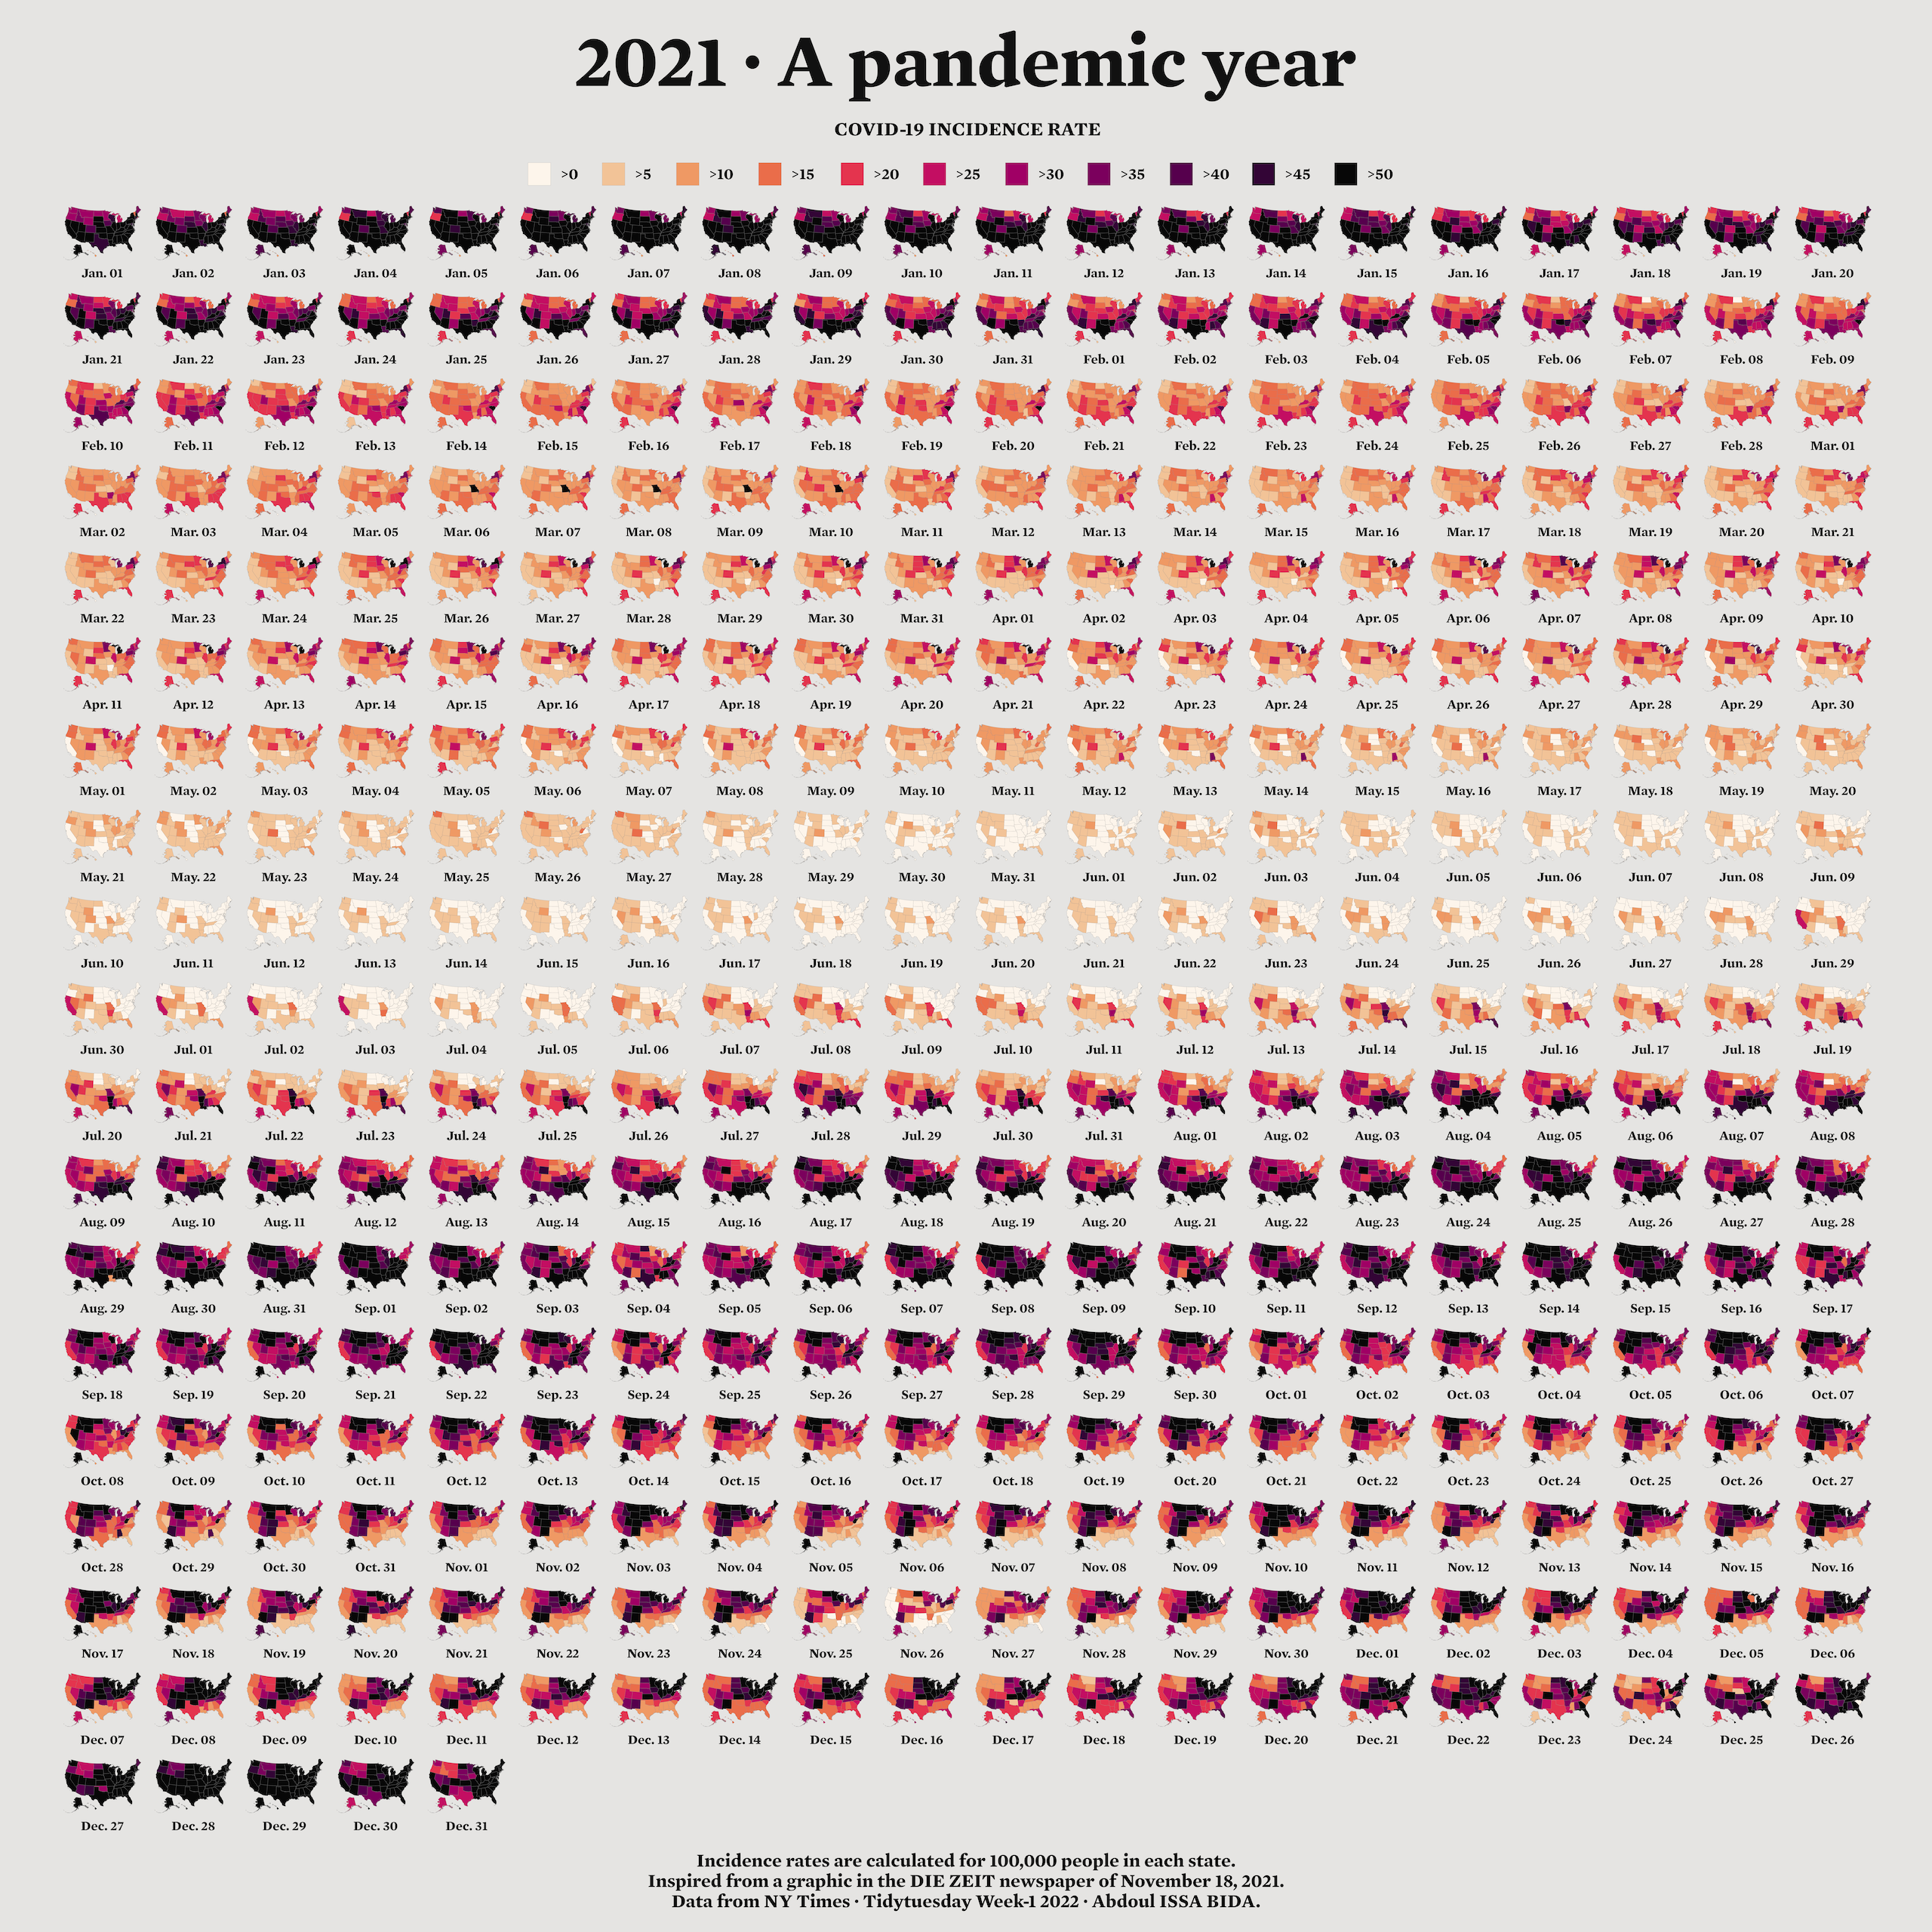
\includegraphics[width=1\linewidth]{assets/covid-map} \caption{Abdoul Madjid's map of COVID in the United States in 2021}\label{fig:madjid-covid-map}
\end{figure}

In this chapter, we'll explore principles of working with simple features geospatial data, then walk through Madjid's code to understand how he created this high-quality map. We'll also discuss where to find geospatial data and how to use it to make your own maps.

\hypertarget{the-briefest-of-primers-on-geospatial-data}{%
\section*{The Briefest of Primers on Geospatial Data}\label{the-briefest-of-primers-on-geospatial-data}}
\addcontentsline{toc}{section}{The Briefest of Primers on Geospatial Data}

You don't need to be a GIS expert to make maps. But you do need to understand a few things about how geospatial data works, starting with its two main types: \emph{vector} and \emph{raster}. Vector data uses points, lines, and polygons to represent the world. Raster data, which often comes from digital photographs, ties each pixel in an image to a specific geographic location. Vector data tends to be easier to work with, and we'll be using it exclusively in this chapter.

In the past, working with geospatial data meant mastering competing standards, each of which required learning a different approach. Today, though, most people use the \emph{simple features} model for working with vector geospatial data (often abbreviated as \emph{sf}), which is way easier to understand. For example, I can import simple features data about the state of Wyoming using this code:

After doing this, I can now take a look at the data:

\begin{Shaded}
\begin{Highlighting}[]
\NormalTok{wyoming}
\CommentTok{\#\textgreater{} Simple feature collection with 1 feature and 1 field}
\CommentTok{\#\textgreater{} Geometry type: POLYGON}
\CommentTok{\#\textgreater{} Dimension:     XY}
\CommentTok{\#\textgreater{} Bounding box:  xmin: {-}111.0546 ymin: 40.99477 xmax: {-}104.0522 ymax: 45.00582}
\CommentTok{\#\textgreater{} Geodetic CRS:  WGS 84}
\CommentTok{\#\textgreater{} \# A tibble: 1 x 2}
\CommentTok{\#\textgreater{}   NAME                                              geometry}
\CommentTok{\#\textgreater{}   \textless{}chr\textgreater{}                                        \textless{}POLYGON [°]\textgreater{}}
\CommentTok{\#\textgreater{} 1 Wyoming (({-}106.32 40.999, {-}106.33 40.999, {-}106.33 40.999,\textasciitilde{}}
\end{Highlighting}
\end{Shaded}

You can see that it has two columns, one for the state name (\texttt{NAME}) and another called \texttt{geometry}. This data looks like the data frames you're used to encountering, aside from two major differences: There is a bunch of metadata above the data frame, and our simple features data contains geographical data in a variable called \texttt{geometry}.

The metadata states that we have one feature and one field. The feature referenced here is the row, and the field is the \texttt{NAME} variable, which contains non-spatial data. Because the \texttt{geometry} column must be present for a data frame to be geospatial data, it is not counted as a field. Let's look at each part of this simple features data.

\hypertarget{geometry-type}{%
\subsection*{Geometry Type}\label{geometry-type}}
\addcontentsline{toc}{subsection}{Geometry Type}

The geometry type represents the shape of the geospatial data we're working with. These types are typically written in all caps. In this case, the relatively simple \texttt{POLYGON} type represents a single polygon. We can use ggplot to display this data by calling \texttt{geom\_sf()}, a special geom designed to work with simple features data:

\begin{Shaded}
\begin{Highlighting}[]
\FunctionTok{library}\NormalTok{(tidyverse)}

\NormalTok{wyoming }\SpecialCharTok{\%\textgreater{}\%}
  \FunctionTok{ggplot}\NormalTok{() }\SpecialCharTok{+}
  \FunctionTok{geom\_sf}\NormalTok{()}
\end{Highlighting}
\end{Shaded}

Figure \ref{fig:wyoming-map-plot} shows the resulting map of Wyoming. It may not look like much, but, hey, I wasn't the one who chose to make Wyoming a nearly perfect rectangle!

\begin{figure}
\includegraphics[width=1\linewidth]{maps_files/figure-latex/wyoming-map-plot-1} \caption{A map of Wyoming}\label{fig:wyoming-map-plot}
\end{figure}

Other geometry types used in simple feature data include \texttt{POINT}, to display elements such as a pin on a map that represents a single location. Try importing data that shows a single electrical vehicle charging station in Wyoming, then placing this data on a map:

\begin{Shaded}
\begin{Highlighting}[]
\NormalTok{wyoming\_one\_ev\_station }\OtherTok{\textless{}{-}} \FunctionTok{read\_sf}\NormalTok{(}\StringTok{"https://data.rwithoutstatistics.com/wyoming{-}one{-}ev{-}station.geojson"}\NormalTok{)}

\FunctionTok{ggplot}\NormalTok{() }\SpecialCharTok{+}
  \FunctionTok{geom\_sf}\NormalTok{(}\AttributeTok{data =}\NormalTok{ wyoming) }\SpecialCharTok{+}
  \FunctionTok{geom\_sf}\NormalTok{(}
    \AttributeTok{data =}\NormalTok{ wyoming\_one\_ev\_station,}
    \AttributeTok{shape =} \DecValTok{21}\NormalTok{,}
    \AttributeTok{fill =} \StringTok{"\#ff7400"}\NormalTok{,}
    \AttributeTok{color =} \StringTok{"white"}\NormalTok{,}
    \AttributeTok{size =} \DecValTok{3}
\NormalTok{  )}
\end{Highlighting}
\end{Shaded}

Figure \ref{fig:ev-stations-map} shows the resulting map.

\begin{figure}
\includegraphics[width=1\linewidth]{maps_files/figure-latex/ev-stations-map-1} \caption{A map of a single electric vehicle charging station in Wyoming}\label{fig:ev-stations-map}
\end{figure}

The \texttt{LINESTRING} geometry type is for a set of points that can be connected with lines, often used to represent roads. We can import and plot the following data to show a \texttt{LINESTRING}:

\begin{Shaded}
\begin{Highlighting}[]
\NormalTok{wyoming\_highway\_30 }\OtherTok{\textless{}{-}} \FunctionTok{read\_sf}\NormalTok{(}\StringTok{"data/wyoming{-}highway{-}30.geojson"}\NormalTok{)}

\NormalTok{wyoming\_highway\_30 }\SpecialCharTok{\%\textgreater{}\%}
  \FunctionTok{ggplot}\NormalTok{() }\SpecialCharTok{+}
  \FunctionTok{geom\_sf}\NormalTok{(}\AttributeTok{data =}\NormalTok{ wyoming) }\SpecialCharTok{+}
  \FunctionTok{geom\_sf}\NormalTok{(}
    \AttributeTok{color =} \StringTok{"\#ff7400"}\NormalTok{,}
    \AttributeTok{linewidth =} \DecValTok{1}
\NormalTok{  )}
\end{Highlighting}
\end{Shaded}

Figure \ref{fig:wy-roads-map} shows us the resulting map, which is a section of US Highway 30 that runs through Wyoming.

\begin{figure}
\includegraphics[width=1\linewidth]{maps_files/figure-latex/wy-roads-map-1} \caption{A map of a section of U.S. Highway 30 running through Wyoming}\label{fig:wy-roads-map}
\end{figure}

Each of these geometry types has a MULTI variation (\texttt{MULTIPOINT}, \texttt{MULTILINESTRING}, and \texttt{MULTIPOLYGON}) that combines multiple instances of the type in one row of data. We can import and plot \texttt{MULTIPOINT} data showing all electric vehicle charging stations in Wyoming using this code:

\begin{Shaded}
\begin{Highlighting}[]
\NormalTok{wyoming\_all\_ev\_stations }\OtherTok{\textless{}{-}} \FunctionTok{read\_sf}\NormalTok{(}\StringTok{"https://data.rwithoutstatistics.com/wyoming{-}all{-}ev{-}stations.geojson"}\NormalTok{)}

\FunctionTok{ggplot}\NormalTok{() }\SpecialCharTok{+}
  \FunctionTok{geom\_sf}\NormalTok{(}\AttributeTok{data =}\NormalTok{ wyoming) }\SpecialCharTok{+}
  \FunctionTok{geom\_sf}\NormalTok{(}
    \AttributeTok{data =}\NormalTok{ wyoming\_all\_ev\_stations,}
    \AttributeTok{fill =} \StringTok{"\#ff7400"}\NormalTok{,}
    \AttributeTok{color =} \StringTok{"white"}\NormalTok{,}
    \AttributeTok{shape =} \DecValTok{21}\NormalTok{,}
    \AttributeTok{size =} \DecValTok{3}
\NormalTok{  )}
\end{Highlighting}
\end{Shaded}

Figure \ref{fig:wyoming-ev-stations-map} shows what the map made from this code looks like.

\begin{figure}
\includegraphics[width=1\linewidth]{maps_files/figure-latex/wyoming-ev-stations-map-1} \caption{A map of all electric vehicle charging stations in Wyoming}\label{fig:wyoming-ev-stations-map}
\end{figure}

Likewise, we can use MULTILINESTRING data to show not just one road, but all major roads in Wyoming:

\begin{Shaded}
\begin{Highlighting}[]
\NormalTok{wyoming\_roads }\OtherTok{\textless{}{-}} \FunctionTok{read\_sf}\NormalTok{(}\StringTok{"https://data.rwithoutstatistics.com/wyoming{-}roads.geojson"}\NormalTok{)}

\NormalTok{wyoming\_roads }\SpecialCharTok{\%\textgreater{}\%}
  \FunctionTok{ggplot}\NormalTok{() }\SpecialCharTok{+}
  \FunctionTok{geom\_sf}\NormalTok{(}\AttributeTok{data =}\NormalTok{ wyoming) }\SpecialCharTok{+}
  \FunctionTok{geom\_sf}\NormalTok{(}
    \AttributeTok{color =} \StringTok{"\#ff7400"}\NormalTok{,}
    \AttributeTok{linewidth =} \DecValTok{1}
\NormalTok{  )}
\end{Highlighting}
\end{Shaded}

Figure \ref{fig:wyoming-roads-map} shows the resulting map.

\begin{figure}
\includegraphics[width=1\linewidth]{maps_files/figure-latex/wyoming-roads-map-1} \caption{A map of all major roads in Wyoming}\label{fig:wyoming-roads-map}
\end{figure}

Lastly, we could use \texttt{MULTIPOLYGON} data to, for example, depict a state made up of multiple polygons. To see what I mean, take a look at a map of Wyoming's counties. We can import data to make this map with the following code:

If we look at the data, we can see how it represents the 23 counties in the state:

\begin{verbatim}
#> Simple feature collection with 23 features and 1 field
#> Geometry type: MULTIPOLYGON
#> Dimension:     XY
#> Bounding box:  xmin: -111.0546 ymin: 40.99477 xmax: -104.0522 ymax: 45.00582
#> Geodetic CRS:  WGS 84
#> # A tibble: 23 x 2
#>    NAME                                             geometry
#>    <chr>                                  <MULTIPOLYGON [°]>
#>  1 Lincoln     (((-110.54 42.287, -110.54 42.286, -110.54 4~
#>  2 Fremont     (((-109.33 42.869, -109.33 42.869, -109.33 4~
#>  3 Uinta       (((-110.58 41.579, -110.58 41.579, -110.58 4~
#>  4 Big Horn    (((-107.5 44.64, -107.5 44.64, -107.5 44.641~
#>  5 Hot Springs (((-108.16 43.471, -108.16 43.46, -108.16 43~
#>  6 Washakie    (((-107.68 44.166, -107.68 44.166, -107.68 4~
#>  7 Converse    (((-105.92 43.495, -105.92 43.495, -105.91 4~
#>  8 Sweetwater  (((-109.57 40.998, -109.57 40.998, -109.57 4~
#>  9 Crook       (((-104.46 44.181, -104.46 44.181, -104.46 4~
#> 10 Carbon      (((-106.32 41.383, -106.32 41.382, -106.32 4~
#> # i 13 more rows
\end{verbatim}

The geometry type of this data is \texttt{MULTIPOLYGON}. In addition, the repeated \texttt{MULTIPOLYGON} text in the geometry column indicates that each row contains a shape of type \texttt{MULTIPOLYGON}.

\begin{Shaded}
\begin{Highlighting}[]
\NormalTok{wyoming\_counties }\SpecialCharTok{\%\textgreater{}\%}
  \FunctionTok{ggplot}\NormalTok{() }\SpecialCharTok{+}
  \FunctionTok{geom\_sf}\NormalTok{(}\AttributeTok{data =}\NormalTok{ wyoming) }\SpecialCharTok{+}
  \FunctionTok{geom\_sf}\NormalTok{()}
\end{Highlighting}
\end{Shaded}

Figure \ref{fig:wyoming-counties-map} is a map made with this data.

\begin{figure}
\includegraphics[width=1\linewidth]{maps_files/figure-latex/wyoming-counties-map-1} \caption{A map of Wyoming counties}\label{fig:wyoming-counties-map}
\end{figure}

You can easily see the multiple polygons that make up the map.

\hypertarget{the-dimensions}{%
\subsection*{The Dimensions}\label{the-dimensions}}
\addcontentsline{toc}{subsection}{The Dimensions}

Next, the geospatial data frame contains the data's \emph{dimensions}, or the type of geospatial data we're working with. In the Wyoming example, it looks like this: \texttt{Dimension:\ XY}, meaning the data is two-dimensional, as in the case of all the geospatial data used in this chapter. There are two other dimensions (\texttt{Z} and \texttt{M}) that you'll see much more rarely. I'll leave them for you to investigate further.

\hypertarget{bounding-box}{%
\subsection*{Bounding Box}\label{bounding-box}}
\addcontentsline{toc}{subsection}{Bounding Box}

The penultimate element in the metadata is the bounding box. A \emph{bounding box} represents the smallest area in which we can fit all of our geospatial data. For our \texttt{wyoming} object, it looks like this:

\texttt{Bounding\ box:\ \ xmin:\ -111.0569\ ymin:\ 40.99475\ xmax:\ -104.0522\ ymax:\ 45.0059}

The \texttt{ymin} value of 40.99475 and \texttt{ymax} value of 45.0059 represent the lowest and highest latitude, respectively, that the state's polygon can fit into. The x values do the same for the longitude. Bounding boxes are calculated automatically, and you don't typically have to worry about altering them.

\hypertarget{the-geodetic-crs}{%
\subsection*{The Geodetic CRS}\label{the-geodetic-crs}}
\addcontentsline{toc}{subsection}{The Geodetic CRS}

The last piece of metadata specifies the \emph{coordinate reference system} used to project our data when we plot it. The problem with representing any geospatial data is that we're displaying information about the three-dimensional Earth on a two-dimensional map. Doing so requires us to choose a coordinate reference system that determines what type of correspondence, or \emph{projection}, to use when making our map.

The data for the Wyoming counties map includes the line \texttt{Geodetic\ CRS:\ WGS\ 84}, indicating the use of a coordinate reference system known as \emph{WGS84}. To see a different projection, check out the same map using what's known as the \emph{Albers equal-area conic convenience projection}:

\begin{Shaded}
\begin{Highlighting}[]
\NormalTok{wyoming\_counties }\SpecialCharTok{\%\textgreater{}\%}
\NormalTok{  sf}\SpecialCharTok{::}\FunctionTok{st\_transform}\NormalTok{(albersusa}\SpecialCharTok{::}\NormalTok{us\_laea\_proj) }\SpecialCharTok{\%\textgreater{}\%}
  \FunctionTok{ggplot}\NormalTok{() }\SpecialCharTok{+}
  \FunctionTok{geom\_sf}\NormalTok{()}
\end{Highlighting}
\end{Shaded}

To use this projection, we add a line that uses the \texttt{st\_transform()} function from the \texttt{sf} package, along with data from the \texttt{albersusa} package, before plotting it using ggplot. While Wyoming looked perfectly horizontal in Figure \ref{fig:wyoming-counties-map}, the version in Figure \ref{fig:wyoming-counties-map-wgs84} appears to be tilted.

\begin{figure}
\includegraphics[width=1\linewidth]{maps_files/figure-latex/wyoming-counties-map-wgs84-1} \caption{A map of Wyoming counties using the Albers equal-area conic convenience projection}\label{fig:wyoming-counties-map-wgs84}
\end{figure}

If you're curious about how to change projections when making maps of your own, fear not. You'll see how to do this when we look at Abdoul Madjid's map in the next section. And if you want to know how to choose appropriate projections for your maps, check out the ``Using Appropriate Projections'' section below.

\hypertarget{the-geometry-column}{%
\subsection*{\texorpdfstring{The \texttt{geometry} Column}{The geometry Column}}\label{the-geometry-column}}
\addcontentsline{toc}{subsection}{The \texttt{geometry} Column}

In addition to the metadata, our simple features data differs from traditional data frames in another respect: its \texttt{geometry} column. As you probably guessed from the name, it holds the data needed to make our maps.

To understand how this works, consider the connect-the-dots drawings you probably completed as a kid. As you added lines to connect one point to the next, the subject of your drawing became clear. The geometry column is similar. It has a set of numbers, each of which corresponds to a point. If you're using \texttt{LINESTRING/MULTILINESTRING} or \texttt{POLYGON/MULTIPOLYGON} simple features data, ggplot uses the numbers in the geometry column to draw each point and then adds lines to connect the points. If you're using \texttt{POINT/MULTIPOINT} data, it draws the points but doesn't connect them.

Once again, you never have to worry about these details or look in any depth at the \texttt{geometry} column.

\hypertarget{recreating-the-covid-map}{%
\section*{Recreating the COVID Map}\label{recreating-the-covid-map}}
\addcontentsline{toc}{section}{Recreating the COVID Map}

Now that you understand the basics of geospatial data, let's walk through the code Madjid used to make his COVID-19 map, which makes use of the geometry types, dimensions, bounding boxes, projections, and the geometry column we just explored. (I've made some small modifications to the code to make the final map fit on the page.) Let's begin by loading few packages:

\begin{Shaded}
\begin{Highlighting}[]
\FunctionTok{library}\NormalTok{(tidyverse)}
\FunctionTok{library}\NormalTok{(albersusa)}
\FunctionTok{library}\NormalTok{(sf)}
\FunctionTok{library}\NormalTok{(zoo)}
\FunctionTok{library}\NormalTok{(colorspace)}
\end{Highlighting}
\end{Shaded}

The \texttt{albersusa} package will give us access to geospatial data, and you can install it as follows:

\begin{Shaded}
\begin{Highlighting}[]
\NormalTok{remotes}\SpecialCharTok{::}\FunctionTok{install\_github}\NormalTok{(}\StringTok{"hrbrmstr/albersusa"}\NormalTok{)}
\end{Highlighting}
\end{Shaded}

You can install all of the other packages using the standard \texttt{install.packages()} code. We'll use \texttt{tidyverse} to import data, manipulate it, and plot it with ggplot. The \texttt{sf} package will enable us to change the coordinate reference system and use an appropriate projection for the data. The \texttt{zoo} package has functions for calculating rolling averages, and the \texttt{colorspace} package gives us a color scale that highlights the data well.

\hypertarget{importing-the-data}{%
\subsection*{Importing the Data}\label{importing-the-data}}
\addcontentsline{toc}{subsection}{Importing the Data}

Next, let's import the data we need. We require three pieces of data: COVID rates by state over time, state populations, and geospatial information. Madjid imported each of these pieces of data separately and then merged them, and we'll do the same.

First, we import COVID data. This data comes directly from \emph{The New York Times}, which publishes daily case rates by state as a CSV file on its GitHub account. I've dropped the \texttt{fips} variable; Federal Information Processing Standards (FIPS) are numeric codes used to represent states, but we can reference states by their names instead:

\begin{Shaded}
\begin{Highlighting}[]
\NormalTok{covid\_data }\OtherTok{\textless{}{-}} \FunctionTok{read\_csv}\NormalTok{(}\StringTok{"https://data.rwithoutstatistics.com/covid{-}us{-}states.csv"}\NormalTok{) }\SpecialCharTok{\%\textgreater{}\%}
  \FunctionTok{select}\NormalTok{(}\SpecialCharTok{{-}}\NormalTok{fips)}
\end{Highlighting}
\end{Shaded}

If you take a look at this data, you can see the arrival of the first COVID cases in the United States in January 2020.

\begin{verbatim}
#> # A tibble: 61,102 x 4
#>    date       state      cases deaths
#>    <date>     <chr>      <dbl>  <dbl>
#>  1 2020-01-21 Washington     1      0
#>  2 2020-01-22 Washington     1      0
#>  3 2020-01-23 Washington     1      0
#>  4 2020-01-24 Illinois       1      0
#>  5 2020-01-24 Washington     1      0
#>  6 2020-01-25 California     1      0
#>  7 2020-01-25 Illinois       1      0
#>  8 2020-01-25 Washington     1      0
#>  9 2020-01-26 Arizona        1      0
#> 10 2020-01-26 California     2      0
#> # i 61,092 more rows
\end{verbatim}

Madjid's map shows per capita rates (rates per 100,000 people) rather than absolute rates (the rates without consideration for a state's population). So, to recreate his maps, we need to obtain data on each state's population. Madjid downloaded this data as a CSV:

\begin{Shaded}
\begin{Highlighting}[]
\NormalTok{usa\_states }\OtherTok{\textless{}{-}} \FunctionTok{read\_csv}\NormalTok{(}\StringTok{"https://data.rwithoutstatistics.com/population{-}by{-}state.csv"}\NormalTok{) }\SpecialCharTok{\%\textgreater{}\%}
  \FunctionTok{select}\NormalTok{(State, Pop)}
\end{Highlighting}
\end{Shaded}

We import this data, keep the \texttt{State} and \texttt{Pop} (population) variables, and save it as an object called \texttt{usa\_states}. Let's see what \texttt{usa\_states} looks like:

\begin{verbatim}
#> # A tibble: 52 x 2
#>    State               Pop
#>    <chr>             <dbl>
#>  1 California     39613493
#>  2 Texas          29730311
#>  3 Florida        21944577
#>  4 New York       19299981
#>  5 Pennsylvania   12804123
#>  6 Illinois       12569321
#>  7 Ohio           11714618
#>  8 Georgia        10830007
#>  9 North Carolina 10701022
#> 10 Michigan        9992427
#> # i 42 more rows
\end{verbatim}

Finally, we'll import the geospatial data and save it as an object called \texttt{usa\_states\_geom}:

\begin{Shaded}
\begin{Highlighting}[]
\NormalTok{usa\_states\_geom }\OtherTok{\textless{}{-}} \FunctionTok{usa\_sf}\NormalTok{() }\SpecialCharTok{\%\textgreater{}\%}
  \FunctionTok{select}\NormalTok{(name) }\SpecialCharTok{\%\textgreater{}\%}
  \FunctionTok{st\_transform}\NormalTok{(us\_laea\_proj)}
\end{Highlighting}
\end{Shaded}

The \texttt{usa\_sf()} function from the \texttt{albersusa} package gives us simple features data for all US states. Conveniently, it places Alaska and Hawaii in locations, and at a scale, that make them easy to see. This data includes multiple variables, but we need only the state names, so we keep the \texttt{name} variable only.

We then use the \texttt{st\_transform()} function from the \texttt{sf} package to change the coordinate reference system. The one used here comes from the \texttt{us\_laea\_proj} object in the albersusa package. Remember the \emph{Albers equal-area conic convenience} projection we used to change the appearance of our Wyoming counties map? This is the same projection.

\hypertarget{calculating-daily-covid-cases}{%
\subsection*{Calculating Daily COVID Cases}\label{calculating-daily-covid-cases}}
\addcontentsline{toc}{subsection}{Calculating Daily COVID Cases}

Next, we need to calculate the number of daily COVID cases. We have to do this because the \texttt{covid\_data} data frame gives us cumulative cases by state, but not the number of cases per day:

\begin{Shaded}
\begin{Highlighting}[]
\NormalTok{covid\_cases }\OtherTok{\textless{}{-}}\NormalTok{ covid\_data }\SpecialCharTok{\%\textgreater{}\%}
  \FunctionTok{group\_by}\NormalTok{(state) }\SpecialCharTok{\%\textgreater{}\%}
  \FunctionTok{mutate}\NormalTok{(}
    \AttributeTok{pd\_cases =} \FunctionTok{lag}\NormalTok{(cases)}
\NormalTok{  ) }\SpecialCharTok{\%\textgreater{}\%}
  \FunctionTok{replace\_na}\NormalTok{(}\FunctionTok{list}\NormalTok{(}\AttributeTok{pd\_cases =} \DecValTok{0}\NormalTok{)) }\SpecialCharTok{\%\textgreater{}\%}
  \FunctionTok{mutate}\NormalTok{(}
    \AttributeTok{daily\_cases =} \FunctionTok{case\_when}\NormalTok{(}
\NormalTok{      cases }\SpecialCharTok{\textgreater{}}\NormalTok{ pd\_cases }\SpecialCharTok{\textasciitilde{}}\NormalTok{ cases }\SpecialCharTok{{-}}\NormalTok{ pd\_cases,}
      \ConstantTok{TRUE} \SpecialCharTok{\textasciitilde{}} \DecValTok{0}
\NormalTok{    )}
\NormalTok{  ) }\SpecialCharTok{\%\textgreater{}\%}
  \FunctionTok{ungroup}\NormalTok{() }\SpecialCharTok{\%\textgreater{}\%}
  \FunctionTok{arrange}\NormalTok{(state, date)}
\end{Highlighting}
\end{Shaded}

We use the \texttt{group\_by()} function to calculate totals for each state, then create a new variable called \texttt{pd\_cases}, which represents the number of cases in the previous day (we can use the \texttt{lag()} function to assign data to this variable). Some days do not have cases counts for the previous day, so in these cases, we set the value to 0 using the \texttt{replace\_na()} function.

Finally, we create a new variable called \texttt{daily\_cases}. To set the value of this variable, we use the \texttt{case\_when()} function to create a condition: If the cases variable (which holds the cases on that day) is greater than the \texttt{pd\_cases} variable (which holds cases from one day prior), then \texttt{daily\_cases} is equal to cases minus pd\_cases. Otherwise, we set \texttt{daily\_cases} to be equal to 0.

Because we grouped the data by state at the beginning, we must now remove this grouping using the \texttt{ungroup()} function before arranging our data by state and date. Now take a look at the \texttt{covid\_cases} data frame we created:

\begin{verbatim}
#> # A tibble: 61,102 x 6
#>    date       state   cases deaths pd_cases daily_cases
#>    <date>     <chr>   <dbl>  <dbl>    <dbl>       <dbl>
#>  1 2020-03-13 Alabama     6      0        0           6
#>  2 2020-03-14 Alabama    12      0        6           6
#>  3 2020-03-15 Alabama    23      0       12          11
#>  4 2020-03-16 Alabama    29      0       23           6
#>  5 2020-03-17 Alabama    39      0       29          10
#>  6 2020-03-18 Alabama    51      0       39          12
#>  7 2020-03-19 Alabama    78      0       51          27
#>  8 2020-03-20 Alabama   106      0       78          28
#>  9 2020-03-21 Alabama   131      0      106          25
#> 10 2020-03-22 Alabama   157      0      131          26
#> # i 61,092 more rows
\end{verbatim}

In the next step, we'll make use of the \texttt{daily\_cases} variable.

\hypertarget{calculating-incidence-rates}{%
\subsection*{Calculating Incidence Rates}\label{calculating-incidence-rates}}
\addcontentsline{toc}{subsection}{Calculating Incidence Rates}

We're not quite done calculating values. The data that Madjid used to make his map didn't include daily case counts. Instead, it contained a five-day rolling average of cases per 100,000 people. A \emph{rolling average} is the average case rate in a certain time period. Quirks of reporting (for example, not reporting on weekends but instead rolling Saturday and Sunday cases into Monday) can make the value for any single day less reliable. Using a rolling average smooths things out. Here is the code to generate this data:

\begin{Shaded}
\begin{Highlighting}[]
\NormalTok{covid\_cases }\SpecialCharTok{\%\textgreater{}\%}
  \FunctionTok{mutate}\NormalTok{(}\AttributeTok{roll\_cases =} \FunctionTok{rollmean}\NormalTok{(}
\NormalTok{    daily\_cases,}
    \AttributeTok{k =} \DecValTok{5}\NormalTok{,}
    \AttributeTok{fill =} \ConstantTok{NA}
\NormalTok{  ))}
\end{Highlighting}
\end{Shaded}

We create a new data frame called \texttt{covid\_cases\_rm} (where \emph{rm} stands for rolling mean). The first step in its creation is to use the \texttt{rollmean()} function from the \texttt{zoo} package to create a roll\_cases variable, which holds the average number of cases in the five-day period surrounding a single date. The \texttt{k} argument is the number of days for which we want to calculate the rolling average (five, in our case), and the \texttt{fill} argument determines what happens in cases like the first day, where we can't calculate a five-day rolling mean because there are no days prior to this day (Madjid set these values to be NA).

After calculating \texttt{roll\_cases}, we need to calculate per capita case rates. To do this, we needed population data, so we join the population data from the \texttt{usa\_states} data frame with the \texttt{covid\_cases} data:

\begin{Shaded}
\begin{Highlighting}[]
\NormalTok{covid\_cases\_rm }\OtherTok{\textless{}{-}}\NormalTok{ covid\_cases }\SpecialCharTok{\%\textgreater{}\%}
  \FunctionTok{mutate}\NormalTok{(}\AttributeTok{roll\_cases =} \FunctionTok{rollmean}\NormalTok{(}
\NormalTok{    daily\_cases,}
    \AttributeTok{k =} \DecValTok{5}\NormalTok{,}
    \AttributeTok{fill =} \ConstantTok{NA}
\NormalTok{  )) }\SpecialCharTok{\%\textgreater{}\%}
  \FunctionTok{left\_join}\NormalTok{(}
\NormalTok{    usa\_states,}
    \AttributeTok{by =} \FunctionTok{c}\NormalTok{(}\StringTok{"state"} \OtherTok{=} \StringTok{"State"}\NormalTok{)}
\NormalTok{  ) }\SpecialCharTok{\%\textgreater{}\%}
  \FunctionTok{drop\_na}\NormalTok{(Pop)}
\end{Highlighting}
\end{Shaded}

We then drop rows with missing population data (the \texttt{Pop} variable). In practice, this means getting rid of several US territories (American Samoa, Guam, Northern Marianas Islands, and Virgin Islands).

Next, we created a per capita case rate variable called \texttt{incidence\_rate} by multiplying the \texttt{roll\_cases} variable by 100,000 and then dividing it by the population of each state:

\begin{Shaded}
\begin{Highlighting}[]
\NormalTok{covid\_cases\_rm }\OtherTok{\textless{}{-}}\NormalTok{ covid\_cases\_rm }\SpecialCharTok{\%\textgreater{}\%}
  \FunctionTok{mutate}\NormalTok{(}\AttributeTok{incidence\_rate =} \DecValTok{10}\SpecialCharTok{\^{}}\DecValTok{5} \SpecialCharTok{*}\NormalTok{ roll\_cases }\SpecialCharTok{/}\NormalTok{ Pop) }\SpecialCharTok{\%\textgreater{}\%}
  \FunctionTok{mutate}\NormalTok{(}
    \AttributeTok{incidence\_rate =} \FunctionTok{cut}\NormalTok{(}
\NormalTok{      incidence\_rate,}
      \AttributeTok{breaks =} \FunctionTok{c}\NormalTok{(}\FunctionTok{seq}\NormalTok{(}\DecValTok{0}\NormalTok{, }\DecValTok{50}\NormalTok{, }\DecValTok{5}\NormalTok{), }\ConstantTok{Inf}\NormalTok{),}
      \AttributeTok{include.lowest =} \ConstantTok{TRUE}
\NormalTok{    ) }\SpecialCharTok{\%\textgreater{}\%}
      \FunctionTok{factor}\NormalTok{(}\AttributeTok{labels =} \FunctionTok{paste0}\NormalTok{(}\StringTok{"\textgreater{}"}\NormalTok{, }\FunctionTok{seq}\NormalTok{(}\DecValTok{0}\NormalTok{, }\DecValTok{50}\NormalTok{, }\DecValTok{5}\NormalTok{)))}
\NormalTok{  )}
\end{Highlighting}
\end{Shaded}

Rather than keeping raw values (for example, on June 29, 2021, Florida had a rate of 57.77737 cases per 100,000 people), we use the \texttt{cut()} function to convert the values into categories: values of \texttt{\textgreater{}0} (greater than zero), values of \texttt{\textgreater{}5} (greater than five), and values of \texttt{\textgreater{}50} (greater than 50).

The last step is to filter the data so it includes only 2021 data (the only year depicted in Madjid's map) and select only the variables (\texttt{state}, \texttt{date}, and \texttt{incidence\_rate}) we'll need to create our map. Here is the final \texttt{covid\_cases\_rm} data frame.

\begin{verbatim}
#> # A tibble: 18,980 x 3
#>    state   date       incidence_rate
#>    <chr>   <date>     <fct>         
#>  1 Alabama 2021-01-01 >50           
#>  2 Alabama 2021-01-02 >50           
#>  3 Alabama 2021-01-03 >50           
#>  4 Alabama 2021-01-04 >50           
#>  5 Alabama 2021-01-05 >50           
#>  6 Alabama 2021-01-06 >50           
#>  7 Alabama 2021-01-07 >50           
#>  8 Alabama 2021-01-08 >50           
#>  9 Alabama 2021-01-09 >50           
#> 10 Alabama 2021-01-10 >50           
#> # i 18,970 more rows
\end{verbatim}

We now have a data frame that we can combine with our geospatial data.

\hypertarget{adding-geospatial-data}{%
\subsection*{Adding Geospatial Data}\label{adding-geospatial-data}}
\addcontentsline{toc}{subsection}{Adding Geospatial Data}

We've now used two of our three data sources (COVID case data and state population data) to create the \texttt{covid\_cases\_rm} data frame we'll need to make the map. Let's now use the third data source: the geospatial data we saved as \texttt{usa\_states\_geom.} Simple features data allows us to merge regular data frames and geospatial data, another mark in its favor:

\begin{Shaded}
\begin{Highlighting}[]
\NormalTok{usa\_states\_geom }\SpecialCharTok{\%\textgreater{}\%}
  \FunctionTok{left\_join}\NormalTok{(covid\_cases\_rm, }\AttributeTok{by =} \FunctionTok{c}\NormalTok{(}\StringTok{"name"} \OtherTok{=} \StringTok{"state"}\NormalTok{))}
\end{Highlighting}
\end{Shaded}

We merge our \texttt{covid\_cases\_rm} data frame into the geospatial data, matching the name variable from \texttt{usa\_states\_geom} to the state variable in \texttt{covid\_cases\_rm}. Next, we create a new variable called \texttt{fancy\_date.} As the name implies, it's a nicely formatted version of the date (for example, \emph{Jan 01} instead of \emph{2021-01-01}):

\begin{Shaded}
\begin{Highlighting}[]
\NormalTok{usa\_states\_geom\_covid }\OtherTok{\textless{}{-}}\NormalTok{ usa\_states\_geom }\SpecialCharTok{\%\textgreater{}\%}
  \FunctionTok{left\_join}\NormalTok{(covid\_cases\_rm, }\AttributeTok{by =} \FunctionTok{c}\NormalTok{(}\StringTok{"name"} \OtherTok{=} \StringTok{"state"}\NormalTok{)) }\SpecialCharTok{\%\textgreater{}\%}
  \FunctionTok{mutate}\NormalTok{(}\AttributeTok{fancy\_date =} \FunctionTok{fct\_inorder}\NormalTok{(}\FunctionTok{format}\NormalTok{(date, }\StringTok{"\%b. \%d"}\NormalTok{))) }\SpecialCharTok{\%\textgreater{}\%}
  \FunctionTok{relocate}\NormalTok{(fancy\_date, }\AttributeTok{.before =}\NormalTok{ incidence\_rate)}
\end{Highlighting}
\end{Shaded}

The \texttt{format()} function does the formatting while the \texttt{fct\_inorder()} function makes the \texttt{fancy\_date} variable sort data by date (rather than, say, alphabetically, which would put August before January). Last, we use the \texttt{relocate()} function to put the \texttt{fancy\_date} column next to the date column. We save this data frame as \texttt{usa\_states\_geom\_covid}. Take a look at it:

\begin{verbatim}
#> Simple feature collection with 18615 features and 4 fields
#> Geometry type: MULTIPOLYGON
#> Dimension:     XY
#> Bounding box:  xmin: -2100000 ymin: -2500000 xmax: 2516374 ymax: 732103.3
#> Projected CRS: +proj=laea +lat_0=45 +lon_0=-100 +x_0=0 +y_0=0 +a=6370997 +b=6370997 +units=m +no_defs
#> First 10 features:
#>       name       date fancy_date incidence_rate
#> 1  Arizona 2021-01-01    Jan. 01            >50
#> 2  Arizona 2021-01-02    Jan. 02            >50
#> 3  Arizona 2021-01-03    Jan. 03            >50
#> 4  Arizona 2021-01-04    Jan. 04            >50
#> 5  Arizona 2021-01-05    Jan. 05            >50
#> 6  Arizona 2021-01-06    Jan. 06            >50
#> 7  Arizona 2021-01-07    Jan. 07            >50
#> 8  Arizona 2021-01-08    Jan. 08            >50
#> 9  Arizona 2021-01-09    Jan. 09            >50
#> 10 Arizona 2021-01-10    Jan. 10            >50
#>                          geometry
#> 1  MULTIPOLYGON (((-1111066 -8...
#> 2  MULTIPOLYGON (((-1111066 -8...
#> 3  MULTIPOLYGON (((-1111066 -8...
#> 4  MULTIPOLYGON (((-1111066 -8...
#> 5  MULTIPOLYGON (((-1111066 -8...
#> 6  MULTIPOLYGON (((-1111066 -8...
#> 7  MULTIPOLYGON (((-1111066 -8...
#> 8  MULTIPOLYGON (((-1111066 -8...
#> 9  MULTIPOLYGON (((-1111066 -8...
#> 10 MULTIPOLYGON (((-1111066 -8...
\end{verbatim}

We can see the metadata and \texttt{geometry} columns we discussed.

\hypertarget{making-the-map}{%
\subsection*{Making the Map}\label{making-the-map}}
\addcontentsline{toc}{subsection}{Making the Map}

It took a lot of work to end up with the surprisingly simple data frame \texttt{usa\_states\_geom\_covid}. And while the data may be simple, the code Madjid used to make his map is quite complex. In this section, we walk through it in pieces.

The final map is actually multiple maps, one for each day in 2021. Combining 365 days makes for a large final product, so instead of showing the code for every single day, we'll filter the \texttt{usa\_states\_geom\_covid} to show just the first six days in January:

\begin{Shaded}
\begin{Highlighting}[]
\NormalTok{usa\_states\_geom\_covid\_six\_days }\OtherTok{\textless{}{-}}\NormalTok{ usa\_states\_geom\_covid }\SpecialCharTok{\%\textgreater{}\%}
  \FunctionTok{filter}\NormalTok{(date }\SpecialCharTok{\textless{}=} \FunctionTok{as.Date}\NormalTok{(}\StringTok{"2021{-}01{-}06"}\NormalTok{))}
\end{Highlighting}
\end{Shaded}

We save the result as a data frame called \texttt{usa\_states\_geom\_covid\_six\_days}. Here's what this data looks like:

\begin{verbatim}
#> Simple feature collection with 306 features and 4 fields
#> Geometry type: MULTIPOLYGON
#> Dimension:     XY
#> Bounding box:  xmin: -2100000 ymin: -2500000 xmax: 2516374 ymax: 732103.3
#> Projected CRS: +proj=laea +lat_0=45 +lon_0=-100 +x_0=0 +y_0=0 +a=6370997 +b=6370997 +units=m +no_defs
#> First 10 features:
#>        name       date fancy_date incidence_rate
#> 1   Arizona 2021-01-01    Jan. 01            >50
#> 2   Arizona 2021-01-02    Jan. 02            >50
#> 3   Arizona 2021-01-03    Jan. 03            >50
#> 4   Arizona 2021-01-04    Jan. 04            >50
#> 5   Arizona 2021-01-05    Jan. 05            >50
#> 6   Arizona 2021-01-06    Jan. 06            >50
#> 7  Arkansas 2021-01-01    Jan. 01            >50
#> 8  Arkansas 2021-01-02    Jan. 02            >50
#> 9  Arkansas 2021-01-03    Jan. 03            >50
#> 10 Arkansas 2021-01-04    Jan. 04            >50
#>                          geometry
#> 1  MULTIPOLYGON (((-1111066 -8...
#> 2  MULTIPOLYGON (((-1111066 -8...
#> 3  MULTIPOLYGON (((-1111066 -8...
#> 4  MULTIPOLYGON (((-1111066 -8...
#> 5  MULTIPOLYGON (((-1111066 -8...
#> 6  MULTIPOLYGON (((-1111066 -8...
#> 7  MULTIPOLYGON (((557903.1 -1...
#> 8  MULTIPOLYGON (((557903.1 -1...
#> 9  MULTIPOLYGON (((557903.1 -1...
#> 10 MULTIPOLYGON (((557903.1 -1...
\end{verbatim}

Madjid's map is giant, as it includes all 365 days. We'll change the size of a few elements so they fit in this book.

\hypertarget{generating-the-basic-map}{%
\subsubsection*{Generating the Basic Map}\label{generating-the-basic-map}}
\addcontentsline{toc}{subsubsection}{Generating the Basic Map}

Now that we have six days of data, let's make some maps. Abdoul Madjid's map-making code has two main parts: generating the basic map, then tweaking its appearance. We'll revisit the three lines of code used to make our Wyoming maps, with some adornments to improve the quality of the visualization:

\begin{Shaded}
\begin{Highlighting}[]
\NormalTok{usa\_states\_geom\_covid\_six\_days }\SpecialCharTok{\%\textgreater{}\%}
  \FunctionTok{ggplot}\NormalTok{() }\SpecialCharTok{+}
  \FunctionTok{geom\_sf}\NormalTok{(}
    \FunctionTok{aes}\NormalTok{(}\AttributeTok{fill =}\NormalTok{ incidence\_rate),}
    \AttributeTok{size =}\NormalTok{ .}\DecValTok{05}\NormalTok{,}
    \AttributeTok{color =} \StringTok{"grey55"}
\NormalTok{  ) }\SpecialCharTok{+}
  \FunctionTok{facet\_wrap}\NormalTok{(}
    \FunctionTok{vars}\NormalTok{(fancy\_date),}
    \AttributeTok{strip.position =} \StringTok{"bottom"}
\NormalTok{  )}
\end{Highlighting}
\end{Shaded}

We use \texttt{geom\_sf()} to plot the geospatial data, modifying a couple arguments. We use \texttt{size\ =\ .05} to make the state borders less prominent and \texttt{color\ =\ "grey55"} to set the borders to a medium gray color. Then, to make one map for each day, we use the \texttt{facet\_wrap()} function. The \texttt{vars(fancy\_date)} code specifies that the \texttt{fancy\_date} variable should be used to do the faceting (in other words, make one map for each day) and \texttt{strip.position\ =\ "bottom"} moves the labels \emph{Jan.~01}, \emph{Jan.~02}, and so on to the bottom of the maps. You can see the resulting map in Figure \ref{fig:basic-map}.

\begin{figure}
\includegraphics[width=1\linewidth]{maps_files/figure-latex/basic-map-1} \caption{A map showing the incidence rate of COVID for the first six days of 2021}\label{fig:basic-map}
\end{figure}

Having generated the basic map, let's now make it look good.

\hypertarget{applying-data-visualization-principles-to-the-map}{%
\subsubsection*{Applying Data Visualization Principles to the Map}\label{applying-data-visualization-principles-to-the-map}}
\addcontentsline{toc}{subsubsection}{Applying Data Visualization Principles to the Map}

From now on, all of the code that Abdoul Madjid uses is to improve the appearance of the maps. Many of the tweaks shown here will feel familiar if you've read Chapter \ref{data-viz-chapter}, highlighting a benefit of making maps with ggplot: You can apply the same data-visualization principles you learned about when making charts.

\begin{Shaded}
\begin{Highlighting}[]
\NormalTok{usa\_states\_geom\_covid\_six\_days }\SpecialCharTok{\%\textgreater{}\%}
  \FunctionTok{ggplot}\NormalTok{() }\SpecialCharTok{+}
  \FunctionTok{geom\_sf}\NormalTok{(}
    \FunctionTok{aes}\NormalTok{(}\AttributeTok{fill =}\NormalTok{ incidence\_rate),}
    \AttributeTok{size =}\NormalTok{ .}\DecValTok{05}\NormalTok{,}
    \AttributeTok{color =} \StringTok{"transparent"}
\NormalTok{  ) }\SpecialCharTok{+}
  \FunctionTok{facet\_wrap}\NormalTok{(}
    \FunctionTok{vars}\NormalTok{(fancy\_date),}
    \AttributeTok{strip.position =} \StringTok{"bottom"}
\NormalTok{  ) }\SpecialCharTok{+}
  \FunctionTok{scale\_fill\_discrete\_sequential}\NormalTok{(}
    \AttributeTok{palette =} \StringTok{"Rocket"}\NormalTok{,}
    \AttributeTok{name =} \StringTok{"COVID{-}19 INCIDENCE RATE"}\NormalTok{,}
    \AttributeTok{guide =} \FunctionTok{guide\_legend}\NormalTok{(}
      \AttributeTok{title.position =} \StringTok{"top"}\NormalTok{,}
      \AttributeTok{title.hjust =}\NormalTok{ .}\DecValTok{5}\NormalTok{,}
      \AttributeTok{title.theme =} \FunctionTok{element\_text}\NormalTok{(}
        \AttributeTok{family =} \StringTok{"Times New Roman"}\NormalTok{,}
        \AttributeTok{size =} \FunctionTok{rel}\NormalTok{(}\DecValTok{9}\NormalTok{),}
        \AttributeTok{margin =} \FunctionTok{margin}\NormalTok{(}
          \AttributeTok{b =}\NormalTok{ .}\DecValTok{1}\NormalTok{,}
          \AttributeTok{unit =} \StringTok{"cm"}
\NormalTok{        )}
\NormalTok{      ),}
      \AttributeTok{nrow =} \DecValTok{1}\NormalTok{,}
      \AttributeTok{keyheight =} \FunctionTok{unit}\NormalTok{(.}\DecValTok{3}\NormalTok{, }\StringTok{"cm"}\NormalTok{),}
      \AttributeTok{keywidth =} \FunctionTok{unit}\NormalTok{(.}\DecValTok{3}\NormalTok{, }\StringTok{"cm"}\NormalTok{),}
      \AttributeTok{label.theme =} \FunctionTok{element\_text}\NormalTok{(}
        \AttributeTok{family =} \StringTok{"Times New Roman"}\NormalTok{,}
        \AttributeTok{size =} \FunctionTok{rel}\NormalTok{(}\DecValTok{6}\NormalTok{),}
        \AttributeTok{margin =} \FunctionTok{margin}\NormalTok{(}
          \AttributeTok{r =} \DecValTok{5}\NormalTok{,}
          \AttributeTok{unit =} \StringTok{"pt"}
\NormalTok{        )}
\NormalTok{      )}
\NormalTok{    )}
\NormalTok{  ) }\SpecialCharTok{+}
  \FunctionTok{labs}\NormalTok{(}
    \AttributeTok{title =} \StringTok{"2021 · A pandemic year"}\NormalTok{,}
    \AttributeTok{caption =} \StringTok{"Incidence rates are calculated for 100,000 people in each state.}
\StringTok{                  Inspired from a graphic in the DIE ZEIT newspaper of November 18, 2021.}
\StringTok{                  Data from NY Times · Tidytuesday Week{-}1 2022 · Abdoul ISSA BIDA."}
\NormalTok{  ) }\SpecialCharTok{+}
  \FunctionTok{theme\_minimal}\NormalTok{() }\SpecialCharTok{+}
  \FunctionTok{theme}\NormalTok{(}
    \AttributeTok{text =} \FunctionTok{element\_text}\NormalTok{(}
      \AttributeTok{family =} \StringTok{"Times New Roman"}\NormalTok{,}
      \AttributeTok{color =} \StringTok{"\#111111"}
\NormalTok{    ),}
    \AttributeTok{plot.title =} \FunctionTok{element\_text}\NormalTok{(}
      \AttributeTok{size =} \FunctionTok{rel}\NormalTok{(}\FloatTok{2.5}\NormalTok{),}
      \AttributeTok{face =} \StringTok{"bold"}\NormalTok{,}
      \AttributeTok{hjust =} \FloatTok{0.5}\NormalTok{,}
      \AttributeTok{margin =} \FunctionTok{margin}\NormalTok{(}
        \AttributeTok{t =}\NormalTok{ .}\DecValTok{25}\NormalTok{,}
        \AttributeTok{b =}\NormalTok{ .}\DecValTok{25}\NormalTok{,}
        \AttributeTok{unit =} \StringTok{"cm"}
\NormalTok{      )}
\NormalTok{    ),}
    \AttributeTok{plot.caption =} \FunctionTok{element\_text}\NormalTok{(}
      \AttributeTok{hjust =}\NormalTok{ .}\DecValTok{5}\NormalTok{,}
      \AttributeTok{face =} \StringTok{"bold"}\NormalTok{,}
      \AttributeTok{margin =} \FunctionTok{margin}\NormalTok{(}
        \AttributeTok{t =}\NormalTok{ .}\DecValTok{25}\NormalTok{,}
        \AttributeTok{b =}\NormalTok{ .}\DecValTok{25}\NormalTok{,}
        \AttributeTok{unit =} \StringTok{"cm"}
\NormalTok{      )}
\NormalTok{    ),}
    \AttributeTok{strip.text =} \FunctionTok{element\_text}\NormalTok{(}
      \AttributeTok{size =} \FunctionTok{rel}\NormalTok{(}\FloatTok{0.75}\NormalTok{),}
      \AttributeTok{face =} \StringTok{"bold"}
\NormalTok{    ),}
    \AttributeTok{legend.position =} \StringTok{"top"}\NormalTok{,}
    \AttributeTok{legend.box.spacing =} \FunctionTok{unit}\NormalTok{(.}\DecValTok{25}\NormalTok{, }\StringTok{"cm"}\NormalTok{),}
    \AttributeTok{panel.grid =} \FunctionTok{element\_blank}\NormalTok{(),}
    \AttributeTok{axis.text =} \FunctionTok{element\_blank}\NormalTok{(),}
    \AttributeTok{plot.margin =} \FunctionTok{margin}\NormalTok{(}
      \AttributeTok{t =}\NormalTok{ .}\DecValTok{25}\NormalTok{,}
      \AttributeTok{r =}\NormalTok{ .}\DecValTok{25}\NormalTok{,}
      \AttributeTok{b =}\NormalTok{ .}\DecValTok{25}\NormalTok{,}
      \AttributeTok{l =}\NormalTok{ .}\DecValTok{25}\NormalTok{,}
      \AttributeTok{unit =} \StringTok{"cm"}
\NormalTok{    ),}
    \AttributeTok{plot.background =} \FunctionTok{element\_rect}\NormalTok{(}
      \AttributeTok{fill =} \StringTok{"\#e5e4e2"}\NormalTok{,}
      \AttributeTok{color =} \ConstantTok{NA}
\NormalTok{    )}
\NormalTok{  )}
\end{Highlighting}
\end{Shaded}

The \texttt{scale\_fill\_discrete\_sequential()} function from the \texttt{colorspace} package sets the color scale. Madjid uses the ``rocket'' palette (the same palette that that Cédric Scherer and Georgios Karamanis used in Chapter \ref{data-viz-chapter}) and changes the legend title to ``COVID-19 INCIDENCE RATE.'' Within the \texttt{guide\_legend()} function, Madjid puts adjusts the position and alignment as well as text properties of the title. He also puts the colored squares in one row, adjusts their height and width, and tweaks the text properties of the labels (the \texttt{\textgreater{}0}, \texttt{\textgreater{}5}, and so on).

Next, he adds a title and caption using the \texttt{labs()} function. After this, he uses \texttt{theme\_minimal()} before making tweaks using the \texttt{theme()} function. These tweaks include setting the font and text color, making the title and caption bold, and adjusting their size, alignment, and the margins around them. He also adjusts the size of the strip text (the \emph{Jan 01}, \emph{Jan 02}, and so on) and makes it bold, puts the legend at the top of the maps, and adds a bit of spacing around it. He removes grid lines and the longitude and latitude lines, then adds a bit of padding around the entire visualization and makes the background a light gray.

There we have it: Figure \ref{fig:final-map-map} shows our recreation of Abdoul Madjid's COVID-19 map.

\begin{figure}
\includegraphics[width=1\linewidth]{maps_files/figure-latex/final-map-map-1} \caption{Our recreation of Abdoul Madjid's map}\label{fig:final-map-map}
\end{figure}

From data import and data cleaning to analysis and visualization, we've shown how Abdoul Madjid made a beautiful map in R.

\hypertarget{making-your-own-maps}{%
\section*{Making Your Own Maps}\label{making-your-own-maps}}
\addcontentsline{toc}{section}{Making Your Own Maps}

You may now be wondering: Okay, great, but how do I actually make my own maps? Let's talk about where you can find geospatial data, how to choose a projection, and how to wrangle geospatial data to get it ready for mapping.

\hypertarget{importing-raw-data}{%
\subsection*{Importing Raw Data}\label{importing-raw-data}}
\addcontentsline{toc}{subsection}{Importing Raw Data}

There are two ways to access simple features geospatial data. The first is to import raw data. Geospatial data can take a number of different formats. While ESRI shapefiles (with the \emph{.shp} extension) are the most common, you might also encounter GeoJSON files (\emph{.geojson}), KML files (\emph{.kml}), and others. Chapter 8 of \emph{Geocomputation with R} by Robin Lovelace, Jakub Nowosad, and Jannes Muenchow discusses this range of formats.

The good news for us is that a single function can read pretty much any type of geospatial data: \texttt{read\_sf()} from the \texttt{sf} package. Let's show an example of how it works. Say you've downloaded geospatial data about United States state boundaries from the website \emph{geojson.xyz} in GeoJSON format, then saved it in the \emph{data} folder as \emph{states.geojson}. You can then import this data using the \texttt{read\_sf()} function:

\begin{Shaded}
\begin{Highlighting}[]
\NormalTok{us\_states }\OtherTok{\textless{}{-}} \FunctionTok{read\_sf}\NormalTok{(}\AttributeTok{dsn =} \StringTok{"data/states.geojson"}\NormalTok{)}
\end{Highlighting}
\end{Shaded}

The dsn argument (which stands for data source name) tells read\_sf() where to find the file. We save the data as the object \texttt{us\_states}.

\hypertarget{accessing-geospatial-data-using-r-functions}{%
\subsection*{Accessing Geospatial Data Using R Functions}\label{accessing-geospatial-data-using-r-functions}}
\addcontentsline{toc}{subsection}{Accessing Geospatial Data Using R Functions}

You'll sometimes have to work with raw data in this way, but not always. That's because certain R packages provide functions for accessing geospatial data. Madjid used the \texttt{usa\_sf()} function from the \texttt{albersusa} package to acquire his data. Another package for accessing geospatial data related to the United States, \texttt{tigris}, has a number of well-named functions for different types of data. For example, we can load the \texttt{tigris} package and run the \texttt{states()} function:

\begin{Shaded}
\begin{Highlighting}[]
\FunctionTok{library}\NormalTok{(tigris)}

\NormalTok{states\_tigris }\OtherTok{\textless{}{-}} \FunctionTok{states}\NormalTok{(}
  \AttributeTok{cb =} \ConstantTok{TRUE}\NormalTok{,}
  \AttributeTok{resolution =} \StringTok{"20m"}\NormalTok{,}
  \AttributeTok{progress\_bar =} \ConstantTok{FALSE}
\NormalTok{)}
\end{Highlighting}
\end{Shaded}

We use the \texttt{cb\ =\ TRUE} argument to opt us out of using the most detailed shapefile and set the resolution to a more manageable 20m (1:20 million). Without these changes, the shapefile we'd get would be large and slow to work with. We also set \texttt{progress\_bar\ =\ FALSE} so we won't see the messages that \texttt{tigris} shares while it loads data. We then save the result as \texttt{states\_tigris}.

The \texttt{tigris} package has functions to get geospatial data about counties, census tracts, roads, and more. Kyle Walker, developer of the package, wrote a book, \emph{Analyzing US Census Data: Methods, Maps, and Models in R}, if you'd like to learn more about how to use it.

If you're looking for data outside of the United States, fear not! The \texttt{rnaturalearth} package provides functions for importing geospatial data from across the world. For example, \texttt{ne\_countries()} can retrieve geospatial data about various countries:

\begin{Shaded}
\begin{Highlighting}[]
\FunctionTok{library}\NormalTok{(rnaturalearth)}

\NormalTok{africa\_countries }\OtherTok{\textless{}{-}} \FunctionTok{ne\_countries}\NormalTok{(}
  \AttributeTok{returnclass =} \StringTok{"sf"}\NormalTok{,}
  \AttributeTok{continent =} \StringTok{"Africa"}
\NormalTok{)}
\end{Highlighting}
\end{Shaded}

This code uses two arguments: \texttt{returnclass\ =\ "sf"} to get data in simple features format, and \texttt{continent\ =\ "Africa"} to get only countries on the African continent. If we save the result to an object called \texttt{africa\_countries}, we can plot the data on a map:

\begin{Shaded}
\begin{Highlighting}[]
\NormalTok{africa\_countries }\SpecialCharTok{\%\textgreater{}\%}
  \FunctionTok{ggplot}\NormalTok{() }\SpecialCharTok{+}
  \FunctionTok{geom\_sf}\NormalTok{()}
\end{Highlighting}
\end{Shaded}

Figure \ref{fig:africa-map} shows the resulting map.

\begin{figure}
\includegraphics[width=1\linewidth]{maps_files/figure-latex/africa-map-1} \caption{A map of Africa made with data from the rnaturalearth package}\label{fig:africa-map}
\end{figure}

If you can't find an appropriate package, you can always fall back on using \texttt{read\_sf()} from the \texttt{sf} package.

\hypertarget{using-appropriate-projections}{%
\subsection*{Using Appropriate Projections}\label{using-appropriate-projections}}
\addcontentsline{toc}{subsection}{Using Appropriate Projections}

Once you have access to geospatial data, you need to decide which projection to use. If you're looking for a simple answer to this question, you'll be disappointed. As Robin Lovelace, Jakub Nowosad, and Jannes Muenchow put it in their book \emph{Geocomputation with R}, ``the question of \emph{which} CRS {[}to use{]} is tricky, and there is rarely a `right' answer.''

If you feel overwhelmed by the task of choosing a projection, the \texttt{crsuggest} package, also by Kyle Walker, can give you ideas. Its \texttt{suggest\_top\_crs()} function returns a coordinate reference system that is well-suited for your data. Let's load \texttt{crsuggest} and try it out on our \texttt{africa\_countries} data:

\begin{Shaded}
\begin{Highlighting}[]
\FunctionTok{library}\NormalTok{(crsuggest)}

\NormalTok{africa\_countries }\SpecialCharTok{\%\textgreater{}\%}
  \FunctionTok{suggest\_top\_crs}\NormalTok{()}
\end{Highlighting}
\end{Shaded}

The \texttt{suggest\_top\_crs()} function should return projection number 28232. We can now pass this value to the \texttt{st\_transform()} function to change the projection before we plot:

\begin{Shaded}
\begin{Highlighting}[]
\NormalTok{africa\_countries }\SpecialCharTok{\%\textgreater{}\%}
  \FunctionTok{st\_transform}\NormalTok{(}\DecValTok{28232}\NormalTok{) }\SpecialCharTok{\%\textgreater{}\%}
  \FunctionTok{ggplot}\NormalTok{() }\SpecialCharTok{+}
  \FunctionTok{geom\_sf}\NormalTok{()}
\end{Highlighting}
\end{Shaded}

When run, this code generates the map in Figure \ref{fig:africa-map-different-projection}.

\begin{figure}
\includegraphics[width=1\linewidth]{maps_files/figure-latex/africa-map-different-projection-1} \caption{A map of Africa made with projection number 28232}\label{fig:africa-map-different-projection}
\end{figure}

As you can see, we've mapped Africa with a different projection.

\hypertarget{wrangling-your-geospatial-data}{%
\subsection*{Wrangling Your Geospatial Data}\label{wrangling-your-geospatial-data}}
\addcontentsline{toc}{subsection}{Wrangling Your Geospatial Data}

The ability to merge traditional data frames with geospatial data is a huge benefit of working with simple features data. Remember that for his COVID map, Madjid analyzed traditional data frames before merging them with geospatial data. But because simple features data acts just like traditional data frames, we can just as easily apply the data-wrangling and analysis functions from \texttt{tidyverse} directly to a simple features object. To demonstrate this, let's return to the \texttt{africa\_countries} simple features data, selecting two variables (\texttt{name} and \texttt{pop\_est}) to see the name and population of the countries:

\begin{Shaded}
\begin{Highlighting}[]
\NormalTok{africa\_countries }\SpecialCharTok{\%\textgreater{}\%}
  \FunctionTok{select}\NormalTok{(name, pop\_est)}
\end{Highlighting}
\end{Shaded}

The output looks like the following:

\begin{verbatim}
#> Simple feature collection with 51 features and 2 fields
#> Geometry type: MULTIPOLYGON
#> Dimension:     XY
#> Bounding box:  xmin: -17.62504 ymin: -34.81917 xmax: 51.13387 ymax: 37.34999
#> Geodetic CRS:  WGS 84
#> First 10 features:
#>               name  pop_est                       geometry
#> 2         Tanzania 58005463 MULTIPOLYGON (((33.90371 -0...
#> 3        W. Sahara   603253 MULTIPOLYGON (((-8.66559 27...
#> 12 Dem. Rep. Congo 86790567 MULTIPOLYGON (((29.34 -4.49...
#> 13         Somalia 10192317 MULTIPOLYGON (((41.58513 -1...
#> 14           Kenya 52573973 MULTIPOLYGON (((39.20222 -4...
#> 15           Sudan 42813238 MULTIPOLYGON (((24.56737 8....
#> 16            Chad 15946876 MULTIPOLYGON (((23.83766 19...
#> 26    South Africa 58558270 MULTIPOLYGON (((16.34498 -2...
#> 27         Lesotho  2125268 MULTIPOLYGON (((28.97826 -2...
#> 49        Zimbabwe 14645468 MULTIPOLYGON (((31.19141 -2...
\end{verbatim}

Say we want to make a map showing which African countries have populations larger than 20 million. To do so, we'd need to first calculate this value for each country. Let's do this using the \texttt{mutate()} and \texttt{if\_else()} functions, which will return \texttt{TRUE} if a country's population is over 20 million and \texttt{FALSE} otherwise, then store the result in a variable called \texttt{population\_above\_20\_million}:

\begin{Shaded}
\begin{Highlighting}[]
\NormalTok{africa\_countries }\SpecialCharTok{\%\textgreater{}\%}
  \FunctionTok{select}\NormalTok{(name, pop\_est) }\SpecialCharTok{\%\textgreater{}\%}
  \FunctionTok{mutate}\NormalTok{(}\AttributeTok{population\_above\_20\_million =} \FunctionTok{if\_else}\NormalTok{(pop\_est }\SpecialCharTok{\textgreater{}} \DecValTok{20000000}\NormalTok{, }\ConstantTok{TRUE}\NormalTok{, }\ConstantTok{FALSE}\NormalTok{))}
\end{Highlighting}
\end{Shaded}

We can then take this code and pipe it into ggplot, setting the \texttt{fill} aesthetic property to be equal to \texttt{population\_above\_20\_million}:

\begin{Shaded}
\begin{Highlighting}[]
\NormalTok{africa\_countries }\SpecialCharTok{\%\textgreater{}\%}
  \FunctionTok{select}\NormalTok{(name, pop\_est) }\SpecialCharTok{\%\textgreater{}\%}
  \FunctionTok{mutate}\NormalTok{(}\AttributeTok{population\_above\_20\_million =} \FunctionTok{if\_else}\NormalTok{(pop\_est }\SpecialCharTok{\textgreater{}} \DecValTok{20000000}\NormalTok{, }\ConstantTok{TRUE}\NormalTok{, }\ConstantTok{FALSE}\NormalTok{)) }\SpecialCharTok{\%\textgreater{}\%}
  \FunctionTok{ggplot}\NormalTok{(}\FunctionTok{aes}\NormalTok{(}\AttributeTok{fill =}\NormalTok{ population\_above\_20\_million)) }\SpecialCharTok{+}
  \FunctionTok{geom\_sf}\NormalTok{()}
\end{Highlighting}
\end{Shaded}

This code generates the map shown in Figure \ref{fig:africa-map-20m}.

\begin{figure}
\includegraphics[width=1\linewidth]{maps_files/figure-latex/africa-map-20m-1} \caption{A map of Africa that highlights countries with populations above 20 million people}\label{fig:africa-map-20m}
\end{figure}

This is a simple example of the data wrangling and analysis you can perform on simple features data. The larger lesson is this: any skill you've developed for working with data in R will serve you well when working with geospatial data.

\hypertarget{in-conclusion-r-is-a-map-making-swiss-army-knife}{%
\section*{In Conclusion: R is a Map-Making Swiss Army Knife}\label{in-conclusion-r-is-a-map-making-swiss-army-knife}}
\addcontentsline{toc}{section}{In Conclusion: R is a Map-Making Swiss Army Knife}

In this short romp through the world of map-making in R, we discussed the basics of simple features geospatial data, reviewed how Abdoul Madjid applied this knowledge to make his map, explored how to get your own geospatial data, and covered how to project it appropriately to make your own maps.

R may very well be the best tool for making maps. It also lets you use the skills you've developed for working with traditional data frames and the ggplot code that makes your visualizations look great. After all, Madjid isn't a GIS expert, but he combined a basic understanding of geospatial data, fundamental R skills, and knowledge of data-visualization principles to make a beautiful map. Now it's your turn to do the same.

\hypertarget{learn-more-3}{%
\section*{Learn More}\label{learn-more-3}}
\addcontentsline{toc}{section}{Learn More}

Consult the following resources to learn how to make maps and conduct geospatial analysis in R.

\emph{Geocomputation with R} by Robin Lovelace, Jakub Nowosad, and Jannes Muenchow (CRC Press, 2019), \url{https://r.geocompx.org/}

Chapter 7 (Draw Maps) of \emph{Data Visualization: A Practical Introduction} by Kieran Healy (Princeton University Press, 2018), \url{https://socviz.co}

Lessons on Space from Data Visualization: Use R, ggplot2, and the principles of graphic design to create beautiful and truthful visualizations of data, course by Andrew Weiss (2022), \url{https://datavizs22.classes.andrewheiss.com/content/12-content/}

\hypertarget{tables-chapter}{%
\chapter{Crafting High-Quality Tables}\label{tables-chapter}}

In his book \emph{Fundamentals of Data Visualization}, Claus Wilke writes that tables are ``an important tool for visualizing data.'' This statement might seem odd. Tables are often considered the opposite of data visualizations such as plots: a place to dump numbers for the few nerds who care to read them. But Wilke sees things differently.

Tables should not be data dumps devoid of design. While bars, lines, and points in graphs are visualizations, so too are numbers in a table, and we should care about their appearance. As an example, take a look at the tables made by reputable news sources; data dumps these are not. Media organizations, whose job it is to communicate effectively, pay a lot of attention to table design. But elsewhere, because of tables' apparent simplicity, Wilke writes, ``they may not always receive the attention they need.''

Many people use Microsoft Word to make tables, a strategy that has potential pitfalls. Wilke found that his version of Word included 105 built-in table styles. Of those, around 80 percent, including the default style, violated some key principle of table design. The good news is that R is a great tool for making high-quality tables. It has a number of packages for this purpose, and within these packages, several functions designed to make sure your tables follow important design principles.
Moreover, if you're writing reports in R Markdown (which you'll learn about in Chapter \ref{rmarkdown-chapter}), you can include code that will generate a table when you export your document. By working with a single tool to create tables, text, and other visualizations, you won't have to copy and paste your data, lowering the risk of human error.

This chapter examines table design principles and shows you how to apply them to your tables using R's \texttt{gt} package, one of the most popular table-making packages (and, as you'll soon see, one that uses good design principles by default). These principles, and the code in this chapter, are adapted from Tom Mock's blog post ``10+ Guidelines for Better Tables in R.'' Mock works at Posit, the company that makes RStudio, and has become something of an R table connoisseur. We'll walk through examples of Mock's code to show how small tweaks can make a big difference.

\hypertarget{creating-a-data-frame}{%
\section*{Creating a Data Frame}\label{creating-a-data-frame}}
\addcontentsline{toc}{section}{Creating a Data Frame}

We'll begin by creating a data frame that we can use to make tables throughout this chapter. First, let's load the packages we need. We'll rely on the \texttt{tidyverse} package for general data manipulation functions, \texttt{gapminder} for the data we'll use, \texttt{gt} to make the tables, and \texttt{gtExtras} to do some formatting on our tables:

\begin{Shaded}
\begin{Highlighting}[]
\FunctionTok{library}\NormalTok{(tidyverse)}
\FunctionTok{library}\NormalTok{(gapminder)}
\FunctionTok{library}\NormalTok{(gt)}
\FunctionTok{library}\NormalTok{(gtExtras)}
\end{Highlighting}
\end{Shaded}

As we saw in Chapter \ref{data-viz-chapter}, the \texttt{gapminder} package provides country-level demographic statistics. To make a data frame for our table, let's use just a few countries (the first four, in alphabetical order: Afghanistan, Albania, Algeria, and Angola) and three years (1952, 1972, and 1992). The \texttt{gapminder} data has many years, but we need only a few to demonstrate table-making principles. Here is the code to make the data frame called \texttt{gdp}:

\begin{Shaded}
\begin{Highlighting}[]
\NormalTok{gdp }\OtherTok{\textless{}{-}}\NormalTok{ gapminder }\SpecialCharTok{\%\textgreater{}\%}
  \FunctionTok{filter}\NormalTok{(country }\SpecialCharTok{\%in\%} \FunctionTok{c}\NormalTok{(}\StringTok{"Afghanistan"}\NormalTok{, }\StringTok{"Albania"}\NormalTok{, }\StringTok{"Algeria"}\NormalTok{, }\StringTok{"Angola"}\NormalTok{)) }\SpecialCharTok{\%\textgreater{}\%}
  \FunctionTok{select}\NormalTok{(country, year, gdpPercap) }\SpecialCharTok{\%\textgreater{}\%}
  \FunctionTok{mutate}\NormalTok{(}\AttributeTok{country =} \FunctionTok{as.character}\NormalTok{(country)) }\SpecialCharTok{\%\textgreater{}\%}
  \FunctionTok{pivot\_wider}\NormalTok{(}
    \AttributeTok{id\_cols =}\NormalTok{ country,}
    \AttributeTok{names\_from =}\NormalTok{ year,}
    \AttributeTok{values\_from =}\NormalTok{ gdpPercap}
\NormalTok{  ) }\SpecialCharTok{\%\textgreater{}\%}
  \FunctionTok{select}\NormalTok{(country, }\StringTok{\textasciigrave{}}\AttributeTok{1952}\StringTok{\textasciigrave{}}\NormalTok{, }\StringTok{\textasciigrave{}}\AttributeTok{1972}\StringTok{\textasciigrave{}}\NormalTok{, }\StringTok{\textasciigrave{}}\AttributeTok{1992}\StringTok{\textasciigrave{}}\NormalTok{) }\SpecialCharTok{\%\textgreater{}\%}
  \FunctionTok{rename}\NormalTok{(}\AttributeTok{Country =}\NormalTok{ country)}
\end{Highlighting}
\end{Shaded}

Let's see what \texttt{gdp} looks like:

\begin{verbatim}
#> # A tibble: 4 x 4
#>   Country      `1952`  `1972`  `1992`
#>   <chr>         <dbl>   <dbl>   <dbl>
#> 1 Afghanistan  779.45  739.98  649.34
#> 2 Albania     1601.1  3313.4  2497.4 
#> 3 Algeria     2449.0  4182.7  5023.2 
#> 4 Angola      3520.6  5473.3  2627.8
\end{verbatim}

Now that we have some data, let's use it to make a table.

\hypertarget{table-design-principles}{%
\section*{Table Design Principles}\label{table-design-principles}}
\addcontentsline{toc}{section}{Table Design Principles}

Unsurprisingly, the principles of good table design are similar to those for data visualization more generally. In this section, we cover six of the most important.

\hypertarget{principle-one-minimize-clutter}{%
\subsection*{Principle One: Minimize Clutter}\label{principle-one-minimize-clutter}}
\addcontentsline{toc}{subsection}{Principle One: Minimize Clutter}

As with data visualization, one of the most important principles of table design is to minimize clutter. One way we can do this is by removing unnecessary elements. A common source of clutter in tables is gridlines. Often, you see tables that look like Figure \ref{fig:table-with-gridlines}.

\begin{figure}
\includegraphics[width=1\linewidth]{nostarch/temp/F05001} \caption{A table with gridlines everywhere}\label{fig:table-with-gridlines}
\end{figure}

Having gridlines around every single cell in our table is unnecessary and creates visual clutter that distracts from the goal of communicating clearly. A table with minimal or even no gridlines (Figure \ref{fig:table-horizontal-gridlines}) is a much more effective communication tool.

\begin{figure}
\includegraphics[width=1\linewidth]{nostarch/temp/F05002} \caption{A table with only horizontal gridlines}\label{fig:table-horizontal-gridlines}
\end{figure}

I mentioned that \texttt{gt} uses good table design principles by default, and this guideline is a great example of it. The second table, with minimal gridlines, requires just two lines of code. We pipe our \texttt{gdp} data into the \texttt{gt()} function, which creates a table:

\begin{Shaded}
\begin{Highlighting}[]
\NormalTok{gdp }\SpecialCharTok{\%\textgreater{}\%}
  \FunctionTok{gt}\NormalTok{()}
\end{Highlighting}
\end{Shaded}

To add gridlines to every part of the example, we would have to add additional code. Here, the code that follows the \texttt{gt()} function adds gridlines:

\begin{Shaded}
\begin{Highlighting}[]
\NormalTok{gdp }\SpecialCharTok{\%\textgreater{}\%}
  \FunctionTok{gt}\NormalTok{() }\SpecialCharTok{\%\textgreater{}\%}
  \FunctionTok{tab\_style}\NormalTok{(}
    \AttributeTok{style =} \FunctionTok{cell\_borders}\NormalTok{(}
      \AttributeTok{side =} \StringTok{"all"}\NormalTok{,}
      \AttributeTok{color =} \StringTok{"black"}\NormalTok{,}
      \AttributeTok{weight =} \FunctionTok{px}\NormalTok{(}\DecValTok{1}\NormalTok{),}
      \AttributeTok{style =} \StringTok{"solid"}
\NormalTok{    ),}
    \AttributeTok{locations =} \FunctionTok{list}\NormalTok{(}
      \FunctionTok{cells\_body}\NormalTok{(}
        \FunctionTok{everything}\NormalTok{()}
\NormalTok{      ),}
      \FunctionTok{cells\_column\_labels}\NormalTok{(}
        \FunctionTok{everything}\NormalTok{()}
\NormalTok{      )}
\NormalTok{    )}
\NormalTok{  ) }\SpecialCharTok{\%\textgreater{}\%}
  \FunctionTok{opt\_table\_lines}\NormalTok{(}\AttributeTok{extent =} \StringTok{"none"}\NormalTok{)}
\end{Highlighting}
\end{Shaded}

Since I don't recommend taking this approach, I won't walk through this code. However, if we wanted to remove additional gridlines, we could use the following:

\begin{Shaded}
\begin{Highlighting}[]
\NormalTok{gdp }\SpecialCharTok{\%\textgreater{}\%}
  \FunctionTok{gt}\NormalTok{() }\SpecialCharTok{\%\textgreater{}\%}
  \FunctionTok{tab\_style}\NormalTok{(}
    \AttributeTok{style =} \FunctionTok{cell\_borders}\NormalTok{(}\AttributeTok{color =} \StringTok{"transparent"}\NormalTok{),}
    \AttributeTok{locations =} \FunctionTok{cells\_body}\NormalTok{()}
\NormalTok{  )}
\end{Highlighting}
\end{Shaded}

The \texttt{tab\_style()} function uses a two-step approach. First, it identifies the style we want to modify (in this case, the borders); next, it tells the function where to apply these styles. Here, we tell \texttt{tab\_style()} that we want to modify the borders using the \texttt{cell\_borders()} function, making our borders transparent. Then, we say that we want this transformation to apply to the \texttt{cells\_body()} location. Other options include \texttt{cells\_column\_labels()} for the first row.

Doing this gives us a table with no gridlines at all in the body (Figure \ref{fig:table-no-body-gridlines}).

\begin{figure}
\includegraphics[width=1\linewidth]{nostarch/temp/F05003} \caption{Figure 1-3   A table with gridlines only on the header row and the bottom}\label{fig:table-no-body-gridlines}
\end{figure}

Let's save this table as an object called \texttt{table\_no\_gridlines} so that we can add onto it later.

\hypertarget{principle-two-differentiate-the-header-from-the-body}{%
\subsection*{Principle Two: Differentiate the Header from the Body}\label{principle-two-differentiate-the-header-from-the-body}}
\addcontentsline{toc}{subsection}{Principle Two: Differentiate the Header from the Body}

While reducing clutter is an important goal, going too far can have negative consequences. A table with no gridlines at all can make it hard to differentiate between the header row and the table body. Take Figure \ref{fig:table-no-gridlines-at-all}, for example.

\begin{figure}
\includegraphics[width=1\linewidth]{nostarch/temp/F05004} \caption{A table with all gridlines removed}\label{fig:table-no-gridlines-at-all}
\end{figure}

We've already covered how to use appropriate gridlines. But by making the header row bold, we can make it stand out even more:

\begin{Shaded}
\begin{Highlighting}[]
\NormalTok{table\_no\_gridlines }\SpecialCharTok{\%\textgreater{}\%}
  \FunctionTok{tab\_style}\NormalTok{(}
    \AttributeTok{style =} \FunctionTok{cell\_text}\NormalTok{(}\AttributeTok{weight =} \StringTok{"bold"}\NormalTok{),}
    \AttributeTok{locations =} \FunctionTok{cells\_column\_labels}\NormalTok{()}
\NormalTok{  )}
\end{Highlighting}
\end{Shaded}

We start with the \texttt{table\_no\_gridlines} object (our saved table from earlier). Then, we apply our formatting with the \texttt{tab\_style()} function using two steps. First, we say that we want to alter the text by using the \texttt{cell\_text()} function to set the weight to bold. Second, we say we want this to happen only to the header row using the \texttt{cells\_column\_labels()} function. In Figure \ref{fig:table-bolded-header}, we can see what our table looks like with headers bolded.

\begin{figure}
\includegraphics[width=1\linewidth]{nostarch/temp/F05005} \caption{Table with header row bolded}\label{fig:table-bolded-header}
\end{figure}

Let's save this table as \texttt{table\_bold\_header} in order to add additional formatting.

\hypertarget{principle-three-align-appropriately}{%
\subsection*{Principle Three: Align Appropriately}\label{principle-three-align-appropriately}}
\addcontentsline{toc}{subsection}{Principle Three: Align Appropriately}

A third principle of high-quality table design is appropriate alignment. Specifically, numbers in tables should be right-aligned. Tom Mock explains why:

\begin{quote}
Left-alignment or center-alignment of numbers impairs the ability to clearly compare numbers and decimal places. Right-alignment lets you align decimal places and numbers for easy parsing.
\end{quote}

Let's see this principle in action. In Figure \ref{fig:table-cols-aligned-lcr}, we've left-aligned the 1952 column, center-aligned the 1972 column, and right-aligned the 1992 column. You can see how much easier it is to compare the values in the 1992 column than in the other two columns. In both 1952 and 1972, it is much more difficult to compare the numeric values because the numbers in the same columns (the tens place, for example) are not in the same vertical position. In the 1992 column, however, the number in the tens place in Afghanistan (4) aligns with the number in the tens place in Albania (9) and all other countries. This vertical alignment makes it easier to scan the table.

\begin{figure}
\includegraphics[width=1\linewidth]{nostarch/temp/F05006} \caption{Table with year columns aligned left, center, and right}\label{fig:table-cols-aligned-lcr}
\end{figure}

As with other tables, we actually have to override the defaults to get the \texttt{gt} package to misalign the columns, as you can see in the following code.

\begin{Shaded}
\begin{Highlighting}[]
\NormalTok{table\_bold\_header }\SpecialCharTok{\%\textgreater{}\%}
  \FunctionTok{cols\_align}\NormalTok{(}
    \AttributeTok{align =} \StringTok{"left"}\NormalTok{,}
    \AttributeTok{columns =} \DecValTok{2}
\NormalTok{  ) }\SpecialCharTok{\%\textgreater{}\%}
  \FunctionTok{cols\_align}\NormalTok{(}
    \AttributeTok{align =} \StringTok{"center"}\NormalTok{,}
    \AttributeTok{columns =} \DecValTok{3}
\NormalTok{  ) }\SpecialCharTok{\%\textgreater{}\%}
  \FunctionTok{cols\_align}\NormalTok{(}
    \AttributeTok{align =} \StringTok{"right"}\NormalTok{,}
    \AttributeTok{columns =} \DecValTok{4}
\NormalTok{  )}
\end{Highlighting}
\end{Shaded}

By default, \texttt{gt} will right-align numeric values. Don't change anything, and you'll be golden.

Right alignment is best practice for numeric columns, but for text columns, use left alignment. As Jon Schwabish points out in his article ``Ten Guidelines for Better Tables'' in the \emph{Journal of Benefit-Cost Analysis}, it's much easier to read longer text cells when they are left aligned. To illustrate the benefit of left-aligning text, let's add a country with a long name to the table. I've added Bosnia and Herzegovina and saved this as a data frame called \texttt{gdp\_with\_bosnia}. You'll see that I'm using nearly the same code as I used to create the \texttt{gdp} data frame above:

\begin{Shaded}
\begin{Highlighting}[]
\NormalTok{gdp\_with\_bosnia}
\CommentTok{\#\textgreater{} \# A tibble: 5 x 4}
\CommentTok{\#\textgreater{}   Country                 \textasciigrave{}1952\textasciigrave{}  \textasciigrave{}1972\textasciigrave{}  \textasciigrave{}1992\textasciigrave{}}
\CommentTok{\#\textgreater{}   \textless{}chr\textgreater{}                    \textless{}dbl\textgreater{}   \textless{}dbl\textgreater{}   \textless{}dbl\textgreater{}}
\CommentTok{\#\textgreater{} 1 Afghanistan             779.45  739.98  649.34}
\CommentTok{\#\textgreater{} 2 Albania                1601.1  3313.4  2497.4 }
\CommentTok{\#\textgreater{} 3 Algeria                2449.0  4182.7  5023.2 }
\CommentTok{\#\textgreater{} 4 Angola                 3520.6  5473.3  2627.8 }
\CommentTok{\#\textgreater{} 5 Bosnia and Herzegovina  973.53 2860.2  2546.8}
\end{Highlighting}
\end{Shaded}

Now take the \texttt{gdp\_with\_bosnia} data frame and create a table with the country column center aligned. In the table in Figure \ref{fig:table-country-centered}, it's hard to scan the country names, and that center-aligned column just looks a bit weird.

\begin{figure}
\includegraphics[width=1\linewidth]{nostarch/temp/F05007} \caption{A table with country column center aligned}\label{fig:table-country-centered}
\end{figure}

This is another example where we've had to change the \texttt{gt} defaults to mess things up. In addition to right-aligning numeric columns by default, \texttt{gt} left-aligns character columns. So, if we don't touch anything, it will give us the alignment we're looking for (Figure \ref{fig:table-country-left}).

\begin{figure}
\includegraphics[width=1\linewidth]{nostarch/temp/F05008} \caption{A table with country column left aligned}\label{fig:table-country-left}
\end{figure}

If you ever do want to override the default alignments, you can use the \texttt{cols\_align()} function. For example, here is how to make the table with the country names center aligned:

\begin{Shaded}
\begin{Highlighting}[]
\NormalTok{gdp\_with\_bosnia }\SpecialCharTok{\%\textgreater{}\%}
  \FunctionTok{gt}\NormalTok{() }\SpecialCharTok{\%\textgreater{}\%}
  \FunctionTok{tab\_style}\NormalTok{(}
    \AttributeTok{style =} \FunctionTok{cell\_borders}\NormalTok{(}\AttributeTok{color =} \StringTok{"transparent"}\NormalTok{),}
    \AttributeTok{locations =} \FunctionTok{cells\_body}\NormalTok{()}
\NormalTok{  ) }\SpecialCharTok{\%\textgreater{}\%}
  \FunctionTok{tab\_style}\NormalTok{(}
    \AttributeTok{style =} \FunctionTok{cell\_text}\NormalTok{(}\AttributeTok{weight =} \StringTok{"bold"}\NormalTok{),}
    \AttributeTok{locations =} \FunctionTok{cells\_column\_labels}\NormalTok{()}
\NormalTok{  ) }\SpecialCharTok{\%\textgreater{}\%}
  \FunctionTok{cols\_align}\NormalTok{(}
    \AttributeTok{columns =} \StringTok{"Country"}\NormalTok{,}
    \AttributeTok{align =} \StringTok{"center"}
\NormalTok{  )}
\end{Highlighting}
\end{Shaded}

Within this function, we use the \texttt{columns} argument to tell gt which columns to align and the \texttt{align} argument to select our alignment (\texttt{left}, \texttt{right}, or \texttt{center}).

\hypertarget{principle-four-use-the-right-level-of-precision}{%
\subsection*{Principle Four: Use the Right Level of Precision}\label{principle-four-use-the-right-level-of-precision}}
\addcontentsline{toc}{subsection}{Principle Four: Use the Right Level of Precision}

In all of the tables we've made so far, we've used the data exactly as it came to us. The numeric columns, for example, extend their data to four decimal places. This is almost certainly too many. Having more decimal places makes a table harder to read, so you should always strike a balance between what Jon Schwabish describes as ``necessary precision and a clean, spare table.''

Here is another way I've heard this principle described: If adding additional decimal places would change some action, keep them; otherwise, take them out. In my experience, people tend to leave too many decimal places in, putting too much importance on a very high degree of accuracy (and, in the process, reducing the legibility of their tables).

In our GDP table, we can use the \texttt{fmt\_currency()} function to format the numeric values. The \texttt{gt} package has a whole series of functions for formatting values in tables, all of which start with \texttt{fmt\_}. In the following code, we apply \texttt{fmt\_currency()} to the 1952, 1972, and 1992 columns, then use the decimals argument to tell \texttt{fmt\_currency()} to format the values with zero decimal places. After all, the difference between a GDP of \$799.4453 and \$779 is unlikely to lead to different decisions, so I'm comfortable with sacrificing precision for legibility:

\begin{Shaded}
\begin{Highlighting}[]
\NormalTok{table\_bold\_header }\SpecialCharTok{\%\textgreater{}\%}
  \FunctionTok{fmt\_currency}\NormalTok{(}
    \AttributeTok{columns =} \FunctionTok{c}\NormalTok{(}\StringTok{\textasciigrave{}}\AttributeTok{1952}\StringTok{\textasciigrave{}}\NormalTok{, }\StringTok{\textasciigrave{}}\AttributeTok{1972}\StringTok{\textasciigrave{}}\NormalTok{, }\StringTok{\textasciigrave{}}\AttributeTok{1992}\StringTok{\textasciigrave{}}\NormalTok{),}
    \AttributeTok{decimals =} \DecValTok{0}
\NormalTok{  )}
\end{Highlighting}
\end{Shaded}

We end up with values formatted as dollars. The \texttt{fmt\_currency()} function automatically adds a thousands-place comma to make the values even easier to read (Figure \ref{fig:table-whole-numbers}).

\begin{figure}
\includegraphics[width=1\linewidth]{nostarch/temp/F05009} \caption{A table with numbers rounded to whole numbers and dollar sign added}\label{fig:table-whole-numbers}
\end{figure}

Now save your table for reuse as table\_whole\_numbers.

\hypertarget{principle-five-use-color-intentionally}{%
\subsection*{Principle Five: Use Color Intentionally}\label{principle-five-use-color-intentionally}}
\addcontentsline{toc}{subsection}{Principle Five: Use Color Intentionally}

So far, our table hasn't used any color. We'll add some now to highlight outlier values. Especially for readers who want to scan your table, highlighting outliers with color can help significantly. Let's make the highest value in the year 1952 a different color. To do this, we again use the \texttt{tab\_style()} function:

\begin{Shaded}
\begin{Highlighting}[]
\NormalTok{table\_whole\_numbers }\SpecialCharTok{\%\textgreater{}\%}
  \FunctionTok{tab\_style}\NormalTok{(}
    \AttributeTok{style =} \FunctionTok{cell\_text}\NormalTok{(}
      \AttributeTok{color =} \StringTok{"orange"}\NormalTok{,}
      \AttributeTok{weight =} \StringTok{"bold"}
\NormalTok{    ),}
    \AttributeTok{locations =} \FunctionTok{cells\_body}\NormalTok{(}
      \AttributeTok{columns =} \StringTok{\textasciigrave{}}\AttributeTok{1952}\StringTok{\textasciigrave{}}\NormalTok{,}
      \AttributeTok{rows =} \StringTok{\textasciigrave{}}\AttributeTok{1952}\StringTok{\textasciigrave{}} \SpecialCharTok{==} \FunctionTok{max}\NormalTok{(}\StringTok{\textasciigrave{}}\AttributeTok{1952}\StringTok{\textasciigrave{}}\NormalTok{)}
\NormalTok{    )}
\NormalTok{  )}
\end{Highlighting}
\end{Shaded}

This function uses \texttt{cell\_text()} to both change the color of the text to orange and make it bold. Within the \texttt{cells\_body()} function, we use the locations() function specify the columns and rows to which we want to apply our change. You can see that we've simply set the \texttt{columns} argument to the year whose values we're changing. To set the rows, we need a more complicated formula. The code \texttt{rows\ =}1952\texttt{==\ max(}1952\texttt{)} causes the text transformation to occur in rows whose value is equal to the maximum value in that year.

If we repeat this code for the 1972 and 1992 columns, we generate the result shown in Figure \ref{fig:table-highlight-value}.

\begin{figure}
\includegraphics[width=1\linewidth]{nostarch/temp/F05010} \caption{A table with color added to show the highest value in each year}\label{fig:table-highlight-value}
\end{figure}

The \texttt{gt} package makes it straightforward to add color to highlight outlier values.

\hypertarget{principle-six-add-data-visualization-where-appropriate}{%
\subsection*{Principle Six: Add Data Visualization Where Appropriate}\label{principle-six-add-data-visualization-where-appropriate}}
\addcontentsline{toc}{subsection}{Principle Six: Add Data Visualization Where Appropriate}

Adding color to highlight outliers is one way to help guide the reader's attention. Another way is to incorporate graphs into tables. Tom Mock developed an add-on package for \texttt{gt} called \texttt{gtExtras} that makes it possible to do just this. For example, in our table, we might want to show how the GDP of each country changes over time. To do that, we'll add a new column that visualizes this trend using a \emph{sparkline} (essentially, a simple line chart):

\begin{Shaded}
\begin{Highlighting}[]
\NormalTok{gdp\_with\_trend }\OtherTok{\textless{}{-}}\NormalTok{ gdp }\SpecialCharTok{\%\textgreater{}\%}
  \FunctionTok{group\_by}\NormalTok{(Country) }\SpecialCharTok{\%\textgreater{}\%}
  \FunctionTok{mutate}\NormalTok{(}\AttributeTok{Trend =} \FunctionTok{list}\NormalTok{(}\FunctionTok{c}\NormalTok{(}\StringTok{\textasciigrave{}}\AttributeTok{1952}\StringTok{\textasciigrave{}}\NormalTok{, }\StringTok{\textasciigrave{}}\AttributeTok{1972}\StringTok{\textasciigrave{}}\NormalTok{, }\StringTok{\textasciigrave{}}\AttributeTok{1992}\StringTok{\textasciigrave{}}\NormalTok{))) }\SpecialCharTok{\%\textgreater{}\%}
  \FunctionTok{ungroup}\NormalTok{()}
\end{Highlighting}
\end{Shaded}

The \texttt{gt\_plt\_sparkline()} function requires us to provide the values needed to make the sparkline in a single column. To accomplish this, we create a variable called \texttt{Trend}, using \texttt{group\_by()} and \texttt{mutate()}, to hold a list of the values for each country. For Afghanistan, for example, Trend would contain 779.4453145, 739.9811058, and 649.3413952. We save this data as an object called \texttt{gdp\_with\_trend}.

Now we create our table as before, but add the \texttt{gt\_plt\_sparkline()} function to the end of the code. Within this function, we specify which column to use to create the sparkline (\texttt{Trend}):

\begin{Shaded}
\begin{Highlighting}[]
\NormalTok{gdp\_with\_trend }\SpecialCharTok{\%\textgreater{}\%}
  \FunctionTok{gt}\NormalTok{() }\SpecialCharTok{\%\textgreater{}\%}
  \FunctionTok{tab\_style}\NormalTok{(}
    \AttributeTok{style =} \FunctionTok{cell\_borders}\NormalTok{(}\AttributeTok{color =} \StringTok{"transparent"}\NormalTok{),}
    \AttributeTok{locations =} \FunctionTok{cells\_body}\NormalTok{()}
\NormalTok{  ) }\SpecialCharTok{\%\textgreater{}\%}
  \FunctionTok{tab\_style}\NormalTok{(}
    \AttributeTok{style =} \FunctionTok{cell\_text}\NormalTok{(}\AttributeTok{weight =} \StringTok{"bold"}\NormalTok{),}
    \AttributeTok{locations =} \FunctionTok{cells\_column\_labels}\NormalTok{()}
\NormalTok{  ) }\SpecialCharTok{\%\textgreater{}\%}
  \FunctionTok{fmt\_currency}\NormalTok{(}
    \AttributeTok{columns =} \FunctionTok{c}\NormalTok{(}\StringTok{\textasciigrave{}}\AttributeTok{1952}\StringTok{\textasciigrave{}}\NormalTok{, }\StringTok{\textasciigrave{}}\AttributeTok{1972}\StringTok{\textasciigrave{}}\NormalTok{, }\StringTok{\textasciigrave{}}\AttributeTok{1992}\StringTok{\textasciigrave{}}\NormalTok{),}
    \AttributeTok{decimals =} \DecValTok{0}
\NormalTok{  ) }\SpecialCharTok{\%\textgreater{}\%}
  \FunctionTok{tab\_style}\NormalTok{(}
    \AttributeTok{style =} \FunctionTok{cell\_text}\NormalTok{(}
      \AttributeTok{color =} \StringTok{"orange"}\NormalTok{,}
      \AttributeTok{weight =} \StringTok{"bold"}
\NormalTok{    ),}
    \AttributeTok{locations =} \FunctionTok{cells\_body}\NormalTok{(}
      \AttributeTok{columns =} \StringTok{\textasciigrave{}}\AttributeTok{1952}\StringTok{\textasciigrave{}}\NormalTok{,}
      \AttributeTok{rows =} \StringTok{\textasciigrave{}}\AttributeTok{1952}\StringTok{\textasciigrave{}} \SpecialCharTok{==} \FunctionTok{max}\NormalTok{(}\StringTok{\textasciigrave{}}\AttributeTok{1952}\StringTok{\textasciigrave{}}\NormalTok{)}
\NormalTok{    )}
\NormalTok{  ) }\SpecialCharTok{\%\textgreater{}\%}
  \FunctionTok{tab\_style}\NormalTok{(}
    \AttributeTok{style =} \FunctionTok{cell\_text}\NormalTok{(}
      \AttributeTok{color =} \StringTok{"orange"}\NormalTok{,}
      \AttributeTok{weight =} \StringTok{"bold"}
\NormalTok{    ),}
    \AttributeTok{locations =} \FunctionTok{cells\_body}\NormalTok{(}
      \AttributeTok{columns =} \StringTok{\textasciigrave{}}\AttributeTok{1972}\StringTok{\textasciigrave{}}\NormalTok{,}
      \AttributeTok{rows =} \StringTok{\textasciigrave{}}\AttributeTok{1972}\StringTok{\textasciigrave{}} \SpecialCharTok{==} \FunctionTok{max}\NormalTok{(}\StringTok{\textasciigrave{}}\AttributeTok{1972}\StringTok{\textasciigrave{}}\NormalTok{)}
\NormalTok{    )}
\NormalTok{  ) }\SpecialCharTok{\%\textgreater{}\%}
  \FunctionTok{tab\_style}\NormalTok{(}
    \AttributeTok{style =} \FunctionTok{cell\_text}\NormalTok{(}
      \AttributeTok{color =} \StringTok{"orange"}\NormalTok{,}
      \AttributeTok{weight =} \StringTok{"bold"}
\NormalTok{    ),}
    \AttributeTok{locations =} \FunctionTok{cells\_body}\NormalTok{(}
      \AttributeTok{columns =} \StringTok{\textasciigrave{}}\AttributeTok{1992}\StringTok{\textasciigrave{}}\NormalTok{,}
      \AttributeTok{rows =} \StringTok{\textasciigrave{}}\AttributeTok{1992}\StringTok{\textasciigrave{}} \SpecialCharTok{==} \FunctionTok{max}\NormalTok{(}\StringTok{\textasciigrave{}}\AttributeTok{1992}\StringTok{\textasciigrave{}}\NormalTok{)}
\NormalTok{    )}
\NormalTok{  ) }\SpecialCharTok{\%\textgreater{}\%}
  \FunctionTok{gt\_plt\_sparkline}\NormalTok{(}
    \AttributeTok{column =}\NormalTok{ Trend,}
    \AttributeTok{label =} \ConstantTok{FALSE}\NormalTok{,}
    \AttributeTok{palette =} \FunctionTok{c}\NormalTok{(}\StringTok{"black"}\NormalTok{, }\StringTok{"transparent"}\NormalTok{, }\StringTok{"transparent"}\NormalTok{, }\StringTok{"transparent"}\NormalTok{, }\StringTok{"transparent"}\NormalTok{)}
\NormalTok{  )}
\end{Highlighting}
\end{Shaded}

We set \texttt{label\ =\ FALSE} to remove text labels that \texttt{gt\_plt\_sparkline()} adds by default, then add a \texttt{palette} argument to make the sparkline black and all other elements of it transparent. (By default, the function will make different parts of the sparkline different colors.) The stripped-down sparkline in Figure \ref{fig:table-sparkline} allows the reader to see the trend for each country at a glance.

\begin{figure}
\includegraphics[width=1\linewidth]{nostarch/temp/F05011} \caption{A table with sparkline added to show trend over time}\label{fig:table-sparkline}
\end{figure}

The \texttt{gtExtras} package can do way more than merely create sparklines. Its set of theme functions allow you to make your tables look like those published by \emph{FiveThirtyEight}, \emph{The New York Times}, \emph{The Guardian}, and other news outlets. As an example, try removing the formatting we've applied so far and instead use the \emph{gt\_theme\_538()} function to style the table:

\begin{Shaded}
\begin{Highlighting}[]
\NormalTok{gdp }\SpecialCharTok{\%\textgreater{}\%}
  \FunctionTok{group\_by}\NormalTok{(Country) }\SpecialCharTok{\%\textgreater{}\%}
  \FunctionTok{mutate}\NormalTok{(}\AttributeTok{Trend =} \FunctionTok{list}\NormalTok{(}\FunctionTok{c}\NormalTok{(}\StringTok{\textasciigrave{}}\AttributeTok{1952}\StringTok{\textasciigrave{}}\NormalTok{, }\StringTok{\textasciigrave{}}\AttributeTok{1972}\StringTok{\textasciigrave{}}\NormalTok{, }\StringTok{\textasciigrave{}}\AttributeTok{1992}\StringTok{\textasciigrave{}}\NormalTok{))) }\SpecialCharTok{\%\textgreater{}\%}
  \FunctionTok{ungroup}\NormalTok{() }\SpecialCharTok{\%\textgreater{}\%}
  \FunctionTok{gt}\NormalTok{() }\SpecialCharTok{\%\textgreater{}\%}
  \FunctionTok{tab\_style}\NormalTok{(}
    \AttributeTok{style =} \FunctionTok{cell\_text}\NormalTok{(}
      \AttributeTok{color =} \StringTok{"orange"}\NormalTok{,}
      \AttributeTok{weight =} \StringTok{"bold"}
\NormalTok{    ),}
    \AttributeTok{locations =} \FunctionTok{cells\_body}\NormalTok{(}
      \AttributeTok{columns =} \StringTok{\textasciigrave{}}\AttributeTok{1952}\StringTok{\textasciigrave{}}\NormalTok{,}
      \AttributeTok{rows =} \StringTok{\textasciigrave{}}\AttributeTok{1952}\StringTok{\textasciigrave{}} \SpecialCharTok{==} \FunctionTok{max}\NormalTok{(}\StringTok{\textasciigrave{}}\AttributeTok{1952}\StringTok{\textasciigrave{}}\NormalTok{)}
\NormalTok{    )}
\NormalTok{  ) }\SpecialCharTok{\%\textgreater{}\%}
  \FunctionTok{tab\_style}\NormalTok{(}
    \AttributeTok{style =} \FunctionTok{cell\_text}\NormalTok{(}
      \AttributeTok{color =} \StringTok{"orange"}\NormalTok{,}
      \AttributeTok{weight =} \StringTok{"bold"}
\NormalTok{    ),}
    \AttributeTok{locations =} \FunctionTok{cells\_body}\NormalTok{(}
      \AttributeTok{columns =} \StringTok{\textasciigrave{}}\AttributeTok{1972}\StringTok{\textasciigrave{}}\NormalTok{,}
      \AttributeTok{rows =} \StringTok{\textasciigrave{}}\AttributeTok{1972}\StringTok{\textasciigrave{}} \SpecialCharTok{==} \FunctionTok{max}\NormalTok{(}\StringTok{\textasciigrave{}}\AttributeTok{1972}\StringTok{\textasciigrave{}}\NormalTok{)}
\NormalTok{    )}
\NormalTok{  ) }\SpecialCharTok{\%\textgreater{}\%}
  \FunctionTok{tab\_style}\NormalTok{(}
    \AttributeTok{style =} \FunctionTok{cell\_text}\NormalTok{(}
      \AttributeTok{color =} \StringTok{"orange"}\NormalTok{,}
      \AttributeTok{weight =} \StringTok{"bold"}
\NormalTok{    ),}
    \AttributeTok{locations =} \FunctionTok{cells\_body}\NormalTok{(}
      \AttributeTok{columns =} \StringTok{\textasciigrave{}}\AttributeTok{1992}\StringTok{\textasciigrave{}}\NormalTok{,}
      \AttributeTok{rows =} \StringTok{\textasciigrave{}}\AttributeTok{1992}\StringTok{\textasciigrave{}} \SpecialCharTok{==} \FunctionTok{max}\NormalTok{(}\StringTok{\textasciigrave{}}\AttributeTok{1992}\StringTok{\textasciigrave{}}\NormalTok{)}
\NormalTok{    )}
\NormalTok{  ) }\SpecialCharTok{\%\textgreater{}\%}
  \FunctionTok{fmt\_currency}\NormalTok{(}
    \AttributeTok{columns =} \FunctionTok{c}\NormalTok{(}\StringTok{\textasciigrave{}}\AttributeTok{1952}\StringTok{\textasciigrave{}}\NormalTok{, }\StringTok{\textasciigrave{}}\AttributeTok{1972}\StringTok{\textasciigrave{}}\NormalTok{, }\StringTok{\textasciigrave{}}\AttributeTok{1992}\StringTok{\textasciigrave{}}\NormalTok{),}
    \AttributeTok{decimals =} \DecValTok{0}
\NormalTok{  ) }\SpecialCharTok{\%\textgreater{}\%}
  \FunctionTok{gt\_plt\_sparkline}\NormalTok{(}
    \AttributeTok{column =}\NormalTok{ Trend,}
    \AttributeTok{label =} \ConstantTok{FALSE}\NormalTok{,}
    \AttributeTok{palette =} \FunctionTok{c}\NormalTok{(}\StringTok{"black"}\NormalTok{, }\StringTok{"transparent"}\NormalTok{, }\StringTok{"transparent"}\NormalTok{, }\StringTok{"transparent"}\NormalTok{, }\StringTok{"transparent"}\NormalTok{)}
\NormalTok{  ) }\SpecialCharTok{\%\textgreater{}\%}
  \FunctionTok{gt\_theme\_538}\NormalTok{()}
\end{Highlighting}
\end{Shaded}

Take a look at tables on the FiveThirtyEight website, and you'll see similarities to the one in Figure \ref{fig:table-fivethirtyeight}.

\begin{figure}
\includegraphics[width=1\linewidth]{nostarch/temp/F05012} \caption{A table redone in FiveThirtyEight style}\label{fig:table-fivethirtyeight}
\end{figure}

Add-on packages like \texttt{gtExtras} are common in the table-making landscape. If you're working with the \texttt{reactable} package to make interactive tables, for example, you can also use the \texttt{reactablefmtr} to add interactive sparklines, themes, and more. You'll learn more about making interactive tables in Chapter \ref{websites-chapter}.

\hypertarget{conclusion-2}{%
\section*{Conclusion}\label{conclusion-2}}
\addcontentsline{toc}{section}{Conclusion}

Many of the tweaks we made to our table are quite subtle. Changes like removing excess gridlines, bolding header text, right-aligning numeric values, and adjusting the level of precision can often go unnoticed, but if you skip them, your table will be far less effective. Our final product isn't flashy, but it does communicate clearly.

We used the gt package to make our high-quality table, and as we've repeatedly seen, this package has good defaults built in. Often, you don't need to change much in your code to make effective tables. But no matter which package you use, it's essential to treat tables as worthy of just as much thought as other kinds of data visualization.

In Chapter \ref{rmarkdown-chapter}, you'll learn how to create reports using R Markdown, which can integrate your tables directly into the final document. What's better than using just a few lines of code to make publication-ready tables?

\hypertarget{learn-more-4}{%
\section*{Learn More}\label{learn-more-4}}
\addcontentsline{toc}{section}{Learn More}

Consult the following resources to learn about table design principles and how to make high-quality tables with the \texttt{gt} package:

``Ten Guidelines for Better Tables'' by Jon Schwabish (\emph{Journal of Benefit-Cost Analysis}, 2020), \url{https://doi.org/10.1017/bca.2020.11}

``10+ Guidelines for Better Tables in R'' by Tom Mock (2020), \url{https://themockup.blog/posts/2020-09-04-10-table-rules-in-r/}

``Creating beautiful tables in R with \{gt\}'' by Albert Rapp (2022), \url{https://gt.albert-rapp.de/}

\hypertarget{part-part-2-reports-presentations-and-websites}{%
\part*{Part 2: Reports, Presentations, and Websites}\label{part-part-2-reports-presentations-and-websites}}
\addcontentsline{toc}{part}{Part 2: Reports, Presentations, and Websites}

\hypertarget{rmarkdown-chapter}{%
\chapter{Writing Reports in R Markdown}\label{rmarkdown-chapter}}

Imagine this: You've collected surveys about customer satisfaction with your new product. Now you're ready to analyze the data and write up your results. Your workflow looks something like this:

\begin{enumerate}
\def\labelenumi{\arabic{enumi}.}
\tightlist
\item
  Download your data from Google Sheets and import it into a statistical analysis tool like SPSS.
\item
  Use SPSS to clean and analyze your data.
\item
  Export summaries of your data as Excel spreadsheets.
\item
  Use Excel to make some charts.
\item
  Write your report in Word, pasting in your charts from Excel along the way.
\end{enumerate}

Sound familiar? If so, you're not alone. Many people use this workflow for data analysis. But what happens when, the next month, new surveys roll in, and you have to redo your report? Yup, back through steps one through five. This multi-tool process might work for one-time project, but let's be honest: Few projects are really one-time. For example, you might realize you forgot to include a couple of surveys in your original analysis or catch a mistake.

R Markdown combines data analysis, data visualization, and other R code with narrative text to create a document that can be exported to many formats, including Word, PDF, and HTML, to share with non-R users. When you use a single tool, your workflow becomes way more efficient. If you need to recreate that January customer satisfaction report in February, you can rerun your code to produce a new document with the newest data, and to fix an error in your analysis, you can simply adjust your code.

In this chapter, we'll break down the pieces of an R Markdown document, then talk about some potential pitfalls and best practices. You'll learn how to work with YAML metadata, R code chunks, and Markdown-formatted text, create in-line R code that can change the report's text dynamically, and run the document's code in various ways.

\hypertarget{how-r-markdown-works}{%
\section*{How R Markdown Works}\label{how-r-markdown-works}}
\addcontentsline{toc}{section}{How R Markdown Works}

To create an R Markdown document in RStudio, go to \textbf{File} \textgreater{} \textbf{New File} \textgreater{} \textbf{R Markdown}. Choose a title, author, and date, as well as your default output format (HTML, PDF, or Word). These values can be changed later. Click \textbf{OK}, and RStudio will create an R Markdown document with some placeholder content, as shown in Figure \ref{fig:default-rmd-content}.

\begin{figure}
\includegraphics[width=1\linewidth]{assets/default-rmd-content} \caption{The placeholder content in a new R Markdown document}\label{fig:default-rmd-content}
\end{figure}

Delete this content and replace it with your own. As an example, let's create a report about penguins using data from the \texttt{palmerpenguins} package. I've separated the data by year, and we'll use just the 2007 data. Add the following content to add to your R Markdown document:

\begin{Shaded}
\begin{Highlighting}[]
\CommentTok{{-}{-}{-}}
\AnnotationTok{title:}\CommentTok{ "Penguins Report"}
\AnnotationTok{author:}\CommentTok{ "David"}
\AnnotationTok{date:}\CommentTok{ "2024{-}01{-}12"}
\AnnotationTok{output:}\CommentTok{ word\_document}
\CommentTok{{-}{-}{-}}
  
\InformationTok{\textasciigrave{}\textasciigrave{}\textasciigrave{}\{r setup, include = FALSE\}}
\InformationTok{knitr::opts\_chunk$set(}
\InformationTok{  include = TRUE,}
\InformationTok{  echo = FALSE,}
\InformationTok{  message = FALSE,}
\InformationTok{  warning = FALSE}
\InformationTok{)}
\InformationTok{\textasciigrave{}\textasciigrave{}\textasciigrave{}}

\InformationTok{\textasciigrave{}\textasciigrave{}\textasciigrave{}\{r\}}
\InformationTok{library(tidyverse)}
\InformationTok{\textasciigrave{}\textasciigrave{}\textasciigrave{}}

\InformationTok{\textasciigrave{}\textasciigrave{}\textasciigrave{}\{r\}}
\InformationTok{penguins \textless{}{-} read\_csv("https://raw.githubusercontent.com/rfortherestofus/r{-}without{-}statistics/main/data/penguins{-}2007.csv")}
\InformationTok{\textasciigrave{}\textasciigrave{}\textasciigrave{}}

\FunctionTok{\# Introduction}

\NormalTok{We are writing a report about the **Palmer Penguins**. These penguins are *really* amazing. There are three species:}

\SpecialStringTok{{-} }\NormalTok{Adelie}
\SpecialStringTok{{-} }\NormalTok{Gentoo}
\SpecialStringTok{{-} }\NormalTok{Chinstrap}

\FunctionTok{\#\# Bill Length}

\NormalTok{We can make a histogram to see the distribution of bill lengths.}

\InformationTok{\textasciigrave{}\textasciigrave{}\textasciigrave{}\{r\}}
\InformationTok{penguins \%\textgreater{}\%}
\InformationTok{  ggplot(aes(x = bill\_length\_mm)) +}
\InformationTok{  geom\_histogram() +}
\InformationTok{  theme\_minimal()}
\InformationTok{\textasciigrave{}\textasciigrave{}\textasciigrave{}}

\InformationTok{\textasciigrave{}\textasciigrave{}\textasciigrave{}\{r\}}
\InformationTok{average\_bill\_length \textless{}{-} penguins \%\textgreater{}\%}
\InformationTok{  summarize(avg\_bill\_length = mean(}
\InformationTok{    bill\_length\_mm,}
\InformationTok{    na.rm = TRUE}
\InformationTok{  )) \%\textgreater{}\%}
\InformationTok{  pull(avg\_bill\_length)}
\InformationTok{\textasciigrave{}\textasciigrave{}\textasciigrave{}}

\NormalTok{The chart shows the distribution of bill lengths. The average bill length is }\InformationTok{\textasciigrave{}r average\_bill\_length\textasciigrave{}}\NormalTok{ millimeters.}
\end{Highlighting}
\end{Shaded}

This document contains several sections, each of which we will discuss below. First, though, let's skip to the finish line by doing what's called \emph{knitting} our document (also known as rendering, or in plain English, exporting). The \textbf{Knit} button at the top of RStudio converts the R Markdown document into whatever format we selected upon creating it (Figure \ref{fig:knit-button}).

\begin{figure}
\includegraphics[width=1\linewidth]{assets/knit-button} \caption{The knit button in RStudio}\label{fig:knit-button}
\end{figure}

We've set the output format to be Word (see the \texttt{output\_format:\ word\_document} line), so you should now have a Word document. Some features not visible in R Markdown should appear in Word, including the histogram. This is because the R Markdown document doesn't directly include this plot. Rather, it includes the code needed to produce the plot when knitted.

It may seem convoluted to constantly knit R Markdown documents to Word, but this workflow allows us to update our reports at any point with new code or data. This ability is known as \emph{reproducibility}, and it is central to the value of R Markdown.

\hypertarget{document-structure}{%
\section*{Document Structure}\label{document-structure}}
\addcontentsline{toc}{section}{Document Structure}

All R Markdown documents have three main pieces: one YAML section, multiple R code chunks, and sections of Markdown text. Figure \ref{fig:rmarkdown-pieces} shows these parts of an R Markdown document.

\begin{figure}
\includegraphics[width=1\linewidth]{assets/rmarkdown-pieces} \caption{All pieces of an R Markdown document}\label{fig:rmarkdown-pieces}
\end{figure}

Let's discuss these pieces one at a time.

\hypertarget{the-yaml-metadata}{%
\subsection*{The YAML Metadata}\label{the-yaml-metadata}}
\addcontentsline{toc}{subsection}{The YAML Metadata}

The YAML section is the very beginning of an R Markdown document. The name YAML comes from the recursive acronym \emph{YAML ain't markup language}, whose meaning isn't important for our purposes. Three dashes indicate its beginning and end, and the text inside of it contains metadata about the R Markdown document. Here is my YAML:

\begin{Shaded}
\begin{Highlighting}[]
\PreprocessorTok{{-}{-}{-}}
\FunctionTok{title}\KeywordTok{:}\AttributeTok{ }\StringTok{"Penguins Report"}
\FunctionTok{author}\KeywordTok{:}\AttributeTok{ }\StringTok{"David Keyes"}
\FunctionTok{date}\KeywordTok{:}\AttributeTok{ }\StringTok{"2024{-}01{-}12"}
\FunctionTok{output}\KeywordTok{:}\AttributeTok{ word\_document}
\PreprocessorTok{{-}{-}{-}}
\end{Highlighting}
\end{Shaded}

As you can see, it provides the title, author, date, and output format. All elements of the YAML are given in \texttt{key:\ value} syntax, where each key is a label for a piece of metadata (for example, the title) followed by a value in quotes.

\hypertarget{the-code-chunks}{%
\subsection*{The Code Chunks}\label{the-code-chunks}}
\addcontentsline{toc}{subsection}{The Code Chunks}

R Markdown documents have a different structure from the R script files you might be familiar with (those with the \emph{.R} extension). R script files treat all content as code unless you comment out a line by putting a pound sign (\texttt{\#}) in front of it. In the following code, the first line is a comment while the second line is code.

\begin{Shaded}
\begin{Highlighting}[]
\NormalTok{\textasciigrave{}\textasciigrave{}\textasciigrave{}\{r\}}
\NormalTok{\# Import our data}
\NormalTok{data \textless{}{-} read\_csv("data.csv")}
\NormalTok{\textasciigrave{}\textasciigrave{}\textasciigrave{}}
\end{Highlighting}
\end{Shaded}

In R Markdown, the situation is reversed. Everything after the YAML is treated as text unless we specify otherwise by creating what are known as code chunks. These start with three back ticks (```), followed by the lowercase letter \emph{r} surrounded by curly brackets ( \texttt{\{\}} ). Another three back ticks indicate the end of the code chunk:

\begin{Shaded}
\begin{Highlighting}[]
\NormalTok{\textasciigrave{}\textasciigrave{}\textasciigrave{}\{r\}}
\NormalTok{library(tidyverse)}
\NormalTok{\textasciigrave{}\textasciigrave{}\textasciigrave{}}
\end{Highlighting}
\end{Shaded}

If you're working in RStudio, code chunks should have a light gray background.

R Markdown treats anything in the code chunk as R code when we knit. For example, this code chunk will produce a histogram in the final Word document.

\begin{Shaded}
\begin{Highlighting}[]
\InformationTok{\textasciigrave{}\textasciigrave{}\textasciigrave{}\{r\}}
\InformationTok{penguins \%\textgreater{}\%}
\InformationTok{  ggplot(aes(x = bill\_length\_mm)) +}
\InformationTok{  geom\_histogram() +}
\InformationTok{  theme\_minimal()}
\InformationTok{\textasciigrave{}\textasciigrave{}\textasciigrave{}}
\end{Highlighting}
\end{Shaded}

The histogram can be seen in Figure \ref{fig:simple-histogram}.

\begin{figure}
\includegraphics[width=1\linewidth]{rmarkdown_files/figure-latex/simple-histogram-1} \caption{A simple histogram}\label{fig:simple-histogram}
\end{figure}

A special code chunk at the top of each R Markdown document, known as the setup code chunk, gives instructions for what should happen when knitting a document. It contains the following code chunk options:

\texttt{echo}
Do you want to show the code itself in the knitted document?

\texttt{include}
Do you want to show the output of the code chunk?

\texttt{message}
Do you want to include any messages that code might generate? For example, this message shows up when you run library(tidyverse):

\begin{Shaded}
\begin{Highlighting}[]
\NormalTok{── Attaching core tidyverse packages ───── tidyverse 1.3.2.9000 ──}
\NormalTok{✔ dplyr     1.0.10     ✔ readr     2.1.3 }
\NormalTok{✔ forcats   0.5.2      ✔ stringr   1.5.0 }
\NormalTok{✔ ggplot2   3.4.0      ✔ tibble    3.1.8 }
\NormalTok{✔ lubridate 1.9.0      ✔ tidyr     1.2.1 }
\NormalTok{✔ purrr     1.0.1      }
\NormalTok{── Conflicts───── tidyverse\_conflicts() ──}
\NormalTok{✖ dplyr::filter() masks stats::filter()}
\NormalTok{✖ dplyr::lag()    masks stats::lag()}
\end{Highlighting}
\end{Shaded}

\texttt{warning}
Do you want to include any messages that the code might generate? For example, here is the message you get when creating a histogram using \texttt{geom\_histogram()}:

\begin{Shaded}
\begin{Highlighting}[]
\NormalTok{\textasciigrave{}stat\_bin()\textasciigrave{} using \textasciigrave{}bins = 30\textasciigrave{}. Pick better value with \textasciigrave{}binwidth\textasciigrave{}.}
\end{Highlighting}
\end{Shaded}

In cases where you're using R Markdown to generate a report for a non-R user, you likely want to hide the code, messages, and warnings but show the output (which would include any visualizations you generate). To do this, create a \texttt{setup} code chunk that looks like this:

\begin{Shaded}
\begin{Highlighting}[]
\InformationTok{\textasciigrave{}\textasciigrave{}\textasciigrave{}\{r setup, include = FALSE\}}
\InformationTok{knitr::opts\_chunk$set(}
\InformationTok{  include = TRUE,}
\InformationTok{  echo = FALSE,}
\InformationTok{  message = FALSE,}
\InformationTok{  warning = FALSE}
\InformationTok{)}
\InformationTok{\textasciigrave{}\textasciigrave{}\textasciigrave{}}
\end{Highlighting}
\end{Shaded}

The \texttt{include\ =\ FALSE} option on the first line applies to the setup code chunk itself. It tells R Markdown to not include the output of the setup code chunk when knitting. The options within \texttt{knitr::opts\_chunk\$set()} apply to all future code chunks. However, you can also override these global code chunk options on individual chunks. If I wanted my Word document to show both the plot itself and the code used to make it, I could set \texttt{echo\ =\ TRUE} for that code chunk only:

\begin{Shaded}
\begin{Highlighting}[]
\InformationTok{\textasciigrave{}\textasciigrave{}\textasciigrave{}\{r echo = TRUE\}}
\InformationTok{penguins \%\textgreater{}\%}
\InformationTok{  ggplot(aes(x = bill\_length\_mm)) +}
\InformationTok{  geom\_histogram() +}
\InformationTok{  theme\_minimal()}
\InformationTok{\textasciigrave{}\textasciigrave{}\textasciigrave{}}
\end{Highlighting}
\end{Shaded}

Because \texttt{include} is already set to \texttt{TRUE} within \texttt{knitr::opts\_chunk\$set()} in the setup code chunk, I don't need to specify it again.

\hypertarget{markdown-text}{%
\subsection*{Markdown Text}\label{markdown-text}}
\addcontentsline{toc}{subsection}{Markdown Text}

Markdown is a way to style plain text. If you were writing directly in Word, you could just press the B button to make text bold, for example, but R doesn't have such a button. If you want your knitted Word document to include bold text, you need to use Markdown indicate this style in the document.

Markdown text sections (which have a white background in R Studio) will be converted into formatted text in the Word document after knitting. Figure \ref{fig:markdown-text-to-word} highlights the equivalent sections in our R Markdown and Word documents.

\begin{figure}
\includegraphics[width=1\linewidth]{assets/markdown-text-to-word} \caption{Markdown text in R Markdown and its equivalent in a knitted Word document}\label{fig:markdown-text-to-word}
\end{figure}

As you can see, the text \texttt{\#\ Introduction} in R Markdown gets converted to a first-level heading, while \texttt{\#\#\ Bill\ Length} becomes a second-level heading. By adding hashes, you can create up to six levels of headings. In RStudio, headings are easy to find because they show up in blue.

Text without anything before it becomes body text in Word. To create italic text, add single asterisks around it (*like this*). To make text bold, use double asterisks (**as shown here**).

You can make bulleted lists by placing a dash at the beginning of a line and adding your text after it:

\begin{Shaded}
\begin{Highlighting}[]
\SpecialStringTok{{-} }\NormalTok{Adelie}
\SpecialStringTok{{-} }\NormalTok{Gentoo}
\SpecialStringTok{{-} }\NormalTok{Chinstrap}
\end{Highlighting}
\end{Shaded}

To make ordered lists, replace the dashes with numbers. You can either number each line consecutively, or as I've done below, repeat 1. In the knitted document, the proper numbers will automatically generate.

\begin{verbatim}
1. Adelie
1. Gentoo
1. Chinstrap
\end{verbatim}

Formatting text in Markdown might seem more complicated than doing so in Word. But if we want to switch from a multi-tool workflow to a reproducible R Markdown-based workflow, we need to remove all manual actions from the process so we can easily repeat it in the future.

\hypertarget{inline-r-code}{%
\subsection*{Inline R Code}\label{inline-r-code}}
\addcontentsline{toc}{subsection}{Inline R Code}

R Markdown documents can also include little bits of code within Markdown text. To see how this inline code works, take a look at the following sentence of the R Markdown document:

\begin{Shaded}
\begin{Highlighting}[]
\NormalTok{The average bill length is }\InformationTok{\textasciigrave{}r average\_bill\_length\textasciigrave{}}\NormalTok{ millimeters.}
\end{Highlighting}
\end{Shaded}

Inline R code begins with a backtick and the lowercase letter r and ends with another backtick. In this example, the code tells R to print the value of the variable \texttt{average\_bill\_length}, which we've defined as follows in the code chunk above the inline code:

\begin{Shaded}
\begin{Highlighting}[]
\InformationTok{\textasciigrave{}\textasciigrave{}\textasciigrave{}\{r\}}
\InformationTok{average\_bill\_length \textless{}{-} penguins \%\textgreater{}\%}
\InformationTok{  summarize(avg\_bill\_length = mean(}
\InformationTok{    bill\_length\_mm,}
\InformationTok{    na.rm = TRUE}
\InformationTok{  )) \%\textgreater{}\%}
\InformationTok{  pull(avg\_bill\_length)}
\InformationTok{\textasciigrave{}\textasciigrave{}\textasciigrave{}}
\end{Highlighting}
\end{Shaded}

This code calculates the average bill length and saves it as \texttt{average\_bill\_length}. Having created this variable, we can then use it in the inline code. As a result, the Word document includes the sentence ``The average bill length is 43.9219298.''

One benefit of using inline R code is that you avoid having to copy and paste values, which is error-prone. Inline R code also makes it possible to automatically calculate values on the fly whenever we re-knit the R Markdown document with new data. To show you how this works, let's make a new report using data from 2008. To do this, we need to change only one line, the one that reads the data:

\begin{Shaded}
\begin{Highlighting}[]
\NormalTok{penguins }\OtherTok{\textless{}{-}} \FunctionTok{read\_csv}\NormalTok{(}\StringTok{"https://raw.githubusercontent.com/rfortherestofus/r{-}without{-}statistics/main/data/penguins{-}2008.csv"}\NormalTok{)}
\end{Highlighting}
\end{Shaded}

Now that we've switched \emph{penguins-2007.csv} to \emph{penguins-2008.csv}, we can re-knit the report and produce a new Word document, complete with updated results. Figure \ref{fig:penguins-report-2008} shows the new document.

\begin{figure}
\includegraphics[width=1\linewidth]{assets/penguins-report-2008} \caption{The knitted Word document with 2008 data}\label{fig:penguins-report-2008}
\end{figure}

The new histogram is based on the 2008 data, as is the average bill length of 43.5412281. These values update automatically, because every time we hit knit, the code is rerun, regenerating plots and recalculating values. As long as the data we use has a consistent structure, updating a report requires just a click of the knit button.

\hypertarget{running-code-chunks-interactively}{%
\subsection*{Running Code Chunks Interactively}\label{running-code-chunks-interactively}}
\addcontentsline{toc}{subsection}{Running Code Chunks Interactively}

You can run the code in an R Markdown document in two ways. The first way is by knitting the entire document. The second way is to run code chunks manually (also known as \emph{interactively}) by hitting the little green play button at the top-right of a code chunk. The down arrow next to the green play button will run all code until that point. You can see these buttons in Figure \ref{fig:code-chunk-buttons-annotated}.

\begin{figure}
\includegraphics[width=1\linewidth]{assets/code-chunk-buttons-annotated} \caption{The buttons on code chunks in RStudio}\label{fig:code-chunk-buttons-annotated}
\end{figure}

You can also use \textbf{CMD-ENTER} on Mac and \textbf{CTRL-ENTER} on Windows to run sections of code, as in an R script file. Running code interactively is a good way to test that portions of code work before you knit the entire document.

The one downside to running code interactively is that you can sometimes make mistakes that cause your R Markdown document to fail to knit. That is because, in order to knit, an R Markdown document must contain all the code it uses. If you are working interactively and, say, load data from a separate file, you will be unable to knit your document. When working in R Markdown, always keep all code within a single document.

The code must also appear in the right order. An R Markdown document that looks like this, for example, will give you an error if you try to knit it:

\begin{Shaded}
\begin{Highlighting}[]
\CommentTok{{-}{-}{-}}
\AnnotationTok{title:}\CommentTok{ "Penguins Report"}
\AnnotationTok{author:}\CommentTok{ "David Keyes"}
\AnnotationTok{date:}\CommentTok{ "2024{-}01{-}12"}
\AnnotationTok{output:}\CommentTok{ word\_document}
\CommentTok{{-}{-}{-}}

\InformationTok{\textasciigrave{}\textasciigrave{}\textasciigrave{}\{r setup, include=FALSE\}}
\InformationTok{knitr::opts\_chunk$set(}
\InformationTok{  include = TRUE,}
\InformationTok{  echo = FALSE,}
\InformationTok{  message = FALSE,}
\InformationTok{  warning = FALSE}
\InformationTok{)}
\InformationTok{\textasciigrave{}\textasciigrave{}\textasciigrave{}}

\InformationTok{\textasciigrave{}\textasciigrave{}\textasciigrave{}\{r\}}
\InformationTok{penguins \textless{}{-} read\_csv("https://raw.githubusercontent.com/rfortherestofus/r{-}without{-}statistics/main/data/penguins{-}2008.csv")}
\InformationTok{\textasciigrave{}\textasciigrave{}\textasciigrave{}}

\InformationTok{\textasciigrave{}\textasciigrave{}\textasciigrave{}\{r\}}
\InformationTok{penguins \%\textgreater{}\%}
\InformationTok{  ggplot(aes(x = bill\_length\_mm)) +}
\InformationTok{  geom\_histogram() +}
\InformationTok{  theme\_minimal()}
\InformationTok{\textasciigrave{}\textasciigrave{}\textasciigrave{}}

\InformationTok{\textasciigrave{}\textasciigrave{}\textasciigrave{}\{r\}}
\InformationTok{library(tidyverse)}
\InformationTok{\textasciigrave{}\textasciigrave{}\textasciigrave{}}
\end{Highlighting}
\end{Shaded}

This error happens because you are attempting to use \texttt{tidyverse} functions like \texttt{read\_csv()}, as well as various ggplot functions, before you load the \texttt{tidyverse} package.

Alison Hill, one of the most prolific R Markdown educators, tells her students to knit early and often. This practice makes it easier to isolate issues that make knitting fail. Hill describes her typical R Markdown workflow as spending 75 percent of her time working on a new document and 25 percent of her time knitting to check that the R Markdown document works

\hypertarget{quarto}{%
\section*{Quarto}\label{quarto}}
\addcontentsline{toc}{section}{Quarto}

In 2022, Posit released a publishing tool similar to R Markdown. Known as Quarto, this tool takes what R Markdown has done for R and extends it to other languages, including Python, Julia, and Observable JS. As I write this book, Quarto is gaining traction. Luckily, the concepts you've learned in this chapter apply to Quarto as well. Quarto documents have a YAML section, code chunks, and Markdown text. You can export Quarto documents to HTML, PDF, and Word. However, R Markdown and Quarto documents have some syntactic differences. We'll explore these differences further in Chapter \ref{quarto-chapter}.

\hypertarget{conclusion-3}{%
\section*{Conclusion}\label{conclusion-3}}
\addcontentsline{toc}{section}{Conclusion}

We started this chapter by considering a report that needs to be regenerated monthly. Using R Markdown, we can reproduce this report every month without changing our code. Even if we lost the final Word document, we could quickly recreate it.

Best of all, working with R Markdown makes it possible to do in seconds tasks that would have previously taken hours. In a world where making a single report requires three tools and five steps, you may not want to work on it. As a research scientist who used R Markdown regularly, Alison Hill says it enabled her to work on reports before she had received all of the data. She could write code that worked with partial data and rerun it with the final data at any time.

In this chapter, we've just scratched the surface of what R Markdown can do. The next chapter will show you how to use it to instantly generate hundreds of reports. Magic indeed!

\hypertarget{learn-more-5}{%
\section*{Learn More}\label{learn-more-5}}
\addcontentsline{toc}{section}{Learn More}

The following resources are great general guides for using R Markdown:

\emph{R Markdown: The Definitive Guide} by Yihui Xie, J. J. Allaire, and Garrett Grolemund (CRC Press, 2019), \url{https://bookdown.org/yihui/rmarkdown/}

\emph{R Markdown Cookbook} by Yihui Xie, Christophe Dervieux, Emily Riederer (CRC Press, 2021), \url{https://bookdown.org/yihui/rmarkdown-cookbook/}

\hypertarget{parameterized-reports-chapter}{%
\chapter{Using Parameters to Automate Reports}\label{parameterized-reports-chapter}}

\emph{Parameterized reporting} is a technique that uses R Markdown to make multiple reports simultaneously. Using parameterized reporting, you can follow the same process to make 3,000 reports as you did to make one report. The technique also makes your work more accurate, as it avoids copy-and-paste errors.

For example, staff at the Urban Institute, a think tank based in Washington, DC, used parameterized reporting to develop fiscal briefs for all US states, as well as the District of Columbia. Each report required extensive text and multiple charts, so creating them by hand wasn't feasible. Instead, employees Safia Sayed, Livia Mucciolo, and Aaron Williams automated the process. Their 51 beautiful reports appeared on the Urban Institute website. A snippet is shown in Figure \ref{fig:state-fiscal-briefs}.

\begin{figure}
\includegraphics[width=1\linewidth]{assets/state-fiscal-briefs} \caption{Figure 1-1 An excerpt from the state fiscal briefs}\label{fig:state-fiscal-briefs}
\end{figure}

This chapter explains what parameterized reporting is, then works through a simplified version of the code that the Urban Institute used.

\hypertarget{how-parameterized-reporting-works}{%
\section*{How Parameterized Reporting Works}\label{how-parameterized-reporting-works}}
\addcontentsline{toc}{section}{How Parameterized Reporting Works}

If you've ever had to make multiple reports at the same time, you know what a drag it can be, especially if you're using the multi-tool workflow described in Chapter \ref{rmarkdown-chapter}. Making just one report can take a long time. Take that work and multiply it by 10, 20, or, in the case of the team at the Urban Institute, 51, and it can start to feel overwhelming. Parameterized reporting can generate thousands of reports at once using the following workflow:

\begin{enumerate}
\def\labelenumi{\arabic{enumi}.}
\item
  Make a report template in R Markdown
\item
  Add a parameter (for example, one representing US states) in the YAML of your R Markdown document to represent the values that will change between reports
\item
  Use that parameter to generate a report for one state, to make sure you can knit your document
\item
  Create a separate R script file that sets the value of the parameter and then knits a report
\item
  Run this script for all states
\end{enumerate}

Let's begin by creating a report template for one state. To do this, I've taken the code that the Urban Institute staff used to make their state fiscal briefs and simplified it significantly. Instead of focusing on fiscal data, I've used data you may be more familiar with: COVID-19 rates from mid-2022. Here is the R Markdown document:

\begin{Shaded}
\begin{Highlighting}[]
\CommentTok{{-}{-}{-}}
\AnnotationTok{title:}\CommentTok{ "Urban Institute COVID Report"}
\AnnotationTok{output:}\CommentTok{ html\_document}
\AnnotationTok{params:}
\AnnotationTok{state:}\CommentTok{ "Alabama"}
\CommentTok{{-}{-}{-}}
  
  \InformationTok{\textasciigrave{}\textasciigrave{}\textasciigrave{}\{r setup, include=FALSE\}}
\InformationTok{knitr::opts\_chunk$set(}
\InformationTok{  echo = FALSE,}
\InformationTok{  warning = FALSE,}
\InformationTok{  message = FALSE}
\InformationTok{)}
\InformationTok{\textasciigrave{}\textasciigrave{}\textasciigrave{}}

\InformationTok{\textasciigrave{}\textasciigrave{}\textasciigrave{}\{r\}}
\InformationTok{library(tidyverse)}
\InformationTok{library(urbnthemes)}
\InformationTok{library(here)}
\InformationTok{library(scales)}
\InformationTok{\textasciigrave{}\textasciigrave{}\textasciigrave{}}

\FunctionTok{\# \textasciigrave{}r params$state\textasciigrave{}}

\InformationTok{\textasciigrave{}\textasciigrave{}\textasciigrave{}\{r\}}
\InformationTok{cases \textless{}{-} tibble(state.name) \%\textgreater{}\%}
\InformationTok{  rbind(state.name = "District of Columbia") \%\textgreater{}\%}
\InformationTok{  left\_join(}
\InformationTok{    read\_csv("united\_states\_covid19\_cases\_deaths\_and\_testing\_by\_state.csv",}
\InformationTok{      skip = 2}
\InformationTok{    ),}
\InformationTok{    by = c("state.name" = "State/Territory")}
\InformationTok{  ) \%\textgreater{}\%}
\InformationTok{  select(}
\InformationTok{    total\_cases = \textasciigrave{}Total Cases\textasciigrave{}, state.name,}
\InformationTok{    cases\_per\_100000 = \textasciigrave{}Case Rate per 100000\textasciigrave{}}
\InformationTok{  ) \%\textgreater{}\%}
\InformationTok{  mutate(cases\_per\_100000 = parse\_number(cases\_per\_100000)) \%\textgreater{}\%}
\InformationTok{  mutate(case\_rank = rank({-}cases\_per\_100000, ties.method = "min"))}
\InformationTok{\textasciigrave{}\textasciigrave{}\textasciigrave{}}

\InformationTok{\textasciigrave{}\textasciigrave{}\textasciigrave{}\{r\}}
\InformationTok{state\_text \textless{}{-} if\_else(params$state == "District of Columbia", str\_glue("the District of Columbia"), str\_glue("state of \{params$state\}"))}

\InformationTok{state\_cases\_per\_100000 \textless{}{-} cases \%\textgreater{}\%}
\InformationTok{  filter(state.name == params$state) \%\textgreater{}\%}
\InformationTok{  pull(cases\_per\_100000) \%\textgreater{}\%}
\InformationTok{  comma()}

\InformationTok{state\_cases\_rank \textless{}{-} cases \%\textgreater{}\%}
\InformationTok{  filter(state.name == params$state) \%\textgreater{}\%}
\InformationTok{  pull(case\_rank)}
\InformationTok{\textasciigrave{}\textasciigrave{}\textasciigrave{}}

\NormalTok{In }\InformationTok{\textasciigrave{}r state\_text\textasciigrave{}}\NormalTok{, there were }\InformationTok{\textasciigrave{}r state\_cases\_per\_100000\textasciigrave{}}\NormalTok{ cases per 100,000 people in the last seven days. This puts }\InformationTok{\textasciigrave{}r params$state\textasciigrave{}}\NormalTok{ at number }\InformationTok{\textasciigrave{}r state\_cases\_rank\textasciigrave{}}\NormalTok{ of 50 states and the District of Columbia. }

\InformationTok{\textasciigrave{}\textasciigrave{}\textasciigrave{}\{r fig.height = 8\}}
\InformationTok{set\_urbn\_defaults(style = "print")}

\InformationTok{cases \%\textgreater{}\%}
\InformationTok{  mutate(highlight\_state = if\_else(state.name == params$state, "Y", "N")) \%\textgreater{}\%}
\InformationTok{  mutate(state.name = fct\_reorder(state.name, cases\_per\_100000)) \%\textgreater{}\%}
\InformationTok{  ggplot(aes(}
\InformationTok{    x = cases\_per\_100000,}
\InformationTok{    y = state.name,}
\InformationTok{    fill = highlight\_state}
\InformationTok{  )) +}
\InformationTok{  geom\_col() +}
\InformationTok{  scale\_x\_continuous(labels = comma\_format()) +}
\InformationTok{  theme(legend.position = "none") +}
\InformationTok{  labs(}
\InformationTok{    y = NULL,}
\InformationTok{    x = "Cases per 100,000"}
\InformationTok{  )}
\InformationTok{\textasciigrave{}\textasciigrave{}\textasciigrave{}}
\end{Highlighting}
\end{Shaded}

The text and charts in the report come from the \texttt{cases} data frame, shown here:

\begin{verbatim}
#> # A tibble: 51 x 4
#>    total_cases state.name  cases_per_100000 case_rank
#>    <chr>       <chr>                  <dbl>     <int>
#>  1 1302945     Alabama                26573        18
#>  2 246345      Alaska                 33675         2
#>  3 2025435     Arizona                27827        10
#>  4 837154      Arkansas               27740        12
#>  5 9274208     California             23472        36
#>  6 1388702     Colorado               24115        34
#>  7 766172      Connecticut            21490        43
#>  8 264376      Delaware               27150        13
#>  9 5965411     Florida                27775        11
#> 10 2521664     Georgia                23750        35
#> # i 41 more rows
\end{verbatim}

If we knit this document, we end up with a simple HTML document, seen in Figure \ref{fig:alabama-covid-report}.

\begin{figure}
\includegraphics[width=1\linewidth]{assets/alabama-covid-report} \caption{A screenshot of the Alabama COVID report}\label{fig:alabama-covid-report}
\end{figure}

The R Markdown document's YAML, R code chunks, inline code, and Markdown text should look familiar if you've read Chapter \ref{rmarkdown-chapter}.

\hypertarget{using-parameters}{%
\subsection*{Using Parameters}\label{using-parameters}}
\addcontentsline{toc}{subsection}{Using Parameters}

In R Markdown, \emph{parameters} are variables that we set in the YAML to allow us to create multiple reports. Take a look at these two lines in the YAML:

\begin{Shaded}
\begin{Highlighting}[]
\AnnotationTok{params:}
\NormalTok{  state: "Alabama"}
\end{Highlighting}
\end{Shaded}

This code defines a variable, in this case state. We can then use this variable throughout the rest of the R Markdown document using this syntax: params\$variable\_name, replacing variable\_name with state or any name you set in the YAML. For example, take a look at this inline R code:

\begin{Shaded}
\begin{Highlighting}[]
\FunctionTok{\# \textasciigrave{}r params$state\textasciigrave{}}
\end{Highlighting}
\end{Shaded}

Any instance of \texttt{params\$state} will be converted to ``Alabama'' when we knit it. The line shown here becomes the first-level heading visible in Figure \ref{fig:alabama-covid-report}. This parameter shows up again in the following code:

\begin{Shaded}
\begin{Highlighting}[]
\NormalTok{In }\InformationTok{\textasciigrave{}r state\_text\textasciigrave{}}\NormalTok{, there were }\InformationTok{\textasciigrave{}r state\_cases\_per\_100000\textasciigrave{}}\NormalTok{ cases per 100,000 people in the last seven days. This puts }\InformationTok{\textasciigrave{}r params$state\textasciigrave{}}\NormalTok{ at number }\InformationTok{\textasciigrave{}r state\_cases\_rank\textasciigrave{}}\NormalTok{ of 50 states and the District of Columbia. }
\end{Highlighting}
\end{Shaded}

When we knit the document, we see the following text:

\begin{quote}
In the state of Alabama, there were 26,573 cases per 100,000 people in the last seven days. This puts Alabama at number 18 of 50 states and the District of Columbia.
\end{quote}

This text is automatically generated. The inline R code \texttt{\textasciigrave{}r\ state\_text\textasciigrave{}} prints the value of the variable \texttt{state\_text}. And \texttt{state\_text} is determined by this \texttt{if\_else()} statement:

\begin{Shaded}
\begin{Highlighting}[]
\NormalTok{state\_text }\OtherTok{\textless{}{-}} \FunctionTok{if\_else}\NormalTok{(params}\SpecialCharTok{$}\NormalTok{state }\SpecialCharTok{==} \StringTok{"District of Columbia"}\NormalTok{, }\FunctionTok{str\_glue}\NormalTok{(}\StringTok{"the District of Columbia"}\NormalTok{), }\FunctionTok{str\_glue}\NormalTok{(}\StringTok{"state of \{params$state\}"}\NormalTok{))}
\end{Highlighting}
\end{Shaded}

If the value of \texttt{params\$states} is the District of Columbia, this code makes state\_text equal to ``the District of Columbia''. If \texttt{params\$state} does not equal District of Columbia, then \texttt{state\_text} gets the value ``state of'', followed by the state name. This allows us to put \texttt{state\_text} in a sentence and have it work no matter whether our state parameter is a state or the District of Columbia.

\hypertarget{generating-numbers-with-parameters}{%
\section*{Generating Numbers with Parameters}\label{generating-numbers-with-parameters}}
\addcontentsline{toc}{section}{Generating Numbers with Parameters}

We can also use parameters to generate numeric values to include in the text. For example, we calculate the values of the \texttt{state\_cases\_per\_100000} and \texttt{state\_cases\_rank} variables dynamically using the \texttt{state} parameter, as shown here:

\begin{Shaded}
\begin{Highlighting}[]
\NormalTok{state\_cases\_per\_100000 }\OtherTok{\textless{}{-}}\NormalTok{ cases }\SpecialCharTok{\%\textgreater{}\%}
  \FunctionTok{filter}\NormalTok{(state.name }\SpecialCharTok{==}\NormalTok{ params}\SpecialCharTok{$}\NormalTok{state) }\SpecialCharTok{\%\textgreater{}\%}
  \FunctionTok{pull}\NormalTok{(cases\_per\_100000) }\SpecialCharTok{\%\textgreater{}\%}
  \FunctionTok{comma}\NormalTok{()}

\NormalTok{state\_cases\_rank }\OtherTok{\textless{}{-}}\NormalTok{ cases }\SpecialCharTok{\%\textgreater{}\%}
  \FunctionTok{filter}\NormalTok{(state.name }\SpecialCharTok{==}\NormalTok{ params}\SpecialCharTok{$}\NormalTok{state) }\SpecialCharTok{\%\textgreater{}\%}
  \FunctionTok{pull}\NormalTok{(case\_rank)}
\end{Highlighting}
\end{Shaded}

We filter the \texttt{cases} data frame (which contains data for all states) to keep just the data for the state in \texttt{params\$state}. We then use the \texttt{pull()} function to get a single value from that data, and format it with the \texttt{comma()} function from the scales package to make \texttt{state\_cases\_per\_100000} show up as 26,573 (rather than 26573) before putting these variables into the inline R code.

\hypertarget{creating-visualizations-based-on-parameters}{%
\subsection*{Creating Visualizations Based on Parameters}\label{creating-visualizations-based-on-parameters}}
\addcontentsline{toc}{subsection}{Creating Visualizations Based on Parameters}

We can see the parameter used in other places as well, such as to highlight a state in the report's bar chart. To see how we accomplish this, take a look at the following section from the last code chunk:

\begin{Shaded}
\begin{Highlighting}[]
\NormalTok{cases }\SpecialCharTok{\%\textgreater{}\%}
  \FunctionTok{mutate}\NormalTok{(}\AttributeTok{highlight\_state =} \FunctionTok{if\_else}\NormalTok{(state.name }\SpecialCharTok{==}\NormalTok{ params}\SpecialCharTok{$}\NormalTok{state, }\StringTok{"Y"}\NormalTok{, }\StringTok{"N"}\NormalTok{))}
\end{Highlighting}
\end{Shaded}

This code creates a variable called \texttt{highlight\_state}. Within the \texttt{cases} data frame, we check whether \texttt{state.name} is equal to \texttt{params\$state}. If it is, \texttt{highlight\_state} gets the value \texttt{Y}. If not, it gets \texttt{N}. Here is what the relevant columns in the data look like after we run these two lines:

\begin{verbatim}
#> # A tibble: 51 x 2
#>    state.name  highlight_state
#>    <chr>       <chr>          
#>  1 Alabama     Y              
#>  2 Alaska      N              
#>  3 Arizona     N              
#>  4 Arkansas    N              
#>  5 California  N              
#>  6 Colorado    N              
#>  7 Connecticut N              
#>  8 Delaware    N              
#>  9 Florida     N              
#> 10 Georgia     N              
#> # i 41 more rows
\end{verbatim}

Later, the ggplot code uses the highlight\_state variable for the bar chart's fill aesthetic, highlighting the state in params\$state in yellow and coloring the other states blue. Figure \ref{fig:alabama-covid-chart} shows the chart with Alabama highlighted.

\begin{figure}
\includegraphics[width=1\linewidth]{assets/alabama-covid-chart} \caption{A bar chart showing Alabama highlighted}\label{fig:alabama-covid-chart}
\end{figure}

You've seen how setting a parameter in the YAML gives us the ability to dynamically generate text and charts in the knitted report. But we've only generated one report so far. How can we create all 51 reports? Your first thought might be to manually update the YAML by changing the parameter's value from Alabama to, say, Alaska, then knitting the document again. While you could follow this process for all states, it would be tedious, and we're trying to avoid tedium. Let's automate the report generation instead.

\hypertarget{creating-an-r-script}{%
\section*{Creating an R Script}\label{creating-an-r-script}}
\addcontentsline{toc}{section}{Creating an R Script}

To automatically generate multiple reports based on the template we created, we'll use an R script that changes the value of the parameters in the R Markdown document and then knits it. Begin by creating an R script file named \texttt{render.R}.

\hypertarget{knitting-the-document-using-code}{%
\subsection*{Knitting the Document Using Code}\label{knitting-the-document-using-code}}
\addcontentsline{toc}{subsection}{Knitting the Document Using Code}

Our script needs the ability to knit an R Markdown document. While you've seen how to do this using the Knit button, you can do the same thing with code. Load the \texttt{rmarkdown} package and then use its \texttt{render()} function, as shown here:

\begin{Shaded}
\begin{Highlighting}[]
\FunctionTok{library}\NormalTok{(rmarkdown)}

\FunctionTok{render}\NormalTok{(}
  \AttributeTok{input =} \StringTok{"urban{-}covid{-}budget{-}report.Rmd"}\NormalTok{,}
  \AttributeTok{output\_file =} \StringTok{"Alaska.html"}\NormalTok{,}
  \AttributeTok{params =} \FunctionTok{list}\NormalTok{(}\AttributeTok{state =} \StringTok{"Alaska"}\NormalTok{)}
\NormalTok{)}
\end{Highlighting}
\end{Shaded}

This function generates an HTML document called \emph{urban-covid-budget-report.html}. By default, the generated file has the same name as the R Markdown document, with a different extension. We change its name by using the \texttt{output\_file} argument. We also tell \texttt{render()} to use parameters we give it. These parameters will override those in the R Markdown document itself. For example, the code we've written would tell R to use Alaska for the \texttt{state} parameter and save the resulting HTML file as \emph{Alaska.html}.

This approach to generating reports works, but to get all 51 reports, we'd have to manually change the state name in the YAML and update the \texttt{render()} function before we run it for each report. In the next section, we'll update our code to do so more efficiently.

\hypertarget{creating-a-tibble-with-parameter-data}{%
\subsubsection*{Creating a Tibble with Parameter Data}\label{creating-a-tibble-with-parameter-data}}
\addcontentsline{toc}{subsubsection}{Creating a Tibble with Parameter Data}

Let's write code that generates all reports for us automatically. First, we must create a \emph{vector} (in colloquial terms, a list of items) of all state names and the District of Columbia. To do this, we'll use the built-in dataset \emph{state.name}, which has all 50 state names in a vector:

\begin{Shaded}
\begin{Highlighting}[]
\NormalTok{state }\OtherTok{\textless{}{-}} \FunctionTok{tibble}\NormalTok{(state.name) }\SpecialCharTok{\%\textgreater{}\%}
  \FunctionTok{rbind}\NormalTok{(}\StringTok{"District of Columbia"}\NormalTok{) }\SpecialCharTok{\%\textgreater{}\%}
  \FunctionTok{pull}\NormalTok{(state.name)}
\end{Highlighting}
\end{Shaded}

We turn it into a tibble and then use the \texttt{rbind()} function to add the District of Columbia to the list. Finally, we use the \texttt{pull()} function to get one single column and save this as \texttt{state}. Here is what the \texttt{state} vector looks like:

\begin{verbatim}
#>  [1] "Alabama"              "Alaska"              
#>  [3] "Arizona"              "Arkansas"            
#>  [5] "California"           "Colorado"            
#>  [7] "Connecticut"          "Delaware"            
#>  [9] "Florida"              "Georgia"             
#> [11] "Hawaii"               "Idaho"               
#> [13] "Illinois"             "Indiana"             
#> [15] "Iowa"                 "Kansas"              
#> [17] "Kentucky"             "Louisiana"           
#> [19] "Maine"                "Maryland"            
#> [21] "Massachusetts"        "Michigan"            
#> [23] "Minnesota"            "Mississippi"         
#> [25] "Missouri"             "Montana"             
#> [27] "Nebraska"             "Nevada"              
#> [29] "New Hampshire"        "New Jersey"          
#> [31] "New Mexico"           "New York"            
#> [33] "North Carolina"       "North Dakota"        
#> [35] "Ohio"                 "Oklahoma"            
#> [37] "Oregon"               "Pennsylvania"        
#> [39] "Rhode Island"         "South Carolina"      
#> [41] "South Dakota"         "Tennessee"           
#> [43] "Texas"                "Utah"                
#> [45] "Vermont"              "Virginia"            
#> [47] "Washington"           "West Virginia"       
#> [49] "Wisconsin"            "Wyoming"             
#> [51] "District of Columbia"
\end{verbatim}

Rather than use \texttt{render()} with the \texttt{input} and \texttt{output\_file} arguments, as we did earlier, we can pass it the \texttt{params} argument to give it parameters to use when knitting. Let's create a tibble with the information needed to render all 51 reports and save it as an object called \texttt{reports}, which we'll pass to the \texttt{render()} function:

\begin{Shaded}
\begin{Highlighting}[]
\NormalTok{reports }\OtherTok{\textless{}{-}} \FunctionTok{tibble}\NormalTok{(}
  \AttributeTok{input =} \StringTok{"urban{-}covid{-}budget{-}report.Rmd"}\NormalTok{,}
  \AttributeTok{output\_file =} \FunctionTok{str\_glue}\NormalTok{(}\StringTok{"\{state\}.html"}\NormalTok{),}
  \AttributeTok{params =} \FunctionTok{map}\NormalTok{(state, }\SpecialCharTok{\textasciitilde{}} \FunctionTok{list}\NormalTok{(}\AttributeTok{state =}\NormalTok{ .))}
\NormalTok{)}
\end{Highlighting}
\end{Shaded}

This code generates a tibble with 51 rows and three variables. In all rows, we set the \texttt{input} variable to the name of the R Markdown document. We set the value of \texttt{output\_file} with \texttt{str\_glue()} to be equal to the name of the state, followed by .html (for example, \emph{Alabama.html}).

The \texttt{params} variable is the most complicated of the three. It is what's known as a named list. This data structure puts the data in the \texttt{state:\ state\_name} format needed for the R Markdown document's YAML. We use the \texttt{map()} function from the purrr package to create the named list, telling R to set the value of each row as \texttt{state\ =\ "Alabama"}, then \texttt{state\ =\ \ "Alaska"}, and so on, for all states. If you look at the \texttt{reports} tibble, you can see these variables:

\begin{verbatim}
#> # A tibble: 51 x 3
#>    input                         output_file    params      
#>    <chr>                         <glue>         <list>      
#>  1 urban-covid-budget-report.Rmd Alabama.html   <named list>
#>  2 urban-covid-budget-report.Rmd Alaska.html    <named list>
#>  3 urban-covid-budget-report.Rmd Arizona.html   <named list>
#>  4 urban-covid-budget-report.Rmd Arkansas.html  <named list>
#>  5 urban-covid-budget-report.Rmd California.ht~ <named list>
#>  6 urban-covid-budget-report.Rmd Colorado.html  <named list>
#>  7 urban-covid-budget-report.Rmd Connecticut.h~ <named list>
#>  8 urban-covid-budget-report.Rmd Delaware.html  <named list>
#>  9 urban-covid-budget-report.Rmd Florida.html   <named list>
#> 10 urban-covid-budget-report.Rmd Georgia.html   <named list>
#> # i 41 more rows
\end{verbatim}

The params variable shows up as , but if you open the tibble in the RStudio viewer by clicking reports in your Environment tab, you can see the output more clearly (Figure \ref{fig:params-named-list}).

\begin{figure}
\includegraphics[width=1\linewidth]{assets/params-named-list} \caption{The named list column shown in the RStudio viewer}\label{fig:params-named-list}
\end{figure}

This view allows us to see the named list in the \texttt{params} variable, with the \texttt{state} variable equal to the name of each state.

Once we've created the \texttt{reports} tibble, we're ready to render the reports. The code to do so is only one line long:

\begin{Shaded}
\begin{Highlighting}[]
\FunctionTok{pwalk}\NormalTok{(reports, render)}
\end{Highlighting}
\end{Shaded}

We use the \texttt{pwalk()} function from the \texttt{purrr} package. This function has two arguments: a data frame or tibble (\texttt{reports}, in our case), and a function that runs for each row of this tibble, (\texttt{render()}). Note that we do not include open and closing parentheses when passing this function name to \texttt{pwalk()}.

Running this code runs the \texttt{render()} function for each row in reports, passing in the values for \texttt{input}, \texttt{output\_file}, and \texttt{params.} It is the equivalent of entering code like the following to run the \texttt{render()} function for each of the 51 states:

\begin{Shaded}
\begin{Highlighting}[]
\FunctionTok{render}\NormalTok{(}
  \AttributeTok{input =} \StringTok{"urban{-}covid{-}budget{-}report.Rmd"}\NormalTok{,}
  \AttributeTok{output\_file =} \StringTok{"Alabama.html"}\NormalTok{,}
  \AttributeTok{params =} \FunctionTok{list}\NormalTok{(}\AttributeTok{state =} \StringTok{"Alabama"}\NormalTok{)}
\NormalTok{)}

\FunctionTok{render}\NormalTok{(}
  \AttributeTok{input =} \StringTok{"urban{-}covid{-}budget{-}report.Rmd"}\NormalTok{,}
  \AttributeTok{output\_file =} \StringTok{"Alaska.html"}\NormalTok{,}
  \AttributeTok{params =} \FunctionTok{list}\NormalTok{(}\AttributeTok{state =} \StringTok{"Alaska"}\NormalTok{)}
\NormalTok{)}

\FunctionTok{render}\NormalTok{(}
  \AttributeTok{input =} \StringTok{"urban{-}covid{-}budget{-}report.Rmd"}\NormalTok{,}
  \AttributeTok{output\_file =} \StringTok{"Arizona.html"}\NormalTok{,}
  \AttributeTok{params =} \FunctionTok{list}\NormalTok{(}\AttributeTok{state =} \StringTok{"Arizona"}\NormalTok{)}
\NormalTok{)}
\end{Highlighting}
\end{Shaded}

Here is what the full R script file looks like:

\begin{Shaded}
\begin{Highlighting}[]
\CommentTok{\# Load packages}
\FunctionTok{library}\NormalTok{(tidyverse)}
\FunctionTok{library}\NormalTok{(rmarkdown)}

\CommentTok{\# Create a vector of all states and the District of Columbia}
\NormalTok{state }\OtherTok{\textless{}{-}} \FunctionTok{tibble}\NormalTok{(state.name) }\SpecialCharTok{\%\textgreater{}\%}
  \FunctionTok{rbind}\NormalTok{(}\StringTok{"District of Columbia"}\NormalTok{) }\SpecialCharTok{\%\textgreater{}\%}
  \FunctionTok{pull}\NormalTok{(state.name)}

\CommentTok{\# Create a tibble with information on the:}
\CommentTok{\# input R Markdown document}
\CommentTok{\# output HTML file}
\CommentTok{\# parameters needed to knit the document}
\NormalTok{reports }\OtherTok{\textless{}{-}} \FunctionTok{tibble}\NormalTok{(}
  \AttributeTok{input =} \StringTok{"urban{-}covid{-}budget{-}report.Rmd"}\NormalTok{,}
  \AttributeTok{output\_file =} \FunctionTok{str\_glue}\NormalTok{(}\StringTok{"\{state\}.html"}\NormalTok{),}
  \AttributeTok{params =} \FunctionTok{map}\NormalTok{(state, }\SpecialCharTok{\textasciitilde{}} \FunctionTok{list}\NormalTok{(}\AttributeTok{state =}\NormalTok{ .))}
\NormalTok{)}

\CommentTok{\# Generate all of our reports}
\FunctionTok{pwalk}\NormalTok{(reports, render)}
\end{Highlighting}
\end{Shaded}

If you run the \texttt{pwalk(reports,\ render)} code, you should see 51 HTML documents appear in the files panel in RStudio. Each one should consist of a report for that state, complete with a customized graph and accompanying text.

\hypertarget{best-practices}{%
\section*{Best Practices}\label{best-practices}}
\addcontentsline{toc}{section}{Best Practices}

While powerful, parameterized reporting can also present some challenges. For example, make sure to consider outliers in your data. In the case of the state reports, Washington DC is an outlier because it is not technically a state. The Urban Institute team altered the language in the report text so that it didn't refer to Washington DC as a state by using an \texttt{if\_else()} statement, as you saw in this chapter.

Another best practice is to manually generate and review the reports whose parameter values have the shortest and longest text lengths. In the state fiscal briefs, these include Iowa, Ohio, or Utah and the District of Columbia. Reviewing these reports manually allows you to identify places where the length of the text may cause unexpected results, such as titles in charts being cut off, page breaks disrupted up by text that runs onto multiple lines, and so on. A few minutes of manual review can make the automated process of generating multiple reports much smoother.

\hypertarget{conclusion-4}{%
\section*{Conclusion}\label{conclusion-4}}
\addcontentsline{toc}{section}{Conclusion}

In this chapter, we recreated the Urban Institute's state fiscal briefs using parameterized reporting. You learned how to add a parameter to your R Markdown document, then use an R script to set the value of that parameter and knit the report.

Automating the production of reports can be a huge time-saver, especially as the number of reports to generate grows. Consider another project at the Urban Institute: making county-level reports. With over 3,000 counties in the United States, making these reports by hand is not realistic. Additionally, if the Urban Institute were to make its reports using SPSS, Excel, and Word, they would have to copy and paste values between programs. Humans are fallible, and mistakes occur, no matter how hard we try to avoid them. Computers, on the other hand, do not make copy-and-paste errors. Letting computers handle the tedious work of making multiple reports significantly reduces the chance of error.

When you're starting out, parameterized reporting might feel like a heavy lift, as you have to make sure that your code works for all versions of your report. But once you have your R Markdown document and accompanying R script file, you'll find it easy to produce multiple reports at once, saving you work in the end.

\hypertarget{learn-more-6}{%
\section*{Learn More}\label{learn-more-6}}
\addcontentsline{toc}{section}{Learn More}

Consult the following resources to learn how the Urban Institute has created parameterized reports and how you can make them yourself:

``Using R Markdown to Track and Publish State Data'' by the \href{mailto:Data@Urban}{\nolinkurl{Data@Urban}} team (2021), \url{https://urban-institute.medium.com/using-r-markdown-to-track-and-publish-state-data-d1291bfa1ec0}

``Iterated fact sheets with R Markdown'' by the \href{mailto:Data@Urban}{\nolinkurl{Data@Urban}} team (2018), \url{https://urban-institute.medium.com/iterated-fact-sheets-with-r-markdown-d685eb4eafce}

\hypertarget{presentations-chapter}{%
\chapter{Making Slides Presentations with xaringan}\label{presentations-chapter}}

You're now able to generate reports using a single tool, R Markdown. But what if you need to make a slideshow presentation, like those you might create in PowerPoint? Luckily, R has robust presentation-making capabilities. In this chapter, you'll learn how to produce presentations using \texttt{xaringan}. This package, which uses R Markdown, is the most widely used tool for creating slideshows in R.

We'll use \texttt{xaringan} to turn the penguin report from Chapter \ref{rmarkdown-chapter} into a slideshow. You'll learn how to create new slides, selectively reveal content, adjust the alignment of text and images, and style your presentation with CSS.

\hypertarget{why-use-xaringan}{%
\section*{\texorpdfstring{Why Use \texttt{xaringan}?}{Why Use xaringan?}}\label{why-use-xaringan}}
\addcontentsline{toc}{section}{Why Use \texttt{xaringan}?}

In R Studio, you might have noticed that the Presentation option you see when creating a new R Markdown document provides several options for making slides, such as knitting an R Markdown document to PowerPoint. However, using the \texttt{xaringan} package provides advantages over these options.

Silvia Canelón, a data analyst in the Urban Health Lab at the University of Pennsylvania, has taught the \texttt{xaringan} package extensively. She argues that the package's benefits go well beyond making good-looking slides. For instance, because \texttt{xaringan} creates slides as HTML documents, you can post them online without needing to email them or print them out for viewers. Instead, you can send someone the presentation by just sharing a link. We'll discuss ways to publish your presentations online in Chapter \ref{websites-chapter}.

A second benefit of using \texttt{xaringan} is accessibility. HTML documents are easy to manipulate, giving viewers control over their appearance. For example, people with limited vision can access HTML documents in ways that allow them to view the content, such as by increasing the text size or using screen readers. Making presentations with \texttt{xaringan} lets more people engage with your slides.

\hypertarget{how-xaringan-works}{%
\section*{\texorpdfstring{How \texttt{xaringan} Works}{How xaringan Works}}\label{how-xaringan-works}}
\addcontentsline{toc}{section}{How \texttt{xaringan} Works}

To get started with xaringan, install the package by running \texttt{install.packages("xaringan")} in R Studio. Next, navigate to \textbf{File} \textgreater{} \textbf{New File} \textgreater{} \textbf{R Markdown} to create a new project. Choose the \textbf{From Template} tab and select the template called \textbf{Ninja Presentation}, then click \textbf{OK}.

You should get an R Markdown document containing some default content. Delete this and add your own. The following document uses the penguin R report we created in Chapter \ref{rmarkdown-chapter} but changes the output format in the YAML to \texttt{xaringan::moon\_reader}:

\begin{Shaded}
\begin{Highlighting}[]
\CommentTok{{-}{-}{-}}
\AnnotationTok{title:}\CommentTok{ "Penguins Report"}
\AnnotationTok{author:}\CommentTok{ "David Keyes"}
\AnnotationTok{date:}\CommentTok{ "2024{-}01{-}12"}
\AnnotationTok{output:}\CommentTok{ xaringan::moon\_reader}
\CommentTok{{-}{-}{-}}

\InformationTok{\textasciigrave{}\textasciigrave{}\textasciigrave{}\{r setup, include=FALSE\}}
\InformationTok{knitr::opts\_chunk$set(include = TRUE, }
\InformationTok{                      echo = FALSE,}
\InformationTok{                      message = FALSE,}
\InformationTok{                      warning = FALSE)}
\InformationTok{\textasciigrave{}\textasciigrave{}\textasciigrave{}}

\InformationTok{\textasciigrave{}\textasciigrave{}\textasciigrave{}\{r\}}
\InformationTok{library(tidyverse)}
\InformationTok{\textasciigrave{}\textasciigrave{}\textasciigrave{}}

\InformationTok{\textasciigrave{}\textasciigrave{}\textasciigrave{}\{r\}}
\InformationTok{penguins \textless{}{-} read\_csv("https://raw.githubusercontent.com/rfortherestofus/r{-}without{-}statistics/main/data/penguins{-}2008.csv")}
\InformationTok{\textasciigrave{}\textasciigrave{}\textasciigrave{}}

\FunctionTok{\# Introduction}

\NormalTok{We are writing a report about the **Palmer Penguins**. These penguins are *really* amazing. There are three species:}

\SpecialStringTok{{-} }\NormalTok{Adelie}
\SpecialStringTok{{-} }\NormalTok{Gentoo}
\SpecialStringTok{{-} }\NormalTok{Chinstrap}

\FunctionTok{\#\# Bill Length}

\NormalTok{We can make a histogram to see the distribution of bill lengths.}

\InformationTok{\textasciigrave{}\textasciigrave{}\textasciigrave{}\{r\}}
\InformationTok{penguins \%\textgreater{}\% }
\InformationTok{  ggplot(aes(x = bill\_length\_mm)) +}
\InformationTok{  geom\_histogram() +}
\InformationTok{  theme\_minimal()}
\InformationTok{\textasciigrave{}\textasciigrave{}\textasciigrave{}}

\InformationTok{\textasciigrave{}\textasciigrave{}\textasciigrave{}\{r\}}
\InformationTok{average\_bill\_length \textless{}{-} penguins \%\textgreater{}\% }
\InformationTok{  summarize(avg\_bill\_length = mean(bill\_length\_mm,}
\InformationTok{                                   na.rm = TRUE)) \%\textgreater{}\% }
\InformationTok{  pull(avg\_bill\_length)}
\InformationTok{\textasciigrave{}\textasciigrave{}\textasciigrave{}}

\NormalTok{The chart shows the distribution of bill lengths. The average bill length is }\InformationTok{\textasciigrave{}r average\_bill\_length\textasciigrave{}}\NormalTok{ millimeters.}
\end{Highlighting}
\end{Shaded}

The \texttt{moon\_reader} output format takes R Markdown documents and knits them as slides. Try clicking the \textbf{Knit} button to see what this looks like. You should receive an HTML file with the same name as R Markdown document (such as \emph{xaringan-example.html}), as shown in Figure \ref{fig:penguins-report-slide-1}.

\begin{figure}
\includegraphics[width=1\linewidth]{assets/penguins-report-slide-1} \caption{The first slide of the presentation}\label{fig:penguins-report-slide-1}
\end{figure}

If you scroll to the next slide with the right arrow key, you should see familiar content. Figure \ref{fig:penguins-report-slide-2} shows the second slide, which has the same text as the report from Chapter \ref{rmarkdown-chapter} and a cut-off version of its histogram.

\begin{figure}
\includegraphics[width=1\linewidth]{assets/penguins-report-slide-2} \caption{The second slide of the presentation}\label{fig:penguins-report-slide-2}
\end{figure}

Although the syntax for making slides with \texttt{xaringan} is nearly identical to that used to make reports with R Markdown, we need to make a few tweaks so that the content can fit on the slides. When we're working in a document that will be knitted to Word, its length doesn't matter, because reports can have one page or 100 pages. Working with \texttt{xaringan}, however, requires considering how much content can fit on a single slide. Our cut-off histogram shows us what happens if we don't do this. Let's fix it.

\hypertarget{creating-a-new-slide}{%
\subsection*{Creating a New Slide}\label{creating-a-new-slide}}
\addcontentsline{toc}{subsection}{Creating a New Slide}

Let's make our histogram fully visible by putting it in its own slide. To make a new slide, add three dashes (\texttt{-\/-\/-}) where you'd like the slide to begin. I've added these dashes before the histogram code:

\begin{Shaded}
\begin{Highlighting}[]
\CommentTok{{-}{-}{-}}

\CommentTok{\#\# Bill Length}

\CommentTok{We can make a histogram to see the distribution of bill lengths.}

\CommentTok{\textasciigrave{}\textasciigrave{}\textasciigrave{}\{r\}}
\CommentTok{penguins \%\textgreater{}\% }
\CommentTok{  ggplot(aes(x = bill\_length\_mm)) +}
\CommentTok{  geom\_histogram() +}
\CommentTok{  theme\_minimal()}
\CommentTok{\textasciigrave{}\textasciigrave{}\textasciigrave{}}
\end{Highlighting}
\end{Shaded}

If you knit the document again, what was one slide should now be broken into two: an Introduction slide and a Bill Length slide. However, if you look closely, you'll notice that the bottom of histogram is still slightly cut off. To correct this, we'll change its size.

\hypertarget{adjusting-the-size-of-figures}{%
\subsection*{Adjusting the Size of Figures}\label{adjusting-the-size-of-figures}}
\addcontentsline{toc}{subsection}{Adjusting the Size of Figures}

Adjust the size of the histogram using the code chunk option fig.height:

\begin{Shaded}
\begin{Highlighting}[]
\CommentTok{{-}{-}{-}}

\CommentTok{\#\# Bill Length}

\CommentTok{We can make a histogram to see the distribution of bill lengths.}

\CommentTok{\textasciigrave{}\textasciigrave{}\textasciigrave{}\{r fig.height = 4\}}
\CommentTok{penguins \%\textgreater{}\%}
\CommentTok{  ggplot(aes(x = bill\_length\_mm)) +}
\CommentTok{  geom\_histogram() +}
\CommentTok{  theme\_minimal()}
\CommentTok{\textasciigrave{}\textasciigrave{}\textasciigrave{}}
\end{Highlighting}
\end{Shaded}

Doing this makes the histogram fit on the slide and also reveals the text that was hidden below. When working in R Markdown, you'll often want to adjust the output size of your figures, and \texttt{fig.height} and \texttt{fig.width} will help you do so.

\hypertarget{incrementally-revealing-content}{%
\subsection*{Incrementally Revealing Content}\label{incrementally-revealing-content}}
\addcontentsline{toc}{subsection}{Incrementally Revealing Content}

When presenting, it's often useful to show only a portion of the content on each slide at a time. Let's say, for example, that when we're presenting the first slide, we want to talk a bit about each penguin species. Rather than show all three species when we open this slide, it would be nice to have the names come up one at a time.

We can do this using what \texttt{xaringan} calls \emph{incremental reveal}. To use this feature, place two dashes (\texttt{-\/-}) between any content you want to display incrementally. This code, for example, will let us show Adelie on the screen, then Adelie and Gentoo, then Adelie, Gentoo, and Chinstrap:

\begin{Shaded}
\begin{Highlighting}[]
\FunctionTok{\# Introduction}

\NormalTok{We are writing a report about the **Palmer Penguins**. These penguins are *really* amazing. There are three species:}

\SpecialStringTok{{-} }\NormalTok{Adelie}

\NormalTok{{-}{-}}

\SpecialStringTok{{-} }\NormalTok{Gentoo}

\NormalTok{{-}{-}}

\SpecialStringTok{{-} }\NormalTok{Chinstrap}
\end{Highlighting}
\end{Shaded}

When presenting your slides, you'll use the right arrow to incrementally reveal the species.

\hypertarget{aligning-content-with-content-classes}{%
\subsection*{Aligning Content with Content Classes}\label{aligning-content-with-content-classes}}
\addcontentsline{toc}{subsection}{Aligning Content with Content Classes}

When designing your presentation, you'll also likely want to control the alignment of content. We can do this by adding what are known as content classes. Surround any content with the classes \texttt{.left{[}{]}}, \texttt{right{[}{]}}, and \texttt{center{[}{]}} to align them. For example, let's use \texttt{.center{[}{]}} to align the code chunk that makes the histogram:

\begin{Shaded}
\begin{Highlighting}[]
\NormalTok{.center[}
\InformationTok{\textasciigrave{}\textasciigrave{}\textasciigrave{}\{r fig.height = 4\}}
\InformationTok{penguins \%\textgreater{}\% }
\InformationTok{  ggplot(aes(x = bill\_length\_mm)) +}
\InformationTok{  geom\_histogram() +}
\InformationTok{  theme\_minimal()}
\InformationTok{\textasciigrave{}\textasciigrave{}\textasciigrave{}}
\NormalTok{]}
\end{Highlighting}
\end{Shaded}

Other built-in options can make two-column layouts. Adding \texttt{pull-left{[}{]}} and \texttt{pull-right{[}{]}} will make two equally spaced columns. Let's use these to display the histogram on the left side of the slide and the accompanying text on the right:

There are also built-in options to make two-column layouts. Adding \texttt{pull-left{[}{]}} and \texttt{pull-right{[}{]}} in this way will make two equally spaced columns.

\begin{Shaded}
\begin{Highlighting}[]
\NormalTok{.pull{-}left[}
\InformationTok{\textasciigrave{}\textasciigrave{}\textasciigrave{}\{r fig.height = 4\}}
\InformationTok{penguins \%\textgreater{}\% }
\InformationTok{  ggplot(aes(x = bill\_length\_mm)) +}
\InformationTok{  geom\_histogram() +}
\InformationTok{  theme\_minimal()}
\InformationTok{\textasciigrave{}\textasciigrave{}\textasciigrave{}}
\NormalTok{]}

\NormalTok{.pull{-}right[}
\InformationTok{\textasciigrave{}\textasciigrave{}\textasciigrave{}\{r\}}
\InformationTok{average\_bill\_length \textless{}{-} penguins \%\textgreater{}\% }
\InformationTok{  summarize(avg\_bill\_length = mean(bill\_length\_mm,}
\InformationTok{                                   na.rm = TRUE)) \%\textgreater{}\% }
\InformationTok{  pull(avg\_bill\_length)}
\InformationTok{\textasciigrave{}\textasciigrave{}\textasciigrave{}}

\NormalTok{The chart shows the distribution of bill lengths. The average bill length is }\InformationTok{\textasciigrave{}r average\_bill\_length\textasciigrave{}}\NormalTok{ millimeters.}
\NormalTok{]}
\end{Highlighting}
\end{Shaded}

You can see what this looks like in Figure \ref{fig:slide-two-columns}.

\begin{figure}
\includegraphics[width=1\linewidth]{assets/slide-two-columns} \caption{A slide with two columns}\label{fig:slide-two-columns}
\end{figure}

To make a narrow left column and wide right column, use the content classes \texttt{.left-column{[}{]}} and \texttt{.right-column{[}{]}}. Figure \ref{fig:slide-two-columns-v2}. shows what the slide would look like with the text on the left and the histogram on the right.

\begin{figure}
\includegraphics[width=1\linewidth]{assets/slide-two-columns-v2} \caption{A slide with a smaller left column and a larger right column}\label{fig:slide-two-columns-v2}
\end{figure}

In addition to aligning particular pieces of content on slides, we can also horizontally align the entire content using the \texttt{left}, \texttt{right}, and \texttt{center} classes. To do this, specify the class right after the three dashes that indicate a new slide, but before any content:

\begin{Shaded}
\begin{Highlighting}[]
\CommentTok{{-}{-}{-}}

\AnnotationTok{class:}\CommentTok{ center}

\CommentTok{\#\# Bill Length}

\CommentTok{We can make a histogram to see the distribution of bill lengths.}

\CommentTok{\textasciigrave{}\textasciigrave{}\textasciigrave{}\{r fig.height = 4\}}
\CommentTok{penguins \%\textgreater{}\% }
\CommentTok{  ggplot(aes(x = bill\_length\_mm)) +}
\CommentTok{  geom\_histogram() +}
\CommentTok{  theme\_minimal()}
\CommentTok{\textasciigrave{}\textasciigrave{}\textasciigrave{}}

\CommentTok{\textasciigrave{}\textasciigrave{}\textasciigrave{}\{r\}}
\CommentTok{average\_bill\_length \textless{}{-} penguins \%\textgreater{}\% }
\CommentTok{  summarize(avg\_bill\_length = mean(bill\_length\_mm,}
\CommentTok{                                   na.rm = TRUE)) \%\textgreater{}\% }
\CommentTok{  pull(avg\_bill\_length)}
\CommentTok{\textasciigrave{}\textasciigrave{}\textasciigrave{}}

\CommentTok{The chart shows the distribution of bill lengths. The average bill length is \textasciigrave{}r average\_bill\_length\textasciigrave{} millimeters.}
\end{Highlighting}
\end{Shaded}

Doing this would give us a horizontally centered slide. To adjust vertical position, you can use the classes \texttt{top}, \texttt{middle}, and \texttt{bottom}.

\hypertarget{adding-background-images-to-slides}{%
\subsection*{Adding Background Images to Slides}\label{adding-background-images-to-slides}}
\addcontentsline{toc}{subsection}{Adding Background Images to Slides}

The syntax we just used to center the entire slide can also enable us to add a background image. Let's create a new slide, use the classes \texttt{center} and \texttt{middle} to horizontally and vertically align the content, and add a background image by surrounding the path to the image with \texttt{url()}. This code will only work for you if you have a file called \emph{penguins.jpg} in your project.

\begin{Shaded}
\begin{Highlighting}[]
\AnnotationTok{class:}\CommentTok{ center, middle}
\AnnotationTok{background{-}image:}\CommentTok{ url("penguins.jpg")}

\FunctionTok{\#\# Penguins}
\end{Highlighting}
\end{Shaded}

Doing this produces a slide with a picture of penguins in the background and the text Penguins in front of it, as shown in Figure \ref{fig:xaringan-background-image}.

\begin{figure}
\includegraphics[width=1\linewidth]{assets/xaringan-background-image} \caption{A slide that uses a background image}\label{fig:xaringan-background-image}
\end{figure}

Now let's add custom CSS to improve this new slide.

\hypertarget{applying-css-to-slides}{%
\section*{Applying CSS to Slides}\label{applying-css-to-slides}}
\addcontentsline{toc}{section}{Applying CSS to Slides}

One issue with the slide we just made is that the word \emph{Penguins} is hard to read. It would probably be best if we could make the text bigger and a different color. To do this, we need to use \emph{CSS}, the language used to style HTML documents. If you're thinking, ``I'm reading this book to learn R, not CSS,'' don't worry. You'll need only a bit of CSS to make tweaks to your slides. To apply these tweaks to your slides, you can write your own custom code, use a CSS theme, or combine the two approaches using the \texttt{xaringanthemer} package.

\hypertarget{custom-css}{%
\subsection*{Custom CSS}\label{custom-css}}
\addcontentsline{toc}{subsection}{Custom CSS}

To add custom CSS, create a new code chunk, place \texttt{css} between the curly brackets:

\begin{Shaded}
\begin{Highlighting}[]
\NormalTok{\textasciigrave{}\textasciigrave{}\textasciigrave{}\{css\}}
\FunctionTok{.remark{-}slide{-}content}\NormalTok{ h2 \{}
  \KeywordTok{font{-}size}\NormalTok{: }\DecValTok{150}\DataTypeTok{px}\OperatorTok{;}
  \KeywordTok{color}\NormalTok{: }\ConstantTok{white}\OperatorTok{;}
\NormalTok{\}}
\NormalTok{\textasciigrave{}\textasciigrave{}\textasciigrave{}}
\end{Highlighting}
\end{Shaded}

In this code chunk, we tell R Markdown to make the second-level header (\texttt{h2}) 150 pixels large and white. We must also add the \texttt{.remark-slide-content} before the header to make sure we target specific elements in the presentation. The term \emph{remark} comes from \emph{remark.js}, a JavaScript library for making presentations that xaringan uses under the hood. You can see the new slide in Figure \ref{fig:penguins-report}.

\begin{figure}
\includegraphics[width=1\linewidth]{assets/penguins-report} \caption{Figure 8-6 The title slide with changes to the text to make it more visible}\label{fig:penguins-report}
\end{figure}

If you wanted to change the font in addition to the text's size and color, you could do so with additional CSS:

\begin{Shaded}
\begin{Highlighting}[]
\NormalTok{\textasciigrave{}\textasciigrave{}\textasciigrave{}\{css\}}
\ImportTok{@import} \FunctionTok{url(}\StringTok{\textquotesingle{}https://fonts.googleapis.com/css2?family=Inter:wght@400;700\&display=swap\textquotesingle{}}\FunctionTok{)}\OperatorTok{;}

\FunctionTok{.remark{-}slide{-}content}\NormalTok{ h2 \{}
  \KeywordTok{font{-}size}\NormalTok{: }\DecValTok{150}\DataTypeTok{px}\OperatorTok{;}
  \KeywordTok{color}\NormalTok{: }\ConstantTok{white}\OperatorTok{;}
    \KeywordTok{font{-}family}\NormalTok{: Inter}\OperatorTok{;}
  \KeywordTok{font{-}weight}\NormalTok{: }\DecValTok{bold}\OperatorTok{;}
\NormalTok{\}}
\NormalTok{\textasciigrave{}\textasciigrave{}\textasciigrave{}}
\end{Highlighting}
\end{Shaded}

The first line of this CSS makes a font called Inter available to the slides. We do this because some people might not have this font installed on their computers. The next two lines apply Inter to the header and make it bold. You can see the slide with bold Inter font in Figure \ref{fig:penguins-report-inter}.

\begin{figure}
\includegraphics[width=1\linewidth]{assets/penguins-report-inter} \caption{The title slide with changes to the font to make the text more visible}\label{fig:penguins-report-inter}
\end{figure}

Because xaringan slides are built as HTML documents, you can customize them with CSS however you'd like. The sky is the limit.

\hypertarget{themes}{%
\subsection*{Themes}\label{themes}}
\addcontentsline{toc}{subsection}{Themes}

You may not care to know the ins and outs of CSS. Fortunately, you can customize your slides in two ways without writing any CSS yourself. The first way is to apply \texttt{xaringan} themes created by other R users. Run this code to get a list of all available themes:

\begin{Shaded}
\begin{Highlighting}[]
\FunctionTok{names}\NormalTok{(xaringan}\SpecialCharTok{:::}\FunctionTok{list\_css}\NormalTok{())}
\end{Highlighting}
\end{Shaded}

The output should look something like this:

\begin{verbatim}
#>  [1] "chocolate-fonts"  "chocolate"       
#>  [3] "default-fonts"    "default"         
#>  [5] "duke-blue"        "fc-fonts"        
#>  [7] "fc"               "glasgow_template"
#>  [9] "hygge-duke"       "hygge"           
#> [11] "ki-fonts"         "ki"              
#> [13] "kunoichi"         "lucy-fonts"      
#> [15] "lucy"             "metropolis-fonts"
#> [17] "metropolis"       "middlebury-fonts"
#> [19] "middlebury"       "nhsr-fonts"      
#> [21] "nhsr"             "ninjutsu"        
#> [23] "rladies-fonts"    "rladies"         
#> [25] "robot-fonts"      "robot"           
#> [27] "rutgers-fonts"    "rutgers"         
#> [29] "shinobi"          "tamu-fonts"      
#> [31] "tamu"             "uio-fonts"       
#> [33] "uio"              "uo-fonts"        
#> [35] "uo"               "uol-fonts"       
#> [37] "uol"              "useR-fonts"      
#> [39] "useR"             "uwm-fonts"       
#> [41] "uwm"              "wic-fonts"       
#> [43] "wic"
\end{verbatim}

Some CSS files change fonts only, while others change general elements, such as text size, colors, whether slide numbers are displayed, and so on. Using pre-built themes will usually require you to use both a general theme and a fonts theme, as follows:

\begin{Shaded}
\begin{Highlighting}[]
\PreprocessorTok{{-}{-}{-}}
\FunctionTok{title}\KeywordTok{:}\AttributeTok{ }\StringTok{"Penguins Report"}
\FunctionTok{author}\KeywordTok{:}\AttributeTok{ }\StringTok{"David Keyes"}
\FunctionTok{date}\KeywordTok{:}\AttributeTok{ }\StringTok{"2024{-}01{-}12"}
\FunctionTok{output}\KeywordTok{:}
\AttributeTok{  xaringan:}\FunctionTok{:moon\_reader}\KeywordTok{:}
\AttributeTok{    }\FunctionTok{css}\KeywordTok{:}\AttributeTok{ }\KeywordTok{[}\AttributeTok{default}\KeywordTok{,}\AttributeTok{ metropolis}\KeywordTok{,}\AttributeTok{ metropolis{-}fonts}\KeywordTok{]}
\PreprocessorTok{{-}{-}{-}}
\end{Highlighting}
\end{Shaded}

This code tells \texttt{xaringan} to use the default CSS, as well as customizations made in the \texttt{metropolis} and \texttt{metropolis-fonts} CSS themes. These come bundled with \texttt{xaringan}, so you don't need to install any additional packages to access them. Figure \ref{fig:xaringan-metropolis} shows how the theme changes the look-and-feel of the slides.

\begin{figure}
\includegraphics[width=1\linewidth]{assets/xaringan-metropolis} \caption{A slide using the metropolis theme}\label{fig:xaringan-metropolis}
\end{figure}

If writing custom CSS is the totally flexible but more challenging option to tweaking your \texttt{xaringan} slides, then using a custom theme is way simpler but a lot less flexible. Custom themes allow you to easily use others' pre-built CSS, but don't give you the ability to tweak it further.

\hypertarget{the-xaringanthemer-package}{%
\subsection*{\texorpdfstring{The \texttt{xaringanthemer} Package}{The xaringanthemer Package}}\label{the-xaringanthemer-package}}
\addcontentsline{toc}{subsection}{The \texttt{xaringanthemer} Package}

A nice middle ground between writing custom CSS and applying someone else's theme is to use the \texttt{xaringanthemer} package by Garrick Aden-Buie. This package includes several built-in themes but also allows you to easily create your own custom theme. After installing the package, adjust the \texttt{css} line in your YAML to use the \emph{xaringan-themer.css} file:

\begin{Shaded}
\begin{Highlighting}[]
\PreprocessorTok{{-}{-}{-}}
\FunctionTok{title}\KeywordTok{:}\AttributeTok{ }\StringTok{"Penguins Report"}
\FunctionTok{author}\KeywordTok{:}\AttributeTok{ }\StringTok{"David Keyes"}
\FunctionTok{date}\KeywordTok{:}\AttributeTok{ }\StringTok{"2024{-}01{-}12"}
\FunctionTok{output}\KeywordTok{:}
\AttributeTok{  xaringan:}\FunctionTok{:moon\_reader}\KeywordTok{:}
\AttributeTok{    }\FunctionTok{css}\KeywordTok{:}\AttributeTok{ xaringan{-}themer.css}
\PreprocessorTok{{-}{-}{-}}
\end{Highlighting}
\end{Shaded}

Now you can customize your slides by using the \texttt{style\_xaringan()} function. This function has over 60 arguments, allowing you to tweak nearly any part of your \texttt{xaringan} slides. To replicate the custom CSS we wrote earlier in this chapter using \texttt{xaringanthemer}, let's use just a few of the arguments:

\begin{Shaded}
\begin{Highlighting}[]
\InformationTok{\textasciigrave{}\textasciigrave{}\textasciigrave{}\{r\}}
\InformationTok{library(xaringanthemer)}

\InformationTok{style\_xaringan(}
\InformationTok{  header\_h2\_font\_size = "150px",}
\InformationTok{  header\_color = "white",}
\InformationTok{  header\_font\_weight = "bold",}
\InformationTok{  header\_font\_family = "Inter"}
\InformationTok{)}
\InformationTok{\textasciigrave{}\textasciigrave{}\textasciigrave{}}
\end{Highlighting}
\end{Shaded}

This code sets the header size to 150 pixels and makes all headers use the bold, white Inter font.

One particularly nice thing about the \texttt{xaringanthemer} package is that you can use any font available on Google Fonts by simply adding its name to \texttt{header\_font\_family} or any other argument that sets font families (\texttt{text\_font\_family} and \texttt{code\_font\_family} are the other two). You won't have to include the line that made the Inter font available to us.

\hypertarget{in-conclusion-the-advantages-of-xaringan}{%
\section*{\texorpdfstring{In Conclusion: The Advantages of \texttt{xaringan}}{In Conclusion: The Advantages of xaringan}}\label{in-conclusion-the-advantages-of-xaringan}}
\addcontentsline{toc}{section}{In Conclusion: The Advantages of \texttt{xaringan}}

In this chapter, you learned how to create presentations using the \texttt{xaringan} package. You've seen how to incrementally reveal content on slides, create multi-column layouts, add background images to slides, and change the appearance of slides by applying custom themes, by writing your own custom CSS, or by using the \texttt{xaringanthemer} package.

By working in \texttt{xaringan}, you can create any type of presentation you want to, then customize it to match your desired look-and-feel. Creating presentations with \texttt{xaringan} also allows you to share your HTML slides easily and enables greater accessibility.

\hypertarget{learn-more-7}{%
\section*{Learn More}\label{learn-more-7}}
\addcontentsline{toc}{section}{Learn More}

Consult the following resources to improve the quality of the presentations you make with the xaringan package:

\emph{Sharing Your Work with xaringan: An Introduction to xaringan for Presentations: The Basics and Beyond} by Silvia Canelón (2020), \url{https://spcanelon.github.io/xaringan-basics-and-beyond/index.html}

\emph{Professional, Polished, Presentable: Making Great Slides with xaringan}, workshop materials by Garrick Aden-Buie, Silvia Canelón, and Shannon Pileggi (2021), \url{https://presentable-user2021.netlify.app/}

\emph{Meet xaringan: Making slides in R Markdown} by Alison Hill (2019), \url{https://arm.rbind.io/slides/xaringan.html}

Chapter 7 (``xaringan Presentations'') of \emph{R Markdown: The Definitive Guide} by Yihui Xie, J. J. Allaire, and Garrett Grolemund (CRC Press, 2019), \url{https://bookdown.org/yihui/rmarkdown/}

\hypertarget{websites-chapter}{%
\chapter{Make Websites to Share Results Online}\label{websites-chapter}}

In the summer of 2020, Matt Herman's family moved from Brooklyn to Westchester County, New York. It was early in the COVID pandemic, and Herman was shocked that the county published little data about infection rates. Vaccines weren't yet available, and daily choices like whether to take children to the park depended on access to good data.

Matt Herman wasn't just any person with an interest in COVID data. He was also, at the time, Deputy Director of the ChildStat Data Unit in the Office of Research and Analytics at the New York City Administration for Children's Services. This handful of a title meant he was skilled at working with data, enabling him to create the COVID resource he needed: the Westchester COVID-19 Tracking website.

Built entirely in R, this website uses charts, maps, tables, and text to summarize the latest COVID data for Westchester County. The website, available at \url{https://westchester-covid.mattherman.info/}, is no longer consistently updated, but Figure \ref{fig:westchester-website-screenshot} shows a screenshot of it.

\begin{figure}
\includegraphics[width=1\linewidth]{assets/westchester-website} \caption{A screenshot of the Westchester COVID-19 website}\label{fig:westchester-website-screenshot}
\end{figure}

To make this website, Herman wrote a set of R Markdown files and strung them together with the \texttt{distill} package. This chapter explains the basics of the package by walking through the creation of a simple website. You'll learn how to produce different page layouts, navigation menus, and interactive graphics, then explore strategies for hosting your website.

\hypertarget{creating-a-new-distill-project}{%
\section*{\texorpdfstring{Creating a New \texttt{distill} Project}{Creating a New distill Project}}\label{creating-a-new-distill-project}}
\addcontentsline{toc}{section}{Creating a New \texttt{distill} Project}

In Chapter \ref{presentations-chapter}, you created a slideshow presentation by knitting an R Markdown document to a single HTML file. A website is merely a collection of HTML files. The \texttt{distill} package enables us to use multiple R Markdown documents to create several HTML files, then connect them with a navigation menu and more.

To create a \texttt{distill} website, install the package using \texttt{install.packages("distill")}. Then start a project in R Studio by navigating to \textbf{File} \textgreater{} \textbf{New Project} \textgreater{} \textbf{New Directory} and selecting \textbf{Distill Website} as the project type. This should take you to the menu in Figure \ref{fig:new-distill-website}.

\begin{figure}
\includegraphics[width=1\linewidth]{assets/new-distill-website} \caption{Giving your distill website a name}\label{fig:new-distill-website}
\end{figure}

Specify the directory and subdirectory where your project will live on your computer, then give your website a title. The Configure for GitHub Pages option provides an easy way to get your website online, and we'll discuss how it works below. Select it if you'd like to use this deployment option.

\hypertarget{the-project-files}{%
\section*{The Project Files}\label{the-project-files}}
\addcontentsline{toc}{section}{The Project Files}

You should now have a project with several files. In addition to the \emph{covid-website.Rproj} file that indicates that we're working in an RStudio project, we have two R Markdown documents, a *\_site.yml* file, and a \emph{docs} folder, where the rendered HTML files will go. Let's take a look at these website's files.

\hypertarget{the-r-markdown-documents}{%
\subsection*{The R Markdown Documents}\label{the-r-markdown-documents}}
\addcontentsline{toc}{subsection}{The R Markdown Documents}

Each R Markdown file represents a page of the website. By default, distill creates a Home page (\emph{index.Rmd}) and an About page (\emph{about.Rmd}) containing placeholder content. If you wanted to generate additional pages, you would simply add new R Markdown files, then add them to the *\_site.yml* file (discussed in the next section).

If you open the \emph{index.Rmd} file, you'll notice that the YAML contains two arguments not present in the R Markdown documents from previous chapters: \texttt{description} and \texttt{site}:

\begin{Shaded}
\begin{Highlighting}[]
\CommentTok{{-}{-}{-}}
\AnnotationTok{title:}\CommentTok{ "COVID Website"}
\AnnotationTok{description:}\CommentTok{ |}
\CommentTok{  Welcome to the website. I hope you enjoy it!}
\AnnotationTok{site:}\CommentTok{ distill::distill\_website}
\CommentTok{{-}{-}{-}}
\end{Highlighting}
\end{Shaded}

The description argument specifies the text that should go below the title of each page, as shown in Figure \ref{fig:website-description}.

\begin{figure}
\includegraphics[width=1\linewidth]{assets/website-description} \caption{The default website description}\label{fig:website-description}
\end{figure}

The \texttt{site:\ distill::distill\_website} line identifies the root page of a \texttt{distill} website. This means that when we knit the document, R Markdown knows to create a website, rather than an individual HTML file, and that the website should display this page first. Other pages of the website don't require this line. As long as they are listed in the *\_site.yml* file, they will be added to the site.

You'll notice we're also missing an argument we've seen in other R Markdown documents: \texttt{output}, which specifies the output format to use while knitting. The reason we don't have this argument here is that we specify the output for the entire website in the *\_site.yml* file.

\hypertarget{the-_site.yml-file--}{%
\subsection{The \_site.yml File \{-\}}\label{the-_site.yml-file--}}

The *\_site.yml* file tells R which R Markdown documents make up the website, what the knitted files should look like, what the website should be called, and more. If you open it, you should see the following code.

\begin{Shaded}
\begin{Highlighting}[]
\FunctionTok{name}\KeywordTok{:}\AttributeTok{ }\StringTok{"covid{-}website"}
\FunctionTok{title}\KeywordTok{:}\AttributeTok{ }\StringTok{"COVID Website"}
\FunctionTok{description}\KeywordTok{: }\CharTok{|}
\NormalTok{  COVID Website}
\FunctionTok{output\_dir}\KeywordTok{:}\AttributeTok{ }\StringTok{"docs"}
\FunctionTok{navbar}\KeywordTok{:}
\AttributeTok{  }\FunctionTok{right}\KeywordTok{:}
\AttributeTok{    }\KeywordTok{{-}}\AttributeTok{ }\FunctionTok{text}\KeywordTok{:}\AttributeTok{ }\StringTok{"Home"}
\AttributeTok{      }\FunctionTok{href}\KeywordTok{:}\AttributeTok{ index.html}
\AttributeTok{    }\KeywordTok{{-}}\AttributeTok{ }\FunctionTok{text}\KeywordTok{:}\AttributeTok{ }\StringTok{"About"}
\AttributeTok{      }\FunctionTok{href}\KeywordTok{:}\AttributeTok{ about.html}
\FunctionTok{output}\KeywordTok{:}\AttributeTok{ distill::distill\_article}
\end{Highlighting}
\end{Shaded}

The \texttt{name} argument determines the URL for your website. By default, this should be the name of the directory in which your \texttt{distill} project lives. The \texttt{title} argument creates the title for the entire website and shows up in the top left of the navigation bar by default. The \texttt{description} argument provides what's known as a \emph{meta description}, which will show up on Google search results as a couple of lines to give the user an overview of the website content.

The \texttt{output\_dir} argument determines where the rendered HTML files live when we generate the website. You should see the \emph{.docs} directory listed here if you selected the Configure for GitHub Pages option. However, you can change the output directory to any folder you choose.

Next, the \texttt{navbar} section defines the website's navigation. Ours appears on the right side of the header, but swapping the \texttt{right} parameter for \texttt{left} would switch its position. It includes links to the site's two pages: Home and About, as shown in Figure \ref{fig:navbar}.

\begin{figure}
\includegraphics[width=1\linewidth]{assets/navbar} \caption{The website navigation bar}\label{fig:navbar}
\end{figure}

Within the \texttt{navbar} code, the \texttt{text} argument determines what text shows up in the menu. (Try, for example, changing ``About'' to ``About this Website.'') The \texttt{href} argument determines which HTML file the text in the navigation bar links to. If you want to include additional pages on your menu, you'll need to add both the \texttt{text} and \texttt{href} parameters.

Lastly, the \texttt{output} argument specifies that all R Markdown documents should be rendered using the \texttt{distill\_article} format. This format allows for layouts of different widths, \emph{asides} (parenthetical items that live in a sidebar next to the main content), easily customizable CSS, and more.

\hypertarget{building-the-site}{%
\section*{Building the Site}\label{building-the-site}}
\addcontentsline{toc}{section}{Building the Site}

We explored the project's files but haven't yet used these to create the website. There are three ways to do this. First, you can click the Build Website button in the Build tab of RStudio's top-right pane. Second, you can run \texttt{rmarkdown::render\_site()} in the console or in an R script file. Third, you can use the keyboard shortcut \textbf{Command + Shift + B} on macOS and \textbf{Ctrl + Shift + B} on Windows.

These options will render all R Markdown documents and add the top navigation bar to them with the options specified in the *\_site.yml* file. To find the rendered files, look in the output directory you specified (for us, that was docs). Open the \emph{index.html} file and you'll find your website, which should look like Figure \ref{fig:covid-website-default-content}.

\begin{figure}
\includegraphics[width=1\linewidth]{assets/covid-website-default-content} \caption{The COVID website with default content}\label{fig:covid-website-default-content}
\end{figure}

You can open any other HTML file as well to see its rendered version.

\hypertarget{applying-custom-css-with-create_theme}{%
\section*{\texorpdfstring{Applying Custom CSS with \texttt{create\_theme()}}{Applying Custom CSS with create\_theme()}}\label{applying-custom-css-with-create_theme}}
\addcontentsline{toc}{section}{Applying Custom CSS with \texttt{create\_theme()}}

Websites made with distill tend to look similar, but you can change this design using custom CSS. The distill package even provides a function to simplify the process. Running this distill::create\_theme() function in the console should create a file called theme.css, shown here:

\begin{Shaded}
\begin{Highlighting}[]
\CommentTok{/* base variables */}

\CommentTok{/* Edit the CSS properties in this file to create a custom}
\CommentTok{   Distill theme. Only edit values in the right column}
\CommentTok{   for each row; values shown are the CSS defaults.}
\CommentTok{   To return any property to the default,}
\CommentTok{   you may set its value to: unset}
\CommentTok{   All rows must end with a semi{-}colon.                      */}

\CommentTok{/* Optional: embed custom fonts here with \textasciigrave{}@import\textasciigrave{}          */}
\CommentTok{/* This must remain at the top of this file.                 */}

\NormalTok{html \{}
  \CommentTok{/*{-}{-} Main font sizes {-}{-}*/}
  \VariableTok{{-}{-}title{-}size}\NormalTok{:      }\DecValTok{50}\DataTypeTok{px}\OperatorTok{;}
  \VariableTok{{-}{-}body{-}size}\NormalTok{:       }\DecValTok{1.06}\DataTypeTok{rem}\OperatorTok{;}
  \VariableTok{{-}{-}code{-}size}\NormalTok{:       }\DecValTok{14}\DataTypeTok{px}\OperatorTok{;}
  \VariableTok{{-}{-}aside{-}size}\NormalTok{:      }\DecValTok{12}\DataTypeTok{px}\OperatorTok{;}
  \VariableTok{{-}{-}fig{-}cap{-}size}\NormalTok{:    }\DecValTok{13}\DataTypeTok{px}\OperatorTok{;}
  \CommentTok{/*{-}{-} Main font colors {-}{-}*/}
  \VariableTok{{-}{-}title{-}color}\NormalTok{:     }\ConstantTok{\#000000}\OperatorTok{;}
  \VariableTok{{-}{-}header{-}color}\NormalTok{:    }\FunctionTok{rgba(}\DecValTok{0}\OperatorTok{,} \DecValTok{0}\OperatorTok{,} \DecValTok{0}\OperatorTok{,} \DecValTok{0.8}\FunctionTok{)}\OperatorTok{;}
  \VariableTok{{-}{-}body{-}color}\NormalTok{:      }\FunctionTok{rgba(}\DecValTok{0}\OperatorTok{,} \DecValTok{0}\OperatorTok{,} \DecValTok{0}\OperatorTok{,} \DecValTok{0.8}\FunctionTok{)}\OperatorTok{;}
  \VariableTok{{-}{-}aside{-}color}\NormalTok{:     }\FunctionTok{rgba(}\DecValTok{0}\OperatorTok{,} \DecValTok{0}\OperatorTok{,} \DecValTok{0}\OperatorTok{,} \DecValTok{0.6}\FunctionTok{)}\OperatorTok{;}
  \VariableTok{{-}{-}fig{-}cap{-}color}\NormalTok{:   }\FunctionTok{rgba(}\DecValTok{0}\OperatorTok{,} \DecValTok{0}\OperatorTok{,} \DecValTok{0}\OperatorTok{,} \DecValTok{0.6}\FunctionTok{)}\OperatorTok{;}
  \CommentTok{/*{-}{-} Specify custom fonts \textasciitilde{}\textasciitilde{}\textasciitilde{} must be imported above   {-}{-}*/}
  \VariableTok{{-}{-}heading{-}font}\NormalTok{:    }\DecValTok{sans{-}serif}\OperatorTok{;}
  \VariableTok{{-}{-}mono{-}font}\NormalTok{:       }\DecValTok{monospace}\OperatorTok{;}
  \VariableTok{{-}{-}body{-}font}\NormalTok{:       }\DecValTok{sans{-}serif}\OperatorTok{;}
  \VariableTok{{-}{-}navbar{-}font}\NormalTok{:     }\DecValTok{sans{-}serif}\OperatorTok{;}  \CommentTok{/* websites + blogs only */}
\NormalTok{\}}

\CommentTok{/*{-}{-} ARTICLE METADATA {-}{-}*/}
\NormalTok{d{-}byline \{}
  \VariableTok{{-}{-}heading{-}size}\NormalTok{:    }\DecValTok{0.6}\DataTypeTok{rem}\OperatorTok{;}
  \VariableTok{{-}{-}heading{-}color}\NormalTok{:   }\FunctionTok{rgba(}\DecValTok{0}\OperatorTok{,} \DecValTok{0}\OperatorTok{,} \DecValTok{0}\OperatorTok{,} \DecValTok{0.5}\FunctionTok{)}\OperatorTok{;}
  \VariableTok{{-}{-}body{-}size}\NormalTok{:       }\DecValTok{0.8}\DataTypeTok{rem}\OperatorTok{;}
  \VariableTok{{-}{-}body{-}color}\NormalTok{:      }\FunctionTok{rgba(}\DecValTok{0}\OperatorTok{,} \DecValTok{0}\OperatorTok{,} \DecValTok{0}\OperatorTok{,} \DecValTok{0.8}\FunctionTok{)}\OperatorTok{;}
\NormalTok{\}}

\CommentTok{/*{-}{-} ARTICLE TABLE OF CONTENTS {-}{-}*/}
\FunctionTok{.d{-}contents}\NormalTok{ \{}
  \VariableTok{{-}{-}heading{-}size}\NormalTok{:    }\DecValTok{18}\DataTypeTok{px}\OperatorTok{;}
  \VariableTok{{-}{-}contents{-}size}\NormalTok{:   }\DecValTok{13}\DataTypeTok{px}\OperatorTok{;}
\NormalTok{\}}

\CommentTok{/*{-}{-} ARTICLE APPENDIX {-}{-}*/}
\NormalTok{d{-}appendix \{}
  \VariableTok{{-}{-}heading{-}size}\NormalTok{:    }\DecValTok{15}\DataTypeTok{px}\OperatorTok{;}
  \VariableTok{{-}{-}heading{-}color}\NormalTok{:   }\FunctionTok{rgba(}\DecValTok{0}\OperatorTok{,} \DecValTok{0}\OperatorTok{,} \DecValTok{0}\OperatorTok{,} \DecValTok{0.65}\FunctionTok{)}\OperatorTok{;}
  \VariableTok{{-}{-}text{-}size}\NormalTok{:       }\DecValTok{0.8}\DataTypeTok{em}\OperatorTok{;}
  \VariableTok{{-}{-}text{-}color}\NormalTok{:      }\FunctionTok{rgba(}\DecValTok{0}\OperatorTok{,} \DecValTok{0}\OperatorTok{,} \DecValTok{0}\OperatorTok{,} \DecValTok{0.5}\FunctionTok{)}\OperatorTok{;}
\NormalTok{\}}

\CommentTok{/*{-}{-} WEBSITE HEADER + FOOTER {-}{-}*/}
\CommentTok{/* These properties only apply to Distill sites and blogs  */}

\FunctionTok{.distill{-}site{-}header}\NormalTok{ \{}
  \VariableTok{{-}{-}title{-}size}\NormalTok{:       }\DecValTok{18}\DataTypeTok{px}\OperatorTok{;}
  \VariableTok{{-}{-}text{-}color}\NormalTok{:       }\FunctionTok{rgba(}\DecValTok{255}\OperatorTok{,} \DecValTok{255}\OperatorTok{,} \DecValTok{255}\OperatorTok{,} \DecValTok{0.8}\FunctionTok{)}\OperatorTok{;}
  \VariableTok{{-}{-}text{-}size}\NormalTok{:        }\DecValTok{15}\DataTypeTok{px}\OperatorTok{;}
  \VariableTok{{-}{-}hover{-}color}\NormalTok{:      }\ConstantTok{white}\OperatorTok{;}
  \VariableTok{{-}{-}bkgd{-}color}\NormalTok{:       }\ConstantTok{\#0F2E3D}\OperatorTok{;}
\NormalTok{\}}

\FunctionTok{.distill{-}site{-}footer}\NormalTok{ \{}
  \VariableTok{{-}{-}text{-}color}\NormalTok{:       }\FunctionTok{rgba(}\DecValTok{255}\OperatorTok{,} \DecValTok{255}\OperatorTok{,} \DecValTok{255}\OperatorTok{,} \DecValTok{0.8}\FunctionTok{)}\OperatorTok{;}
  \VariableTok{{-}{-}text{-}size}\NormalTok{:        }\DecValTok{15}\DataTypeTok{px}\OperatorTok{;}
  \VariableTok{{-}{-}hover{-}color}\NormalTok{:      }\ConstantTok{white}\OperatorTok{;}
  \VariableTok{{-}{-}bkgd{-}color}\NormalTok{:       }\ConstantTok{\#0F2E3D}\OperatorTok{;}
\NormalTok{\}}

\CommentTok{/*{-}{-} Additional custom styles {-}{-}*/}
\CommentTok{/* Add any additional CSS rules below                      */}
\end{Highlighting}
\end{Shaded}

Within that file is a set of what are known as \emph{CSS variables}. Most of them have names that clearly show their purpose, and you can alter their default values to whatever you'd like. For example, the following changes to the site's header make the title and text size larger and the background color a light blue:

\begin{Shaded}
\begin{Highlighting}[]
\NormalTok{.distill{-}site{-}header \{}
\NormalTok{  {-}{-}title{-}size:       28px;}
\NormalTok{  {-}{-}text{-}color:       rgba(255, 255, 255, 0.8);}
\NormalTok{  {-}{-}text{-}size:        20px;}
\NormalTok{  {-}{-}hover{-}color:      white;}
\NormalTok{  {-}{-}bkgd{-}color:       \#6cabdd;}
\NormalTok{\}}
\end{Highlighting}
\end{Shaded}

Before we can see these changes, we need to tell \texttt{distill} to use this custom CSS when rendering by adding a line to the *\_site.yml* file:

\begin{Shaded}
\begin{Highlighting}[]
\FunctionTok{name}\KeywordTok{:}\AttributeTok{ }\StringTok{"covid{-}website"}
\FunctionTok{title}\KeywordTok{:}\AttributeTok{ }\StringTok{"COVID Website"}
\FunctionTok{description}\KeywordTok{: }\CharTok{|}
\NormalTok{  COVID Website}
\FunctionTok{theme}\KeywordTok{:}\AttributeTok{ theme.css}
\FunctionTok{output\_dir}\KeywordTok{:}\AttributeTok{ }\StringTok{"docs"}
\FunctionTok{navbar}\KeywordTok{:}
\AttributeTok{  }\FunctionTok{right}\KeywordTok{:}
\AttributeTok{    }\KeywordTok{{-}}\AttributeTok{ }\FunctionTok{text}\KeywordTok{:}\AttributeTok{ }\StringTok{"Home"}
\AttributeTok{      }\FunctionTok{href}\KeywordTok{:}\AttributeTok{ index.html}
\AttributeTok{    }\KeywordTok{{-}}\AttributeTok{ }\FunctionTok{text}\KeywordTok{:}\AttributeTok{ }\StringTok{"About"}
\AttributeTok{      }\FunctionTok{href}\KeywordTok{:}\AttributeTok{ about.html}
\FunctionTok{output}\KeywordTok{:}\AttributeTok{ distill::distill\_article}
\end{Highlighting}
\end{Shaded}

Now we can generate the site again. As you can see in the \emph{theme.css} file, there are a lot of CSS variables we can change to tweak the appearance of the website. Playing around with them and rebuilding your site is a great way to figure out what does what.

\hypertarget{working-with-website-content}{%
\section*{Working with Website Content}\label{working-with-website-content}}
\addcontentsline{toc}{section}{Working with Website Content}

Using \texttt{distill}, we can alter the size of the website's content or even make it interactive. To first add content to a page on the website, create Markdown text and code chunks in the page's R Markdown document. For example, let's replace the contents of \emph{index.Rmd} with the following code to make a table, a map, and a chart appear on the website's Home page. Here is the start of the file:

\begin{Shaded}
\begin{Highlighting}[]
\CommentTok{{-}{-}{-}}
\AnnotationTok{title:}\CommentTok{ "COVID Website"}
\AnnotationTok{description:}\CommentTok{ "Information about COVID rates in the United States over time"}
\AnnotationTok{site:}\CommentTok{ distill::distill\_website}
\CommentTok{{-}{-}{-}}

\InformationTok{\textasciigrave{}\textasciigrave{}\textasciigrave{}\{r setup, include=FALSE\}}
\InformationTok{knitr::opts\_chunk$set(echo = FALSE,}
\InformationTok{                      warning = FALSE,}
\InformationTok{                      message = FALSE)}
\InformationTok{\textasciigrave{}\textasciigrave{}\textasciigrave{}}

\InformationTok{\textasciigrave{}\textasciigrave{}\textasciigrave{}\{r\}}
\InformationTok{\# Load packages}

\InformationTok{library(tidyverse)}
\InformationTok{library(janitor)}
\InformationTok{library(tigris)}
\InformationTok{library(gt)}
\InformationTok{library(lubridate)}
\InformationTok{\textasciigrave{}\textasciigrave{}\textasciigrave{}}
\end{Highlighting}
\end{Shaded}

After the YAML and \texttt{setup} code chunk, we load several packages, most of which you've seen in previous chapters: \texttt{tidyverse} for data import, manipulation, and plotting (with ggplot); \texttt{janitor} for its \texttt{clean\_names()} function, which makes our variable names easier to work with; \texttt{tigris} to import geospatial data about states; gt for making nice tables; and \texttt{lubridate} to work with dates.

Next, we create a new code chunk to import and clean our data:

\begin{Shaded}
\begin{Highlighting}[]
\InformationTok{\textasciigrave{}\textasciigrave{}\textasciigrave{}\{r\}}
\InformationTok{\# Import data}

\InformationTok{us\_states \textless{}{-} states(cb = TRUE, }
\InformationTok{                    resolution = "20m",}
\InformationTok{                    progress\_bar = FALSE) \%\textgreater{}\%}
\InformationTok{  shift\_geometry() \%\textgreater{}\% }
\InformationTok{  clean\_names() \%\textgreater{}\% }
\InformationTok{  select(geoid, name) \%\textgreater{}\% }
\InformationTok{  rename(state = name) \%\textgreater{}\% }
\InformationTok{  filter(state \%in\% state.name)}

\InformationTok{covid\_data \textless{}{-} read\_csv("https://raw.githubusercontent.com/nytimes/covid{-}19{-}data/master/rolling{-}averages/us{-}states.csv") \%\textgreater{}\% }
\InformationTok{  filter(state \%in\% state.name) \%\textgreater{}\% }
\InformationTok{  mutate(geoid = str\_remove(geoid, "USA{-}")) }

\InformationTok{most\_recent\_day \textless{}{-} covid\_data \%\textgreater{}\% }
\InformationTok{  slice\_max(order\_by = date,}
\InformationTok{            n = 1) \%\textgreater{}\% }
\InformationTok{  distinct(date) \%\textgreater{}\% }
\InformationTok{  mutate(date\_nice\_format = str\_glue("\{month(date, label = TRUE, abbr = FALSE)\} \{day(date)\}, \{year(date)\}")) \%\textgreater{}\% }
\InformationTok{  pull(date\_nice\_format)}
\InformationTok{\textasciigrave{}\textasciigrave{}\textasciigrave{}}

\FunctionTok{\# COVID Death Rates as of \textasciigrave{}r most\_recent\_day\textasciigrave{}}

\NormalTok{This table shows COVID death rates per 100,000 people in four states states.}
\end{Highlighting}
\end{Shaded}

We also create a variable called \texttt{most\_recent\_day}, which we later reference in a text section. Using inline R code, this header now displays the current date. We then make a table that shows the death rates per 100,000 people in four states (as using all states would create too large a table):

\begin{Shaded}
\begin{Highlighting}[]
\InformationTok{\textasciigrave{}\textasciigrave{}\textasciigrave{}\{r\}}
\InformationTok{covid\_data \%\textgreater{}\% }
\InformationTok{  filter(state \%in\% c("Alabama",}
\InformationTok{                      "Alaska",}
\InformationTok{                      "Arizona",}
\InformationTok{                      "Arkansas")) \%\textgreater{}\% }
\InformationTok{  slice\_max(order\_by = date,}
\InformationTok{            n = 1) \%\textgreater{}\% }
\InformationTok{  select(state, deaths\_avg\_per\_100k) \%\textgreater{}\% }
\InformationTok{  arrange(state) \%\textgreater{}\% }
\InformationTok{  set\_names("State", "Death rate") \%\textgreater{}\% }
\InformationTok{  gt() \%\textgreater{}\% }
\InformationTok{  tab\_style(}
\InformationTok{    style = cell\_text(weight = "bold"),}
\InformationTok{    locations = cells\_column\_labels()}
\InformationTok{  )}
\InformationTok{\textasciigrave{}\textasciigrave{}\textasciigrave{}}
\end{Highlighting}
\end{Shaded}

This table resembles the code we discussed in Chapter \ref{tables-chapter}. Next, we make a map of this data for all states using techniques covered in Chapter \ref{maps-chapter}:

\begin{Shaded}
\begin{Highlighting}[]
\NormalTok{We can see this same death rate data for all states on a map.}

\InformationTok{\textasciigrave{}\textasciigrave{}\textasciigrave{}\{r\}}

\InformationTok{most\_recent \textless{}{-} us\_states \%\textgreater{}\% }
\InformationTok{  left\_join(covid\_data, by = "state") \%\textgreater{}\% }
\InformationTok{  slice\_max(order\_by = date,}
\InformationTok{            n = 1) }

\InformationTok{most\_recent \%\textgreater{}\% }
\InformationTok{  ggplot(aes(fill = deaths\_avg\_per\_100k)) +}
\InformationTok{  geom\_sf() +}
\InformationTok{  scale\_fill\_viridis\_c(option = "rocket") +}
\InformationTok{  labs(fill = "Deaths per\textbackslash{}n100,000 people") +}
\InformationTok{  theme\_void()}
\InformationTok{\textasciigrave{}\textasciigrave{}\textasciigrave{}}
\end{Highlighting}
\end{Shaded}

Finally, we make a chart that shows COVID death rates over time in the four states from the table:

\begin{Shaded}
\begin{Highlighting}[]
\FunctionTok{\# COVID Death Rates Over Time}

\NormalTok{The following chart shows COVID death rates from the start of COVID in early 2020 until }\InformationTok{\textasciigrave{}r most\_recent\_day\textasciigrave{}}\NormalTok{.}

\InformationTok{\textasciigrave{}\textasciigrave{}\textasciigrave{}\{r\}}

\InformationTok{covid\_data \%\textgreater{}\% }
\InformationTok{  filter(state \%in\% c("Alabama",}
\InformationTok{                      "Alaska",}
\InformationTok{                      "Arizona",}
\InformationTok{                      "Arkansas")) \%\textgreater{}\% }
\InformationTok{  ggplot(aes(x = date,}
\InformationTok{             y = deaths\_avg\_per\_100k,}
\InformationTok{             group = state,}
\InformationTok{             fill = deaths\_avg\_per\_100k)) +}
\InformationTok{  geom\_col() +}
\InformationTok{  scale\_fill\_viridis\_c(option = "rocket") +}
\InformationTok{  theme\_minimal() +}
\InformationTok{  labs(title = "Deaths per 100,000 people over time") +}
\InformationTok{  theme(legend.position = "none",}
\InformationTok{        plot.title.position = "plot",}
\InformationTok{        plot.title = element\_text(face = "bold"),}
\InformationTok{        panel.grid.minor = element\_blank(),}
\InformationTok{        axis.title = element\_blank()) +}
\InformationTok{  facet\_wrap(\textasciitilde{}state,}
\InformationTok{             nrow = 2)}
\InformationTok{\textasciigrave{}\textasciigrave{}\textasciigrave{}}
\end{Highlighting}
\end{Shaded}

Figure \ref{fig:covid-website-static-page} shows what the website's home page now looks like.

\begin{figure}
\includegraphics[width=1\linewidth]{assets/covid-website-static-page} \caption{The COVID website with a table, map, and chart}\label{fig:covid-website-static-page}
\end{figure}

Now that we have some content, we can tweak it. For example, because many states are quite small, especially in the northeast, it's a bit challenging to see them. Let's make the entire map bigger.

\hypertarget{applying-distill-layouts}{%
\section*{\texorpdfstring{Applying \texttt{distill} Layouts}{Applying distill Layouts}}\label{applying-distill-layouts}}
\addcontentsline{toc}{section}{Applying \texttt{distill} Layouts}

One nice feature of \texttt{distill} is the ability to make the output of certain code chunks larger. It has four layouts that you can apply to a code chunk to widen its output: \texttt{l-body-outset} (creates output that is a bit wider than default), \texttt{l-page} (creates output that is wider still), \texttt{l-screen} (creates full-screen output), and \texttt{l-screen-inset} (creates full-screen output with a bit of a buffer).

Apply \texttt{l-screen-inset} to the map by modifying the first line of its code chunk as follows:

\begin{Shaded}
\begin{Highlighting}[]
\InformationTok{\textasciigrave{}\textasciigrave{}\textasciigrave{}\{r layout = "l{-}screen{-}inset"\}}
\end{Highlighting}
\end{Shaded}

Doing this makes our map wider and taller, and as a result, much easier to read.

\hypertarget{making-the-content-interactive}{%
\section*{Making the Content Interactive}\label{making-the-content-interactive}}
\addcontentsline{toc}{section}{Making the Content Interactive}

The static content we've added to the website so far has none of the interactivity common in websites, which can use JavaScript to respond to user behavior. If you have limited familiarity with HTML and JavaScript, you can use R packages like \texttt{distill}, \texttt{plotly}, and \texttt{DT}, which wrap JavaScript libraries, to add interactivity to your website. Matt Herman uses interactive graphics and maps on his Westchester County COVID website. Figure \ref{fig:westchester-website-tooltip}, for example, shows a tooltip that allows the user to see results for any single day.

\begin{figure}
\includegraphics[width=1\linewidth]{assets/westchester-website-tooltip} \caption{Interactive tooltips showing new cases by day}\label{fig:westchester-website-tooltip}
\end{figure}

Herman also makes interactive tables with the \texttt{DT} package, allowing the user to scroll through the data and sort the values by clicking any of the variables in the heading. Figure \ref{fig:dt-table} shows the table.

\begin{figure}
\includegraphics[width=1\linewidth]{assets/dt-table} \caption{An interactive table made with the DT package}\label{fig:dt-table}
\end{figure}

Let's add some interactivity to our national COVID website. We'll begin by making our table interactive.

\hypertarget{adding-pagination-to-a-table-with-reactable}{%
\subsection*{\texorpdfstring{Adding Pagination to a Table with \texttt{reactable}}{Adding Pagination to a Table with reactable}}\label{adding-pagination-to-a-table-with-reactable}}
\addcontentsline{toc}{subsection}{Adding Pagination to a Table with \texttt{reactable}}

Remember how we included only four states in the table in to keep it from getting super long? By creating an interactive table, we can avoid this. The \texttt{reactable} package is a great option for interactive tables. You can install it with \texttt{install.packages("reactable")}. If we swap out the gt package code we used to make our static table with the \texttt{reactable()} function, we can show all states:

\begin{Shaded}
\begin{Highlighting}[]
\FunctionTok{library}\NormalTok{(reactable)}

\NormalTok{covid\_data }\SpecialCharTok{\%\textgreater{}\%} 
  \FunctionTok{slice\_max}\NormalTok{(}\AttributeTok{order\_by =}\NormalTok{ date,}
            \AttributeTok{n =} \DecValTok{1}\NormalTok{) }\SpecialCharTok{\%\textgreater{}\%} 
  \FunctionTok{select}\NormalTok{(state, deaths\_avg\_per\_100k) }\SpecialCharTok{\%\textgreater{}\%} 
  \FunctionTok{arrange}\NormalTok{(state) }\SpecialCharTok{\%\textgreater{}\%} 
  \FunctionTok{set\_names}\NormalTok{(}\StringTok{"State"}\NormalTok{, }\StringTok{"Death rate"}\NormalTok{) }\SpecialCharTok{\%\textgreater{}\%} 
  \FunctionTok{reactable}\NormalTok{()}
\end{Highlighting}
\end{Shaded}

The reactable package shows 10 rows by default and adds pagination, as shown in Figure \ref{fig:covid-website-reactable}.

\begin{figure}
\includegraphics[width=1\linewidth]{assets/covid-website-reactable} \caption{An interactive table built with reactable}\label{fig:covid-website-reactable}
\end{figure}

The \texttt{reactable()} function also enables sorting by default. Although we used the \texttt{arrange()} function in our code to sort the data by state name, users can click the ``Death rate'' column to sort values using that variable.

\hypertarget{creating-a-hovering-tooltip-with-plotly}{%
\subsection*{Creating a Hovering Tooltip with Plotly}\label{creating-a-hovering-tooltip-with-plotly}}
\addcontentsline{toc}{subsection}{Creating a Hovering Tooltip with Plotly}

Let's also give the website's chart some interactivity using \texttt{plotly}, which has the following basic workflow. First, create a plot with ggplot and save it as an object. Then, pass it to the \texttt{ggplotly()} function, which turns it into an interactive plot. In the following code, which assumes you have installed the \texttt{plotly} package using \texttt{install.packages("plotly")}, we apply it to the chart showing COVID death rates over time:

\begin{Shaded}
\begin{Highlighting}[]
\FunctionTok{library}\NormalTok{(plotly)}

\NormalTok{covid\_chart }\OtherTok{\textless{}{-}}\NormalTok{ covid\_data }\SpecialCharTok{\%\textgreater{}\%} 
  \FunctionTok{filter}\NormalTok{(state }\SpecialCharTok{\%in\%} \FunctionTok{c}\NormalTok{(}\StringTok{"Alabama"}\NormalTok{,}
                      \StringTok{"Alaska"}\NormalTok{,}
                      \StringTok{"Arizona"}\NormalTok{,}
                      \StringTok{"Arkansas"}\NormalTok{)) }\SpecialCharTok{\%\textgreater{}\%} 
  \FunctionTok{ggplot}\NormalTok{(}\FunctionTok{aes}\NormalTok{(}\AttributeTok{x =}\NormalTok{ date,}
             \AttributeTok{y =}\NormalTok{ deaths\_avg\_per\_100k,}
             \AttributeTok{group =}\NormalTok{ state,}
             \AttributeTok{fill =}\NormalTok{ deaths\_avg\_per\_100k)) }\SpecialCharTok{+}
  \FunctionTok{geom\_col}\NormalTok{() }\SpecialCharTok{+}
  \FunctionTok{scale\_fill\_viridis\_c}\NormalTok{(}\AttributeTok{option =} \StringTok{"rocket"}\NormalTok{) }\SpecialCharTok{+}
  \FunctionTok{theme\_minimal}\NormalTok{() }\SpecialCharTok{+}
  \FunctionTok{labs}\NormalTok{(}\AttributeTok{title =} \StringTok{"Deaths per 100,000 people over time"}\NormalTok{) }\SpecialCharTok{+}
  \FunctionTok{theme}\NormalTok{(}\AttributeTok{legend.position =} \StringTok{"none"}\NormalTok{,}
        \AttributeTok{plot.title.position =} \StringTok{"plot"}\NormalTok{,}
        \AttributeTok{plot.title =} \FunctionTok{element\_text}\NormalTok{(}\AttributeTok{face =} \StringTok{"bold"}\NormalTok{),}
        \AttributeTok{panel.grid.minor =} \FunctionTok{element\_blank}\NormalTok{(),}
        \AttributeTok{axis.title =} \FunctionTok{element\_blank}\NormalTok{()) }\SpecialCharTok{+}
  \FunctionTok{facet\_wrap}\NormalTok{(}\SpecialCharTok{\textasciitilde{}}\NormalTok{state,}
             \AttributeTok{nrow =} \DecValTok{2}\NormalTok{)}


\FunctionTok{ggplotly}\NormalTok{(covid\_chart)}
\end{Highlighting}
\end{Shaded}

The code to make the chart is identical to the chart code shown earlier in this chapter. The only difference is that we save our chart as an object called \texttt{covid\_chart} and then run \texttt{ggplotly(covid\_chart)}. This code produces an interactive chart that shows the data for a particular day when a user hovers over it. But the tooltip that users see when hovering, shown in Figure \ref{fig:covid-website-messy-tooltips}, is cluttered and overwhelming because the \texttt{ggplotly()} function shows all data by default.

\begin{figure}
\includegraphics[width=1\linewidth]{assets/covid-website-messy-tooltips} \caption{Messy tooltips on our COVID death rates graph}\label{fig:covid-website-messy-tooltips}
\end{figure}

To make the tooltip more informative, we can create a single variable containing the data we want to display and then tell \texttt{ggplotly()} to use this:

\begin{Shaded}
\begin{Highlighting}[]
\NormalTok{covid\_chart }\OtherTok{\textless{}{-}}\NormalTok{ covid\_data }\SpecialCharTok{\%\textgreater{}\%} 
  \FunctionTok{filter}\NormalTok{(state }\SpecialCharTok{\%in\%} \FunctionTok{c}\NormalTok{(}\StringTok{"Alabama"}\NormalTok{,}
                      \StringTok{"Alaska"}\NormalTok{,}
                      \StringTok{"Arizona"}\NormalTok{,}
                      \StringTok{"Arkansas"}\NormalTok{)) }\SpecialCharTok{\%\textgreater{}\%} 
    \FunctionTok{mutate}\NormalTok{(}\AttributeTok{date\_nice\_format =} \FunctionTok{str\_glue}\NormalTok{(}\StringTok{"\{month(date, label = TRUE, abbr = FALSE)\} \{day(date)\}, \{year(date)\}"}\NormalTok{)) }\SpecialCharTok{\%\textgreater{}\%} 
  \FunctionTok{mutate}\NormalTok{(}\AttributeTok{tooltip\_text =} \FunctionTok{str\_glue}\NormalTok{(}\StringTok{"\{state\}\textless{}br\textgreater{}\{date\_nice\_format\}\textless{}br\textgreater{}\{deaths\_avg\_per\_100k\} per 100,000 people"}\NormalTok{)) }\SpecialCharTok{\%\textgreater{}\%} 
  \FunctionTok{ggplot}\NormalTok{(}\FunctionTok{aes}\NormalTok{(}\AttributeTok{x =}\NormalTok{ date,}
             \AttributeTok{y =}\NormalTok{ deaths\_avg\_per\_100k,}
             \AttributeTok{group =}\NormalTok{ state,}
             \AttributeTok{text =}\NormalTok{ tooltip\_text,}
             \AttributeTok{fill =}\NormalTok{ deaths\_avg\_per\_100k)) }\SpecialCharTok{+}
  \FunctionTok{geom\_col}\NormalTok{() }\SpecialCharTok{+}
  \FunctionTok{scale\_fill\_viridis\_c}\NormalTok{(}\AttributeTok{option =} \StringTok{"rocket"}\NormalTok{) }\SpecialCharTok{+}
  \FunctionTok{theme\_minimal}\NormalTok{() }\SpecialCharTok{+}
  \FunctionTok{labs}\NormalTok{(}\AttributeTok{title =} \StringTok{"Deaths per 100,000 people over time"}\NormalTok{) }\SpecialCharTok{+}
  \FunctionTok{theme}\NormalTok{(}\AttributeTok{legend.position =} \StringTok{"none"}\NormalTok{,}
        \AttributeTok{plot.title.position =} \StringTok{"plot"}\NormalTok{,}
        \AttributeTok{plot.title =} \FunctionTok{element\_text}\NormalTok{(}\AttributeTok{face =} \StringTok{"bold"}\NormalTok{),}
        \AttributeTok{panel.grid.minor =} \FunctionTok{element\_blank}\NormalTok{(),}
        \AttributeTok{axis.title =} \FunctionTok{element\_blank}\NormalTok{()) }\SpecialCharTok{+}
  \FunctionTok{facet\_wrap}\NormalTok{(}\SpecialCharTok{\textasciitilde{}}\NormalTok{state,}
             \AttributeTok{nrow =} \DecValTok{2}\NormalTok{)}


\FunctionTok{ggplotly}\NormalTok{(covid\_chart,}
         \AttributeTok{tooltip =} \StringTok{"tooltip\_text"}\NormalTok{)}
\end{Highlighting}
\end{Shaded}

We begin by creating a \texttt{date\_nice\_format} variable that produces dates in the more readable \emph{January 1, 2023} format instead of \emph{2023-01-01}. We then combine this value with the state and death rate variables, saving the result as \emph{tooltip\_text}. Next, we add a new aesthetic property in the \emph{ggplot()} function. On its own, this doesn't do anything until we pass the new property to the \emph{ggplotly()} function.

Figure \ref{fig:covid-website-tooltip} shows what our new tooltip looks like: the name of the state, a nicely formatted date, and the death rate for that day.

\begin{figure}
\includegraphics[width=1\linewidth]{assets/covid-website-tooltip} \caption{Easy to read interactive tooltips on the COVID death rate chart}\label{fig:covid-website-tooltip}
\end{figure}

Adding interactivity is a great way to take advantage of the medium of a website. Users who might feel overwhelmed looking at the static chart can explore the interactive version, hovering to see a summary of the results on any single day.

\hypertarget{hosting-the-website}{%
\section*{Hosting the Website}\label{hosting-the-website}}
\addcontentsline{toc}{section}{Hosting the Website}

Now that you've made a website, you need a way to share it. There are various ways to do this, ranging from simple to quite complex. The easiest solution is to compress the files in your \emph{docs} folder (or whatever folder you put your rendered website in) and email your ZIP file to others. They can unzip it and open the HTML files in their browser. This works fine if you know you won't want to make changes to the data or styles of your website. But, as we discussed in Chapter 5, most projects aren't really one-time.

\hypertarget{in-the-cloud}{%
\subsection*{In the Cloud}\label{in-the-cloud}}
\addcontentsline{toc}{subsection}{In the Cloud}

A better approach is to put your entire \texttt{docs} folder in a place where others can see it. This could be an internal network, Dropbox, Google Drive, Box, or something similar. Hosting the files in this way is simple to implement and allows you to give access to only those you want to see your website.

You can even automate the process of copying your \texttt{docs} folder to various online file-sharing sites using R packages: the \texttt{rdrop2} package works with Dropbox, \texttt{googledrive} works with Google Drive, and \texttt{boxr} works with Box. For example, code like the following would automatically upload the project to Dropbox:

\begin{Shaded}
\begin{Highlighting}[]
\FunctionTok{library}\NormalTok{(tidyverse)}
\FunctionTok{library}\NormalTok{(rmarkdown)}
\FunctionTok{library}\NormalTok{(fs)}
\FunctionTok{library}\NormalTok{(rdrop2)}

\CommentTok{\# Render the website}
\FunctionTok{render\_site}\NormalTok{()}

\CommentTok{\# Upload to Dropbox}
\NormalTok{website\_files }\OtherTok{\textless{}{-}} \FunctionTok{dir\_ls}\NormalTok{(}\AttributeTok{path =} \StringTok{"docs"}\NormalTok{,}
                        \AttributeTok{type =} \StringTok{"file"}\NormalTok{,}
                        \AttributeTok{recurse =} \ConstantTok{TRUE}\NormalTok{)}

\FunctionTok{walk}\NormalTok{(website\_files, drop\_upload, }\AttributeTok{path =} \StringTok{"COVID Website"}\NormalTok{)}
\end{Highlighting}
\end{Shaded}

This code, which I typically add to a separate file called \emph{render.R}, renders the site, uses the \texttt{dir\_ls()} function from the \texttt{fs} package to identify all files in the docs directory, and then uploads these files to Dropbox. Now you can run your entire file to generate and upload your website in one go.

\hypertarget{using-github-pages}{%
\subsection*{Using GitHub Pages}\label{using-github-pages}}
\addcontentsline{toc}{subsection}{Using GitHub Pages}

The more complicated yet powerful solution is to use a static hosting service like GitHub Pages. This service deploys the website to a URL you've set up each time you commit your code to GitHub. Learning to use GitHub is an investment (the book \emph{Happy Git and GitHub for the useR} by Jenny Bryan is a great resource), but being able to host your website for free makes it worth the time and effort.

Here's how GitHub Pages works. Most of the time, when you look at a file on GitHub, you see its underlying source code, so if you looked at an HTML file, you'd see only the HTML code. GitHub Pages, on the other hand, shows you the rendered HTML files. To host your website on GitHub Pages, you'll need to first push your code to GitHub. Once you have a repository set up there, go to it, then go to the Settings tab, which should look like Figure \ref{fig:gh-pages}.

\begin{figure}
\includegraphics[width=1\linewidth]{assets/gh-pages} \caption{Setting up GitHub Pages}\label{fig:gh-pages}
\end{figure}

Now choose how you want GitHub to deploy the raw HTML. The easiest approach is to keep the default source by selecting Deploy from a branch, then selecting your default branch (usually \emph{main} or \emph{master}). Next, select the directory containing the HTML files you want to be rendered. If you configured your website for GitHub pages at the beginning of this chapter, they should be in docs. Click save and wait a few minutes. GitHub should then show a URL where our website now lives.

The best part about hosting your website on GitHub Pages is that any time you update your code or data, the website will update as well. RMarkdown, distill, and GitHub Pages make building and maintaining websites a snap.

\hypertarget{conclusion-5}{%
\section*{Conclusion}\label{conclusion-5}}
\addcontentsline{toc}{section}{Conclusion}

In this chapter, you learned to use the \texttt{distill} package to make websites in R. This package provides a simple way to get a website up and running with the tool you're already using for working with data. You've seen how to:

\begin{itemize}
\tightlist
\item
  Create new pages and add them to your top navigation bar.
\item
  Customize the look-and-feel of your website with tweaks to the CSS.
\item
  Use wider layouts to make content fit better on individual pages.
\item
  Convert static data visualization and tables into interactive versions.
\item
  Use GitHub Pages to host an always-up-to-date version of your website.
\end{itemize}

Herman has continued building websites with R. He and his colleagues at the Council of State Governments Justice Center have made a great website using Quarto, the language-agnostic version of R Markdown. This website, found at \url{https://projects.csgjusticecenter.org/tools-for-states-to-address-crime/}, highlights crime trends throughout the United States using many of the same techniques we've discussed in this chapter.

No matter whether you use \texttt{distill} or Quarto, using R gives you a quick way to develop complex websites without having to be a sophisticated front-end web developer. The websites look good and communicate well. They are one more way that R can help you share your results with the world.

\hypertarget{learn-more-8}{%
\section*{Learn More}\label{learn-more-8}}
\addcontentsline{toc}{section}{Learn More}

Consult the following resources to learn how to make websites with the distill package and to see examples of other websites made with distill:

``Building a blog with distill'' by Tom Mock (2020), \url{https://themockup.blog/posts/2020-08-01-building-a-blog-with-distill/}

The Distillery website, showcasing websites made with \texttt{distill}: \url{https://distillery.rbind.io/}

\hypertarget{quarto-chapter}{%
\chapter{Reproducible Reporting with Quarto}\label{quarto-chapter}}

Quarto, the next-generation version of R Markdown, offers a few advantages over R Markdown. First, the syntax it uses across output types is more consistent. As you've seen in this book, R Markdown documents might use a variety of conventions; for example, the \texttt{distill} package has layout options that don't work in \texttt{xaringan}, and \texttt{xaringan} uses three dashes to indicate new slides, while three dashes in other output formats would create a horizontal line.

Quarto also supports more languages than does R Markdown, as well as multiple code editors. While R Markdown is designed to work in the RStudio IDE, Quarto works in RStudio as well as code editors such as VS Code and JupyterLab, making it easy to use with multiple languages.

This chapter focuses on the benefits of using Quarto as an R user. It explains how to set up Quarto, then covers some of the most important differences between Quarto and R Markdown. Lastly, you'll learn how to make the parameterized reports, presentations, and websites covered in previous chapters using Quarto.

\hypertarget{creating-a-quarto-document}{%
\section*{Creating a Quarto Document}\label{creating-a-quarto-document}}
\addcontentsline{toc}{section}{Creating a Quarto Document}

Versions of RStudio starting with 2022.07.1 come with Quarto installed. To check your RStudio version, click \textbf{RStudio} in the top menu bar, then click \textbf{About RStudio}. If you have an older version of RStudio, update it now by reinstalling it, as outlined in Chapter \ref{howto-chapter}. Quarto should then be installed for you.

Once you've installed Quarto, create a document by clicking \textbf{File} \textgreater{} \textbf{New File} \textgreater{} \textbf{Quarto Document}. You should see a menu, shown in Figure \ref{fig:new-quarto-doc}, that looks like the one used to create an R Markdown document.

\begin{figure}
\includegraphics[width=1\linewidth]{assets/new-quarto-doc} \caption{The RStudio menu for creating a new Quarto document}\label{fig:new-quarto-doc}
\end{figure}

Give your document a title and choose an output format. The \emph{Engine} option allows you to select a different way to render documents. By default, it uses Knitr, the same rendering tool used by R Markdown. The \emph{Use visual markdown editor} option provides an interface that looks more like Microsoft Word, but it can be finicky, so we won't cover it here.

The resulting Quarto document should contain default content, as do R Markdown documents:

\begin{Shaded}
\begin{Highlighting}[]
\CommentTok{{-}{-}{-}}
\AnnotationTok{title:}\CommentTok{ "My Report"}
\AnnotationTok{format:}\CommentTok{ html}
\CommentTok{{-}{-}{-}}

\FunctionTok{\#\# Quarto}

\NormalTok{Quarto enables you to weave together content and executable code into a finished document. To learn more about Quarto see }\OtherTok{\textless{}https://quarto.org\textgreater{}}\NormalTok{.}

\FunctionTok{\#\# Running Code}

\NormalTok{When you click the **Render** button a document will be generated that includes both content and the output of embedded code. You can embed code like this:}

\InformationTok{\textasciigrave{}\textasciigrave{}\textasciigrave{}\{r\}}
\InformationTok{1 + 1}
\InformationTok{\textasciigrave{}\textasciigrave{}\textasciigrave{}}

\NormalTok{You can add options to executable code like this }

\InformationTok{\textasciigrave{}\textasciigrave{}\textasciigrave{}\{r\}}
\InformationTok{\#| echo: false}
\InformationTok{2 * 2}
\InformationTok{\textasciigrave{}\textasciigrave{}\textasciigrave{}}

\NormalTok{The }\InformationTok{\textasciigrave{}echo: false\textasciigrave{}}\NormalTok{ option disables the printing of code (only output is displayed).}
\end{Highlighting}
\end{Shaded}

Although R Markdown and Quarto have many things in common, they also have differences. Let's explore them.

\hypertarget{comparing-r-markdown-and-quarto}{%
\section*{Comparing R Markdown and Quarto}\label{comparing-r-markdown-and-quarto}}
\addcontentsline{toc}{section}{Comparing R Markdown and Quarto}

Quarto and R Markdown documents have the same basic structure: YAML metadata, followed by a combination of Markdown text and code chunks. Despite the similarities between the formats, there are some variations in their syntax.

\hypertarget{the-format-and-execute-yaml-fields}{%
\subsection*{The format and execute YAML Fields}\label{the-format-and-execute-yaml-fields}}
\addcontentsline{toc}{subsection}{The format and execute YAML Fields}

Quarto uses slightly different options in its YAML. It replaces the \texttt{output} field with the \texttt{format} field and uses the value html instead of \texttt{html\_document}:

\begin{verbatim}
---
title: "My Report"
output: html_document
---
\end{verbatim}

Other Quarto formats also use slightly different names than their R Markdown counterparts: \texttt{docx} instead of \texttt{word\_document} and \texttt{pdf} instead of \texttt{pdf\_document}, for example.

A second difference between R Markdown and Quarto is that Quarto doesn't use a \texttt{setup} code chunk to set default options about things like whether to show code, charts, and other elements in the rendered versions of the document. In Quarto, these options are set in the \texttt{execute} field of the YAML. For example, the following would hide code, as well as all warnings and messages, from the rendered document:

\begin{verbatim}
---
title: "My Report"
format: html
execute:
  echo: false
  warning: false
  message: false
---
\end{verbatim}

Quarto also allows you to write true and false in lower case.

\hypertarget{individual-code-chunk-options}{%
\subsection*{Individual Code Chunk Options}\label{individual-code-chunk-options}}
\addcontentsline{toc}{subsection}{Individual Code Chunk Options}

In R Markdown, we override options at the individual code chunk level by adding the new option within the curly brackets that start a code chunk. For example, the following would show both the code \texttt{2\ *\ 2} as well as its output:

\begin{Shaded}
\begin{Highlighting}[]
\InformationTok{\textasciigrave{}\textasciigrave{}\textasciigrave{}\{r echo = TRUE\}}
\InformationTok{2 * 2}
\InformationTok{\textasciigrave{}\textasciigrave{}\textasciigrave{}}
\end{Highlighting}
\end{Shaded}

Quarto instead uses the following syntax to set individual code chunk-level options:

\begin{Shaded}
\begin{Highlighting}[]
\InformationTok{\textasciigrave{}\textasciigrave{}\textasciigrave{}\{r\}}
\InformationTok{\#| echo: false}
\InformationTok{2 * 2}
\InformationTok{\textasciigrave{}\textasciigrave{}\textasciigrave{}}
\end{Highlighting}
\end{Shaded}

You can see that the option is set within the code chunk itself. The characters \texttt{\#\textbar{}} (known as the \emph{hash pipe}) at the start of a line indicate that we are setting options.

\hypertarget{dashes-in-option-names}{%
\subsection*{Dashes in Option Names}\label{dashes-in-option-names}}
\addcontentsline{toc}{subsection}{Dashes in Option Names}

Another difference you're likely to see if you switch from R Markdown to Quarto is that option names consisting of two words are separated by a dash rather than a period. R Markdown, for example, uses the code chunk option \texttt{fig.height} to determine the height of plots. In contrast, Quarto uses \texttt{fig-height}, as follows:

\begin{Shaded}
\begin{Highlighting}[]
\InformationTok{\textasciigrave{}\textasciigrave{}\textasciigrave{}\{r\}}
\InformationTok{\#| fig{-}height: 10}

\InformationTok{library(palmerpenguins)}
\InformationTok{library(tidyverse)}

\InformationTok{ggplot(penguins, aes(x = bill\_length\_mm,}
\InformationTok{                     y = bill\_depth\_mm)) +}
\InformationTok{  geom\_point()}
\InformationTok{\textasciigrave{}\textasciigrave{}\textasciigrave{}}
\end{Highlighting}
\end{Shaded}

Helpfully for those of us coming from R Markdown, \texttt{fig.height} and similar options with periods in them will continue to work if you forget to make the switch. A list of all code chunk options can be found on the Quarto website at \url{https://quarto.org/docs/reference/cells/cells-knitr.html}.

\hypertarget{the-render-button}{%
\subsection*{The Render Button}\label{the-render-button}}
\addcontentsline{toc}{subsection}{The Render Button}

You can follow the same process to render your Quarto document as in R Markdown, but in Quarto the button is called Render rather than Knit. Figure \ref{fig:render-button} shows the Render button.

\begin{figure}
\includegraphics[width=1\linewidth]{assets/render-button} \caption{The Render button}\label{fig:render-button}
\end{figure}

Clicking the Render button will turn the Quarto document into an HTML file, Word document, or any other output format you select, just as we did when working with R Markdown.

\hypertarget{parameterized-reporting}{%
\section*{Parameterized Reporting}\label{parameterized-reporting}}
\addcontentsline{toc}{section}{Parameterized Reporting}

Now that you've learned how Quarto works, let's make a few different documents with it, starting with a parameterized report. The process of making parameterized reports with Quarto is nearly identical to doing so with R Markdown. In fact, you can take the R Markdown document used to make the Urban Institute COVID Report in Chapter \ref{parameterized-reports-chapter} and adapt it for Quarto by copying the \emph{.Rmd} file and changing its extension to \emph{.qmd}, then making a few changes:

\begin{Shaded}
\begin{Highlighting}[]
\CommentTok{{-}{-}{-}}
\AnnotationTok{title:}\CommentTok{ "Urban Institute COVID Report"}
\AnnotationTok{format:}\CommentTok{ html}
\AnnotationTok{params:}
\CommentTok{  state: "Alabama"}
\AnnotationTok{execute:}
\CommentTok{  echo: false}
\CommentTok{  warning: false}
\CommentTok{  message: false}
\CommentTok{{-}{-}{-}}

\InformationTok{\textasciigrave{}\textasciigrave{}\textasciigrave{}\{r\}}
\InformationTok{library(tidyverse)}
\InformationTok{library(urbnthemes)}
\InformationTok{library(here)}
\InformationTok{library(scales)}
\InformationTok{\textasciigrave{}\textasciigrave{}\textasciigrave{}}

\FunctionTok{\# \textasciigrave{}r params$state\textasciigrave{}}

\InformationTok{\textasciigrave{}\textasciigrave{}\textasciigrave{}\{r\}}
\InformationTok{cases \textless{}{-} tibble(state.name) \%\textgreater{}\%}
\InformationTok{  rbind(state.name = "District of Columbia") \%\textgreater{}\%}
\InformationTok{  left\_join(read\_csv("https://data.rwithoutstatistics.com/united\_states\_covid19\_cases\_deaths\_and\_testing\_by\_state.csv", skip = 2),}
\InformationTok{            by = c("state.name" = "State/Territory")) \%\textgreater{}\%}
\InformationTok{  select(total\_cases = \textasciigrave{}Total Cases\textasciigrave{}, state.name,}
\InformationTok{         cases\_per\_100000 = \textasciigrave{}Case Rate per 100000\textasciigrave{}) \%\textgreater{}\%}
\InformationTok{  mutate(cases\_per\_100000 = parse\_number(cases\_per\_100000)) \%\textgreater{}\% }
\InformationTok{  mutate(case\_rank = rank({-}cases\_per\_100000, ties.method = "min"))}
\InformationTok{\textasciigrave{}\textasciigrave{}\textasciigrave{}}

\InformationTok{\textasciigrave{}\textasciigrave{}\textasciigrave{}\{r\}}
\InformationTok{state\_text \textless{}{-} if\_else(params$state == "District of Columbia", str\_glue("the District of Columbia"), str\_glue("state of \{params$state\}"))}

\InformationTok{state\_cases\_per\_100000 \textless{}{-} cases \%\textgreater{}\%}
\InformationTok{  filter(state.name == params$state) \%\textgreater{}\% }
\InformationTok{  pull(cases\_per\_100000) \%\textgreater{}\% }
\InformationTok{  comma()}

\InformationTok{state\_cases\_rank \textless{}{-} cases \%\textgreater{}\%}
\InformationTok{  filter(state.name == params$state) \%\textgreater{}\% }
\InformationTok{  pull(case\_rank)}
\InformationTok{\textasciigrave{}\textasciigrave{}\textasciigrave{}}

\NormalTok{In }\InformationTok{\textasciigrave{}r state\_text\textasciigrave{}}\NormalTok{, there were }\InformationTok{\textasciigrave{}r state\_cases\_per\_100000\textasciigrave{}}\NormalTok{ cases per 100,000 people in the last seven days. This puts }\InformationTok{\textasciigrave{}r params$state\textasciigrave{}}\NormalTok{ at number }\InformationTok{\textasciigrave{}r state\_cases\_rank\textasciigrave{}}\NormalTok{ of 50 states and the District of Columbia. }

\InformationTok{\textasciigrave{}\textasciigrave{}\textasciigrave{}\{r\}}
\InformationTok{\#| fig{-}height: 8}

\InformationTok{set\_urbn\_defaults(style = "print")}

\InformationTok{cases \%\textgreater{}\% }
\InformationTok{  mutate(highlight\_state = if\_else(state.name == params$state, "Y", "N")) \%\textgreater{}\% }
\InformationTok{  mutate(state.name = fct\_reorder(state.name, cases\_per\_100000)) \%\textgreater{}\% }
\InformationTok{  ggplot(aes(x = cases\_per\_100000,}
\InformationTok{             y = state.name,}
\InformationTok{             fill = highlight\_state)) +}
\InformationTok{  geom\_col() +}
\InformationTok{  scale\_x\_continuous(labels = comma\_format()) +}
\InformationTok{  theme(legend.position = "none") +}
\InformationTok{  labs(y = NULL,}
\InformationTok{       x = "Cases per 100,000")}
\InformationTok{\textasciigrave{}\textasciigrave{}\textasciigrave{}}
\end{Highlighting}
\end{Shaded}

In this code, we've switched \texttt{output:\ html\_document} to \texttt{format:\ html} in the YAML, We've also removed the \texttt{setup} code chunk and put the options that were there in the YAML. Lastly, we've switched the \texttt{fig.height} option in the last code chunk to \texttt{fig-height} and used the hash pipe to label it as an option.

Next, to create one report for each state, we must tweak the render.R script file we used to make parameterized reports in Chapter \ref{parameterized-reports-chapter}:

\begin{Shaded}
\begin{Highlighting}[]
\CommentTok{\# Load packages}
\FunctionTok{library}\NormalTok{(tidyverse)}
\FunctionTok{library}\NormalTok{(quarto)}

\CommentTok{\# Create a vector of all states and the District of Columbia}
\NormalTok{state }\OtherTok{\textless{}{-}} \FunctionTok{tibble}\NormalTok{(state.name) }\SpecialCharTok{\%\textgreater{}\%}
  \FunctionTok{rbind}\NormalTok{(}\StringTok{"District of Columbia"}\NormalTok{) }\SpecialCharTok{\%\textgreater{}\%} 
  \FunctionTok{pull}\NormalTok{(state.name)}

\CommentTok{\# Create a tibble with information on the:}
\CommentTok{\# input R Markdown document}
\CommentTok{\# output HTML file}
\CommentTok{\# parameters needed to knit the document}
\NormalTok{reports }\OtherTok{\textless{}{-}} \FunctionTok{tibble}\NormalTok{(}
  \AttributeTok{input =} \StringTok{"urban{-}covid{-}budget{-}report.qmd"}\NormalTok{,}
  \AttributeTok{output\_file =} \FunctionTok{str\_glue}\NormalTok{(}\StringTok{"\{state\}.html"}\NormalTok{),}
  \AttributeTok{execute\_params =} \FunctionTok{map}\NormalTok{(state, }\SpecialCharTok{\textasciitilde{}}\FunctionTok{list}\NormalTok{(}\AttributeTok{state =}\NormalTok{ .))}
\NormalTok{)}

\CommentTok{\# Generate all of our reports}
\NormalTok{reports }\SpecialCharTok{\%\textgreater{}\%}
  \FunctionTok{pwalk}\NormalTok{(quarto\_render)}
\end{Highlighting}
\end{Shaded}

This updated \emph{render.R} file loads the quarto package instead of the \texttt{rmarkdown} package and changes the input file to \emph{urban-covid-budget-report.qmd}. In the \texttt{reports} tibble, we use \texttt{execute\_params} instead of \texttt{params} because this is the argument that the \texttt{quarto\_render()} function expects. To render the reports, we use the \texttt{quarto\_render()} function instead of the \texttt{render()} function from the markdown package. As in Chapter \ref{parameterized-reports-chapter}, running this code should produce one report for each state.

\hypertarget{making-presentations}{%
\subsection*{Making Presentations}\label{making-presentations}}
\addcontentsline{toc}{subsection}{Making Presentations}

Quarto can produce presentations like those you made in Chapter \ref{presentations-chapter} with the xaringan package. To make a presentation with Quarto, click \textbf{File} \textgreater{} \textbf{New File} \textgreater{} \textbf{Quarto Presentation}. Choose Reveal JS to make your slides and leave the Engine and Editor options untouched, as shown in Figure \ref{fig:quarto-new-presentation}.

\begin{figure}
\includegraphics[width=1\linewidth]{assets/quarto-new-presentation} \caption{The RStudio menu to make a new Quarto presentation}\label{fig:quarto-new-presentation}
\end{figure}

The slides we'll make use the \texttt{reveal.js} JavaScript library under the hood, a technique similar to making slides with \texttt{xaringan}. The following code updates the presentation made in Chapter \ref{presentations-chapter} so it works with Quarto:

\begin{Shaded}
\begin{Highlighting}[]
\CommentTok{{-}{-}{-}}
\AnnotationTok{title:}\CommentTok{ "Penguins Report"}
\AnnotationTok{author:}\CommentTok{ "David Keyes"}
\AnnotationTok{format:}\CommentTok{ revealjs}
\AnnotationTok{execute:}\CommentTok{ }
\CommentTok{  echo: false}
\CommentTok{  warning: false}
\CommentTok{  message: false}
\CommentTok{{-}{-}{-}}

\FunctionTok{\# Introduction}

\InformationTok{\textasciigrave{}\textasciigrave{}\textasciigrave{}\{r\}}
\InformationTok{library(tidyverse)}
\InformationTok{\textasciigrave{}\textasciigrave{}\textasciigrave{}}

\InformationTok{\textasciigrave{}\textasciigrave{}\textasciigrave{}\{r\}}
\InformationTok{penguins \textless{}{-} read\_csv("https://raw.githubusercontent.com/rfortherestofus/r{-}without{-}statistics/main/data/penguins{-}2008.csv")}
\InformationTok{\textasciigrave{}\textasciigrave{}\textasciigrave{}}

\NormalTok{We are writing a report about the **Palmer Penguins**. These penguins are *really* amazing. There are three species:}

\SpecialStringTok{{-} }\NormalTok{Adelie}
\SpecialStringTok{{-} }\NormalTok{Gentoo}
\SpecialStringTok{{-} }\NormalTok{Chinstrap}

\FunctionTok{\#\# Bill Length}

\NormalTok{We can make a histogram to see the distribution of bill lengths.}

\InformationTok{\textasciigrave{}\textasciigrave{}\textasciigrave{}\{r\}}
\InformationTok{penguins \%\textgreater{}\% }
\InformationTok{  ggplot(aes(x = bill\_length\_mm)) +}
\InformationTok{  geom\_histogram() +}
\InformationTok{  theme\_minimal()}
\InformationTok{\textasciigrave{}\textasciigrave{}\textasciigrave{}}

\InformationTok{\textasciigrave{}\textasciigrave{}\textasciigrave{}\{r\}}
\InformationTok{average\_bill\_length \textless{}{-} penguins \%\textgreater{}\% }
\InformationTok{  summarize(avg\_bill\_length = mean(bill\_length\_mm,}
\InformationTok{                                   na.rm = TRUE)) \%\textgreater{}\% }
\InformationTok{  pull(avg\_bill\_length)}
\InformationTok{\textasciigrave{}\textasciigrave{}\textasciigrave{}}

\NormalTok{The chart shows the distribution of bill lengths. The average bill length is }\InformationTok{\textasciigrave{}r average\_bill\_length\textasciigrave{}}\NormalTok{ millimeters.}
\end{Highlighting}
\end{Shaded}

In the YAML, we set \texttt{format:\ revealjs} to make a presentation and add several global code chunk options in the \texttt{execute} section. We remove the three dashes used to make slide breaks, because in Quarto, first- or second-level headings make new slides (though you can use three dashes to manually add slide breaks). When you render this code, you should get an HTML file with your slides. The output should look similar to the default \texttt{xaringan} slides we made.

\hypertarget{incrementally-revealing-content-1}{%
\subsubsection*{Incrementally Revealing Content}\label{incrementally-revealing-content-1}}
\addcontentsline{toc}{subsubsection}{Incrementally Revealing Content}

Quarto slides can incrementally reveal content. To reveal bulleted and numbered lists one item at a time by default, add \texttt{incremental:\ true} to the document's YAML:

\begin{Shaded}
\begin{Highlighting}[]
\CommentTok{{-}{-}{-}}
\AnnotationTok{title:}\CommentTok{ "Penguins Report"}
\AnnotationTok{author:}\CommentTok{ "David Keyes"}
\AnnotationTok{format:}\CommentTok{ }
\CommentTok{  revealjs:}
\CommentTok{      incremental: true}
\AnnotationTok{execute:}\CommentTok{ }
\CommentTok{  echo: false}
\CommentTok{  warning: false}
\CommentTok{  message: false}
\CommentTok{{-}{-}{-}}
\end{Highlighting}
\end{Shaded}

As a result, the content in all lists in the presentation should appear on the slide one item at a time. You can also set just some lists to incrementally reveal using this format:

\begin{Shaded}
\begin{Highlighting}[]
\NormalTok{::: \{.incremental\}}
\SpecialStringTok{{-} }\NormalTok{Adelie}
\SpecialStringTok{{-} }\NormalTok{Gentoo}
\SpecialStringTok{{-} }\NormalTok{Chinstrap}
\NormalTok{:::}
\end{Highlighting}
\end{Shaded}

Using \texttt{:::} to start and end a segment of the document creates a section in the resulting HTML file known as a \texttt{\textless{}div\textgreater{}}. The HTML \texttt{\textless{}div\textgreater{}} tag allows you to define properties within that section. In this code, adding \texttt{\{.incremental\}} sets a custom CSS class that makes the list reveal incrementally.

\hypertarget{aligning-content-and-adding-background-images}{%
\subsubsection*{Aligning Content and Adding Background Images}\label{aligning-content-and-adding-background-images}}
\addcontentsline{toc}{subsubsection}{Aligning Content and Adding Background Images}

We can use a

to create columns in Quarto slides, too. Let's say we want to create a slide with content in two columns, as in Figure \ref{fig:quarto-slides-two-columns}.

\begin{figure}
\includegraphics[width=1\linewidth]{assets/quarto-slides-two-columns} \caption{A slide with two columns}\label{fig:quarto-slides-two-columns}
\end{figure}

The following code created this two-column slide:

\begin{Shaded}
\begin{Highlighting}[]
\NormalTok{:::: \{.columns\}}

\NormalTok{::: \{.column width="50\%"\}}
\InformationTok{\textasciigrave{}\textasciigrave{}\textasciigrave{}\{r\}}
\InformationTok{penguins \%\textgreater{}\% }
\InformationTok{  ggplot(aes(x = bill\_length\_mm)) +}
\InformationTok{  geom\_histogram() +}
\InformationTok{  theme\_minimal()}
\InformationTok{\textasciigrave{}\textasciigrave{}\textasciigrave{}}

\NormalTok{:::}

\NormalTok{::: \{.column width="50\%"\}}
\InformationTok{\textasciigrave{}\textasciigrave{}\textasciigrave{}\{r\}}
\InformationTok{penguins \%\textgreater{}\% }
\InformationTok{  ggplot(aes(x = bill\_depth\_mm)) +}
\InformationTok{  geom\_histogram() +}
\InformationTok{  theme\_minimal()}
\InformationTok{\textasciigrave{}\textasciigrave{}\textasciigrave{}}

\NormalTok{:::}

\NormalTok{::::}
\end{Highlighting}
\end{Shaded}

Notice the \texttt{:::}, as well as \texttt{::::}, which creates nested \texttt{\textless{}div\textgreater{}} sections. We first use a \texttt{columns} class, which tells the HTML that all content within the \texttt{::::} should be laid out as columns. Then, we use \texttt{:::\ \{.column\ width="50\%"\}} to start a \texttt{\textless{}div\textgreater{}} that takes up half the width of the slide. With use closing \texttt{::::} and \texttt{:::} to indicate the end of the section.

When using \texttt{xaringan}, we easily centered content on a slide by surrounding it with \texttt{.center{[}{]}}. Doing the same thing in Quarto is slightly more complicated. Quarto has no built-in CSS class to center content, so we need to create one ourselves. Begin a CSS code chunk and a custom class called \texttt{center-slide}:

\begin{Shaded}
\begin{Highlighting}[]
\NormalTok{\textasciigrave{}\textasciigrave{}\textasciigrave{}\{css\}}
\FunctionTok{.center{-}slide}\NormalTok{ \{}
    \KeywordTok{text{-}align}\NormalTok{: }\DecValTok{center}\OperatorTok{;}
\NormalTok{\}}
\NormalTok{\textasciigrave{}\textasciigrave{}\textasciigrave{}}
\end{Highlighting}
\end{Shaded}

Using CSS, we center-align all content. (The \texttt{text-align} property aligns images, too, not just text.) We then apply the new \texttt{center-slide} class by putting it next to the title of the slide, as follows:

\begin{Shaded}
\begin{Highlighting}[]
\NormalTok{\#\# Bill Length \{}\FunctionTok{.center{-}slide}\NormalTok{\}}
\end{Highlighting}
\end{Shaded}

With the custom CSS applied, the slide should now center all content.

Lastly, when working in \texttt{xaringan}, we added a background image to a slide. We can do the same thing in Quarto by applying the \texttt{background-image} attribute to a slide, as follows:

\begin{Shaded}
\begin{Highlighting}[]
\NormalTok{\#\# Penguins \{background{-}image="penguins}\FunctionTok{.jpg}\NormalTok{"\}}
\end{Highlighting}
\end{Shaded}

This should add a slide with the text \emph{Penguins} in front of the selected image.

\hypertarget{customizing-your-slides-with-themes-and-css}{%
\subsubsection*{Customizing Your Slides with Themes and CSS}\label{customizing-your-slides-with-themes-and-css}}
\addcontentsline{toc}{subsubsection}{Customizing Your Slides with Themes and CSS}

We've started making some changes to the look-and-feel of the Quarto slides. As with \texttt{xaringan}, there are two main ways to further customize your slides: using existing themes and changing the CSS.

Themes are the easiest way to change what your slides look like. Quarto has many themes you can apply by adding their name to your YAML, as follows:

\begin{Shaded}
\begin{Highlighting}[]
\CommentTok{{-}{-}{-}}
\AnnotationTok{title:}\CommentTok{ "Penguins Report"}
\AnnotationTok{format:}
\CommentTok{  revealjs: }
\CommentTok{    theme: dark}
\CommentTok{{-}{-}{-}}
\end{Highlighting}
\end{Shaded}

Using this option should change the theme from the default of light to a dark theme. You can see the title slide with the dark theme applied in Figure \ref{fig:quarto-slide-dark}. To see the full list of available themes, go to \url{https://quarto.org/docs/presentations/revealjs/themes.html}.

\begin{figure}
\includegraphics[width=1\linewidth]{assets/quarto-slide-dark} \caption{A slide with the dark theme applied}\label{fig:quarto-slide-dark}
\end{figure}

You can also write custom CSS to change your slides further. Quarto uses a type of CSS called Sass that lets us include variables in the CSS. These variables resemble those from the \texttt{xaringanthemer} package, which allowed us to set values for header formatting using \texttt{header\_h2\_font\_size} and \texttt{header\_color}.

Go to \textbf{File} \textgreater{} \textbf{New File} \textgreater{} \textbf{New Text File}, create a Sass file called \emph{theme.scss}, and add the following two mandatory sections to it as follows:

\begin{Shaded}
\begin{Highlighting}[]
\CommentTok{/*{-}{-} scss:defaults {-}{-}*/}

\CommentTok{/*{-}{-} scss:rules {-}{-}*/}
\end{Highlighting}
\end{Shaded}

In the \texttt{scss:defaults} section, we can use the Quarto Sass variables. For example, to change the color and size of first-level headers, add this code:

\begin{Shaded}
\begin{Highlighting}[]
\CommentTok{/*{-}{-} scss:defaults {-}{-}*/}
\NormalTok{$presentation{-}heading{-}color}\InformationTok{: red}\NormalTok{;}
\NormalTok{$presentation{-}h1{-}font{-}size}\InformationTok{: 150px;}

\CommentTok{/*{-}{-} scss:rules {-}{-}*/}
\end{Highlighting}
\end{Shaded}

All Quarto Sass variables start with a dollar sign, followed by a name. To apply these tweaks to your slides, adjust your YAML to tell Quarto use the custom \emph{theme.scss} file:

\begin{Shaded}
\begin{Highlighting}[]
\CommentTok{{-}{-}{-}}
\AnnotationTok{title:}\CommentTok{ "Penguins Reports"}
\AnnotationTok{format:}
\CommentTok{  revealjs: }
\CommentTok{    theme: theme.scss}
\CommentTok{{-}{-}{-}}
\end{Highlighting}
\end{Shaded}

Figure \ref{fig:quarto-slide-scss} shows the changes applied to the rendered slides.

\begin{figure}
\includegraphics[width=1\linewidth]{assets/quarto-slide-scss} \caption{A slide with custom CSS applied to it}\label{fig:quarto-slide-scss}
\end{figure}

All pre-defined variables should go in the \texttt{scss:defaults} section, and you can find the full list of variables at \url{https://quarto.org/docs/presentations/revealjs/themes.html\#sass-variables}. In the \texttt{sass:rules} section, you can add additional CSS tweaks for which there are no existing variables. For example, you could place the code you wrote to center the slide's content in this section:

\begin{Shaded}
\begin{Highlighting}[]
\CommentTok{/*{-}{-} scss:defaults {-}{-}*/}
\NormalTok{$presentation{-}heading{-}color}\InformationTok{: red}\NormalTok{;}
\NormalTok{$presentation{-}h1{-}font{-}size}\InformationTok{: 150px;}

\CommentTok{/*{-}{-} scss:rules {-}{-}*/}
\FunctionTok{.center{-}slide}\NormalTok{ \{}
  \KeywordTok{text{-}align}\NormalTok{: }\DecValTok{center}\OperatorTok{;}
\NormalTok{\}}
\end{Highlighting}
\end{Shaded}

Because rendered Quarto slides are HTML documents, you can tweak them however you would like with custom CSS. What's more, because the slides use \texttt{reveal.js} under the hood, any features built into that JavaScript library work in Quarto. This library includes easy ways to add transitions, animations, interactive content, and much more. The demo Quarto presentation available at \url{https://quarto.org/docs/presentations/revealjs/demo/} shows many of these features in action.

\hypertarget{making-websites}{%
\subsection*{Making Websites}\label{making-websites}}
\addcontentsline{toc}{subsection}{Making Websites}

Quarto can make websites without requiring the use of an external package like \texttt{distill}. To create a Quarto website, go to \textbf{File} \textgreater{} \textbf{New Project}. Select \textbf{New Directory}, then \textbf{Quarto website}. You'll be prompted to choose a directory in which to place your project. Keep the default engine (Knitr), check \textbf{Create a git repository} (which should show up only if you've already installed git). and leave everything else unchecked. Your screen should look like Figure \ref{fig:create-quarto-website}.

\begin{figure}
\includegraphics[width=1\linewidth]{assets/create-quarto-website} \caption{The RStudio menu to create a Quarto website}\label{fig:create-quarto-website}
\end{figure}

Click \textbf{Create Project}, which should create a series of files: \emph{index.qmd}, \emph{about.qmd}, *\_quarto.yml\emph{, and }styles.css\emph{. These files resemble those created by the \texttt{distill} package. The .qmd files are where we'll add content, the }\_quarto.yml* file is where we'll set options for the entire website, and the \emph{styles.css} file is where we'll add CSS to customize the website's appearance.

\hypertarget{building-the-website}{%
\subsubsection*{Building the Website}\label{building-the-website}}
\addcontentsline{toc}{subsubsection}{Building the Website}

Let's start by modifying the \emph{.qmd} files. Open the home page file, \emph{index.qmd}, delete the default content below the YAML and replace it with the content from website you made in Chapter 9. Remove the \texttt{layout\ =\ "l-page"} element, which we used to widen the layout. We'll discuss how to change the page's layout in Quarto later in this section:

\begin{Shaded}
\begin{Highlighting}[]
\InformationTok{\textasciigrave{}\textasciigrave{}\textasciigrave{}\{r\}}
\InformationTok{\# Load packages}

\InformationTok{library(tidyverse)}
\InformationTok{library(janitor)}
\InformationTok{library(tigris)}
\InformationTok{library(gt)}
\InformationTok{library(lubridate)}
\InformationTok{library(reactable)}
\InformationTok{\textasciigrave{}\textasciigrave{}\textasciigrave{}}

\InformationTok{\textasciigrave{}\textasciigrave{}\textasciigrave{}\{r\}}
\InformationTok{\# Import data}

\InformationTok{us\_states \textless{}{-} states(cb = TRUE, }
\InformationTok{                    resolution = "20m",}
\InformationTok{                    progress\_bar = FALSE) \%\textgreater{}\%}
\InformationTok{  shift\_geometry() \%\textgreater{}\% }
\InformationTok{  clean\_names() \%\textgreater{}\% }
\InformationTok{  select(geoid, name) \%\textgreater{}\% }
\InformationTok{  rename(state = name) \%\textgreater{}\% }
\InformationTok{  filter(state \%in\% state.name)}

\InformationTok{covid\_data \textless{}{-} read\_csv("https://raw.githubusercontent.com/nytimes/covid{-}19{-}data/master/rolling{-}averages/us{-}states.csv") \%\textgreater{}\% }
\InformationTok{  filter(state \%in\% state.name) \%\textgreater{}\% }
\InformationTok{  mutate(geoid = str\_remove(geoid, "USA{-}")) }

\InformationTok{most\_recent\_day \textless{}{-} covid\_data \%\textgreater{}\% }
\InformationTok{  slice\_max(order\_by = date,}
\InformationTok{            n = 1) \%\textgreater{}\% }
\InformationTok{  distinct(date) \%\textgreater{}\% }
\InformationTok{  mutate(date\_nice\_format = str\_glue("\{month(date, label = TRUE, abbr = FALSE)\} \{day(date)\}, \{year(date)\}")) \%\textgreater{}\% }
\InformationTok{  pull(date\_nice\_format)}
\InformationTok{\textasciigrave{}\textasciigrave{}\textasciigrave{}}

\FunctionTok{\# COVID Death Rates as of \textasciigrave{}r most\_recent\_day\textasciigrave{}}

\NormalTok{This table shows COVID death rates per 100,000 people in four states states.}

\InformationTok{\textasciigrave{}\textasciigrave{}\textasciigrave{}\{r\}}
\InformationTok{\# Make table}

\InformationTok{covid\_data \%\textgreater{}\% }
\InformationTok{  slice\_max(order\_by = date,}
\InformationTok{            n = 1) \%\textgreater{}\%}
\InformationTok{  select(state, deaths\_avg\_per\_100k) \%\textgreater{}\% }
\InformationTok{  arrange(state) \%\textgreater{}\% }
\InformationTok{  set\_names("State", "Death rate") \%\textgreater{}\% }
\InformationTok{  reactable()}
\InformationTok{\textasciigrave{}\textasciigrave{}\textasciigrave{}}

\NormalTok{We can see this same death rate data for all states on a map.}

\InformationTok{\textasciigrave{}\textasciigrave{}\textasciigrave{}\{r\}}
\InformationTok{\# Make map}

\InformationTok{most\_recent \textless{}{-} us\_states \%\textgreater{}\% }
\InformationTok{  left\_join(covid\_data, by = "state") \%\textgreater{}\% }
\InformationTok{  slice\_max(order\_by = date,}
\InformationTok{            n = 1) }

\InformationTok{most\_recent \%\textgreater{}\% }
\InformationTok{  ggplot(aes(fill = deaths\_avg\_per\_100k)) +}
\InformationTok{  geom\_sf() +}
\InformationTok{  scale\_fill\_viridis\_c(option = "rocket") +}
\InformationTok{  labs(fill = "Deaths per\textbackslash{}n100,000 people") +}
\InformationTok{  theme\_void()}
\InformationTok{\textasciigrave{}\textasciigrave{}\textasciigrave{}}

\FunctionTok{\# COVID Death Rates Over Time}

\NormalTok{The following chart shows COVID death rates from the start of COVID in early 2020 until }\InformationTok{\textasciigrave{}r most\_recent\_day\textasciigrave{}}\NormalTok{.}

\InformationTok{\textasciigrave{}\textasciigrave{}\textasciigrave{}\{r\}}
\InformationTok{\# Make chart}

\InformationTok{library(plotly)}

\InformationTok{covid\_chart \textless{}{-} covid\_data \%\textgreater{}\% }
\InformationTok{  filter(state \%in\% c("Alabama",}
\InformationTok{                      "Alaska",}
\InformationTok{                      "Arizona",}
\InformationTok{                      "Arkansas")) \%\textgreater{}\% }
\InformationTok{  ggplot(aes(x = date,}
\InformationTok{             y = deaths\_avg\_per\_100k,}
\InformationTok{             group = state,}
\InformationTok{             fill = deaths\_avg\_per\_100k)) +}
\InformationTok{  geom\_col() +}
\InformationTok{  scale\_fill\_viridis\_c(option = "rocket") +}
\InformationTok{  theme\_minimal() +}
\InformationTok{  labs(title = "Deaths per 100,000 people over time") +}
\InformationTok{  theme(legend.position = "none",}
\InformationTok{        plot.title.position = "plot",}
\InformationTok{        plot.title = element\_text(face = "bold"),}
\InformationTok{        panel.grid.minor = element\_blank(),}
\InformationTok{        axis.title = element\_blank()) +}
\InformationTok{  facet\_wrap(\textasciitilde{}state,}
\InformationTok{             nrow = 2)}


\InformationTok{ggplotly(covid\_chart)}
\InformationTok{\textasciigrave{}\textasciigrave{}\textasciigrave{}}
\end{Highlighting}
\end{Shaded}

To render a Quarto website, look for the Build tab in the top right of RStudio and click \textbf{Render Website}. The rendered website should now appear in the Viewer pane on the bottom-right panel of RStudio. If you navigate to the Files pane on the same panel, you should also see that a \_site folder has been created to hold the content of the rendered site. Try opening the \emph{index.html} file in your web browser. You should see the website in Figure \ref{fig:covid-website-messages}.

\begin{figure}
\includegraphics[width=1\linewidth]{assets/covid-website-messages} \caption{The Quarto website with warnings and messages}\label{fig:covid-website-messages}
\end{figure}

As you can see, the web page includes many warnings and messages that we don't want to show. In R Markdown, we removed these in our \texttt{setup} code chunk; in Quarto, we can do this in the YAML. Add the following code to the \emph{index.qmd} YAML to remove all code, warnings, and messages from the output:

\begin{Shaded}
\begin{Highlighting}[]
\AnnotationTok{execute:}\CommentTok{ }
\NormalTok{  echo: false}
\NormalTok{  warning: false}
\NormalTok{  message: false}
\end{Highlighting}
\end{Shaded}

Note, however, that these options will make changes to only one file. Next, we discuss how to set these options for the entire website.

\hypertarget{setting-options-for-the-website}{%
\subsubsection*{Setting Options for the Website}\label{setting-options-for-the-website}}
\addcontentsline{toc}{subsubsection}{Setting Options for the Website}

When using \texttt{distill}, we modified the *\_site.yml* file to make changes to all files in the website. In Quarto, we use the *\_quarto.yml* file for the same purpose. If you open it, you should see three sections:

\begin{Shaded}
\begin{Highlighting}[]
\FunctionTok{project}\KeywordTok{:}
\AttributeTok{  }\FunctionTok{type}\KeywordTok{:}\AttributeTok{ website}

\FunctionTok{website}\KeywordTok{:}
\AttributeTok{  }\FunctionTok{title}\KeywordTok{:}\AttributeTok{ }\StringTok{"covid{-}website{-}quarto"}
\AttributeTok{  }\FunctionTok{navbar}\KeywordTok{:}
\AttributeTok{    }\FunctionTok{left}\KeywordTok{:}
\AttributeTok{      }\KeywordTok{{-}}\AttributeTok{ }\FunctionTok{href}\KeywordTok{:}\AttributeTok{ index.qmd}
\AttributeTok{        }\FunctionTok{text}\KeywordTok{:}\AttributeTok{ Home}
\AttributeTok{      }\KeywordTok{{-}}\AttributeTok{ about.qmd}

\FunctionTok{format}\KeywordTok{:}
\AttributeTok{  }\FunctionTok{html}\KeywordTok{:}
\AttributeTok{    }\FunctionTok{theme}\KeywordTok{:}\AttributeTok{ cosmo}
\AttributeTok{    }\FunctionTok{css}\KeywordTok{:}\AttributeTok{ styles.css}
\AttributeTok{    }\FunctionTok{toc}\KeywordTok{:}\AttributeTok{ }\CharTok{true}
\end{Highlighting}
\end{Shaded}

The top section sets the project type (in this case, a website). The middle section defines the website's title and determines the options for its navigation bar. The bottom section modifies the site's appearance.

Let's start from the bottom. To remove code, warnings, and messages for all pages in our website, add the portion of the YAML we created above to the \texttt{\_quarto.yml} file. The bottom section should now look like this:

\begin{Shaded}
\begin{Highlighting}[]
\FunctionTok{format}\KeywordTok{:}
\AttributeTok{  }\FunctionTok{html}\KeywordTok{:}
\AttributeTok{    }\FunctionTok{theme}\KeywordTok{:}\AttributeTok{ cosmo}
\AttributeTok{    }\FunctionTok{css}\KeywordTok{:}\AttributeTok{ styles.css}
\AttributeTok{    }\FunctionTok{toc}\KeywordTok{:}\AttributeTok{ }\CharTok{true}
\FunctionTok{execute}\KeywordTok{:}\AttributeTok{ }
\AttributeTok{  }\FunctionTok{echo}\KeywordTok{:}\AttributeTok{ }\CharTok{false}
\AttributeTok{  }\FunctionTok{warning}\KeywordTok{:}\AttributeTok{ }\CharTok{false}
\AttributeTok{  }\FunctionTok{message}\KeywordTok{:}\AttributeTok{ }\CharTok{false}
\end{Highlighting}
\end{Shaded}

If you build the website again, you should now see just the content, as in Figure \ref{fig:covid-website-no-messages}.

\begin{figure}
\includegraphics[width=1\linewidth]{assets/covid-website-no-messages} \caption{The website with warnings and messages removed}\label{fig:covid-website-no-messages}
\end{figure}

In this section of the *\_quarto.yml* file, you can add any options you would otherwise place in a single \emph{.qmd} file to apply them across all pages of your website.

\hypertarget{changing-the-appearance-of-the-website-with-themes-and-css}{%
\subsubsection*{Changing the Appearance of the Website with Themes and CSS}\label{changing-the-appearance-of-the-website-with-themes-and-css}}
\addcontentsline{toc}{subsubsection}{Changing the Appearance of the Website with Themes and CSS}

The \texttt{format} section of the *\_quarto.yml* file determines the appearance of rendered files. By default, Quarto applies a theme called \texttt{cosmo}, but there are many themes available. (You can see the full list at \url{https://quarto.org/docs/output-formats/html-themes.html}.) Let's apply a different theme to see how it affects the output:

\begin{Shaded}
\begin{Highlighting}[]
\FunctionTok{format}\KeywordTok{:}
\AttributeTok{  }\FunctionTok{html}\KeywordTok{:}
\AttributeTok{    }\FunctionTok{theme}\KeywordTok{:}\AttributeTok{ minty}
\AttributeTok{    }\FunctionTok{css}\KeywordTok{:}\AttributeTok{ styles.css}
\AttributeTok{    }\FunctionTok{toc}\KeywordTok{:}\AttributeTok{ }\CharTok{true}
\end{Highlighting}
\end{Shaded}

Using the \texttt{minty} theme changes the colors and fonts on the website, as shown in Figure \ref{fig:covid-website-minty}.

\begin{figure}
\includegraphics[width=1\linewidth]{assets/covid-website-minty} \caption{The website with the minty theme}\label{fig:covid-website-minty}
\end{figure}

In addition to using pre-built themes, you can customize your website with CSS. The \texttt{css:\ styles.css} section in the *\_quarto.yml* file indicates that Quarto will use any CSS in the \emph{styles.css} file when rendering. Try adding the following CSS to \emph{styles.css} to make first-level headers red and 50 pixels large:

\begin{Shaded}
\begin{Highlighting}[]
\AttributeTok{h1 \{}
\AttributeTok{    }\FunctionTok{color}\KeywordTok{:}\AttributeTok{ red;}
\AttributeTok{  }\FunctionTok{font{-}size}\KeywordTok{:}\AttributeTok{ 50px;}
\AttributeTok{\}}
\end{Highlighting}
\end{Shaded}

The re-rendered index.html, shown in Figure \ref{fig:covid-website-custom-css}, now has large red headings.

\begin{figure}
\includegraphics[width=1\linewidth]{assets/covid-website-custom-css} \caption{The website with custom CSS applied}\label{fig:covid-website-custom-css}
\end{figure}

An alternative approach to customizing your website is to use Sass variables in a \emph{.scss} file, as you did in your presentation. For example, create a file called \emph{styles.scss} and add a line like this one to make the body background bright yellow:

\begin{Shaded}
\begin{Highlighting}[]
\AttributeTok{/*{-}{-} scss:defaults {-}{-}*/}
\FunctionTok{$body{-}bg}\KeywordTok{:}\AttributeTok{ yellow;}
\end{Highlighting}
\end{Shaded}

To get Quarto to use the \emph{styles.scss} file, adjust the \texttt{theme} line as follows:

\begin{Shaded}
\begin{Highlighting}[]
\FunctionTok{format}\KeywordTok{:}
\AttributeTok{  }\FunctionTok{html}\KeywordTok{:}
\AttributeTok{        }\FunctionTok{theme}\KeywordTok{:}\AttributeTok{ }\KeywordTok{[}\AttributeTok{minty}\KeywordTok{,}\AttributeTok{ styles.scss}\KeywordTok{]}
\AttributeTok{    }\FunctionTok{css}\KeywordTok{:}\AttributeTok{ styles.css}
\AttributeTok{    }\FunctionTok{toc}\KeywordTok{:}\AttributeTok{ }\CharTok{true}
\end{Highlighting}
\end{Shaded}

This syntax tells Quarto to use the \texttt{minty} theme, then make additional tweaks based on the \emph{styles.scss} file. If you render the website again, you should see the bright yellow background throughout (Figure \ref{fig:quarto-website-scss}).

\begin{figure}
\includegraphics[width=1\linewidth]{assets/quarto-website-scss} \caption{The website with custom CSS applied through styles.scss}\label{fig:quarto-website-scss}
\end{figure}

Note that when you add a \emph{.scss} file, the tweaks made in \emph{styles.css} no longer apply. If you wanted to use those, you'd need to add them to the \emph{styles.scss} file.

The line \texttt{toc:\ true} creates a table of contents on the right side of the web pages that you can see in the previous screenshots. You can remove it by changing \texttt{true} to \texttt{false}. Add any additional options, such as figure height, to the bottom section of the *\_quarto.yml* file.

\hypertarget{adjusting-the-website-title-and-navigation-bar}{%
\subsubsection*{Adjusting the Website Title and Navigation Bar}\label{adjusting-the-website-title-and-navigation-bar}}
\addcontentsline{toc}{subsubsection}{Adjusting the Website Title and Navigation Bar}

The middle section of the *\_quarto.yml* file sets the website's title and navigation. Here, we change the title and the text for the About page link:

\begin{Shaded}
\begin{Highlighting}[]
\FunctionTok{website}\KeywordTok{:}
\AttributeTok{  }\FunctionTok{title}\KeywordTok{:}\AttributeTok{ }\StringTok{"Quarto COVID Website"}
\AttributeTok{  }\FunctionTok{navbar}\KeywordTok{:}
\AttributeTok{    }\FunctionTok{left}\KeywordTok{:}
\AttributeTok{      }\KeywordTok{{-}}\AttributeTok{ }\FunctionTok{href}\KeywordTok{:}\AttributeTok{ index.qmd}
\AttributeTok{        }\FunctionTok{text}\KeywordTok{:}\AttributeTok{ Home}
\AttributeTok{      }\KeywordTok{{-}}\AttributeTok{ }\FunctionTok{href}\KeywordTok{:}\AttributeTok{ about.qmd}
\AttributeTok{        }\FunctionTok{text}\KeywordTok{:}\AttributeTok{ About this Website}
\end{Highlighting}
\end{Shaded}

Changing the title requires adjusting the \texttt{title} line. The \texttt{navbar} section functions nearly identically to how it does when working with \texttt{distill}. The \texttt{href} line lists the files the navigation bar should link to. The optional \texttt{text} line specifies the text that should show up for that link. Figure \ref{fig:quarto-website-navbar-changes} shows these changes applied to the website.

\begin{figure}
\includegraphics[width=1\linewidth]{assets/quarto-website-navbar-changes} \caption{The website with changes to the navigation bar}\label{fig:quarto-website-navbar-changes}
\end{figure}

The title on the home page is still \emph{covid-website-quarto}, but you could change this in the \emph{index.qmd} file.

\hypertarget{creating-wider-layouts}{%
\subsubsection*{Creating Wider Layouts}\label{creating-wider-layouts}}
\addcontentsline{toc}{subsubsection}{Creating Wider Layouts}

When we made a website with \texttt{distill}, we used the line \texttt{layout\ =\ "l-page"} to widen the map on the web page. We can accomplish the same thing with Quarto by using the\texttt{:::} syntax to add HTML \texttt{\textless{}div\textgreater{}} tags:

\begin{Shaded}
\begin{Highlighting}[]
\NormalTok{:::\{.column{-}screen{-}inset\}}
\InformationTok{\textasciigrave{}\textasciigrave{}\textasciigrave{}\{r\}}
\InformationTok{\#| out{-}width: 100\%}
\InformationTok{\# Make map}

\InformationTok{most\_recent \textless{}{-} us\_states \%\textgreater{}\% }
\InformationTok{  left\_join(covid\_data, by = "state") \%\textgreater{}\% }
\InformationTok{  slice\_max(order\_by = date,}
\InformationTok{            n = 1) }

\InformationTok{most\_recent \%\textgreater{}\% }
\InformationTok{  ggplot(aes(fill = deaths\_avg\_per\_100k)) +}
\InformationTok{  geom\_sf() +}
\InformationTok{  scale\_fill\_viridis\_c(option = "rocket") +}
\InformationTok{  labs(fill = "Deaths per\textbackslash{}n100,000 people") +}
\InformationTok{  theme\_void()}
\InformationTok{\textasciigrave{}\textasciigrave{}\textasciigrave{}}
\NormalTok{:::}
\end{Highlighting}
\end{Shaded}

We add \texttt{:::\{.column-screen-inset\}} to the beginning of the code chunk that makes the map and \texttt{:::} to the end of the code chunk. We also add the line \texttt{\#\textbar{}\ out-width:\ 100\%} in the code chunk. This is because we need to specify that the map should take up all of the available width. Without this line, the map would take up only a portion of the window. There are a number of different output widths you can use. The full list is available at \url{https://quarto.org/docs/authoring/article-layout.html}.

\hypertarget{hosting-your-website-on-github-pages-and-quarto-pub}{%
\subsubsection*{Hosting Your Website on GitHub Pages and Quarto Pub}\label{hosting-your-website-on-github-pages-and-quarto-pub}}
\addcontentsline{toc}{subsubsection}{Hosting Your Website on GitHub Pages and Quarto Pub}

You can host your Quarto website using GitHub Pages, just as you did with your \texttt{distill} website. Recall that GitHub Pages requires you to save the website's files in the \emph{docs} folder. Change the *\_quarto.yml* file so that the site outputs to this folder:

\begin{Shaded}
\begin{Highlighting}[]
\FunctionTok{project}\KeywordTok{:}
\AttributeTok{  }\FunctionTok{type}\KeywordTok{:}\AttributeTok{ website}
\AttributeTok{  }\FunctionTok{output{-}dir}\KeywordTok{:}\AttributeTok{ docs}
\end{Highlighting}
\end{Shaded}

Now, when you render the site, the HTML and other files should show up in the \emph{docs} directory. At this point, you can push your repository to GitHub, adjust the GitHub Pages settings as you did in Chapter 9, and receive a URL at which your Quarto website will live.

In addition to using GitHub Pages, Quarto has a free service called Quarto Pub that makes it easy to get your materials online. If you're not a GitHub user, this is a great way to publish your work. To see how it works, let's publish the website we just made to it. Click the \textbf{Terminal} tab on the bottom-left panel of RStudio. At the prompt, enter the text \emph{quarto publish} and hit \textbf{Enter}. Doing so should bring up a list of ways you can publish your website, as in Figure \ref{fig:quarto-publish}.

\begin{figure}
\includegraphics[width=1\linewidth]{assets/quarto-publish} \caption{The list of providers to publish your Quarto website}\label{fig:quarto-publish}
\end{figure}

Press \textbf{Enter} to select Quarto Pub. You'll then be asked to authorize RStudio to publish to Quarto Pub. Enter \textbf{Y} to do so, which should take you to \url{https://quartopub.com/}. Sign up for an account (or sign in if you already have one). You should see a screen indicating that you have successfully signed in and authorized RStudio to connect with Quarto Pub. From there, you can return to RStudio, which should prompt you to select a name for your website. The easiest thing is to use your project's name. Once you enter the name, Quarto Pub should publish the site and take you to it, as shown in Figure \ref{fig:quarto-pub-website}.

\begin{figure}
\includegraphics[width=1\linewidth]{assets/quarto-pub-website} \caption{The website published on Quarto Pub}\label{fig:quarto-pub-website}
\end{figure}

When you make updates to your site, you can republish it to Quarto Pub using the same steps. Quarto Pub is probably the easiest way to publish HTML files made with Quarto.

\hypertarget{conclusion-6}{%
\section*{Conclusion}\label{conclusion-6}}
\addcontentsline{toc}{section}{Conclusion}

As you've seen in this chapter, you can do everything you did in R Markdown using Quarto without loading any external packages. In addition, Quarto's different output formats use a more consistent syntax. For example, because you can make new slides in Quarto by adding first- or second-level headers, the Quarto documents you use to create reports should translate easily to presentations.

You're probably wondering at this point whether you should use R Markdown or Quarto. It's a big question, and one many in the R community are thinking about. The first thing to know is that R Markdown isn't going away, so if you already use R Markdown, you don't need to switch. If you're new to R, however, you may be a good candidate for Quarto, as the R Markdown team has promised to continue its development, and its future features may not be backported to R Markdown.

Ultimately, the differences between R Markdown and Quarto are relatively small, and the impact of switching between tools should be minor. Both R Markdown and Quarto can help you become more efficient, avoid manual errors, and share results in a wide variety of formats.

\hypertarget{learn-more-9}{%
\section*{Learn More}\label{learn-more-9}}
\addcontentsline{toc}{section}{Learn More}

Consult the following resources to learn the fundamentals of Quarto:

\emph{Get Started with Quarto}, workshop materials by Tom Mock (2022), \url{https://jthomasmock.github.io/quarto-in-two-hours/}

\emph{From R Markdown to Quarto}, workshop materials by Andrew Bray, Rebecca Barter, Silvia Canelón, Christophe Dervieu, Devin Pastor, and Tatsu Shigeta (2022), \url{https://rstudio-conf-2022.github.io/rmd-to-quarto/}

\hypertarget{part-part-3-automation-and-collaboration}{%
\part*{Part 3: Automation and Collaboration}\label{part-part-3-automation-and-collaboration}}
\addcontentsline{toc}{part}{Part 3: Automation and Collaboration}

\hypertarget{accessing-data-chapter}{%
\chapter{Accessing Data}\label{accessing-data-chapter}}

So far, we've imported data into projects from CSV files. Many online datasets allow you to export data as a CSV, but before you do so, you should look for packages to automate your data access. If you can eliminate the manual steps involved in fetching data, your analysis and reporting will be more accurate. You'll also be able to efficiently update your report when the data changes.

R offers many ways to automate the process of accessing online data. In this chapter, I'll discuss two such approaches: using the \texttt{googlesheets4} package to fetch data directly from Google Sheets and using the \texttt{tidycensus} package to access data from the United States Census Bureau. You'll learn how to connect your R Markdown project to Google so you can automatically download data when a Google Sheet updates. Then you'll explore working with two large census datasets, the Decennial Census and the American Community Survey, and practice visualizing them.

\hypertarget{importing-data-from-google-sheets-with-googlesheets4}{%
\section*{\texorpdfstring{Importing Data from Google Sheets with \texttt{googlesheets4}}{Importing Data from Google Sheets with googlesheets4}}\label{importing-data-from-google-sheets-with-googlesheets4}}
\addcontentsline{toc}{section}{Importing Data from Google Sheets with \texttt{googlesheets4}}

By using the \texttt{googlesheets4} package to access data directly from Google Sheets, you can avoid having to manually download data, copy it into your project, and adjust your code so it imports that new data each time you want to update a report. This package lets you write code that automatically fetches new data directly from Google Sheets. Whenever you need to update your report, you can simply run your code to refresh the data. In addition, if you work with Google Forms, you can pipe your data into Google Sheets, completely automating the workflow from data collection to data import.

Using this package can help you manage complex datasets that update frequently. For example, in her role at the Primary Care Research Institute at the University of Buffalo, Megan Harris used it for a research project about people affected by opioid use disorder. The data came from a variety of surveys, all of which fed into a jumble of Google Sheets. Using \texttt{googlesheets4}, she was able to bring all of her data into one place and use R to put them to use. Data that had once been largely unused because accessing it was so complicated came to inform research on opioid use disorder.

This section demonstrates how the \texttt{googlesheets4} package works using a fake dataset about video game preferences that Harris created to replace her opioid survey data (which, for obvious reasons, is confidential).

\hypertarget{connecting-to-google}{%
\subsection*{Connecting to Google}\label{connecting-to-google}}
\addcontentsline{toc}{subsection}{Connecting to Google}

Begin by installing the \texttt{googlesheets4} package by running \texttt{install.packages("googlesheets4")}. Next, you'll need to connect to your Google account. To do this, run the \texttt{gs4\_auth()} function in the console. If you have more than one Google account, select the account that has access to the Google Sheet you want to work with. Once you do so, you should see a screen that looks like Figure \ref{fig:tidyverse-access-r}.

\begin{figure}
\includegraphics[width=1\linewidth]{assets/tidyverse-access-r} \caption{The screen asking for authorization to access your Google Sheets data}\label{fig:tidyverse-access-r}
\end{figure}

Check the box next to \textbf{See, edit, create, and delete all your Google Sheets spreadsheets}. This will ensure that R is able to access data from your Google Sheets account. Hit \textbf{Continue}, and you'll be given the message \emph{Authentication complete. Please close this page and return to R}. The \texttt{googlesheets4} package will now save your credentials so that you can use them in the future without having to reauthenticate.

\hypertarget{reading-data-from-a-sheet}{%
\subsection*{Reading Data from a Sheet}\label{reading-data-from-a-sheet}}
\addcontentsline{toc}{subsection}{Reading Data from a Sheet}

Now that we've connected R to our Google account, we can import data. We'll import the fake data that Meghan Harris created about video game preferences (you can access it at \url{https://data.rwithoutstatistics.com/google-sheet}). Figure \ref{fig:video-game-survey-data} shows what it looks like in Google Sheets.

\begin{figure}
\includegraphics[width=1\linewidth]{assets/video-game-survey-data} \caption{The video game data in Google Sheets}\label{fig:video-game-survey-data}
\end{figure}

The \texttt{googlesheets4} package has a function called \texttt{read\_sheet()} that allows you to pull in data directly from a Google Sheet. Import the data by passing the spreadsheet's URL to the function:

\begin{Shaded}
\begin{Highlighting}[]
\FunctionTok{library}\NormalTok{(googlesheets4)}

\NormalTok{survey\_data\_raw }\OtherTok{\textless{}{-}} \FunctionTok{read\_sheet}\NormalTok{(}\StringTok{"https://docs.google.com/spreadsheets/d/1AR0\_RcFBg8wdiY4Cj{-}k8vRypp\_txh27MyZuiRdqScog/edit?usp=sharing"}\NormalTok{)}
\end{Highlighting}
\end{Shaded}

Take a look at the \texttt{survey\_data\_raw} object to confirm that the data was imported. Using the \texttt{glimpse()} function from the \texttt{dplyr} package can make it easier to read:

\begin{Shaded}
\begin{Highlighting}[]
\FunctionTok{library}\NormalTok{(tidyverse)}

\NormalTok{survey\_data\_raw }\SpecialCharTok{\%\textgreater{}\%} 
  \FunctionTok{glimpse}\NormalTok{()}
\end{Highlighting}
\end{Shaded}

The \texttt{glimpse()} function, which creates one output row per variable, shows that we've indeed imported the data directly from Google Sheets:

\begin{verbatim}
#> Rows: 5
#> Columns: 5
#> $ Timestamp                         <dttm> 2022-05-16 15:2~
#> $ `How old are you?`                <chr> "25-34", "45-54"~
#> $ `Do you like to play video games` <chr> "Yes", "No", "Ye~
#> $ `What kind of games do you like?` <chr> "Sandbox, Role-P~
#> $ `What's your favorite game?`      <chr> "It's hard to ch~
\end{verbatim}

Once we have the data in R, we can use the same workflow we always do when creating reports with R Markdown.

\hypertarget{using-the-data-in-r-markdown}{%
\subsection*{Using the Data in R Markdown}\label{using-the-data-in-r-markdown}}
\addcontentsline{toc}{subsection}{Using the Data in R Markdown}

The following code is taken from an R Markdown report that Meghan Harris made to summarize the video games data. You can see the YAML, the \texttt{setup} code chunk, a code chunk that loads packages, and the code to import data from Google Sheets:

\begin{Shaded}
\begin{Highlighting}[]
\CommentTok{{-}{-}{-}}
\AnnotationTok{title:}\CommentTok{ "Video Game Survey"}
\AnnotationTok{output:}\CommentTok{ html\_document}
\CommentTok{{-}{-}{-}}

\InformationTok{\textasciigrave{}\textasciigrave{}\textasciigrave{}\{r setup, include=FALSE\}}
\InformationTok{knitr::opts\_chunk$set(echo = FALSE,}
\InformationTok{                      warning = FALSE,}
\InformationTok{                      message = FALSE)}
\InformationTok{\textasciigrave{}\textasciigrave{}\textasciigrave{}}

\InformationTok{\textasciigrave{}\textasciigrave{}\textasciigrave{}\{r\}}
\InformationTok{library(tidyverse)}
\InformationTok{library(janitor)}
\InformationTok{library(googlesheets4)}
\InformationTok{library(gt)}
\InformationTok{\textasciigrave{}\textasciigrave{}\textasciigrave{}}

\InformationTok{\textasciigrave{}\textasciigrave{}\textasciigrave{}\{r\}}
\InformationTok{\# Import data from Google Sheets}
\InformationTok{survey\_data\_raw \textless{}{-} read\_sheet("https://docs.google.com/spreadsheets/d/1AR0\_RcFBg8wdiY4Cj{-}k8vRypp\_txh27MyZuiRdqScog/edit?usp=sharing")}
\InformationTok{\textasciigrave{}\textasciigrave{}\textasciigrave{}}
\end{Highlighting}
\end{Shaded}

The R Markdown document resembles those discussed in previous chapters except for the way we're importing the data. Because we're bringing it in directly from Google Sheets, there's no risk of, say, accidentally reading in the wrong CSV. Automating this step reduces the risk of error.

The next code chunk cleans the \texttt{survey\_data\_raw} object, saving the result as \texttt{survey\_data\_clean}:

\begin{Shaded}
\begin{Highlighting}[]
\InformationTok{\textasciigrave{}\textasciigrave{}\textasciigrave{}\{r\}}
\InformationTok{\# Clean data}
\InformationTok{survey\_data\_clean \textless{}{-} survey\_data\_raw \%\textgreater{}\%}
\InformationTok{  clean\_names() \%\textgreater{}\%}
\InformationTok{  mutate(participant\_id = as.character(row\_number())) \%\textgreater{}\%}
\InformationTok{  rename(age = how\_old\_are\_you,}
\InformationTok{         like\_games = do\_you\_like\_to\_play\_video\_games,}
\InformationTok{         game\_types = what\_kind\_of\_games\_do\_you\_like,}
\InformationTok{         favorite\_game = whats\_your\_favorite\_game) \%\textgreater{}\%}
\InformationTok{  relocate(participant\_id, .before = age) \%\textgreater{}\%}
\InformationTok{  mutate(age = factor(age, levels = c("Under 18", "18{-}24", "25{-}34", "35{-}44", "45{-}54", "55{-}64", "Over 65")))}
\InformationTok{\textasciigrave{}\textasciigrave{}\textasciigrave{}}
\end{Highlighting}
\end{Shaded}

Here, we use the \texttt{clean\_names()} function from the \texttt{janitor} package to make the variable names easier to work with. We then add a \texttt{participant\_id} variable using the \texttt{row\_number()} function, which adds a consecutively increasing number to each row. (I also make it a character using the \texttt{as.character()} function.) Next, I change several variable names with \texttt{rename()} before finally using \texttt{mutate()} to make the \texttt{age} variable into a data structure known as a \emph{factor}; doing so will make sure the \texttt{age} variable shows up in the right order in our charts. I then use \texttt{relocate()} to put \texttt{participant\_id} before the \texttt{age} variable. We can now take a look at our \texttt{survey\_data\_clean} data frame using the \texttt{glimpse()} function again:

\begin{verbatim}
#> Rows: 5
#> Columns: 6
#> $ timestamp      <dttm> 2022-05-16 15:20:50, 2022-05-16 15~
#> $ participant_id <chr> "1", "2", "3", "4", "5"
#> $ age            <fct> 25-34, 45-54, Under 18, Over 65, Un~
#> $ like_games     <chr> "Yes", "No", "Yes", "No", "Yes"
#> $ game_types     <chr> "Sandbox, Role-Playing (RPG), Simul~
#> $ favorite_game  <chr> "It's hard to choose. House Flipper~
\end{verbatim}

The rest of the report uses this data to highlight a variety of statistics:

\begin{Shaded}
\begin{Highlighting}[]
\FunctionTok{\# Respondent Demographics}

\InformationTok{\textasciigrave{}\textasciigrave{}\textasciigrave{}\{r\}}
\InformationTok{\# Calculate number of respondents}
\InformationTok{number\_of\_respondents \textless{}{-} nrow(survey\_data\_clean)}
\InformationTok{\textasciigrave{}\textasciigrave{}\textasciigrave{}}

\NormalTok{We received responses from }\InformationTok{\textasciigrave{}r number\_of\_respondents\textasciigrave{}}\NormalTok{ respondents. Their ages are below.}

\InformationTok{\textasciigrave{}\textasciigrave{}\textasciigrave{}\{r\}}
\InformationTok{survey\_data\_clean \%\textgreater{}\% }
\InformationTok{  select(participant\_id, age) \%\textgreater{}\% }
\InformationTok{  gt() \%\textgreater{}\% }
\InformationTok{  cols\_label(}
\InformationTok{    participant\_id = "Participant ID",}
\InformationTok{    age = "Age"}
\InformationTok{  ) \%\textgreater{}\% }
\InformationTok{  tab\_style(}
\InformationTok{    style = cell\_text(weight = "bold"),}
\InformationTok{    locations = cells\_column\_labels()}
\InformationTok{  ) \%\textgreater{}\% }
\InformationTok{  cols\_align(}
\InformationTok{    align = "left",}
\InformationTok{    columns = everything()}
\InformationTok{  ) \%\textgreater{}\% }
\InformationTok{  cols\_width(}
\InformationTok{    participant\_id \textasciitilde{} px(200),}
\InformationTok{    age \textasciitilde{} px(700)}
\InformationTok{  ) }
\InformationTok{\textasciigrave{}\textasciigrave{}\textasciigrave{}}

\FunctionTok{\# Video Games}

\NormalTok{We asked if respondents liked video games. Their responses are below.}

\InformationTok{\textasciigrave{}\textasciigrave{}\textasciigrave{}\{r\}}
\InformationTok{survey\_data\_clean \%\textgreater{}\%}
\InformationTok{  count(like\_games) \%\textgreater{}\% }
\InformationTok{  ggplot(aes(x = like\_games,}
\InformationTok{             y = n,}
\InformationTok{             fill = like\_games)) +}
\InformationTok{  geom\_col() +}
\InformationTok{  scale\_fill\_manual(values = c(}
\InformationTok{    "No" = "\#6cabdd",}
\InformationTok{    "Yes" = "\#ff7400"}
\InformationTok{  )) +}
\InformationTok{  labs(title = "How Many People Like Video Games?", }
\InformationTok{       x = NULL,}
\InformationTok{       y = "Number of Participants") +}
\InformationTok{  theme\_minimal(base\_size = 16) +}
\InformationTok{  theme(legend.position = "none",}
\InformationTok{        panel.grid.minor = element\_blank(),}
\InformationTok{        panel.grid.major.x = element\_blank(),}
\InformationTok{        axis.title.y = element\_blank(),}
\InformationTok{        plot.title = element\_text(face = "bold",}
\InformationTok{                                  hjust = 0.5))}
\InformationTok{\textasciigrave{}\textasciigrave{}\textasciigrave{}}
\end{Highlighting}
\end{Shaded}

These sections calculate the number of survey respondents, then put this in the text using inline R code; create a table that shows the respondents broken down by age group; and generate a graph that shows how many respondents like video games. Figure \ref{fig:video-game-report} shows the resulting report.

\begin{figure}
\includegraphics[width=1\linewidth]{assets/video-game-report} \caption{The rendered video game report}\label{fig:video-game-report}
\end{figure}

We can re-run the code at any point to bring in updated data. Our survey had five responses today, but if we run it again tomorrow and it has additional responses, they will be included in the import. If you used Google Forms to run your survey and saved the results to a Google Sheet, you could produce this up-to-date report simply by clicking the Knit button in RStudio.

\hypertarget{importing-only-certain-columns}{%
\subsection*{Importing Only Certain Columns}\label{importing-only-certain-columns}}
\addcontentsline{toc}{subsection}{Importing Only Certain Columns}

In the previous sections, we read the data of the entire Google Sheet. It is, however, possible to import only a section of a Sheet. For example, the survey data we imported includes a \texttt{timestamp} column. This variable is added automatically whenever someone submits a Google Form that pipes data into a Google Sheet, but we don't use it in our analysis, so we could get rid of it.

To do this, use the \texttt{range} argument in the \texttt{read\_sheet()} function when importing the data. This argument lets us specify a range of data to bring. It uses the syntax you may have used to select columns in Google Sheets. In this example, I use \texttt{range\ =\ "Sheet1!B:E"} to import columns B through E (but not A, which contains the timestamp) before adding \texttt{glimpse()}.

\begin{Shaded}
\begin{Highlighting}[]
\FunctionTok{read\_sheet}\NormalTok{(}\StringTok{"https://docs.google.com/spreadsheets/d/1AR0\_RcFBg8wdiY4Cj{-}k8vRypp\_txh27MyZuiRdqScog/edit?usp=sharing"}\NormalTok{,}
           \AttributeTok{range =} \StringTok{"Sheet1!B:E"}\NormalTok{) }\SpecialCharTok{\%\textgreater{}\%} 
  \FunctionTok{glimpse}\NormalTok{()}
\end{Highlighting}
\end{Shaded}

Running this code produces output without the \texttt{timestamp} variable:

\begin{verbatim}
#> Rows: 5
#> Columns: 4
#> $ `How old are you?`                <chr> "25-34", "45-54"~
#> $ `Do you like to play video games` <chr> "Yes", "No", "Ye~
#> $ `What kind of games do you like?` <chr> "Sandbox, Role-P~
#> $ `What's your favorite game?`      <chr> "It's hard to ch~
\end{verbatim}

There are a number of other functions in the \texttt{googlesheets4} package that you can use. For example, if you ever need to write your output back to a Google Sheet, the \texttt{write\_sheet()} function is there to help. To explore other functions in the package, check out its documentation website at \url{https://googlesheets4.tidyverse.org/index.html}.

\hypertarget{accessing-census-data-with-tidycensus}{%
\section*{\texorpdfstring{Accessing Census Data with \texttt{tidycensus}}{Accessing Census Data with tidycensus}}\label{accessing-census-data-with-tidycensus}}
\addcontentsline{toc}{section}{Accessing Census Data with \texttt{tidycensus}}

If you've ever worked with data from the United States Census Bureau, you know what a hassle it can be. Usually, the process involves visiting the Census Bureau website, searching the website for the data you need, downloading it, and then analyzing it in your tool of choice. This pointing and clicking gets very tedious over time.

Kyle Walker, a geographer at Texas Christian University, and Matt Herman (creator of the Westchester COVID-19 website discussed in Chapter \ref{websites-chapter}) developed a package to automate the process of bringing Census Bureau data into R: the \texttt{tidycensus} package. With \texttt{tidycensus}, a user can write just a few lines of code to get data about, say, the median income in all counties in the United States.

This section shows you how the \texttt{tidycensus} package works using examples from two datasets to which it provides access: the Decennial Census administered every 10 years and the annual American Community Survey. We'll also show you how to use the data from these two sources to perform additional analysis and make maps by accessing geospatial and demographic data simultaneously.

\hypertarget{connecting-to-the-census-bureau-with-an-api-key}{%
\subsection*{Connecting to the Census Bureau with an API Key}\label{connecting-to-the-census-bureau-with-an-api-key}}
\addcontentsline{toc}{subsection}{Connecting to the Census Bureau with an API Key}

Begin by installing \texttt{tidycensus} using \texttt{install.packages("tidycensus")}. To use \texttt{tidycensus}, you must get an application programming interface (API) key from the Census Bureau. \emph{API keys} are like passwords that allow online services to determine whether you are authorized to access data.

You can obtain this key, which is free, by going to \url{https://api.census.gov/data/key_signup.html} and entering your details. Once you receive the key by email, you need to put it in a place where tidycensus can find it. The \texttt{census\_api\_key()} function does this for you, so after loading the \texttt{tidycensus} package, run the function as follows, replacing 123456789 with your actual API key:

\begin{Shaded}
\begin{Highlighting}[]
\FunctionTok{library}\NormalTok{(tidycensus)}

\FunctionTok{census\_api\_key}\NormalTok{(}\StringTok{"123456789"}\NormalTok{, }\AttributeTok{install =} \ConstantTok{TRUE}\NormalTok{)}
\end{Highlighting}
\end{Shaded}

The \texttt{install\ =\ TRUE} argument will save your API key in your \emph{.Renviron} file, which is designed for storing confidential information like API keys. The package will look for your API key there in the future so that you don't have to reenter it every time you use the package.

Now you can use \texttt{tidycensus} to access data. The most common of these are the Decennial Census and the American Community Survey. You can find a discussion of other datasets you can access in Chapter 2 of Kyle Walker's book \emph{Analyzing US Census Data: Methods, Maps, and Models in R}.

\hypertarget{working-with-decennial-census-data}{%
\subsection*{Working with Decennial Census Data}\label{working-with-decennial-census-data}}
\addcontentsline{toc}{subsection}{Working with Decennial Census Data}

The Census Bureau puts out many datasets, several of which you can access using dedicated \texttt{tidycensus} functions. Let's access data from the 2020 Decennial Census about the Asian population in each state using the \texttt{get\_decennial()} function with three arguments:

\begin{Shaded}
\begin{Highlighting}[]
\FunctionTok{get\_decennial}\NormalTok{(}\AttributeTok{geography =} \StringTok{"state"}\NormalTok{, }
              \AttributeTok{variables =} \StringTok{"P1\_006N"}\NormalTok{,}
              \AttributeTok{year =} \DecValTok{2020}\NormalTok{)}
\end{Highlighting}
\end{Shaded}

The geography argument tells \texttt{get\_decennial()} to access data at the state level. In addition to the 50 states, it will return for the District of Columbia and Puerto Rico. There are many other geographies, including county, census tract, and more. The \texttt{variables} argument specifies the variable or variables we want to access. Here, \texttt{P2\_002N} is the variable name for the total Asian population. We'll discuss how to identify other variables you may want to use in the next section. Lastly, \texttt{year} specifies the year from which we want to access data. We're using data from the 2020 Census.

Running this code returns the following:

\begin{verbatim}
#> # A tibble: 52 x 4
#>    GEOID NAME                 variable   value
#>    <chr> <chr>                <chr>      <dbl>
#>  1 42    Pennsylvania         P1_006N   510501
#>  2 06    California           P1_006N  6085947
#>  3 54    West Virginia        P1_006N    15109
#>  4 49    Utah                 P1_006N    80438
#>  5 36    New York             P1_006N  1933127
#>  6 11    District of Columbia P1_006N    33545
#>  7 02    Alaska               P1_006N    44032
#>  8 12    Florida              P1_006N   643682
#>  9 45    South Carolina       P1_006N    90466
#> 10 38    North Dakota         P1_006N    13213
#> # i 42 more rows
\end{verbatim}

The resulting data frame has four variables. \texttt{GEOID} is the geographic identifier given by the Census Bureau for the state. Each state has a geographic identifier, as do all counties, census tracts, and other geographies. \texttt{NAME} is the name of each state, and \texttt{variable} is the name of the variable we passed to the \texttt{get\_decennial()} function. Lastly, \texttt{value} is the numeric value for the state and variable in each row. In this case, it represents the total Asian population in each state.

\hypertarget{identifying-census-variable-values}{%
\subsubsection*{Identifying Census Variable Values}\label{identifying-census-variable-values}}
\addcontentsline{toc}{subsubsection}{Identifying Census Variable Values}

To pass a specific variable to \texttt{get\_decennial()}, you have to first look it up. Let's say we want to calculate the Asian population as a percentage of all people in each state. To do that, we'd first need to retrieve the variable for the state's total population.

The \texttt{tidycensus} package has a function called \texttt{load\_variables()} that shows all of the variables from a Decennial Census. Run it with the \texttt{year} argument set to 2020 and \texttt{dataset} set to \texttt{pl}. This should pull data from so-called redistricting summary data files, which public law 94-171 requires the census to produce every 10 years:

\begin{Shaded}
\begin{Highlighting}[]
\FunctionTok{load\_variables}\NormalTok{(}\AttributeTok{year =} \DecValTok{2020}\NormalTok{, }
               \AttributeTok{dataset =} \StringTok{"pl"}\NormalTok{)}
\end{Highlighting}
\end{Shaded}

Running this code returns the name, label (a description), and concept (a category) of all variables available to us:

\begin{verbatim}
#> # A tibble: 301 x 3
#>    name    label                                     concept
#>    <chr>   <chr>                                     <chr>  
#>  1 H1_001N " !!Total:"                               OCCUPA~
#>  2 H1_002N " !!Total:!!Occupied"                     OCCUPA~
#>  3 H1_003N " !!Total:!!Vacant"                       OCCUPA~
#>  4 P1_001N " !!Total:"                               RACE   
#>  5 P1_002N " !!Total:!!Population of one race:"      RACE   
#>  6 P1_003N " !!Total:!!Population of one race:!!Whi~ RACE   
#>  7 P1_004N " !!Total:!!Population of one race:!!Bla~ RACE   
#>  8 P1_005N " !!Total:!!Population of one race:!!Ame~ RACE   
#>  9 P1_006N " !!Total:!!Population of one race:!!Asi~ RACE   
#> 10 P1_007N " !!Total:!!Population of one race:!!Nat~ RACE   
#> # i 291 more rows
\end{verbatim}

By looking at this list, you can see that the variable \texttt{P1\_001N} gives us the total population.

\hypertarget{using-multiple-census-variables}{%
\subsubsection*{Using Multiple Census Variables}\label{using-multiple-census-variables}}
\addcontentsline{toc}{subsubsection}{Using Multiple Census Variables}

Now that we know which variables we need, we can use the \texttt{get\_decennial()} function again with two variables at once:

\begin{Shaded}
\begin{Highlighting}[]
\FunctionTok{get\_decennial}\NormalTok{(}\AttributeTok{geography =} \StringTok{"state"}\NormalTok{, }
              \AttributeTok{variables =} \FunctionTok{c}\NormalTok{(}\StringTok{"P1\_001N"}\NormalTok{, }\StringTok{"P1\_006N"}\NormalTok{),}
              \AttributeTok{year =} \DecValTok{2020}\NormalTok{) }\SpecialCharTok{\%\textgreater{}\%} 
  \FunctionTok{arrange}\NormalTok{(NAME)}
\end{Highlighting}
\end{Shaded}

We add \texttt{arrange(NAME)} after \texttt{get\_decennial()} so that the results are sorted by state name, allowing us to see that we have both variables for each state:

\begin{verbatim}
#> # A tibble: 104 x 4
#>    GEOID NAME       variable    value
#>    <chr> <chr>      <chr>       <dbl>
#>  1 01    Alabama    P1_001N   5024279
#>  2 01    Alabama    P1_006N     76660
#>  3 02    Alaska     P1_001N    733391
#>  4 02    Alaska     P1_006N     44032
#>  5 04    Arizona    P1_001N   7151502
#>  6 04    Arizona    P1_006N    257430
#>  7 05    Arkansas   P1_001N   3011524
#>  8 05    Arkansas   P1_006N     51839
#>  9 06    California P1_001N  39538223
#> 10 06    California P1_006N   6085947
#> # i 94 more rows
\end{verbatim}

If you're working with multiple census variables, however, you might have trouble remembering what names like \texttt{P1\_001N} and \texttt{P1\_006N} mean. Fortunately, we can adjust the code in the call to \texttt{get\_decennial()} to give these variables more meaningful names using the following syntax:

\begin{Shaded}
\begin{Highlighting}[]
\FunctionTok{get\_decennial}\NormalTok{(}\AttributeTok{geography =} \StringTok{"state"}\NormalTok{, }
              \AttributeTok{variables =} \FunctionTok{c}\NormalTok{(}\AttributeTok{total\_population =} \StringTok{"P1\_001N"}\NormalTok{, }
                            \AttributeTok{asian\_population =} \StringTok{"P1\_006N"}\NormalTok{),}
              \AttributeTok{year =} \DecValTok{2020}\NormalTok{) }\SpecialCharTok{\%\textgreater{}\%} 
  \FunctionTok{arrange}\NormalTok{(NAME)}
\end{Highlighting}
\end{Shaded}

Within the \texttt{variables} argument, we give the name we want our variables to have, followed by the equal sign and the original variable name. We can rename multiple variables by putting them within the \texttt{c()} function, as I've done here. It should now be much easier to see which variables we're working with:

\begin{verbatim}
#> # A tibble: 104 x 4
#>    GEOID NAME       variable            value
#>    <chr> <chr>      <chr>               <dbl>
#>  1 01    Alabama    total_population  5024279
#>  2 01    Alabama    asian_population    76660
#>  3 02    Alaska     total_population   733391
#>  4 02    Alaska     asian_population    44032
#>  5 04    Arizona    total_population  7151502
#>  6 04    Arizona    asian_population   257430
#>  7 05    Arkansas   total_population  3011524
#>  8 05    Arkansas   asian_population    51839
#>  9 06    California total_population 39538223
#> 10 06    California asian_population  6085947
#> # i 94 more rows
\end{verbatim}

Instead of \texttt{P1\_001N} and \texttt{P1\_006N}, we have \texttt{total\_population} and \texttt{asian\_population}. Much better!

\hypertarget{analyzing-census-data}{%
\subsection*{Analyzing Census Data}\label{analyzing-census-data}}
\addcontentsline{toc}{subsection}{Analyzing Census Data}

Now we have the data we need to calculate the Asian population in each state as a percentage of the total. To do this, we add a few things to the code from the previous section:

\begin{Shaded}
\begin{Highlighting}[]
\FunctionTok{get\_decennial}\NormalTok{(}\AttributeTok{geography =} \StringTok{"state"}\NormalTok{, }
              \AttributeTok{variables =} \FunctionTok{c}\NormalTok{(}\AttributeTok{total\_population =} \StringTok{"P1\_001N"}\NormalTok{, }
                            \AttributeTok{asian\_population =} \StringTok{"P1\_006N"}\NormalTok{),}
              \AttributeTok{year =} \DecValTok{2020}\NormalTok{) }\SpecialCharTok{\%\textgreater{}\%} 
  \FunctionTok{arrange}\NormalTok{(NAME) }\SpecialCharTok{\%\textgreater{}\%} 
  \FunctionTok{group\_by}\NormalTok{(NAME) }\SpecialCharTok{\%\textgreater{}\%} 
  \FunctionTok{mutate}\NormalTok{(}\AttributeTok{pct =}\NormalTok{ value }\SpecialCharTok{/} \FunctionTok{sum}\NormalTok{(value)) }\SpecialCharTok{\%\textgreater{}\%} 
  \FunctionTok{ungroup}\NormalTok{() }\SpecialCharTok{\%\textgreater{}\%} 
  \FunctionTok{filter}\NormalTok{(variable }\SpecialCharTok{==} \StringTok{"asian\_population"}\NormalTok{)}
\end{Highlighting}
\end{Shaded}

We use \texttt{group\_by(NAME)} to create one group for each state because we want to calculate the Asian population percentage in each state (not for the entire United States). We then use \texttt{mutate()} to calculate each percentage, taking the value in each row and dividing it by the \texttt{total\_population} and \texttt{asian\_population} rows for each state. We use \texttt{ungroup()} to remove the state-level grouping. We use \texttt{filter()} to show only the Asian population percentage.

When we run this code, we see both the Asian population and the Asian population as a percentage of the total population in each state:

\begin{verbatim}
#> # A tibble: 52 x 5
#>    GEOID NAME                 variable        value      pct
#>    <chr> <chr>                <chr>           <dbl>    <dbl>
#>  1 01    Alabama              asian_popula~   76660 0.015029
#>  2 02    Alaska               asian_popula~   44032 0.056638
#>  3 04    Arizona              asian_popula~  257430 0.034746
#>  4 05    Arkansas             asian_popula~   51839 0.016922
#>  5 06    California           asian_popula~ 6085947 0.13339 
#>  6 08    Colorado             asian_popula~  199827 0.033452
#>  7 09    Connecticut          asian_popula~  172455 0.045642
#>  8 10    Delaware             asian_popula~   42699 0.041349
#>  9 11    District of Columbia asian_popula~   33545 0.046391
#> 10 12    Florida              asian_popula~  643682 0.029018
#> # i 42 more rows
\end{verbatim}

This is one way to calculate the Asian population as a percentage of the total population in each state, but it's not the only way.

\hypertarget{using-a-summary-variable}{%
\subsubsection*{Using a Summary Variable}\label{using-a-summary-variable}}
\addcontentsline{toc}{subsubsection}{Using a Summary Variable}

Kyle Walker knew that calculating summaries like we've just done would be a common use case for \texttt{tidycensus}. To calculate, say, the Asian population as a percentage of the whole, you need to have a numerator (the Asian population) and denominator (the total population). So, to simplify things, he gives us the \texttt{summary\_var} argument that we can use within \texttt{get\_decennial()} to import the total population as a separate variable. Instead of putting \texttt{P1\_001N} (total population) in the \texttt{variables} argument, we can use it with the \texttt{summary\_var} argument as follows.

\begin{Shaded}
\begin{Highlighting}[]
\FunctionTok{get\_decennial}\NormalTok{(}\AttributeTok{geography =} \StringTok{"state"}\NormalTok{, }
              \AttributeTok{variables =} \FunctionTok{c}\NormalTok{(}\AttributeTok{asian\_population =} \StringTok{"P1\_006N"}\NormalTok{),}
              \AttributeTok{summary\_var =} \StringTok{"P1\_001N"}\NormalTok{,}
              \AttributeTok{year =} \DecValTok{2020}\NormalTok{) }\SpecialCharTok{\%\textgreater{}\%} 
  \FunctionTok{arrange}\NormalTok{(NAME)}
\end{Highlighting}
\end{Shaded}

This returns a nearly identical data frame to what we got earlier, except that the total population is now a separate variable, rather than additional rows for each state:

\begin{verbatim}
#> # A tibble: 52 x 5
#>    GEOID NAME                 variable   value summary_value
#>    <chr> <chr>                <chr>      <dbl>         <dbl>
#>  1 01    Alabama              asian_p~   76660       5024279
#>  2 02    Alaska               asian_p~   44032        733391
#>  3 04    Arizona              asian_p~  257430       7151502
#>  4 05    Arkansas             asian_p~   51839       3011524
#>  5 06    California           asian_p~ 6085947      39538223
#>  6 08    Colorado             asian_p~  199827       5773714
#>  7 09    Connecticut          asian_p~  172455       3605944
#>  8 10    Delaware             asian_p~   42699        989948
#>  9 11    District of Columbia asian_p~   33545        689545
#> 10 12    Florida              asian_p~  643682      21538187
#> # i 42 more rows
\end{verbatim}

With our data in this new format, we can calculate the Asian population as a percentage of the whole by dividing the \texttt{value} variable by the \texttt{summary\_value} variable. Then we drop the \texttt{summary\_value} variable because we no longer need it after doing our calculation:

\begin{Shaded}
\begin{Highlighting}[]
\FunctionTok{get\_decennial}\NormalTok{(}\AttributeTok{geography =} \StringTok{"state"}\NormalTok{, }
              \AttributeTok{variables =} \FunctionTok{c}\NormalTok{(}\AttributeTok{asian\_population =} \StringTok{"P1\_006N"}\NormalTok{),}
              \AttributeTok{summary\_var =} \StringTok{"P1\_001N"}\NormalTok{,}
              \AttributeTok{year =} \DecValTok{2020}\NormalTok{) }\SpecialCharTok{\%\textgreater{}\%} 
  \FunctionTok{arrange}\NormalTok{(NAME) }\SpecialCharTok{\%\textgreater{}\%} 
  \FunctionTok{mutate}\NormalTok{(}\AttributeTok{pct =}\NormalTok{ value }\SpecialCharTok{/}\NormalTok{ summary\_value) }\SpecialCharTok{\%\textgreater{}\%} 
  \FunctionTok{select}\NormalTok{(}\SpecialCharTok{{-}}\NormalTok{summary\_value)}
\end{Highlighting}
\end{Shaded}

The resulting output is identical to the output of the previous section:

\begin{verbatim}
#> # A tibble: 52 x 6
#>    GEOID NAME        variable   value summary_value      pct
#>    <chr> <chr>       <chr>      <dbl>         <dbl>    <dbl>
#>  1 01    Alabama     asian_p~   76660       5024279 0.015258
#>  2 02    Alaska      asian_p~   44032        733391 0.060039
#>  3 04    Arizona     asian_p~  257430       7151502 0.035997
#>  4 05    Arkansas    asian_p~   51839       3011524 0.017214
#>  5 06    California  asian_p~ 6085947      39538223 0.15393 
#>  6 08    Colorado    asian_p~  199827       5773714 0.034610
#>  7 09    Connecticut asian_p~  172455       3605944 0.047825
#>  8 10    Delaware    asian_p~   42699        989948 0.043133
#>  9 11    District o~ asian_p~   33545        689545 0.048648
#> 10 12    Florida     asian_p~  643682      21538187 0.029886
#> # i 42 more rows
\end{verbatim}

How you choose to calculate summary statistics is up to you; \texttt{tidycensus} makes it easy to do either way.

\hypertarget{visualizing-american-community-survey-data}{%
\subsubsection*{Visualizing American Community Survey Data}\label{visualizing-american-community-survey-data}}
\addcontentsline{toc}{subsubsection}{Visualizing American Community Survey Data}

Once you've accessed data using the \texttt{tidycensus} package, you can do whatever you want with it. Let's practice analyzing and visualizing survey data using the American Community Survey. This survey, which is conducted every year, differs from the decennial Census in two major ways: It is given to a sample of people rather than the entire population, and it includes a wider range of questions.

Despite these differences, we can access data from the American Community Survey in a manner nearly identical to how we access Decennial Census data. Instead of \texttt{get\_decennial()}, we use the function \texttt{get\_acs()}, but the arguments we pass to these functions are the same. In the following example, I've identified a variable I'm interested in (\texttt{B01002\_001}, which shows the median age) and use it to get this data for each state:

\begin{Shaded}
\begin{Highlighting}[]
\FunctionTok{get\_acs}\NormalTok{(}\AttributeTok{geography =} \StringTok{"state"}\NormalTok{,}
        \AttributeTok{variables =} \StringTok{"B01002\_001"}\NormalTok{,}
        \AttributeTok{year =} \DecValTok{2020}\NormalTok{)}
\end{Highlighting}
\end{Shaded}

Here is what the output looks like:

\begin{verbatim}
#> # A tibble: 52 x 5
#>    GEOID NAME                 variable   estimate   moe
#>    <chr> <chr>                <chr>         <dbl> <dbl>
#>  1 01    Alabama              B01002_001     39.2   0.1
#>  2 02    Alaska               B01002_001     34.6   0.2
#>  3 04    Arizona              B01002_001     37.9   0.2
#>  4 05    Arkansas             B01002_001     38.3   0.2
#>  5 06    California           B01002_001     36.7   0.1
#>  6 08    Colorado             B01002_001     36.9   0.1
#>  7 09    Connecticut          B01002_001     41.1   0.2
#>  8 10    Delaware             B01002_001     41     0.2
#>  9 11    District of Columbia B01002_001     34.1   0.1
#> 10 12    Florida              B01002_001     42.2   0.2
#> # i 42 more rows
\end{verbatim}

You should notice two differences in the output from \texttt{get\_acs()} compared to that from \texttt{get\_decennial()}. First, instead of the value column, \texttt{get\_acs()} produces a column called \texttt{estimate}. It also produces an additional column called \texttt{moe}, for the margin of error. We see these changes because the American Community Survey is given to a sample of the population. As a result, we must extrapolate values from that sample to the population as a whole, and with such an estimate comes a margin of error.

In the state-level data, the margins of error are relatively low, but if you get data from smaller geographies, they tend to be higher. In cases where your margins of error are high relative to your estimates, you should interpret results with caution, as there is greater uncertainty about how well the data represents the population as a whole.

\hypertarget{making-charts}{%
\subsubsection*{Making Charts}\label{making-charts}}
\addcontentsline{toc}{subsubsection}{Making Charts}

Here is how we could take the data on median age and pipe it into ggplot to create a bar chart:

\begin{Shaded}
\begin{Highlighting}[]
\FunctionTok{get\_acs}\NormalTok{(}\AttributeTok{geography =} \StringTok{"state"}\NormalTok{,}
        \AttributeTok{variables =} \StringTok{"B01002\_001"}\NormalTok{,}
        \AttributeTok{year =} \DecValTok{2020}\NormalTok{) }\SpecialCharTok{\%\textgreater{}\%} 
  \FunctionTok{ggplot}\NormalTok{(}\FunctionTok{aes}\NormalTok{(}\AttributeTok{x =}\NormalTok{ estimate,}
             \AttributeTok{y =}\NormalTok{ NAME)) }\SpecialCharTok{+}
  \FunctionTok{geom\_col}\NormalTok{()}
\end{Highlighting}
\end{Shaded}

We import data with the \texttt{get\_acs()} function and then pipe this directly into ggplot. We put states (which use the variable \texttt{NAME}) on the y axis and median age (\texttt{estimate}) on the x axis. A simple \texttt{geom\_col()} creates the bar chart, shown in Figure \ref{fig:median-age-chart}.

\begin{figure}
\includegraphics[width=1\linewidth]{accessing-data_files/figure-latex/median-age-chart-1} \caption{A bar chart showing the median age in each state}\label{fig:median-age-chart}
\end{figure}

This chart is nothing special, but the fact that it takes just six lines of code to create most definitely is.

\hypertarget{making-population-maps-with-the-geometry-argument}{%
\subsubsection*{\texorpdfstring{Making Population Maps with the \texttt{geometry} Argument}{Making Population Maps with the geometry Argument}}\label{making-population-maps-with-the-geometry-argument}}
\addcontentsline{toc}{subsubsection}{Making Population Maps with the \texttt{geometry} Argument}

Kyle Walker, the creator of \texttt{tidycensus}, also created the \texttt{tigris} package for working with geospatial data. As a result, these packages are tightly integrated. Within the \texttt{get\_acs()} function, you can set the \texttt{geometry} argument to \texttt{TRUE} to receive both demographic data from the Census Bureau and geospatial data from \texttt{tigris}:

\begin{Shaded}
\begin{Highlighting}[]
\FunctionTok{get\_acs}\NormalTok{(}\AttributeTok{geography =} \StringTok{"state"}\NormalTok{,}
        \AttributeTok{variables =} \StringTok{"B01002\_001"}\NormalTok{,}
        \AttributeTok{year =} \DecValTok{2020}\NormalTok{,}
        \AttributeTok{geometry =} \ConstantTok{TRUE}\NormalTok{) }
\end{Highlighting}
\end{Shaded}

If we take a look at the resulting data, we can see that it has the metadata and \texttt{geometry} column of the simple features objects that we saw in Chapter \ref{maps-chapter}.

\begin{verbatim}
#> Simple feature collection with 52 features and 5 fields
#> Geometry type: MULTIPOLYGON
#> Dimension:     XY
#> Bounding box:  xmin: -179.1467 ymin: 17.88328 xmax: 179.7785 ymax: 71.38782
#> Geodetic CRS:  NAD83
#> First 10 features:
#>    GEOID         NAME   variable estimate moe
#> 1     35   New Mexico B01002_001     38.1 0.1
#> 2     46 South Dakota B01002_001     37.2 0.2
#> 3     06   California B01002_001     36.7 0.1
#> 4     21     Kentucky B01002_001     39.0 0.1
#> 5     01      Alabama B01002_001     39.2 0.1
#> 6     13      Georgia B01002_001     36.9 0.1
#> 7     05     Arkansas B01002_001     38.3 0.2
#> 8     42 Pennsylvania B01002_001     40.9 0.2
#> 9     29     Missouri B01002_001     38.7 0.2
#> 10    08     Colorado B01002_001     36.9 0.1
#>                          geometry
#> 1  MULTIPOLYGON (((-109.0502 3...
#> 2  MULTIPOLYGON (((-104.0579 4...
#> 3  MULTIPOLYGON (((-118.6044 3...
#> 4  MULTIPOLYGON (((-89.41728 3...
#> 5  MULTIPOLYGON (((-88.05338 3...
#> 6  MULTIPOLYGON (((-81.27939 3...
#> 7  MULTIPOLYGON (((-94.61792 3...
#> 8  MULTIPOLYGON (((-80.51989 4...
#> 9  MULTIPOLYGON (((-95.77355 4...
#> 10 MULTIPOLYGON (((-109.0603 3...
\end{verbatim}

We can see that the geometry type is MULTIPOLYGON, which you learned about in Chapter \ref{maps-chapter}. We can pipe this data into ggplot to make a map with the following code:

\begin{Shaded}
\begin{Highlighting}[]
\FunctionTok{get\_acs}\NormalTok{(}\AttributeTok{geography =} \StringTok{"state"}\NormalTok{,}
        \AttributeTok{variables =} \StringTok{"B01002\_001"}\NormalTok{,}
        \AttributeTok{year =} \DecValTok{2020}\NormalTok{,}
        \AttributeTok{geometry =} \ConstantTok{TRUE}\NormalTok{) }\SpecialCharTok{\%\textgreater{}\%} 
  \FunctionTok{ggplot}\NormalTok{(}\FunctionTok{aes}\NormalTok{(}\AttributeTok{fill =}\NormalTok{ estimate)) }\SpecialCharTok{+}
  \FunctionTok{geom\_sf}\NormalTok{() }\SpecialCharTok{+}
  \FunctionTok{scale\_fill\_viridis\_c}\NormalTok{()}
\end{Highlighting}
\end{Shaded}

Here, we import the data with the \texttt{get\_acs()} function before piping it into the \texttt{ggplot()} function. We set the estimate variable to use for the \texttt{fill} aesthetic property; that is, the fill color of each state will vary depending on the median age of its residents. Then we use \texttt{geom\_sf()} to draw the map. The \texttt{scale\_fill\_viridis\_c()} function gives us a colorblind-friendly palette.

The resulting map, seen in Figure \ref{fig:median-age-map-bad}, is less than ideal because the Aleutian Islands in Alaska cross the 180-degree line of longitude, also known as the \emph{international date line}. As a result, most of Alaska appears on one side of the map while a small part appears on the other side. What's more, both Hawaii and Puerto Rico are hard to see.

\begin{figure}
\includegraphics[width=1\linewidth]{accessing-data_files/figure-latex/median-age-map-bad-1} \caption{A hard-to-read map showing median age by state}\label{fig:median-age-map-bad}
\end{figure}

To fix these problems, load the tigris package, then use the \texttt{shift\_geometry()} function to move Alaska, Hawaii, and Puerto Rico into places where they'll be more easily visible:

\begin{Shaded}
\begin{Highlighting}[]
\FunctionTok{library}\NormalTok{(tigris)}

\FunctionTok{get\_acs}\NormalTok{(}\AttributeTok{geography =} \StringTok{"state"}\NormalTok{,}
        \AttributeTok{variables =} \StringTok{"B01002\_001"}\NormalTok{,}
        \AttributeTok{year =} \DecValTok{2020}\NormalTok{,}
        \AttributeTok{geometry =} \ConstantTok{TRUE}\NormalTok{) }\SpecialCharTok{\%\textgreater{}\%} 
  \FunctionTok{shift\_geometry}\NormalTok{(}\AttributeTok{preserve\_area =} \ConstantTok{FALSE}\NormalTok{) }\SpecialCharTok{\%\textgreater{}\%} 
  \FunctionTok{ggplot}\NormalTok{(}\FunctionTok{aes}\NormalTok{(}\AttributeTok{fill =}\NormalTok{ estimate)) }\SpecialCharTok{+}
  \FunctionTok{geom\_sf}\NormalTok{() }\SpecialCharTok{+}
  \FunctionTok{scale\_fill\_viridis\_c}\NormalTok{()}
\end{Highlighting}
\end{Shaded}

We set the \texttt{preserve\_area} argument to \texttt{FALSE} to shrink the giant state of Alaska and make Hawaii and Puerto Rico larger. Although the state sizes in the map won't be precise, the map will be easier to read, as you can see in Figure \ref{fig:median-age-map-good}.

\begin{figure}
\includegraphics[width=1\linewidth]{accessing-data_files/figure-latex/median-age-map-good-1} \caption{An easier-to-read map showing median age by state}\label{fig:median-age-map-good}
\end{figure}

We've made a map that shows the median age by state. As an exercise, try making the same map for all 3,000 counties by changing the \texttt{geography} argument to \texttt{"county"}. Other geographies include region, tract (for census tracts), place (for census-designated places, more commonly known as towns and cities), congressional district, and more. Chapter 2 of Kyle Walker's book \emph{Analyzing US Census Data: Methods, Maps, and Models in R} discusses the various geographies available. There are also many more arguments in both the \texttt{get\_decennial()} and \texttt{get\_acs()} functions. We've shown only a few of the most common. If you want to learn more, Walker's book is a great resource.

\hypertarget{packages-like-googlesheets4-and-tidycensus-make-it-easy-to-access-data}{%
\section*{\texorpdfstring{Packages like \texttt{googlesheets4} and \texttt{tidycensus} Make it Easy to Access Data}{Packages like googlesheets4 and tidycensus Make it Easy to Access Data}}\label{packages-like-googlesheets4-and-tidycensus-make-it-easy-to-access-data}}
\addcontentsline{toc}{section}{Packages like \texttt{googlesheets4} and \texttt{tidycensus} Make it Easy to Access Data}

This chapter explored two packages that use APIs to access data directly from its source. The \texttt{googlesheets4} package lets you import data from a Google Sheet. It's particularly useful when you're working with survey data, as it makes it easy to update your reports when new results come in. If you don't work with Sheets, you could use similar packages to fetch data from Excel365 (\texttt{Microsoft365R}), Qualtrics (\texttt{qualtRics}), Survey Monkey (\texttt{surveymonkey}), and other sources.

If you work with US census data, the \texttt{tidycensus} package is a huge timesaver. Rather than having to manually download data from the Census Bureau website, you can use it to write R code that accesses it automatically, making it ready for analysis and reporting. Because of its integration with \texttt{tigris}, you can also easily map this demographic data.

If you're looking for census data from other countries, Walker's \emph{Analyzing US Census Data} book gives examples of packages that can help. There are R packages to bring census data from Canada (\texttt{cancensus}), Kenya (\texttt{rKenyaCensus}), Mexico (\texttt{mxmaps} and \texttt{inegiR}), Europe (\texttt{eurostat}), and other countries. Before hitting the download button in your data collection tool of choice, it's worth looking for a package that can import that data directly into R.

\hypertarget{packages-chapter}{%
\chapter{Creating Your Own R Packages}\label{packages-chapter}}

This chapter discusses how to make your own R functions and packages. You'll learn how to define your own functions, including the parameters they should accept. Then you'll create a package, add code and dependencies to it, write its documentation, and choose the license under which to release it.

Saving your code as functions and then distributing these functions in packages can have numerous benefits. First, packages make your code easier for others to use. For example, when researchers at the Moffitt Cancer Center needed to access code from a database, data scientists Travis Gerke and Garrick Aden-Buie used to write R code for each researcher, but they quickly realized they were reusing the same code over and over. Instead, they made a package with functions for accessing databases. Now researchers no longer had to ask for help. They could install the package Gerke and Aden-Buie had made and use its functions themselves.

What's more, developing packages allows you to shape how others work. Say you make a ggplot theme that follows the principles of high-quality data visualization discussed in Chapter \ref{data-viz-chapter}. If you put this theme in a package, you can give others an easy way to follow these principles. Functions and packages can help you work with others using shared code.

\hypertarget{creating-your-own-functions}{%
\section*{Creating Your Own Functions}\label{creating-your-own-functions}}
\addcontentsline{toc}{section}{Creating Your Own Functions}

Hadley Wickham, developer of the \texttt{tidyverse} set of packages, recommends creating a function once you've copied some code three times. Functions have three pieces: a name, a body, and arguments.

\hypertarget{writing-a-simple-function}{%
\subsection*{Writing a Simple Function}\label{writing-a-simple-function}}
\addcontentsline{toc}{subsection}{Writing a Simple Function}

Let's begin by taking an example of a relatively simple function. This function, called \texttt{show\_in\_excel\_penguins()}, opens in Excel the data about penguins we used in Chapter \ref{rmarkdown-chapter}.

We first import the data with the \texttt{read\_csv()} function before creating the \texttt{show\_in\_excel\_penguins()} function:

\begin{Shaded}
\begin{Highlighting}[]
\FunctionTok{library}\NormalTok{(tidyverse)}
\FunctionTok{library}\NormalTok{(fs)}


\NormalTok{penguins }\OtherTok{\textless{}{-}} \FunctionTok{read\_csv}\NormalTok{(}\StringTok{"https://data.rwithoutstatistics.com/penguins{-}2007.csv"}\NormalTok{)}

\NormalTok{show\_in\_excel\_penguins }\OtherTok{\textless{}{-}} \ControlFlowTok{function}\NormalTok{() \{}
  
\NormalTok{  csv\_file }\OtherTok{\textless{}{-}} \FunctionTok{str\_glue}\NormalTok{(}\StringTok{"\{tempfile()\}.csv"}\NormalTok{)}
  
  \FunctionTok{write\_csv}\NormalTok{(}\AttributeTok{x =}\NormalTok{ penguins,}
            \AttributeTok{file =}\NormalTok{ csv\_file,}
            \AttributeTok{na =} \StringTok{""}\NormalTok{)}
  
  \FunctionTok{file\_show}\NormalTok{(}\AttributeTok{path =}\NormalTok{ csv\_file)}
  
\NormalTok{\}}
\end{Highlighting}
\end{Shaded}

We load the \texttt{tidyverse} and \texttt{fs} packages. We'll use \texttt{tidyverse} to create a filename for the CSV file and save it. The fs package will enable us to open the CSV file in Excel (or whichever program your computer uses to open CSV files by default).

We give the function a name, then use the assignment operator (\texttt{\textless{}-}) and \texttt{function()} to specify that \texttt{show\_in\_excel\_penguins} is not a variable name but a function name. The open curly bracket (\texttt{\{}) at the end of the line indicates the start of the function body, where the meat of the function can be found. In our case, the body does three things:

\begin{enumerate}
\def\labelenumi{\arabic{enumi}.}
\item
  Creates a location for a CSV file to be saved using the \texttt{str\_glue()} function combined with the \texttt{tempfile()} function. This creates a file at a temporary location with the \emph{.csv} extension and saves it as \texttt{csv\_file}.
\item
  Writes penguins to the location set in \texttt{csv\_file}. The \texttt{x} argument in \texttt{write\_csv()} refers to the data frame to be saved. We also make all \texttt{NA} values show up as blanks. By default, they will show up as the text \texttt{NA}.
\item
  Uses the \texttt{file\_show()} function from the \texttt{fs} package to open the temporarily created CSV file in Excel.
\end{enumerate}

If you wanted to use the \texttt{show\_in\_excel\_penguins()} function, you would run the lines where you define the function by highlighting those lines and hitting \textbf{Command + Enter} on Mac and \textbf{Ctrl + Enter} on Windows. You should see the function show up in your global environment, as shown in Figure \ref{fig:function-in-global-environment}.

\begin{figure}
\includegraphics[width=1\linewidth]{assets/function-in-global-environment} \caption{The function we created in the global environment}\label{fig:function-in-global-environment}
\end{figure}

From now on, any time you run the code \texttt{show\_in\_excel\_penguins()}, R will open the penguins data frame in Excel.

\hypertarget{adding-arguments}{%
\subsection*{Adding Arguments}\label{adding-arguments}}
\addcontentsline{toc}{subsection}{Adding Arguments}

Now, you're probably thinking that the function we wrote doesn't seem very useful. All it does it open the \texttt{penguins} data frame. Why would you want to keep doing that? A more practical function would let you open any data in Excel so you can use it in a variety of contexts.

The \texttt{show\_in\_excel()} function takes any data frame from R, saves it as a CSV file, and opens the CSV file in Excel. Bruno Rodrigues, head of the Department of Statistics and Data Strategy at the Ministry of Higher Education and Research in Luxembourg, wrote it to easily share data with his non-R-user colleagues. Whenever he needed data in a CSV file, he could run his function.

To make such a function, we need to add arguments. Below is a slightly simplified version of the actual code that Bruno Rodrigues used. It looks the same as our \texttt{show\_in\_excel\_penguins()} function, with two exceptions:

\begin{Shaded}
\begin{Highlighting}[]
\NormalTok{show\_in\_excel }\OtherTok{\textless{}{-}} \ControlFlowTok{function}\NormalTok{(data) \{}
\NormalTok{  csv\_file }\OtherTok{\textless{}{-}} \FunctionTok{str\_glue}\NormalTok{(}\StringTok{"\{tempfile()\}.csv"}\NormalTok{)}
  \FunctionTok{write\_csv}\NormalTok{(}\AttributeTok{x =}\NormalTok{ data,}
            \AttributeTok{file =}\NormalTok{ csv\_file,}
            \AttributeTok{na =} \StringTok{""}\NormalTok{)}
  \FunctionTok{file\_show}\NormalTok{(}\AttributeTok{path =}\NormalTok{ csv\_file)}
\NormalTok{\}}
\end{Highlighting}
\end{Shaded}

Notice that the first line now says \texttt{function(data)}. Items listed within the parentheses of our function definition are arguments. If you look further down, you'll see another change. Within \texttt{write\_csv()}, instead of \texttt{x\ =\ penguins}, we now use the line \texttt{x\ =\ data}. This allows us to use the function with any data, not just \texttt{penguins}.

To use this function, you would tell \texttt{show\_in\_excel()} what data to use, and the function would open the data in Excel. For example, you can tell it to open the \texttt{penguins} data frame as follows:

\begin{Shaded}
\begin{Highlighting}[]
\FunctionTok{show\_in\_excel}\NormalTok{(}\AttributeTok{data =}\NormalTok{ penguins)}
\end{Highlighting}
\end{Shaded}

Having created the function with the \texttt{data} argument, we can run it with any data we want to. This code, for example, will import COVID case data we saw in Chapter \ref{websites-chapter} and open it in Excel:

\begin{Shaded}
\begin{Highlighting}[]
\NormalTok{covid\_data }\OtherTok{\textless{}{-}} \FunctionTok{read\_csv}\NormalTok{(}\StringTok{"https://data.rwithoutstatistics.com/us{-}states{-}covid{-}rolling{-}average.csv"}\NormalTok{)}

\FunctionTok{show\_in\_excel}\NormalTok{(}\AttributeTok{data =}\NormalTok{ covid\_data)}
\end{Highlighting}
\end{Shaded}

You can also use this function at the end of a pipeline. This code filters the \texttt{covid\_data} data frame to include only data from California before opening it in Excel:

\begin{Shaded}
\begin{Highlighting}[]
\NormalTok{covid\_data }\SpecialCharTok{\%\textgreater{}\%} 
  \FunctionTok{filter}\NormalTok{(state }\SpecialCharTok{==} \StringTok{"California"}\NormalTok{) }\SpecialCharTok{\%\textgreater{}\%} 
  \FunctionTok{show\_in\_excel}\NormalTok{()}
\end{Highlighting}
\end{Shaded}

Bruno Rodrigues could have copied the code within the \texttt{show\_in\_excel()} function and re-run it every time he wanted to view his data in Excel. But, by creating a function, he was able to write the code just once and then run it as many times as necessary.

\hypertarget{creating-a-function-to-automatically-format-race-and-ethnicity-data}{%
\section*{Creating a Function to Automatically Format Race and Ethnicity Data}\label{creating-a-function-to-automatically-format-race-and-ethnicity-data}}
\addcontentsline{toc}{section}{Creating a Function to Automatically Format Race and Ethnicity Data}

Now that you understand how functions work, let's walk through an example function you could use to simplify some of the activities discussed in previous chapters.

In Chapter \ref{accessing-data-chapter}, when you used the \texttt{tidycensus} package to easily import data from the United States Census Bureau, you learned that it can be hard to remember the names of the census data's many variables. Say you regularly want to access data about race and ethnicity from the American Community Survey, but never remember which variables enable you to do so. In this section, we'll create the \texttt{get\_acs\_race\_ethnicity()} function to help with this task, walking through its development step-by-step to show some important concepts about making functions.

A first version of this function might look like this:

\begin{Shaded}
\begin{Highlighting}[]
\FunctionTok{library}\NormalTok{(tidycensus)}

\NormalTok{get\_acs\_race\_ethnicity }\OtherTok{\textless{}{-}} \ControlFlowTok{function}\NormalTok{() \{}
  
\NormalTok{  race\_ethnicity\_data }\OtherTok{\textless{}{-}}
    \FunctionTok{get\_acs}\NormalTok{(}
      \AttributeTok{geography =} \StringTok{"state"}\NormalTok{,}
      \AttributeTok{variables =} \FunctionTok{c}\NormalTok{(}
        \StringTok{"White"} \OtherTok{=} \StringTok{"B03002\_003"}\NormalTok{,}
        \StringTok{"Black/African American"} \OtherTok{=} \StringTok{"B03002\_004"}\NormalTok{,}
        \StringTok{"American Indian/Alaska Native"} \OtherTok{=} \StringTok{"B03002\_005"}\NormalTok{,}
        \StringTok{"Asian"} \OtherTok{=} \StringTok{"B03002\_006"}\NormalTok{,}
        \StringTok{"Native Hawaiian/Pacific Islander"} \OtherTok{=} \StringTok{"B03002\_007"}\NormalTok{,}
        \StringTok{"Other race"} \OtherTok{=} \StringTok{"B03002\_008"}\NormalTok{,}
        \StringTok{"Multi{-}Race"} \OtherTok{=} \StringTok{"B03002\_009"}\NormalTok{,}
        \StringTok{"Hispanic/Latino"} \OtherTok{=} \StringTok{"B03002\_012"}
\NormalTok{      )}
\NormalTok{    )}
  
\NormalTok{  race\_ethnicity\_data}
  
\NormalTok{\}}
\end{Highlighting}
\end{Shaded}

Within the function's body, we call the \texttt{get\_acs()} function from \texttt{tidycensus} to retrieve population data at the state level. But instead of returning the function's default output, we relabel the hard-to-remember variable names to human-readable names, such as White and Black/African American. Next, we save these names as an object called \texttt{race\_ethnicity\_data}. Lastly, we use this object to return that data when the function is run.

We can run this function by entering the following:

\begin{Shaded}
\begin{Highlighting}[]
\FunctionTok{get\_acs\_race\_ethnicity}\NormalTok{()}
\end{Highlighting}
\end{Shaded}

Doing so should return data with easy-to-read race and ethnicity group names:

\begin{verbatim}
#> # A tibble: 416 x 5
#>    GEOID NAME    variable                     estimate   moe
#>    <chr> <chr>   <chr>                           <dbl> <dbl>
#>  1 01    Alabama White                         3241003  2076
#>  2 01    Alabama Black/African American        1316314  3018
#>  3 01    Alabama American Indian/Alaska Nati~    17417   941
#>  4 01    Alabama Asian                           69331  1559
#>  5 01    Alabama Native Hawaiian/Pacific Isl~     1594   376
#>  6 01    Alabama Other race                      12504  1867
#>  7 01    Alabama Multi-Race                     114853  3835
#>  8 01    Alabama Hispanic/Latino                224659   413
#>  9 02    Alaska  White                          434515  1067
#> 10 02    Alaska  Black/African American          22787   769
#> # i 406 more rows
\end{verbatim}

We could improve this function in a few ways. For example, you might want the resulting variables names to follow a consistent syntax. To do this, you could use the \texttt{clean\_names()} function from the janitor package, which formats all variable names using \emph{snake case} (in which all words are lowercase and separated by underscores). In snake case, the variable name \texttt{GEOID} would become geoid. However, you might also want to leave yourself the option of keeping the original variable names. We can accomplish this by adding an argument to the function:

\begin{Shaded}
\begin{Highlighting}[]
\NormalTok{get\_acs\_race\_ethnicity }\OtherTok{\textless{}{-}} \ControlFlowTok{function}\NormalTok{(}\AttributeTok{clean\_variable\_names =} \ConstantTok{FALSE}\NormalTok{) \{}
  
\NormalTok{  race\_ethnicity\_data }\OtherTok{\textless{}{-}}
    \FunctionTok{get\_acs}\NormalTok{(}
      \AttributeTok{geography =} \StringTok{"state"}\NormalTok{,}
      \AttributeTok{variables =} \FunctionTok{c}\NormalTok{(}
        \StringTok{"White"} \OtherTok{=} \StringTok{"B03002\_003"}\NormalTok{,}
        \StringTok{"Black/African American"} \OtherTok{=} \StringTok{"B03002\_004"}\NormalTok{,}
        \StringTok{"American Indian/Alaska Native"} \OtherTok{=} \StringTok{"B03002\_005"}\NormalTok{,}
        \StringTok{"Asian"} \OtherTok{=} \StringTok{"B03002\_006"}\NormalTok{,}
        \StringTok{"Native Hawaiian/Pacific Islander"} \OtherTok{=} \StringTok{"B03002\_007"}\NormalTok{,}
        \StringTok{"Other race"} \OtherTok{=} \StringTok{"B03002\_008"}\NormalTok{,}
        \StringTok{"Multi{-}Race"} \OtherTok{=} \StringTok{"B03002\_009"}\NormalTok{,}
        \StringTok{"Hispanic/Latino"} \OtherTok{=} \StringTok{"B03002\_012"}
\NormalTok{      )}
\NormalTok{    )}
  
  \ControlFlowTok{if}\NormalTok{ (clean\_variable\_names }\SpecialCharTok{==} \ConstantTok{TRUE}\NormalTok{) \{}
\NormalTok{    race\_ethnicity\_data }\OtherTok{\textless{}{-}} \FunctionTok{clean\_names}\NormalTok{(race\_ethnicity\_data)}
    
\NormalTok{  \}}
  
\NormalTok{  race\_ethnicity\_data}
  
\NormalTok{\}}
\end{Highlighting}
\end{Shaded}

We add the \texttt{clean\_variable\_names} argument to the function and specify that it should be \texttt{FALSE} by default. Then, in the function body, we set up an \texttt{if} statement. If the argument is \texttt{TRUE}, we run a line that overwrites the variable names with versions formatted in snake case. If the argument is \texttt{FALSE}, we leave the variable names unchanged.

If you run the function, nothing should change, because our new argument is set to \texttt{FALSE} by default. Try setting \texttt{clean\_variable\_names} to \texttt{TRUE} as follows:

\begin{Shaded}
\begin{Highlighting}[]
\FunctionTok{get\_acs\_race\_ethnicity}\NormalTok{(}\AttributeTok{clean\_variable\_names =} \ConstantTok{TRUE}\NormalTok{)}
\end{Highlighting}
\end{Shaded}

This function call should return data with consistent variable names:

\begin{verbatim}
#> # A tibble: 416 x 5
#>    geoid name    variable                     estimate   moe
#>    <chr> <chr>   <chr>                           <dbl> <dbl>
#>  1 01    Alabama White                         3241003  2076
#>  2 01    Alabama Black/African American        1316314  3018
#>  3 01    Alabama American Indian/Alaska Nati~    17417   941
#>  4 01    Alabama Asian                           69331  1559
#>  5 01    Alabama Native Hawaiian/Pacific Isl~     1594   376
#>  6 01    Alabama Other race                      12504  1867
#>  7 01    Alabama Multi-Race                     114853  3835
#>  8 01    Alabama Hispanic/Latino                224659   413
#>  9 02    Alaska  White                          434515  1067
#> 10 02    Alaska  Black/African American          22787   769
#> # i 406 more rows
\end{verbatim}

Now that you've seen how to add arguments to two separate functions, let's explore how to pass arguments from one function to another.

\hypertarget{using-...-to-pass-arguments-to-another-function}{%
\subsection*{\texorpdfstring{Using \texttt{...} to Pass Arguments to Another Function}{Using ... to Pass Arguments to Another Function}}\label{using-...-to-pass-arguments-to-another-function}}
\addcontentsline{toc}{subsection}{Using \texttt{...} to Pass Arguments to Another Function}

The function we created retrieves population data at the state level by passing the \texttt{geography\ =\ "state"} argument to the \texttt{get\_acs()} function. But what if we wanted to obtain county-level data, or else data about census tracts? We could do so using \texttt{get\_acs()}, but we've written the \texttt{get\_acs\_race\_ethnicity()} function in a way that isn't flexible enough to allow this.

Your first thought about how to modify our function might involve adding an additional argument for the level of data to retrieve. We could edit the first two lines of the function as follows to add a \texttt{my\_geography} argument and then use it in the \texttt{get\_acs()} function:

\begin{Shaded}
\begin{Highlighting}[]
\NormalTok{get\_acs\_race\_ethnicity }\OtherTok{\textless{}{-}} \ControlFlowTok{function}\NormalTok{(}\AttributeTok{clean\_variable\_names =} \ConstantTok{FALSE}\NormalTok{,}
\NormalTok{                                   my\_geography) \{}
  
\NormalTok{  race\_ethnicity\_data }\OtherTok{\textless{}{-}}
    \FunctionTok{get\_acs}\NormalTok{(}
      \AttributeTok{geography =}\NormalTok{ my\_geography,}
      \AttributeTok{variables =} \FunctionTok{c}\NormalTok{(}
        \StringTok{"White"} \OtherTok{=} \StringTok{"B03002\_003"}\NormalTok{,}
        \StringTok{"Black/African American"} \OtherTok{=} \StringTok{"B03002\_004"}\NormalTok{,}
        \StringTok{"American Indian/Alaska Native"} \OtherTok{=} \StringTok{"B03002\_005"}\NormalTok{,}
        \StringTok{"Asian"} \OtherTok{=} \StringTok{"B03002\_006"}\NormalTok{,}
        \StringTok{"Native Hawaiian/Pacific Islander"} \OtherTok{=} \StringTok{"B03002\_007"}\NormalTok{,}
        \StringTok{"Other race"} \OtherTok{=} \StringTok{"B03002\_008"}\NormalTok{,}
        \StringTok{"Multi{-}Race"} \OtherTok{=} \StringTok{"B03002\_009"}\NormalTok{,}
        \StringTok{"Hispanic/Latino"} \OtherTok{=} \StringTok{"B03002\_012"}
\NormalTok{      )}
\NormalTok{    )}
  
  \ControlFlowTok{if}\NormalTok{ (clean\_variable\_names }\SpecialCharTok{==} \ConstantTok{TRUE}\NormalTok{) \{}
\NormalTok{    race\_ethnicity\_data }\OtherTok{\textless{}{-}} \FunctionTok{clean\_names}\NormalTok{(race\_ethnicity\_data)}
    
\NormalTok{  \}}
  
\NormalTok{  race\_ethnicity\_data}
  
\NormalTok{\}}
\end{Highlighting}
\end{Shaded}

But what if I also want to select the year for which to retrieve data? Well, we could add an argument for that as well. However, as you saw in Chapter \ref{accessing-data-chapter}, the \texttt{get\_acs()} function has many arguments, and repeating them all in our code would become cumbersome.

The \texttt{...} syntax allows us to avoid doing so. By placing \texttt{...} in the \texttt{get\_acs\_race\_ethnicity()} function, we can automatically pass any arguments listed there to the \texttt{get\_acs()} function by including \texttt{...} there as well:

\begin{Shaded}
\begin{Highlighting}[]
\NormalTok{get\_acs\_race\_ethnicity }\OtherTok{\textless{}{-}} \ControlFlowTok{function}\NormalTok{(}\AttributeTok{clean\_variable\_names =} \ConstantTok{FALSE}\NormalTok{,}
\NormalTok{                                   ...) \{}
  
\NormalTok{  race\_ethnicity\_data }\OtherTok{\textless{}{-}}
    \FunctionTok{get\_acs}\NormalTok{(}
\NormalTok{      ...,}
      \AttributeTok{variables =} \FunctionTok{c}\NormalTok{(}
        \StringTok{"White"} \OtherTok{=} \StringTok{"B03002\_003"}\NormalTok{,}
        \StringTok{"Black/African American"} \OtherTok{=} \StringTok{"B03002\_004"}\NormalTok{,}
        \StringTok{"American Indian/Alaska Native"} \OtherTok{=} \StringTok{"B03002\_005"}\NormalTok{,}
        \StringTok{"Asian"} \OtherTok{=} \StringTok{"B03002\_006"}\NormalTok{,}
        \StringTok{"Native Hawaiian/Pacific Islander"} \OtherTok{=} \StringTok{"B03002\_007"}\NormalTok{,}
        \StringTok{"Other race"} \OtherTok{=} \StringTok{"B03002\_008"}\NormalTok{,}
        \StringTok{"Multi{-}Race"} \OtherTok{=} \StringTok{"B03002\_009"}\NormalTok{,}
        \StringTok{"Hispanic/Latino"} \OtherTok{=} \StringTok{"B03002\_012"}
\NormalTok{      )}
\NormalTok{    )}
  
  \ControlFlowTok{if}\NormalTok{ (clean\_variable\_names }\SpecialCharTok{==} \ConstantTok{TRUE}\NormalTok{) \{}
\NormalTok{    race\_ethnicity\_data }\OtherTok{\textless{}{-}} \FunctionTok{clean\_names}\NormalTok{(race\_ethnicity\_data)}
    
\NormalTok{  \}}
  
\NormalTok{  race\_ethnicity\_data}
  
\NormalTok{\}}
\end{Highlighting}
\end{Shaded}

Try running this function by passing it the \texttt{geography} argument set to \texttt{"state"}:

\begin{Shaded}
\begin{Highlighting}[]
\FunctionTok{get\_acs\_race\_ethnicity}\NormalTok{(}\AttributeTok{geography =} \StringTok{"state"}\NormalTok{)}
\end{Highlighting}
\end{Shaded}

This should return the following:

\begin{verbatim}
#> # A tibble: 416 x 5
#>    GEOID NAME    variable                     estimate   moe
#>    <chr> <chr>   <chr>                           <dbl> <dbl>
#>  1 01    Alabama White                         3241003  2076
#>  2 01    Alabama Black/African American        1316314  3018
#>  3 01    Alabama American Indian/Alaska Nati~    17417   941
#>  4 01    Alabama Asian                           69331  1559
#>  5 01    Alabama Native Hawaiian/Pacific Isl~     1594   376
#>  6 01    Alabama Other race                      12504  1867
#>  7 01    Alabama Multi-Race                     114853  3835
#>  8 01    Alabama Hispanic/Latino                224659   413
#>  9 02    Alaska  White                          434515  1067
#> 10 02    Alaska  Black/African American          22787   769
#> # i 406 more rows
\end{verbatim}

Alternatively, you could change the value of the argument to get data by county:

\begin{Shaded}
\begin{Highlighting}[]
\FunctionTok{get\_acs\_race\_ethnicity}\NormalTok{(}\AttributeTok{geography =} \StringTok{"state"}\NormalTok{)}
\end{Highlighting}
\end{Shaded}

You could also run the function with the \texttt{geometry\ =\ TRUE} argument to return geospatial data alongside demographic data:

\begin{Shaded}
\begin{Highlighting}[]
\FunctionTok{get\_acs\_race\_ethnicity}\NormalTok{(}\AttributeTok{geography =} \StringTok{"county"}\NormalTok{,}
                       \AttributeTok{geometry =} \ConstantTok{TRUE}\NormalTok{)}
\end{Highlighting}
\end{Shaded}

The function should return data like the following:

\begin{verbatim}
#> Simple feature collection with 416 features and 5 fields
#> Geometry type: MULTIPOLYGON
#> Dimension:     XY
#> Bounding box:  xmin: -179.1489 ymin: 17.88328 xmax: 179.7785 ymax: 71.36516
#> Geodetic CRS:  NAD83
#> First 10 features:
#>    GEOID    NAME                         variable estimate
#> 1     56 Wyoming                            White   478508
#> 2     56 Wyoming           Black/African American     4811
#> 3     56 Wyoming    American Indian/Alaska Native    11330
#> 4     56 Wyoming                            Asian     4907
#> 5     56 Wyoming Native Hawaiian/Pacific Islander      397
#> 6     56 Wyoming                       Other race     1582
#> 7     56 Wyoming                       Multi-Race    15921
#> 8     56 Wyoming                  Hispanic/Latino    59185
#> 9     02  Alaska                            White   434515
#> 10    02  Alaska           Black/African American    22787
#>     moe                       geometry
#> 1   959 MULTIPOLYGON (((-111.0546 4...
#> 2   544 MULTIPOLYGON (((-111.0546 4...
#> 3   458 MULTIPOLYGON (((-111.0546 4...
#> 4   409 MULTIPOLYGON (((-111.0546 4...
#> 5   158 MULTIPOLYGON (((-111.0546 4...
#> 6   545 MULTIPOLYGON (((-111.0546 4...
#> 7  1098 MULTIPOLYGON (((-111.0546 4...
#> 8   167 MULTIPOLYGON (((-111.0546 4...
#> 9  1067 MULTIPOLYGON (((179.4825 51...
#> 10  769 MULTIPOLYGON (((179.4825 51...
\end{verbatim}

The \texttt{...} syntax allows you to create your own function and pass it the arguments of another function without repeating all of that function's arguments in your own code. This approach gives you flexibility while keeping your code concise.

Now that we've discussed how to make functions, you'll learn how to put them into a package.

\hypertarget{how-to-create-a-package}{%
\section*{How to Create a Package}\label{how-to-create-a-package}}
\addcontentsline{toc}{section}{How to Create a Package}

Packages bundle your functions so you can use them in multiple projects. If you find yourself copying functions from one project to another, or perhaps have a set of functions you've saved in a \emph{functions.R} file that you copy into each new project, these are good indications that you should make a package.

While you can run the functions from a \emph{functions.R} file in your own environment, this code in may not work on someone else's computer. Other users may not have the necessary packages installed, or they may be confused about how your functions' arguments work and not know where to go for help. If you put your functions in a package, they are more likely to work, as they include necessary dependencies. R packages also contain built-in documentation to help others use the functions on their own.

\hypertarget{starting-the-package}{%
\subsection*{Starting the Package}\label{starting-the-package}}
\addcontentsline{toc}{subsection}{Starting the Package}

To create a package in RStudio, go to the \textbf{File} menu, then select \textbf{New Project}. From there, select \textbf{New Directory}. You'll be given a list of options, one of which is \textbf{R Package}. Select it, and give your package a name. In Figure \ref{fig:rstudio-create-package}, I've called mine \texttt{dk}. Also decide where you want your package to live on your computer. You can leave everything else as is.

\begin{figure}
\includegraphics[width=1\linewidth]{assets/create-r-package} \caption{The RStudio menu for creating your package}\label{fig:rstudio-create-package}
\end{figure}

RStudio will now create and open the package. It should already contain a few files, including \texttt{hello.R}, which has a pre-built function called \texttt{hello()} that, when run, prints the text ``Hello, world!'' in the console. Let's get rid of it and a few other default files so we can start with a clean slate. Delete \emph{hello.R}, \emph{NAMESPACE}, and \emph{hello.Rd} in the \emph{man} directory.

\hypertarget{adding-functions-with-use_r}{%
\subsection*{\texorpdfstring{Adding Functions with \texttt{use\_r()}}{Adding Functions with use\_r()}}\label{adding-functions-with-use_r}}
\addcontentsline{toc}{subsection}{Adding Functions with \texttt{use\_r()}}

All functions in a package should go in separate files in the \emph{R} folder. To add these files to the package automatically and test that they work correctly, we'll use the \texttt{usethis} and \texttt{devtools} packages. Install them using \texttt{install.packages()} if you don't already have them installed:

\begin{Shaded}
\begin{Highlighting}[]
\FunctionTok{install.packages}\NormalTok{(}\StringTok{"usethis"}\NormalTok{)}
\FunctionTok{install.packages}\NormalTok{(}\StringTok{"devtools"}\NormalTok{)}
\end{Highlighting}
\end{Shaded}

To add a function to the package, run the \texttt{use\_r()} function from the \texttt{usethis} package in the console:

\begin{Shaded}
\begin{Highlighting}[]
\NormalTok{usethis}\SpecialCharTok{::}\FunctionTok{use\_r}\NormalTok{(}\StringTok{"acs"}\NormalTok{)}
\end{Highlighting}
\end{Shaded}

The \texttt{package::function()} syntax makes it possible to use the function without loading the package. This function should create a file called \texttt{acs.R} in the R directory with the name you give it as an argument. The name of the file itself doesn't really matter, but choosing something that gives an indication of the functions within it is good practice. Now you can open the file and add code to it. Copy the \texttt{get\_acs\_race\_ethnicity()} function to the package.

\hypertarget{checking-our-package-with-devtools}{%
\subsection*{\texorpdfstring{Checking our Package with \texttt{devtools}}{Checking our Package with devtools}}\label{checking-our-package-with-devtools}}
\addcontentsline{toc}{subsection}{Checking our Package with \texttt{devtools}}

We need to change the \texttt{get\_acs\_race\_ethnicity()} in a few ways to make it work in a package. The easiest way to figure out what changes we need to make is to use built-in tools to check that our package is built correctly. Run the function \texttt{devtools::check()} in the console to perform what is known as an R CMD check, which makes sure that others can install your package on their system. Running an \texttt{R\ CMD\ check} on the \texttt{dk} package gives us a long message. The last part is the most important:

\begin{verbatim}
── R CMD check results ─────────────── dk 0.1.0 ────
Duration: 4s

❯ checking DESCRIPTION meta-information ... WARNING
Non-standard license specification:
What license is it under?
Standardizable: FALSE

❯ checking for missing documentation entries ... WARNING
Undocumented code objects:
‘get_acs_race_ethnicity’
All user-level objects in a package should have documentation entries.
See chapter ‘Writing R documentation files’ in the ‘Writing R
Extensions’ manual.

❯ checking R code for possible problems ... NOTE
get_acs_race_ethnicity: no visible global function definition for
‘get_acs’
get_acs_race_ethnicity: no visible global function definition for
‘clean_names’
Undefined global functions or variables:
clean_names get_acs

0 errors ✔ | 2 warnings ✖ | 1 note ✖
\end{verbatim}

Let's review the output from bottom to top. The line \texttt{0\ errors\ ✔\ \textbar{}\ 2\ warnings\ ✖\ \textbar{}\ 1\ note\ ✖} highlights three levels of issues identified in our package. Errors are the most severe, as they mean others won't be able to install your package, while warnings and notes may cause problems for others. It's best practice to eliminate all errors, warnings, and notes.

We'll start by addressing the note. To understand what \texttt{R\ CMD\ check} is saying here, we need to explain a bit about how packages work. When you install a package using the \texttt{install.packages()} function, it often takes a while. That's because the package you are telling R to install likely uses functions from other packages. To access these functions, R must install these packages (known as \emph{dependencies}) for you; after all, it would be a pain if you had to manually install a whole set of dependencies every time you installed a package. But to make sure that the appropriate packages are installed for any user of the dk package, we have to make a few changes.

\texttt{R\ CMD\ check} tells us we have several ``undefined global functions or variables'' and ``no visible global function definition'' for various functions. This is because we are attempting to use functions from the \texttt{tidycensus} and \texttt{janitor} packages, but we haven't specified where these functions come from. I can run this code in my environment because I have \texttt{tidycensus} and \texttt{janitor} installed, but we can't assume the same of others.

\hypertarget{adding-dependency-packages}{%
\subsection*{Adding Dependency Packages}\label{adding-dependency-packages}}
\addcontentsline{toc}{subsection}{Adding Dependency Packages}

To ensure the package's code will work, we need to install \texttt{tidycensus} and \texttt{janitor} for users when they install the \texttt{dk} package. To do this, run the \texttt{use\_package()} function from the \texttt{usethis} package in the console:

\begin{Shaded}
\begin{Highlighting}[]
\NormalTok{usethis}\SpecialCharTok{::}\FunctionTok{use\_package}\NormalTok{(}\AttributeTok{package =} \StringTok{"tidycensus"}\NormalTok{)}
\end{Highlighting}
\end{Shaded}

You should get the following message:

\begin{verbatim}
✔ Setting active project to '/Users/davidkeyes/Documents/Work/R Without Statistics/dk'
✔ Adding 'tidycensus' to Imports field in DESCRIPTION
• Refer to functions with `tidycensus::fun()`
\end{verbatim}

The ``Setting active project \ldots{}'' line indicates that we're working in the \texttt{dk} project. The second line indicates that the \emph{DESCRIPTION} file has been edited. This file provides meta information about the package we're developing.

Next, in order to use the \texttt{clean\_names()} function, you'll need to add the \texttt{janitor} package using the code \texttt{usethis::use\_package(package\ =\ "janitor")}, which should give you the following output:

\begin{verbatim}
✔ Adding 'janitor' to Imports field in DESCRIPTION
• Refer to functions with `janitor::fun()`
\end{verbatim}

If you open the \emph{DESCRIPTION} file in the root directory of your project, you should see the following:

\begin{verbatim}
Package: dk
Type: Package
Title: What the Package Does (Title Case)
Version: 0.1.0
Author: Who wrote it
Maintainer: The package maintainer <yourself@somewhere.net>
Description: More about what it does (maybe more than one line)
    Use four spaces when indenting paragraphs within the Description.
License: What license is it under?
Encoding: UTF-8
LazyData: true
Imports: 
    janitor,
    tidycensus
\end{verbatim}

Look for the \texttt{Imports} section way down at the bottom of the file. Its contents indicate that when a user installs the \texttt{dk} package, the \texttt{tidycensus} and \texttt{janitor} packages will also be installed for them.

\hypertarget{referring-to-functions-correctly}{%
\subsection*{Referring to Functions Correctly}\label{referring-to-functions-correctly}}
\addcontentsline{toc}{subsection}{Referring to Functions Correctly}

The \texttt{R\ CMD\ check} output also included this line: ``Refer to functions with tidycensus::fun()'' (where \texttt{fun()} stands for function name) This tells us that, in order to use functions from other packages in the \texttt{dk} package, we need to specify both the package name and the function name to ensure that the correct function is used at all times. On rare occasions, you'll find functions with identical names used across multiple packages, and this syntax avoids ambiguity. Remember when we ran \texttt{R\ CMD\ check} and got this?

\begin{verbatim}
Undefined global functions or variables:
clean_names get_acs
\end{verbatim}

This is because we were using functions without saying what package they came from. The \texttt{clean\_names()} function comes from the \texttt{janitor} package, and \texttt{get\_acs()} comes from \texttt{tidycensus}, so we need to add these package names before each function:

\begin{Shaded}
\begin{Highlighting}[]
\NormalTok{get\_acs\_race\_ethnicity }\OtherTok{\textless{}{-}} \ControlFlowTok{function}\NormalTok{(}\AttributeTok{clean\_variable\_names =} \ConstantTok{FALSE}\NormalTok{,}
\NormalTok{                                   ...) \{}
  
\NormalTok{  race\_ethnicity\_data }\OtherTok{\textless{}{-}}\NormalTok{ tidycensus}\SpecialCharTok{::}\FunctionTok{get\_acs}\NormalTok{(...,}
                                             \AttributeTok{variables =} \FunctionTok{c}\NormalTok{(}\StringTok{"White"} \OtherTok{=} \StringTok{"B03002\_003"}\NormalTok{,}
                                                           \StringTok{"Black/African American"} \OtherTok{=} \StringTok{"B03002\_004"}\NormalTok{,}
                                                           \StringTok{"American Indian/Alaska Native"} \OtherTok{=} \StringTok{"B03002\_005"}\NormalTok{,}
                                                           \StringTok{"Asian"} \OtherTok{=} \StringTok{"B03002\_006"}\NormalTok{,}
                                                           \StringTok{"Native Hawaiian/Pacific Islander"} \OtherTok{=} \StringTok{"B03002\_007"}\NormalTok{,}
                                                           \StringTok{"Other race"} \OtherTok{=} \StringTok{"B03002\_008"}\NormalTok{,}
                                                           \StringTok{"Multi{-}Race"} \OtherTok{=} \StringTok{"B03002\_009"}\NormalTok{,}
                                                           \StringTok{"Hispanic/Latino"} \OtherTok{=} \StringTok{"B03002\_012"}\NormalTok{)) }
  
  \ControlFlowTok{if}\NormalTok{ (clean\_variable\_names }\SpecialCharTok{==} \ConstantTok{TRUE}\NormalTok{) \{}
    
\NormalTok{    race\_ethnicity\_data }\OtherTok{\textless{}{-}}\NormalTok{ janitor}\SpecialCharTok{::}\FunctionTok{clean\_names}\NormalTok{(race\_ethnicity\_data)}
    
\NormalTok{  \}}
  
\NormalTok{  race\_ethnicity\_data}
  
\NormalTok{\}}
\end{Highlighting}
\end{Shaded}

Now that we've specified which packages the functions come from, we can run \texttt{devtools::check()} again. When you do so, you should see that the notes have gone away:

\begin{verbatim}
❯ checking DESCRIPTION meta-information ... WARNING
Non-standard license specification:
What license is it under?
Standardizable: FALSE

❯ checking for missing documentation entries ... WARNING
Undocumented code objects:
‘get_acs_race_ethnicity’
All user-level objects in a package should have documentation entries.
See chapter ‘Writing R documentation files’ in the ‘Writing R
Extensions’ manual.

0 errors ✔ | 2 warnings ✖ | 0 notes ✔
\end{verbatim}

However, there are still two warnings we need to deal with. Let's do that next.

\hypertarget{adding-documentation}{%
\subsection*{Adding Documentation}\label{adding-documentation}}
\addcontentsline{toc}{subsection}{Adding Documentation}

Take a look at the ``checking for missing documentation entries'' warning. This warning tells us that we need to document our \texttt{get\_acs\_race\_ethnicity()} function. One of the benefits of creating a package is that you can add documentation to help others use your code. In the same way that users can enter \texttt{?get\_acs()} and see documentation about that function, we want them to be able to enter \texttt{?get\_acs\_race\_ethnicity()} to learn how it works.

To create documentation for the function, we'll use Roxygen, a documentation tool that uses a package called \texttt{roxygen2}. To get started, place your cursor anywhere in the function. Then, go to the \textbf{Code} menu in RStudio and select \textbf{Insert Roxygen Skeleton}. Doing this should add text above the \texttt{get\_acs\_race\_ethnicity()} function that looks like this:

\begin{verbatim}
#' Title
#'
#' @param clean_variable_names 
#' @param ... 
#'
#' @return
#' @export
#'
#' @examples
\end{verbatim}

This text is the documentation's skeleton. Each line starts with the special characters \texttt{\#\textquotesingle{}}, which indicate we're working with Roxygen. We can now edit the text to create our documentation. Begin by replacing \texttt{Title} with a sentence that describes the function:

\begin{verbatim}
#' Access race and ethnicity data from the American Community Survey
\end{verbatim}

Next, turn your attention to the lines beginning with \texttt{@param}. Roxygen automatically creates one of these lines for each of our function's arguments, but it's up to us to fill them in with a description. Begin by describing what the \texttt{clean\_variable\_names} argument does. Next, specify that the \texttt{...} will pass additional arguments to the \texttt{tidycensus::get\_acs()} function:

\begin{verbatim}
#' @param clean_variable_names Should variable names be cleaned (i.e. snake case)
#' @param ... Other arguments passed to tidycensus::get_acs()
\end{verbatim}

The \texttt{@return} line should tell the user what the \texttt{get\_acs\_race\_ethnicity()} function returns. In our case, it returns data, which I document as follows:

\begin{verbatim}
#' @return A tibble with five variables: GEOID, NAME, variable, estimate, and moe
\end{verbatim}

Below \texttt{@return} is \texttt{@export}. We don't need to change anything here. Most functions in a package are known as exported functions, meaning they are available to users of the package. In contrast, internal functions, which are used only by the package developers, do not have \texttt{@export} in the Roxygen skeleton.

The last section is \texttt{@examples}. This is where you can give examples of code that users can run to learn how the function works. Doing this introduces some complexity and isn't required, so we'll skip it here and delete the line with \texttt{@examples} on it. If you want to learn more about adding examples to your documentation, the second edition of Hadley Wickham and Jenny Bryan's book \emph{R Packages} is a great resource.

Now that we've added documentation with Roxygen, run \texttt{devtools::document()} in the console. This should create a \emph{get\_acs\_race\_ethnicity.Rd} documentation file in the \emph{man} directory using the very specific format that R packages require. You're welcome to look at it, but you can't change it, since it is read only.

Running the function should also create a \emph{NAMESPACE} file, which lists the functions that your package makes available to users. It should look like this:

\begin{verbatim}
# Generated by roxygen2: do not edit by hand

export(get_acs_race_ethnicity)
\end{verbatim}

The \texttt{get\_acs\_race\_ethnicity()} function is now almost ready for users.

\hypertarget{adding-a-license-and-metadata}{%
\subsection*{Adding a License and Metadata}\label{adding-a-license-and-metadata}}
\addcontentsline{toc}{subsection}{Adding a License and Metadata}

Try running \texttt{devtools::check()} again to see if we've fixed the issues that led to the warnings. The warning about missing documentation should no longer be there. However, we do still have one warning:

\begin{verbatim}
❯ checking DESCRIPTION meta-information ... WARNING
Non-standard license specification:
What license is it under?
Standardizable: FALSE

0 errors ✔ | 1 warning ✖ | 0 notes ✔
\end{verbatim}

This warning tells us that we haven't given our package a license. If you plan to make your package publicly available, choosing a license is important because it tells other people what they can and cannot do with your code. For information about how to choose the right license for your package, see \url{https://choosealicense.com/}.

In this example, we use the MIT license. which allows people to do essentially whatever they want with your code, by running \texttt{usethis::use\_mit\_license()}. The \texttt{usethis} package has similar functions for other common licenses. Doing so returns the following:

\begin{verbatim}
✔ Setting active project to '/Users/davidkeyes/Documents/Work/R Without Statistics/dk'
✔ Setting License field in DESCRIPTION to 'MIT + file LICENSE'
✔ Writing 'LICENSE'
✔ Writing 'LICENSE.md'
✔ Adding '^LICENSE\\.md$' to '.Rbuildignore'
\end{verbatim}

The \texttt{use\_mit\_license()} function handles a lot of the tedious parts of adding a license to our package. Most importantly for us, it specifies the license in the \emph{DESCRIPTION} file. If you open it, you should see a confirmation that you've added the MIT license:

\begin{verbatim}
License: MIT + file LICENSE
\end{verbatim}

In addition to the license, the \emph{DESCRIPTION} file contains metadata about the package. We can make a few changes to it identify its title and add an author, a maintainer, and a description. The final \emph{DESCRIPTION} file might look something like this:

\begin{verbatim}
Package: dk
Type: Package
Title: David Keyes's Personal Package
Version: 0.1.0
Author: David Keyes
Maintainer: David Keyes <david@rfortherestofus.com>
    Description: A package with functions that David Keyes may find 
    useful.
License: MIT + file LICENSE
Encoding: UTF-8
LazyData: true
Imports: 
    janitor,
    tidycensus
\end{verbatim}

Having made these changes, let's run \texttt{devtools::check()} one more time to make sure everything is in order:

\begin{verbatim}
0 errors ✔ | 0 warnings ✔ | 0 notes ✔
\end{verbatim}

We get exactly what we hoped to see.

\hypertarget{adding-additional-functions}{%
\subsection*{Adding Additional Functions}\label{adding-additional-functions}}
\addcontentsline{toc}{subsection}{Adding Additional Functions}

You've now got a package with one working function in it. If you wanted to add additional functions, you would follow the same procedure:

\begin{enumerate}
\def\labelenumi{\arabic{enumi}.}
\item
  Create a new \emph{.R} file with \texttt{usethis::use\_r()} or copy another function to the existing \emph{.R} file.
\item
  Develop your function using the \texttt{package::function()} syntax to refer to functions from other packages.
\item
  Add any dependency packages with \texttt{use\_package()}.
\item
  Add documentation of your function.
\item
  Run \texttt{devtools::check()} to make sure you did everything correctly.
\end{enumerate}

Your package can contain a single function, like \texttt{dk}, or as many functions as you want.

\hypertarget{installing-the-package}{%
\subsection*{Installing the Package}\label{installing-the-package}}
\addcontentsline{toc}{subsection}{Installing the Package}

Having developed the package, we're now ready to install and use it. When you're developing your own package, installing it for your own use is relatively straightforward. Simply run \texttt{devtools::install()} and the package will be ready for you to use in any project.

Of course, if you're developing a package, you're likely doing it not just for yourself, but for others as well. The most common way to make your package available to others is with the code-sharing website GitHub. The details of how to put your code on GitHub are beyond what we can cover here, but the book \emph{Happy Git and GitHub for the useR} by Jenny Bryan is a great place to get started.

I've pushed the \texttt{dk} package to GitHub, and you can find it at \url{https://github.com/dgkeyes/dk}. If you or anyone else wants to install it, first make sure you have the remotes package installed. This package, which can be installed by running \texttt{install.packages("remotes")}, allows you to install packages from a wide range of locations, including GitHub. Once you've installed the remotes package, you can run the code \texttt{remotes::install\_github("dgkeyes/dk")} in the console to install the \texttt{dk} package.

\hypertarget{conclusion-7}{%
\section*{Conclusion}\label{conclusion-7}}
\addcontentsline{toc}{section}{Conclusion}

Packages are useful because they let you bundle several elements needed to reliably run your code: a set of functions, instructions to automatically install dependency packages, and code documentation.

Creating your own R package is especially beneficial when you're working for an organization, as they can allow advanced R users to help those with less experience. When Gerke and Aden-Buie provided researchers at the Moffitt Cancer Center with a package that contained functions for easily accessing their databases, the researchers began use R more creatively.

If you create a package, you can also guide people to use R in the way you think is best. Packages are a way to ensure that others follow best practices (without even being aware they are doing so). They make it easy to reuse functions across projects, help others, and adhere to a consistent style.

\hypertarget{learn-more-10}{%
\section*{Learn More}\label{learn-more-10}}
\addcontentsline{toc}{section}{Learn More}

Consult the following resources to learn how to make your own packages in R:

\emph{R Packages, Second Edition} by Hadley Wickham and Jennifer Bryan (O'Reilly Media, Forthcoming), \url{https://r-pkgs.org/}

Package Development with R, course by Malcolm Barrett, \url{https://rfortherestofus.com/courses/package-development-course/}

\hypertarget{wrapping-up}{%
\section*{Wrapping Up}\label{wrapping-up}}
\addcontentsline{toc}{section}{Wrapping Up}

R was invented in 1993 as a tool for statistics, and in the years since then, it has been used for plenty of statistical analysis. But over the last three decades, R has also become a tool that can do much more than statistics.

As you've seen in this book, R is great for making visualizations. You can use it to create high-quality graphics and maps, make your own theme to keep your visuals consistent and on-brand, and generate tables that look good and communicate well. Using R Markdown or Quarto, you can create reports, presentations, and websites. And best of all, these documents are all reproducible, meaning that updating them is as easy as rerunning your code. Finally, you've seen that R can help you to automate how you access data, as well as assist you in collaborating with others through functions and packages that you make.

If R was new to you when you started this book, you should now feel inspired to use it. If you are an experienced R user, this book should have shown you ways to use R that you hadn't previously considered. No matter your background, you should understand how to use R like a pro, and without any statistics.

\end{document}
